% LaTeX source for ``Think Python: How to Think Like a Computer Scientist''
% Copyright (c)  2012  Allen B. Downey.

% License: Creative Commons Attribution-NonCommercial 3.0 Unported License.
% http://creativecommons.org/licenses/by-nc/3.0/
%

%\documentclass[10pt,b5paper]{book}
\documentclass[10pt]{book}
\usepackage[width=5.5in,height=8.5in,
  hmarginratio=3:2,vmarginratio=1:1]{geometry}

% for some of these packages, you might have to install
% texlive-latex-extra (in Ubuntu)

\usepackage[T1]{fontenc}
\usepackage{textcomp}
\usepackage{mathpazo}
\usepackage{url}
\usepackage{fancyhdr}
\usepackage{graphicx}
\usepackage{amsmath}
\usepackage{amsthm}
%\usepackage{amssymb}
\usepackage{exercise}                        % texlive-latex-extra
\usepackage{makeidx}
\usepackage{setspace}
\usepackage{hevea}                           
\usepackage{upquote}
\usepackage{appendix}
\usepackage[bookmarks]{hyperref}

%%%%%%%%%%%%%%%%%%%%%%%%%%%%%%%%%
%%        XeTex Part           %%
\usepackage{ifxetex}
\ifxetex
\usepackage{fontspec}
\usepackage{xeCJK}
\XeTeXlinebreaklocale "zh"
\setCJKmainfont{AR PL UMing CN}
\else
\usepackage{CJKutf8}
\fi
%脚注每页单独编号
\usepackage[perpage]{footmisc}
%%%%%%%%%%%%%%%%%%%%%%%%%%%%%%%%%

\title{Think Python}
\author{Allen B. Downey}
\newcommand{\thetitle}{Think Python: How to Think Like a Computer Scientist}
\newcommand{\theversion}{2.0.5}
\newcommand{\thedate}{December 2012}

% these styles get translated in CSS for the HTML version
\newstyle{a:link}{color:black;}
\newstyle{p+p}{margin-top:1em;margin-bottom:1em}
\newstyle{img}{border:0px}

% change the arrows
\setlinkstext
  {\imgsrc[ALT="Previous"]{back.png}}
  {\imgsrc[ALT="Up"]{up.png}}
  {\imgsrc[ALT="Next"]{next.png}}

\makeindex

\newif\ifplastex
\plastexfalse


\begin{document}
\ifxetex
\else
\begin{CJK}{UTF8}{gbsn}
\fi


\frontmatter

% PLASTEX ONLY
\ifplastex
    \usepackage{localdef}
    \maketitle

\newcount\anchorcnt
\newcommand*{\Anchor}[1]{%
  \@bsphack%
    \Hy@GlobalStepCount\anchorcnt%
    \edef\@currentHref{anchor.\the\anchorcnt}% 
    \Hy@raisedlink{\hyper@anchorstart{\@currentHref}\hyper@anchorend}% 
    \M@gettitle{}\label{#1}% 
    \@esphack%
}


\else
% skip the following for plastex

\newtheorem{exercise}{Exercise}[chapter]

% LATEXONLY

\input{latexonly}

\begin{latexonly}

\renewcommand{\blankpage}{\thispagestyle{empty} \quad \newpage}

%\blankpage
%\blankpage

% TITLE PAGES FOR LATEX VERSION

%-half title--------------------------------------------------
\thispagestyle{empty}

\begin{flushright}
\vspace*{2.0in}

\begin{spacing}{3}
{\huge Think Python}\\
{\Large How to Think Like a Computer Scientist \\
如何像计算机科学家一样思考}
\end{spacing}

\vspace{0.25in}

Version \theversion

\thedate

\vfill

\end{flushright}

%--verso------------------------------------------------------

\blankpage
\blankpage
%\clearemptydoublepage
%\pagebreak
%\thispagestyle{empty}
%\vspace*{6in}

%--title page--------------------------------------------------
\pagebreak
\thispagestyle{empty}

\begin{flushright}
\vspace*{2.0in}

\begin{spacing}{3}
{\huge Think Python}\\
{\Large How to Think Like a Computer Scientist}
\end{spacing}

\vspace{0.25in}

Version \theversion

\thedate

\vspace{1in}


{\Large
Allen Downey\\
}


\vspace{0.5in}

{\Large Green Tea Press}

{\small Needham, Massachusetts}

%\includegraphics[width=1in]{figs/logo1.pdf}
\vfill

\end{flushright}


%--copyright--------------------------------------------------
\pagebreak
\thispagestyle{empty}

{\small
Copyright \copyright ~2012 Allen Downey.


\vspace{0.2in}

\begin{flushleft}
Green Tea Press       \\
9 Washburn Ave        \\
Needham MA 02492
\end{flushleft}

Permission is granted to copy, distribute, and/or modify this document
under the terms of the Creative Commons Attribution-NonCommercial 3.0 Unported
License, which is available at \url{http://creativecommons.org/licenses/by-nc/3.0/}.

The original form of this book is \LaTeX\ source code.  Compiling this
\LaTeX\ source has the effect of generating a device-independent
representation of a textbook, which can be converted to other formats
and printed.

The \LaTeX\ source for this book is available from
\url{http://www.thinkpython.com}

\vspace{0.2in}

} % end small

\end{latexonly}


% HTMLONLY

\begin{htmlonly}

% TITLE PAGE FOR HTML VERSION

{\Large \thetitle}

{\large Allen B. Downey}

Version \theversion

\thedate

\setcounter{chapter}{-1}

\end{htmlonly}

\fi
% END OF THE PART WE SKIP FOR PLASTEX


\chapter{Preface 前言}

\section*{The strange history of this book 本书与众不同的历史}

In January 1999 I was preparing to teach an introductory programming
class in Java.  I had taught it three times and I was getting
frustrated.  The failure rate in the class was too high and, even for
students who succeeded, the overall level of achievement was too low.

1999年1月,我正准备使用Java教一门编程入门课程。
我之前已经教了三次,并且感到很沮丧。
课程的不及格率太高,即使对于及格的学生,整体的收获也太低。

One of the problems I saw was the books.  
They were too big, with too much unnecessary detail about Java, and
not enough high-level guidance about how to program.  And they all
suffered from the trap door effect: they would start out easy,
proceed gradually, and then somewhere around Chapter 5 the bottom would
fall out.  The students would get too much new material, too fast,
and I would spend the rest of the semester picking up the pieces.

我看到的问题之一是教材。
它们都太大了,有太多不必要的关于Java的细节,
并且缺乏关于如何编程的上层的指导。
同时,它们都在陷阱门效应(trap door effect)上栽了跟头,即从简单之处开始,并逐渐深入,
然后,大概到第五章左右,后面的学生开始掉队了。
学生们得看太多的材料,进展太快,然后我在剩下的学期内就得用大量时间复习一些碎片知识。

Two weeks before the first day of classes, I decided to write my
own book.  
My goals were:

在开始上课前两周,我决定写一本自己的书。
我的目标是:

\begin{itemize}

\item Keep it short.  It is better for students to read 10 pages
than not read 50 pages.

\item 尽量简短。让学生读10页比给他们50页但不读好。

\item Be careful with vocabulary.  I tried to minimize the jargon
and define each term at first use.

\item 关注术语使用。我试图使用最少的术语并且在第一次使用的时候给出定义。

\item Build gradually. To avoid trap doors, I took the most difficult
topics and split them into a series of small steps. 

\item 循序渐进。为了避免陷阱门,我将最难的主题拆分成一系列小的步骤。

\item Focus on programming, not the programming language.  I included
the minimum useful subset of Java and left out the rest.

\item 聚焦于编程,而不是编程语言。我只涵盖了Java最小的有用的子集,
忽略了其余的。

\end{itemize}

I needed a title, so on a whim I chose {\em How to Think Like
a Computer Scientist}.

我需要一个标题,所以一时兴起,我选择了《如何像计算机科学家一样思考》。

My first version was rough, but it worked.  Students did the reading,
and they understood enough that I could spend class time on the hard
topics, the interesting topics and (most important) letting the
students practice.

第一版很粗糙,但是它有效。学生们读它,并且他们足够理解它。
于是我可以将上课时间花在那些难的、有趣的主题上,
并且让学生们实践(这点最重要)。

I released the book under the GNU Free Documentation License,
which allows users to copy, modify, and distribute the book.
\index{GNU Free Documentation License}
\index{Free Documentation License, GNU}

我将此书以GNU自由文档许可的形式发布,
该许可允许用户拷贝、修改并且发布此书。

What happened next is the cool part.  Jeff Elkner, a high school
teacher in Virginia, adopted my book and translated it into
Python.  He sent me a copy of his translation, and I had the
unusual experience of learning Python by reading my own book.
As Green Tea Press, I published the first Python version in 2001.
\index{Elkner, Jeff}

接下来发生的非常棒。
弗吉尼亚一所高中的教师,Jeff Elkne修改了我的书并且翻译成了Python。
他将他的翻译发给了我一份,我有了一个与众不同的学习Python的体验,
即通过读我自己的书。
2001年,通过绿茶出版社(Green Tea Press),我发表了本书的第一个Python版本。

In 2003 I started teaching at Olin College and I got to teach
Python for the first time.  The contrast with Java was striking.
Students struggled less, learned more, worked on more interesting
projects, and generally had a lot more fun.
\index{Olin College}

2003年,我开始在Olin College教书,并且第一次教Python。
与教Java的对比很显著,学生需要付出的努力更少,学到的更多,
他们致力于更有趣的项目,并且通常更快乐。

Over the last nine years I continued to develop the book,
correcting errors, improving some of the examples and
adding material, especially exercises.

过去9年我一直在改进这本书,纠正一些错误,改进一些实例,
增加一些材料,特别是练习题。

The result is this book, now with the less grandiose title
{\em Think Python}.  Some of the changes are:

最后结果就是这本书,现在有了一个更具体的名字《Think Python》。
下面是一些变化:

\begin{itemize}

\item I added a section about debugging at the end of each chapter.
  These sections present general techniques for finding and avoiding
  bugs, and warnings about Python pitfalls.
  
\item 每章最后,我都增加了一节关于调试(debugging)的内容。
这些小节给出关于发现和避免一些错误的通常的技术,
以及关于Python陷阱的警告。

\item I added more exercises, ranging from short tests of
  understanding to a few substantial projects.  And I wrote
  solutions for most of them.

\item 增加了更多的练习题,涵盖了从为了理解的简短的测试到真正的项目。
并且为其中大部分写了答案。

\item I added a series of case studies---longer examples with
  exercises, solutions, and discussion.  Some are based on
  Swampy, a suite of Python programs I wrote for use in my classes.
  Swampy, code examples, and some solutions are available from
  \url{http://thinkpython.com}.
  
\item 我增加了一系列范例分析(case studies),
即具有练习、答案以及讨论的更长的样例。
其中一些基于Swampy,我写的一套用于我的课程的Python程序。
Swampy、代码样例、以及一些答案可以从 \url{http://thinkpython.com} 获得。

\item I expanded the discussion of program development plans
  and basic design patterns.

\item 我扩展了关于程序开发规划和基本设计模式的讨论。

\item I added appendices about debugging, analysis of algorithms, and
  UML diagrams with Lumpy.

\item 我增加了关于调试、算法分析以及使用Lumpy画UML图的附录。

\end{itemize}

I hope you enjoy working with this book, and that it helps
you learn to program and think, at least a little bit, like
a computer scientist.

我希望你能使用该书愉快的工作,也希望它能帮助你学习编程和思考,
至少有那么点像一个计算机科学家。

Allen B. Downey \\
Needham MA\\

Allen Downey is a Professor of Computer Science at 
the Franklin W. Olin College of Engineering.

Allen Downey是Franklin W. Olin工学院一名计算机科学教授。

\section*{Acknowledgments}

Many thanks to Jeff Elkner, who
translated my Java book into Python, which got this project
started and introduced me to what has turned out to be my
favorite language.
\index{Elkner, Jeff}

Thanks also to Chris Meyers, who contributed several sections
to {\em How to Think Like a Computer Scientist}.
\index{Meyers, Chris}

Thanks to the Free Software Foundation for developing
the GNU Free Documentation License, which helped make
my collaboration with Jeff and Chris possible, and Creative
Commons for the license I am using now.
\index{GNU Free Documentation License}
\index{Free Documentation License, GNU}
\index{Creative Commons}

Thanks to the editors at Lulu who worked on
{\em How to Think Like a Computer Scientist}.

Thanks to all the students who worked with earlier
versions of this book and all the contributors (listed
below) who sent in corrections and suggestions.


\section*{Contributor List}

\index{contributors}
More than 100 sharp-eyed and thoughtful readers have sent in
suggestions and corrections over the past few years.  Their
contributions, and enthusiasm for this project, have been a
huge help.

If you have a suggestion or correction, please send email to 
{\tt feedback@thinkpython.com}.  If I make a change based on your
feedback, I will add you to the contributor list
(unless you ask to be omitted).

If you include at least part of the sentence the
error appears in, that makes it easy for me to search.  Page and
section numbers are fine, too, but not quite as easy to work with.
Thanks!

\begin{itemize}

\small
\item Lloyd Hugh Allen sent in a correction to Section 8.4.

\item Yvon Boulianne sent in a correction of a semantic error in
Chapter 5.

\item Fred Bremmer submitted a correction in Section 2.1.

\item Jonah Cohen wrote the Perl scripts to convert the
LaTeX source for this book into beautiful HTML.

\item Michael Conlon sent in a grammar correction in Chapter 2
and an improvement in style in Chapter 1, and he initiated discussion
on the technical aspects of interpreters.

\item Benoit Girard sent in a
correction to a humorous mistake in Section 5.6.

\item Courtney Gleason and Katherine Smith wrote {\tt horsebet.py},
which was used as a case study in an earlier version of the book.  Their
program can now be found on the website.

\item Lee Harr submitted more corrections than we have room to list
here, and indeed he should be listed as one of the principal editors
of the text.

\item James Kaylin is a student using the text. He has submitted
numerous corrections.

\item David Kershaw fixed the broken {\tt catTwice} function in Section
3.10.

\item Eddie Lam has sent in numerous corrections to Chapters 
1, 2, and 3.
He also fixed the Makefile so that it creates an index the first time it is
run and helped us set up a versioning scheme.  

\item Man-Yong Lee sent in a correction to the example code in
Section 2.4.  

\item David Mayo pointed out that the word ``unconsciously"
in Chapter 1 needed
to be changed to ``subconsciously".

\item Chris McAloon sent in several corrections to Sections 3.9 and
3.10.

\item Matthew J. Moelter has been a long-time contributor who sent
in numerous corrections and suggestions to the book.  

\item Simon Dicon Montford reported a missing function definition and
several typos in Chapter 3.  He also found errors in the {\tt increment}
function in Chapter 13.

\item John Ouzts corrected the definition of ``return value"
in Chapter 3.

\item Kevin Parks sent in valuable comments and suggestions as to how
to improve the distribution of the book.

\item David Pool sent in a typo in the glossary of Chapter 1, as well
as kind words of encouragement.

\item Michael Schmitt sent in a correction to the chapter on files
and exceptions.

\item Robin Shaw pointed out an error in Section 13.1, where the
printTime function was used in an example without being defined.

\item Paul Sleigh found an error in Chapter 7 and a bug in Jonah Cohen's
Perl script that generates HTML from LaTeX.

\item Craig T. Snydal is testing the text in a course at Drew
University.  He has contributed several valuable suggestions and corrections.

\item Ian Thomas and his students are using the text in a programming
course.  They are the first ones to test the chapters in the latter half
of the book, and they have made numerous corrections and suggestions.

\item Keith Verheyden sent in a correction in Chapter 3.

\item Peter Winstanley let us know about a longstanding error in
our Latin in Chapter 3.

\item Chris Wrobel made corrections to the code in the chapter on
file I/O and exceptions. 

\item Moshe Zadka has made invaluable contributions to this project.
In addition to writing the first draft of the chapter on Dictionaries, he
provided continual guidance in the early stages of the book.

\item Christoph Zwerschke sent several corrections and
pedagogic suggestions, and explained the difference between {\em gleich}
and {\em selbe}.

\item James Mayer sent us a whole slew of spelling and
typographical errors, including two in the contributor list.

\item Hayden McAfee caught a potentially confusing inconsistency
between two examples.

\item Angel Arnal is part of an international team of translators
working on the Spanish version of the text.  He has also found several
errors in the English version.

\item Tauhidul Hoque and Lex Berezhny created the illustrations
in Chapter 1 and improved many of the other illustrations.

\item Dr. Michele Alzetta caught an error in Chapter 8 and sent
some interesting pedagogic comments and suggestions about Fibonacci
and Old Maid.

\item Andy Mitchell caught a typo in Chapter 1 and a broken example
in Chapter 2.

\item Kalin Harvey suggested a clarification in Chapter 7 and
caught some typos.

\item Christopher P. Smith caught several typos and helped us
update the book for Python 2.2.

\item David Hutchins caught a typo in the Foreword.

\item Gregor Lingl is teaching Python at a high school in Vienna,
Austria.  He is working on a German translation of the book,
and he caught a couple of bad errors in Chapter 5.

\item Julie Peters caught a typo in the Preface.

\item Florin Oprina sent in an improvement in {\tt makeTime},
a correction in {\tt printTime}, and a nice typo.

\item D.~J.~Webre suggested a clarification in Chapter 3.

\item Ken found a fistful of errors in Chapters 8, 9 and 11.

\item Ivo Wever caught a typo in Chapter 5 and suggested a clarification
in Chapter 3.

\item Curtis Yanko suggested a clarification in Chapter 2.

\item Ben Logan sent in a number of typos and problems with translating
the book into HTML.

\item Jason Armstrong saw the missing word in Chapter 2.

\item Louis Cordier noticed a spot in Chapter 16 where the code
didn't match the text.

\item Brian Cain suggested several clarifications in Chapters 2 and 3.

\item Rob Black sent in a passel of corrections, including some
changes for Python 2.2.

\item Jean-Philippe Rey at Ecole Centrale
Paris sent a number of patches, including some updates for Python 2.2
and other thoughtful improvements.

\item Jason Mader at George Washington University made a number
of useful suggestions and corrections.

\item Jan Gundtofte-Bruun reminded us that ``a error'' is an error.

\item Abel David and Alexis Dinno reminded us that the plural of
``matrix'' is ``matrices'', not ``matrixes''.  This error was in the
book for years, but two readers with the same initials reported it on
the same day.  Weird.

\item Charles Thayer encouraged us to get rid of the semi-colons
we had put at the ends of some statements and to clean up our
use of ``argument'' and ``parameter''.

\item Roger Sperberg pointed out a twisted piece of logic in Chapter 3.

\item Sam Bull pointed out a confusing paragraph in Chapter 2.

\item Andrew Cheung pointed out two instances of ``use before def.''

\item C. Corey Capel spotted the missing word in the Third Theorem
of Debugging and a typo in Chapter 4.

\item Alessandra helped clear up some Turtle confusion.

\item Wim Champagne found a brain-o in a dictionary example.

\item Douglas Wright pointed out a problem with floor division in
{\tt arc}.

\item Jared Spindor found some jetsam at the end of a sentence.

\item Lin Peiheng sent a number of very helpful suggestions.

\item Ray Hagtvedt sent in two errors and a not-quite-error.

\item Torsten H\"{u}bsch pointed out an inconsistency in Swampy.

\item Inga Petuhhov corrected an example in Chapter 14.

\item Arne Babenhauserheide sent several helpful corrections.

\item Mark E. Casida is is good at spotting repeated words.

\item Scott Tyler filled in a that was missing.  And then sent in
a heap of corrections.

\item Gordon Shephard sent in several corrections, all in separate
emails.

\item Andrew Turner {\tt spot}ted an error in Chapter 8.

\item Adam Hobart fixed a problem with floor division in {\tt arc}.

\item Daryl Hammond and Sarah Zimmerman pointed out that I served
up {\tt math.pi} too early.  And Zim spotted a typo.

\item George Sass found a bug in a Debugging section.

\item Brian Bingham suggested Exercise~\ref{exrotatepairs}.

\item Leah Engelbert-Fenton pointed out that I used {\tt tuple}
as a variable name, contrary to my own advice.  And then found
a bunch of typos and a ``use before def.''

\item Joe Funke spotted a typo.

\item Chao-chao Chen found an inconsistency in the Fibonacci example.

\item Jeff Paine knows the difference between space and spam.

\item Lubos Pintes sent in a typo.

\item Gregg Lind and Abigail Heithoff suggested Exercise~\ref{checksum}.

\item Max Hailperin has sent in a number of corrections and
  suggestions.  Max is one of the authors of the extraordinary {\em
    Concrete Abstractions}, which you might want to read when you are
  done with this book.

\item Chotipat Pornavalai found an error in an error message.

\item Stanislaw Antol sent a list of very helpful suggestions.

\item Eric Pashman sent a number of corrections for Chapters 4--11.

\item Miguel Azevedo found some typos.

\item Jianhua Liu sent in a long list of corrections.

\item Nick King found a missing word.

\item Martin Zuther sent a long list of suggestions.

\item Adam Zimmerman found an inconsistency in my instance
of an ``instance'' and several other errors.

\item Ratnakar Tiwari suggested a footnote explaining degenerate
triangles.

\item Anurag Goel suggested another solution for \verb"is_abecedarian"
and sent some additional corrections.  And he knows how to
spell Jane Austen.

\item Kelli Kratzer spotted one of the typos.

\item Mark Griffiths pointed out a confusing example in Chapter 3.

\item Roydan Ongie found an error in my Newton's method.

\item Patryk Wolowiec helped me with a problem in the HTML version.

\item Mark Chonofsky told me about a new keyword in Python 3.

\item Russell Coleman helped me with my geometry.

\item Wei Huang spotted several typographical errors.

\item Karen Barber spotted the the oldest typo in the book.

\item Nam Nguyen found a typo and pointed out that I used the Decorator
pattern but didn't mention it by name.

\item St\'{e}phane Morin sent in several corrections and suggestions.

\item Paul Stoop corrected a typo in \verb+uses_only+.

\item Eric Bronner pointed out a confusion in the discussion of the
order of operations.

\item Alexandros Gezerlis set a new standard for the number and
quality of suggestions he submitted.  We are deeply grateful!

\item Gray Thomas knows his right from his left.

\item Giovanni Escobar Sosa sent a long list of corrections and
suggestions.

\item Alix Etienne fixed one of the URLs.

\item Kuang He found a typo.

\item Daniel Neilson corrected an error about the order of operations.

\item Will McGinnis pointed out that {\tt polyline} was defined
differently in two places.

\item Swarup Sahoo spotted a missing semi-colon.

\item Frank Hecker pointed out an exercise that was under-specified, and
some broken links.

\item Animesh B helped me clean up a confusing example.

\item Martin Caspersen found two round-off errors.

\item Gregor Ulm sent several corrections and suggestions.

\item Dimitrios Tsirigkas suggested I clarify an exercise.

\item Carlos Tafur sent a page of corrections and suggestions.

\item Martin Nordsletten found a bug in an exercise solution.

\item Lars O.D. Christensen found a broken reference.

% ENDCONTRIB

\end{itemize}

\normalsize
\clearemptydoublepage

% TABLE OF CONTENTS
\begin{latexonly}

\tableofcontents

\clearemptydoublepage

\end{latexonly}

% START THE BOOK
\mainmatter

\chapter{The way of the program 编程的方法}

The goal of this book is to teach you to think like a
computer scientist.  This way of thinking combines some of the best features
of mathematics, engineering, and natural science.  Like mathematicians,
computer scientists use formal languages to denote ideas (specifically
computations).  Like engineers, they design things, assembling components
into systems and evaluating tradeoffs among alternatives.  Like scientists,
they observe the behavior of complex systems, form hypotheses, and test
predictions.
\index{problem solving}

本书的目标是教你像计算机科学家一样思考。
这一思考的方式集成了数学、工程以及自然科学的一些最好的特点。
像数学家一样,计算机科学家使用形式语言表示思想(特别是计算)。
像工程师一样,计算机科学家设计东西,将零件组成系统,在各种选择之间寻求平衡。
像科学家一样,计算机科学家观察复杂系统的行为,形成假设并且对预测进行检验。

The single most important skill for a computer scientist is {\bf
problem solving}.  Problem solving means the ability to formulate
problems, think creatively about solutions, and express a solution clearly
and accurately.  As it turns out, the process of learning to program is an
excellent opportunity to practice problem-solving skills.  That's why
this chapter is called, ``The way of the program.''

对于计算机科学家,唯一最重要的技能是{\bf 解决问题(problem solving)}。
解决问题意味着对问题进行形式化、对解决方案创新地思考以及清晰、精确地表达解决方案的能力。
事实证明,学习编程的过程是一个极佳的实践解决问题技能的机会。
这也是为什么本章被称为``编程的方法''。

On one level, you will be learning to program, a useful
skill by itself.  On another level, you will use programming as a means to
an end.  As we go along, that end will become clearer.

一个层面上,你将学习编程,本身就是一个有用的技能。
另一个层面上,你将使用编程作为达到目的的手段。
随着我们的深入,这一目的将变得更清晰。

\section{The Python programming language Python编程语言}
\index{programming language}
\index{language!programming}

The programming language you will learn is Python. Python is
an example of a {\bf high-level language}; other high-level languages
you might have heard of are C, C++, Perl, and Java.

你将学习的编程语言是Python。Python是{\bf 高级语言(high-level language)}的一个例子;
其它你可能听说过的高级语言包括C、C++、Perl以及Java。

There are
also {\bf low-level languages}, sometimes referred to as ``machine
languages'' or ``assembly languages.''  Loosely speaking, computers
can only run programs written in low-level languages.  So
programs written in a high-level language have to be processed before
they can run.  This extra processing takes some time, which is a small
disadvantage of high-level languages.
\index{portability}
\index{high-level language}
\index{low-level language}
\index{language!high-level}
\index{language!low-level}

另外也有{\bf 低级语言(low-level languages)},有时指``机器语言''或``汇编语言''。
大概来讲,计算机只能运行低级语言写的程序。
因此使用高级语言写的程序运行之前必须被处理。
这一额外的处理过程将花些时间,这是高级语言的一个小缺点。

The advantages are enormous.  First, it is much easier to program
in a high-level language.  Programs written in a high-level language
take less time to write, they are shorter and easier to read, and they
are more likely to be correct.  Second, high-level languages are {\bf
portable}, meaning that they can run on different kinds of computers
with few or no modifications.  Low-level programs can run on only one
kind of computer and have to be rewritten to run on another.

优点是巨大的。首先,使用高级语言编程要容易的多。
高级语言程序写起来花的时间更少,它们也更短、更易读并且更有可能正确。
其次,高级语言是{\bf 可移植的(portable)},也就是说只需很少的修改或者无需修改,
它们就可以在不同类型的计算机上运行。
低级语言程序只能运行于一种类型的计算机上,如果要运行于其它类型的计算机上,
不得不进行重写。

Due to these advantages, almost all programs are written in high-level
languages.  Low-level languages are used only for a few specialized
applications.
\index{compile}
\index{interpret}

由于这些优点,几乎所有的程序都是用高级语言写的。
低级语言只被用于很少的特殊应用。

Two kinds of programs process high-level languages into low-level
languages: {\bf interpreters} and {\bf compilers}.  An interpreter
reads a high-level program and executes it, meaning that it does what
the program says.  It processes the program a little at a time,
alternately reading lines and performing computations.
Figure~\ref{fig.interpret} shows the structure of an interpreter.
\index{source code}
\index{object code}
\index{executable}

将高级语言处理成低级语言有两种程序:{\bf 解释器(interpreters)}和{\bf 编译器(compilers)}。
解释器读高级语言程序并且执行它,也就是说它按照程序说的去做。
它一次只处理程序的一小段,读一行,执行计算,如此交替进行。
% 舍弃逐字直译,表达原文意思。因alternatively的意义,read lines此处的确是读一行的意思。
图~\ref{fig.interpret} 展示了一个解释器的结构。

\begin{figure}
\centerline
{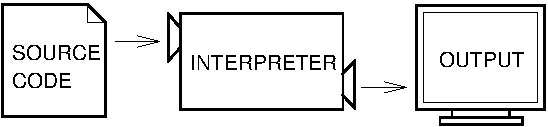
\includegraphics[scale=0.9]{figs/interpret.pdf}}
\caption{An interpreter processes the program a little at a time,
alternately reading lines and performing computations. 
解释器一次只处理程序的一小段,读一行,执行计算,如此交替进行。}
\label{fig.interpret}
\end{figure}

A compiler reads the program and translates it completely before the
program starts running.  In this context, the high-level program is
called the {\bf source code}, and the translated program is called the
{\bf object code} or the {\bf executable}.  Once a program is
compiled, you can execute it repeatedly without further translation.
Figure~\ref{fig.compile} shows the structure of a compiler.

编译器在程序开始运行之前,读取整个程序并且将其全部翻译。
在这种情况下,高级语言程序被称为{\bf 源代码(source code)},
翻译后的程序被称为{\bf 目标代码(object code)}或者{\bf 可执行程序(executable)}。
一旦一个程序被编译,你可以重复的执行它无需再翻译。
图~\ref{fig.compile} 展示了一个编译器的结构。

\begin{figure}
\centerline
{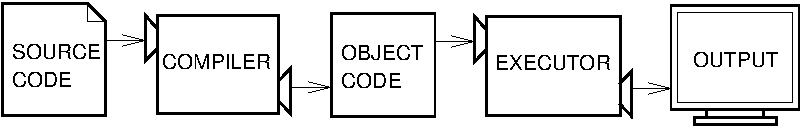
\includegraphics[scale=0.9]{figs/compile.pdf}}
\caption{A compiler translates source code into object code, which is
run by a hardware executor.
编译器将源代码翻译成可被硬件执行的目标代码。}
\label{fig.compile}
\end{figure}

Python is considered an interpreted language because Python programs
are executed by an interpreter.  There are two ways to use the
interpreter: {\bf interactive mode} and {\bf script mode}. In
interactive mode, you type Python programs and the interpreter displays
the result:
\index{interactive mode}
\index{script mode}

Python被认为是解释性语言,因为Python程序由解释器执行。
有两种方法使用解释器:{\bf 交互模式(interactive mode)}和{\bf 脚本模式(script mode)}。
在交互模式下,你键入Python程序,解释器就显示结果:

\begin{verbatim}
>>> 1 + 1
2
\end{verbatim}
%
The chevron, \verb">>>", is the
{\bf prompt} the interpreter uses to indicate that it is ready.  If
you type {\tt 1 + 1}, the interpreter replies {\tt 2}.
\index{prompt}

像军衔样的图标\verb">>>"是{\bf 提示符(prompt)},解释器用其表示它准备好了。
如果你键入{\tt 1 + 1},解释器回复{\tt 2}。

Alternatively, you can store code in a file and use the interpreter to
execute the contents of the file, which is called a {\bf script}.  By
convention, Python scripts have names that end with {\tt .py}.
\index{script}

另外,你也可以将代码存储在一个文件中,其被称为{\bf 脚本(script)},
然后用解释器执行这个文件的内容。习惯上,Python脚本的名字以{\tt .py}结尾。

To execute the script, you have to tell the interpreter the name of
the file.  If you have a script named {\tt dinsdale.py} and you are
working in a UNIX command window, you type {\tt python
dinsdale.py}.  In other development environments, the details of
executing scripts are different.  You can find instructions for
your environment at the Python website \url{http://python.org}.
\index{testing!interactive mode}

为了执行脚本,你必须告诉解释器文件名。
如果你有一个名为{\tt dinsdale.py}的脚本并且你在UNIX命令窗口中工作,
你只要键入{\tt python dinsdale.py}就好了。在其它的开发环境中,
执行脚本的细节不太一样。
你可以在Python网站\url{http://python.org}中找到对于你的环境的说明。

Working in interactive mode is convenient for testing small pieces of
code because you can type and execute them immediately.  But for
anything more than a few lines, you should save your code
as a script so you can modify and execute it in the future.

在交互模式中工作便于测试零散的代码,因为你可以立即键入并且执行它们。
但是对于任何多于几行的代码来说,你应该将你的代码保存为脚本以便将来可以修改再执行。

\section{What is a program? 什么是程序?}

A {\bf program} is a sequence of instructions that specifies how to
perform a computation.  The computation might be something
mathematical, such as solving a system of equations or finding the
roots of a polynomial, but it can also be a symbolic computation, such
as searching and replacing text in a document or (strangely enough)
compiling a program.
\index{program}

一个{\bf 程序(program)}是一串指令,其具体说明如何执行一个计算。
计算可能是一些数学的东西,例如解一个公式系统或者找到一个多项式的根,
而它也可能是一个符号计算,例如在一个文档中搜索并替换文本或者(不可思议地)编译一个程序。

The details look different in different languages, but a few basic
instructions appear in just about every language:

不同语言细节看起来不一样,但是一些基本的指令几乎出现于每个语言当中:

\begin{description}

\item[input:] Get data from the keyboard, a file, or some
other device.

\item[输入:] 从键盘、文件或者其它设备获得数据。

\item[output:] Display data on the screen or send data to a
file or other device.

\item[输出:] 在屏幕上显示数据或者将数据发送到一个文件或其它设备。

\item[math:] Perform basic mathematical operations like addition and
multiplication.

\item[数学:] 执行基本的数学运算,如加法和乘法。

\item[conditional execution:] Check for certain conditions and
execute the appropriate code.

\item[有条件执行:] 检查某一条件并执行相应的代码。

\item[repetition:] Perform some action repeatedly, usually with
some variation.

\item[重复:] 重复执行某些动作,通常有一些变化。

\end{description}

Believe it or not, that's pretty much all there is to it.  Every
program you've ever used, no matter how complicated, is made up of
instructions that look pretty much like these.  So you can think of
programming as the process of breaking a large, complex task
into smaller and smaller subtasks until the subtasks are
simple enough to be performed with one of these basic instructions.
\index{algorithm}

无论你是否相信,这几乎是程序的全部了。
每个你曾经用过的程序,无论多么复杂,都是由跟这些差不多的指令构成的。
因此你可以认为编程就是将大的、复杂的任务分解为越来越小的子任务,
直到这些子任务足够简单,可以被这其中一个基本指令执行。

That may be a little vague, but we will come back to this topic
when we talk about {\bf algorithms}.

这可能有些模糊,但是当我们讨论{\bf 算法(algorithms)}的时候,将回到这些主题。

\section{What is debugging? 什么是调试?}
\index{debugging}
\index{bug}

Programming is error-prone.  For whimsical reasons, programming errors
are called {\bf bugs} and the process of tracking them down is called
{\bf debugging}.
\index{debugging}
\index{bug}

编程是易于出错的。由于比较奇怪的原因,编程的错误被称为{\bf 虫子(bugs)},
并且追踪它们的过程被称为{\bf 捉虫或调试(debugging)}。

Three kinds of errors can occur in a program: syntax errors, runtime 
errors, and semantic errors. It is useful
to distinguish between them in order to track them down more quickly.

程序中有三种错误:语法错误、运行时错误和语义错误。
为了更快的追踪它们,对其进行区分是很有帮助的。

\subsection{Syntax errors 语法错误}
\index{syntax error}
\index{error!syntax}
\index{error message}

Python can only execute a program if the syntax is
correct; otherwise, the interpreter displays an error message.
{\bf Syntax} refers to the structure of a program and the rules about
that structure. \index{syntax} 
For example, parentheses have to come in matching pairs, so
{\tt (1 + 2)} is legal, but {\tt 8)} is a {\bf syntax error}.
\index{parentheses!matching}
\index{syntax}
\index{cummings, e. e.}

Python只能执行语法正确的程序。
否则,解释器显示一个错误信息。
{\bf 语法(Syntax)}指的是一个程序的结构以及关于那些结构的规则。
例如,括号必须成对出现,所以{\tt (1 + 2)}是合法的,
而{\tt 8)}是一个{\bf 语法错误(syntax error)}。

In English readers can tolerate most syntax errors, which is why we
can read the poetry of e. e. cummings without spewing error messages.
Python is not so forgiving.  If there is a single syntax error
anywhere in your program, Python will display an error message and quit,
and you will not be able to run your program. During the first few
weeks of your programming career, you will probably spend a lot of
time tracking down syntax errors.  As you gain experience, you will
make fewer errors and find them faster.

用英语时,读者能容忍大多数语法错误,
这也是为什么我们能读E. E. 卡明斯的诗而不会发出错误信息。
Python就没这么宽容。如果你的程序任何地方有一个语法错误,
Python将显示一个错误信息并且退出,你就不能运行你的程序。
在你编程生涯的前几周,你可能将花很多时间追踪语法错误。
当你更有经验时,你的错误将会变少并且更快的找到它们。

\subsection{Runtime errors 运行时错误}
\label{runtime}

The second type of error is a runtime error, so called because the
error does not appear until after the program has started running.
These errors are also called {\bf exceptions} because they usually
indicate that something exceptional (and bad) has happened.
\index{runtime error}
\index{error!runtime}
\index{exception}
\index{safe language}
\index{language!safe}

第二类错误是运行时错误,之所以这么叫,是因为程序开始运行以后,
这些错误才出现。这些错误也被称为{\bf 异常(exceptions)},
因为它们通常意味着一些异常的(并且是坏的)事情发生了。

Runtime errors are rare in the simple programs you will see in the
first few chapters, so it might be a while before you encounter one.

在前几章简单的程序中很少有运行时错误,因此你可能得有一阵子才会遇到它。

\subsection{Semantic errors 语义错误}
\index{semantics}
\index{semantic error}
\index{error!semantic}
\index{error message}

The third type of error is the {\bf semantic error}.  If there is a
semantic error in your program, it will run successfully in the sense
that the computer will not generate any error messages, but it will
not do the right thing.  It will do something else.  Specifically, it
will do what you told it to do.

第三类错误是{\bf 语义错误(semantic error)}。
如果你的程序中有一个语义错误,在计算机不会生成错误信息的意义上,
它将成功运行。但是,它不会做正确的事情。它将做其它的事情。
特别地,它将做你让它做的事情。

The problem is that the program you wrote is not the program you
wanted to write.  The meaning of the program (its semantics) is wrong.
Identifying semantic errors can be tricky because it requires you to work
backward by looking at the output of the program and trying to figure
out what it is doing.

问题在于你写的程序不是你原本想写的程序。程序的意义(它的语义)是错误的。
识别语义错误可能是棘手的,因为这需要你反过来思考,通过观察程序的输出来搞清楚它在做什么。

\subsection{Experimental debugging 实验性调试}

One of the most important skills you will acquire is debugging.
Although it can be frustrating, debugging is one of the most
intellectually rich, challenging, and interesting parts of
programming.
\index{experimental debugging}
\index{debugging!experimental}

你将获得的最重要的技能之一是调试。
虽然它可能令人泄气,但是调试是编程最富含智慧、挑战以及乐趣的部分之一。

In some ways, debugging is like detective work.  You are confronted
with clues, and you have to infer the processes and events that led
to the results you see.

在某些方面,调试像是侦探工作。
你面对一些线索,你必须推理,是什么过程和事件导致了你看到的结果。

Debugging is also like an experimental science.  Once you have an idea
about what is going wrong, you modify your program and try again.  If
your hypothesis was correct, then you can predict the result of the
modification, and you take a step closer to a working program.  If
your hypothesis was wrong, you have to come up with a new one.  As
Sherlock Holmes pointed out, ``When you have eliminated the
impossible, whatever remains, however improbable, must be the truth.''
(A. Conan Doyle, {\em The Sign of Four})
\index{Holmes, Sherlock}
\index{Doyle, Arthur Conan}

调试也像是一种实验性科学。一旦你有了一个想法,大概哪里出错了,
你就修改你的程序再试一次。
如果你的假设是正确的,那么你就可以预测到修改的结果,并且向好使的程序迈进了一步。
如果你的假设是错误的,你就不得不再提一个新的想法。
如夏洛克·福尔摩斯所指出的:``当你排除了所有的不可能,无论剩下的是什么,
不管多么难以置信,一定是真相。''(阿瑟·柯南·道尔,{\em 《四签名》})
% improbable不应当翻译为不可能,福尔摩斯及其作者是中文读者耳熟能详的人物,应加以翻译

For some people, programming and debugging are the same thing.  That
is, programming is the process of gradually debugging a program until
it does what you want.  The idea is that you should start with a
program that does {\em something} and make small modifications,
debugging them as you go, so that you always have a working program.

对一些人来说,编程和调试是相同的事情。
就是说,编程是逐步调试一个程序的过程,直到它做了你想要的。
这一想法意味着你应该从一个能{\em 做些事情}的程序开始并做小的改动,
随着你进展调试它,这样你总是有一个有效的程序。

For example, Linux is an operating system that contains thousands of
lines of code, but it started out as a simple program Linus Torvalds
used to explore the Intel 80386 chip.  According to Larry Greenfield,
``One of Linus's earlier projects was a program that would switch
between printing AAAA and BBBB.  This later evolved to Linux.''
({\em The Linux Users' Guide} Beta Version 1).
\index{Linux}

例如,Linux是一个操作系统,其包括成千上万行代码,
但是它起始于Linus Torvalds写的一个用于探索Intel 80386芯片的简单程序。
根据Larry Greenfield所说,Linus的早期项目之一是一个交替打印AAAA和BBBB的程序。
这后来演变为了Linux。''({\em Linux用户手册} Beta Version 1)

Later chapters will make more suggestions about debugging and other
programming practices.

后面的章节将给出更多关于调试和其它编程实践的建议。

\section{Formal and natural languages 形式语言和自然语言}
\index{formal language}
\index{natural language}
\index{language!formal}
\index{language!natural}

{\bf Natural languages} are the languages people speak,
such as English, Spanish, and French.  They were not designed
by people (although people try to impose some order on them);
they evolved naturally.

{\bf 自然语言(natural languages)}是人们说的语言,例如英语、西班牙语和法语。
它们不是由人类设计的(虽然人们试图强加一些命令),
它们自然地演变。

{\bf Formal languages} are languages that are designed by people for
specific applications.  For example, the notation that mathematicians
use is a formal language that is particularly good at denoting
relationships among numbers and symbols.  Chemists use a formal
language to represent the chemical structure of molecules.  And
most importantly:

{\bf 形式语言(formal languages)}是由人为了特殊用途设计的。
例如,数学家使用的记号就是形式语言,其特别擅长表示数字和符号之间的关系。
化学家使用他们的形式语言表示分子的化学结构。
最重要的是:

\begin{quote}
{\bf Programming languages are formal languages that have been
designed to express computations.}

{\bf 编程语言是被设计用于表达计算的形式语言。}
\end{quote}

Formal languages tend to have strict rules about syntax.  For example,
$3 + 3 = 6$ is a syntactically correct mathematical statement, but 
$3 + = 3 \mbox{\$} 6$ is not.
$H_2O$ is a syntactically correct
chemical formula, but $_2Zz$ is not.

形式语言倾向于具有严格的语法规则。
例如$3 + 3 = 6$是语法正确的数学表达式,而$3 + = 3 \mbox{\$} 6$则不是。
$H_2O$是语法正确的化学式,而$_2Zz$则不是。

Syntax rules come in two flavors, pertaining to {\bf tokens} and
structure.  Tokens are the basic elements of the language, such as
words, numbers, and chemical elements.  One of the problems with
$3 + = 3 \mbox{\$} 6$ is that \( \$ \) is not a legal token in mathematics
(at least as far as I know).  Similarly, $_2Zz$ is not legal because
there is no element with the abbreviation $Zz$.
\index{token}
\index{structure}

语法规则有关于{\bf 记号(tokens)}和结构的两种类型。
记号是语言的基本元素,例如单词、数字和化学元素。
$3 + = 3 \mbox{\$} 6$的问题之一就是\( \$ \)在数学中不是一个合法的记号
(至少据我所知)。类似的,$_2Zz$也不合法,因为没有一个元素简写为$Zz$。

The second type of syntax error pertains to the structure of a
statement; that is, the way the tokens are arranged.  The statement
$3 + = 3$ is illegal because even though $+$ and $=$ are
legal tokens, you can't have one right after the other.  Similarly,
in a chemical formula the subscript comes after the element name, not
before.

第二种语法错误关于语句的结构。
即记号被安排的方式。语句$3 + = 3$是非法的,因为即使$+$和$=$都是合法的记号,
你也不能把它们俩紧挨在一起。
类似的,在化学式中,下标位于元素之后,而不是在前面。

\begin{exercise}

Write a well-structured English
sentence with invalid tokens in it.  Then write another sentence
with all valid tokens but with invalid structure.

写出一个含有无效记号的英文句子。再写另一个所有记号都有效却包含无效结构的句子。

\end{exercise}

When you read a sentence in English or a statement in a formal
language, you have to figure out what the structure of the sentence is
(although in a natural language you do this subconsciously).  This
process is called {\bf parsing}.
\index{parse}

当你读一个用英语写的句子或者用形式语言写的语句时,
你得了解句子的结构是什么(虽然在自然语言中,你潜意识地做这个)。
这个过程被称作{\bf 分析(parsing)}。

For example, when you hear the sentence, ``The penny dropped,'' you
understand that ``the penny'' is the subject and ``dropped'' is the
predicate.  Once you have parsed a sentence, you can figure out what it
means, or the semantics of the sentence.  Assuming that you know
what a penny is and what it means to drop, you will understand the
general implication of this sentence.

例如,当你听到句子``The penny dropped''时,你理解``the penny''是主语,
``dropped''是谓语。一旦你分析完一个句子,你可以了解它的含义是什么,
或者句子的语义。假如你知道penny是什么以及drop是什么意义,
你将理解这个句子的含义。

Although formal and natural languages have many features in
common---tokens, structure, syntax, and semantics---there are some
differences:
\index{ambiguity}
\index{redundancy}
\index{literalness}

虽然形式语言和自然语言有很多共同的特点---标记、结构、语法以及语义---
它们也有一些不同:

\begin{description}

\item[ambiguity:] Natural languages are full of ambiguity, which
people deal with by using contextual clues and other information.
Formal languages are designed to be nearly or completely unambiguous,
which means that any statement has exactly one meaning,
regardless of context.

\item[歧义性:] 自然语言充满歧义,人们使用上下文线索以及其它信息处理这些歧义。
形式语言被设计成几乎或者完全没有歧义,这意味着不管上下文是什么,
任何语句都只有一个意义。

\item[redundancy:] In order to make up for ambiguity and reduce
misunderstandings, natural languages employ lots of
redundancy.  As a result, they are often verbose.  Formal languages
are less redundant and more concise.

\item[冗余性:] 为了弥补歧义性并且减少误解,自然语言使用很多冗余。
结果,它们经常很冗长。形式语言则冗余较少,更简洁。

\item[literalness:] Natural languages are full of idiom and metaphor.
If I say, ``The penny dropped,'' there is probably no penny and
nothing dropping (this idiom means that someone realized something
after a period of confusion).  Formal languages
mean exactly what they say.

\item[字面性:] 自然语言充满成语和隐喻。如果我说``The penny dropped,'',
可能根本没有便士也没什么东西掉下来(这个成语意思是有人经过一段时间的混乱后,
意识到一些事情)。形式语言含义和它们说的完全一样。

\end{description}

People who grow up speaking a natural language---everyone---often have a
hard time adjusting to formal languages.  In some ways, the difference
between formal and natural language is like the difference between
poetry and prose, but more so:
\index{poetry}
\index{prose}

说自然语言长大的人---所有人---经常一时难于适应形式语言。
在某些方面,形式语言和自然语言之间的不同类似诗歌和散文之间的不同,
但是更重要的是:

\begin{description}

\item[Poetry:] Words are used for their sounds as well as for
their meaning, and the whole poem together creates an effect or
emotional response.  Ambiguity is not only common but often
deliberate.

\item[诗歌:] 单词的含义和声音都有作用,
并且整首诗一起造成一个效果或者情感上的响应。
歧义不但常见,而且经常是故意安排的。

\item[Prose:] The literal meaning of words is more important,
and the structure contributes more meaning.  Prose is more amenable to
analysis than poetry but still often ambiguous.

\item[散文:] 单词表面的含义更重要,结构贡献的比含义更多。
散文比诗歌更适合分析,但仍然经常有歧义。

\item[Programs:] The meaning of a computer program is unambiguous
and literal, and can be understood entirely by analysis of the
tokens and structure.

\item[程序:] 计算机程序的含义是无歧义、无引申义的,
并且能够通过对标记和结构的分析被完全理解。

\end{description}

Here are some suggestions for reading programs (and other formal
languages).  First, remember that formal languages are much more dense
than natural languages, so it takes longer to read them.  Also, the
structure is very important, so it is usually not a good idea to read
from top to bottom, left to right.  Instead, learn to parse the
program in your head, identifying the tokens and interpreting the
structure.  Finally, the details matter.  Small errors in
spelling and punctuation, which you can get away
with in natural languages, can make a big difference in a formal
language.

给你一些阅读程序(以及其它形式语言)的一些建议。
首先,记住形式语言比自然语言稠密的多,因此需要花更长的时间读它们。
其次,结构非常重要,因此从上到下,从左到右的读通常不是一个好的主意。
相反,要学会在你的头脑中分析一个程序,识别记号并且理解结构。
最后,注意细节问题。拼写和标点符号的小错误在自然语言中可以放过,
但是在形式语言中会造成很大的不同。

\section{The first program 第一个程序}
\label{hello}
\index{Hello, World}

Traditionally, the first program you write in a new language
is called ``Hello, World!'' because all it does is display the
words ``Hello, World!''.  In Python, it looks like this:

传统上,你用一门新的语言写的第一个程序叫做``Hello, World!'',
因为它只不过是显示单词``Hello, World!''。
在Python中,它看起来是这个样:

\begin{verbatim}
print 'Hello, World!'
\end{verbatim}
%
This is an example of a {\bf print statement}, which
doesn't actually print anything on paper.  It displays a value on the
screen.  In this case, the result is the words

这是{\bf 打印语句(print statement)}的一个实例,其并不是真的在纸上打印什么东西。
它在屏幕上显示一个值。在此例中,结果是单词:

\begin{verbatim}
Hello, World!
\end{verbatim}
%
The quotation marks in the program mark the beginning and end
of the text to be displayed; they don't appear in the result.
\index{quotation mark}
\index{print statement}
\index{statement!print}

这个程序中的引号标记将要打印的文本之首尾,
它们不会出现在结果中。

In Python 3, the syntax for printing is slightly different:

在Python 3中,打印的语法有些不同:

\begin{verbatim}
print('Hello, World!')
\end{verbatim}
%
The parentheses indicate that {\tt print} is a function.  We'll get
to functions in Chapter~\ref{funcchap}.
\index{function} \index{print function} \index{Python 3}

括号指出{\tt print}是一个函数。
我们将在第~\ref{funcchap}章接触函数。

For the rest of this book, I'll use the print statement.  If you
are using Python 3, you will have to translate.  But other than
that, there are very few differences we have to worry about.

对于本书剩余的部分,我将使用打印语句(而非函数)。
如果你正在使用Python 3,你将必须进行翻译。
但是除此之外,几乎没有什么我们需要担心的不同。

\section{Debugging 调试}
\index{debugging}

It is a good idea to read this book in front of a computer so you can
try out the examples as you go.  You can run most of the examples in
interactive mode, but if you put the code in a script, it is easier
to try out variations.

最好在一台计算机前阅读本书,这样你可以边读书边尝试例子。
你可以在交互模式下运行大多数的例子,但是如果你将代码写入脚本,
就可以更方便的改动它们。

Whenever you are experimenting with a new feature, you should try
to make mistakes.  For example, in the ``Hello, world!'' program,
what happens if you leave out one of the quotation marks?  What
if you leave out both?  What if you spell {\tt print} wrong?
\index{error message}

每当你试验一个新特征的时候,你应该试着犯些错误。
例如,在``Hello, world!''程序中,如果你少写一个引号会发生什么?
如果两个引号都不写呢?如果将{\tt print}拼写错呢?

This kind of experiment helps you remember what you read; it also helps
with debugging, because you get to know what the error messages mean.
It is better to make mistakes now and on purpose than later
and accidentally.

这种实验有助于帮你记住你读到的内容。
它也有助于调试,因为你会知道各种错误信息的含义。
现在故意犯些错误总比将来发生意外的错误好。

Programming, and especially debugging, sometimes brings out strong
emotions.  If you are struggling with a difficult bug, you might 
feel angry, despondent or embarrassed.

编程,特别是调试,有时会带来强烈的情感。
如果你正和一个很难的错误奋战,你可能感到生气、沮丧或尴尬。

There is evidence that people naturally respond to computers as if
they were people.  When they work well, we think
of them as teammates, and when they are obstinate or rude, we
respond to them the same way we respond to rude,
obstinate people (Reeves and Nass, {\it The Media
    Equation: How People Treat Computers, Television, and New Media
    Like Real People and Places}).
\index{debugging!emotional response}
\index{emotional debugging}

有证据表明,人们很自然地对计算机做出响应,仿佛它们就是人。
当它们做得很好的时候,我们认为它们就是队友。
当它们固执或无礼的时候,我们也会像对待固执或无礼的人一样对待它们。
(Reeves and Nass, {\it The Media Equation: 
How People Treat Computers, Television, and New Media 
Like Real People and Places})

Preparing for these reactions might help you deal with them.
One approach is to think of the computer as an employee with
certain strengths, like speed and precision, and
particular weaknesses, like lack of empathy and inability
to grasp the big picture.

对这些反应做好准备有助于你对付它们。
一种方法是将计算机看做是一个雇员,拥有特定的长处,
例如速度和精度,也有些特别的缺点,像缺乏沟通以及不善于把握大局。

Your job is to be a good manager: find ways to take advantage
of the strengths and mitigate the weaknesses.  And find ways
to use your emotions to engage with the problem,
without letting your reactions interfere with your ability
to work effectively.

你的工作是当一个好的管理者:找到充分利用优点,摒弃弱点的方法。
并且找到使用你的情感来解决问题的方法,
不让你的反应干扰你有效工作的能力。

Learning to debug can be frustrating, but it is a valuable skill
that is useful for many activities beyond programming.  At the
end of each chapter there is a debugging section, like this one,
with my thoughts about debugging.  I hope they help!

学习调试可能很令人泄气,
但是它对于许多编程之外的活动也都是一个非常有价值的技能。
在每一章的结尾都会有一节调试内容,比如说这个,
讲述我在调试方面的想法。我希望他们能有用!

\section{Glossary 术语表}

\begin{description}

\item[problem solving(解决问题):]  The process of formulating a problem, finding
a solution, and expressing the solution.
\index{problem solving}

\item[high-level language(高级语言):]  A programming language like Python that
is designed to be easy for humans to read and write.
\index{high-level language}

\item[low-level language(低级语言):]  A programming language that is designed
to be easy for a computer to execute; also called ``machine language'' or
``assembly language.''
\index{low-level language}

\item[portability(可移植性):]  A property of a program that can run on more
than one kind of computer.
\index{portability}

\item[interpret(解释):]  To execute a program in a high-level language
by translating it one line at a time.
\index{interpret}

\item[compile(编译):]  To translate a program written in a high-level language
into a low-level language all at once, in preparation for later
execution.
\index{compile}

\item[source code(源代码):]  A program in a high-level language before
being compiled.
\index{source code}

\item[object code(目标代码):]  The output of the compiler after it translates
the program.
\index{object code}

\item[executable(可执行程序):]  Another name for object code that is ready
to be executed.
\index{executable}

\item[prompt(提示符):] Characters displayed by the interpreter to indicate
that it is ready to take input from the user.
\index{prompt}

\item[script(脚本):] A program stored in a file (usually one that will be
interpreted).
\index{script}

\item[interactive mode(交互模式):] A way of using the Python interpreter by
typing commands and expressions at the prompt.
\index{interactive mode}

\item[script mode(脚本模式):] A way of using the Python interpreter to read
and execute statements in a script.
\index{script mode}

\item[program(程序):] A set of instructions that specifies a computation.
\index{program}

\item[algorithm(算法):]  A general process for solving a category of
problems.
\index{algorithm}

\item[bug(虫子):]  An error in a program.
\index{bug}

\item[debugging(调试):]  The process of finding and removing any of the
three kinds of programming errors.
\index{debugging}

\item[syntax(语法):]  The structure of a program.
\index{syntax}

\item[syntax error(语法错误):]  An error in a program that makes it impossible
to parse (and therefore impossible to interpret).
\index{syntax error}

\item[exception(异常):]  An error that is detected while the program is running.
\index{exception}

\item[semantics(语义):]  The meaning of a program.
\index{semantics}

\item[semantic error(语义错误):]   An error in a program that makes it do something
other than what the programmer intended.
\index{semantic error}

\item[natural language(自然语言):]  Any one of the languages that people speak that
evolved naturally.
\index{natural language}

\item[formal language(形式语言):]  Any one of the languages that people have designed
for specific purposes, such as representing mathematical ideas or
computer programs; all programming languages are formal languages.
\index{formal language}

\item[token(记号):]  One of the basic elements of the syntactic structure of
a program, analogous to a word in a natural language.
\index{token}

\item[parse(分析):]  To examine a program and analyze the syntactic structure.
\index{parse}

\item[print statement(打印语句):]  An instruction that causes the Python
interpreter to display a value on the screen.
\index{print statement}
\index{statement!print}


\end{description}


\section{Exercises 练习题}

\begin{exercise}

Use a web browser to go to the Python website \url{http://python.org}.
This page contains information about Python and links
to Python-related pages, and it gives you the ability to search
the Python documentation.

用网页浏览器打开Python网站\url{http://python.org}.。
这一站点包含了Python的信息和与Python相关页面的链接,而且让你能够搜索Python帮助文档。

For example, if you enter {\tt print} in the search window, the
first link that appears is the documentation of the {\tt print}
statement.  At this point, not all of it will make sense to you,
but it is good to know where it is.

例如,如果你在搜索窗键入{\tt print},出现的第一个链接就是{\tt print}语句的帮助文档。
现在,并不是所有内容都对你有用,不过知道它们在哪里也是很好的。

\index{documentation}
\index{python.org}

\end{exercise}

\begin{exercise}

Start the Python interpreter and type {\tt help()} to start the online
help utility.  Or you can type \verb"help('print')" to get information
about the {\tt print} statement.

打开Python解释器,键入{\tt help()} 可以打开在线帮助工具。
或者你也可以键入\verb"help('print')",来得到关于{\tt print}语句的信息。

If this example doesn't work, you
may need to install additional Python documentation or set an
environment variable; the details depend on your operating system and
version of Python.

如果这一例子不管用,你也许得额外安装Python文档,或者设置环境变量;
具体方式取决于你的操作系统和Python版本。

\index{help utility}

\end{exercise}

\begin{exercise}

Start the Python interpreter and use it as a calculator.
Python's syntax for math operations is almost the same as
standard mathematical notation.  For example, the symbols
{\tt +}, {\tt -} and {\tt /} denote addition, subtraction
and division, as you would expect.  The symbol for
multiplication is {\tt *}.

打开Python解释器,把它当成计算器来使用。
Python关于数学运算的语法跟标准数学符号基本一致。例如,
{\tt +},{\tt -},{\tt /}号表示加,减与除,就像你所期望的那样。乘号是{\tt *}。

If you run a 10 kilometer race in 43 minutes 30 seconds, what is your
average time per mile?  What is your average speed in miles per hour?
(Hint: there are 1.61 kilometers in a mile).

如果你用43分30秒跑了10千米,你每英里所用的平均时间是多少?
你的平均速度用英里每小时表示是多少?(提示:一英里为1.61千米。)

\index{calculator}
\index{running pace}

\end{exercise}




\chapter{Variables, expressions and statements 变量、表达式和语句}

\section{Values and types 值和类型}
\index{value}
\index{type}
\index{string}

A {\bf value} is one of the basic things a program works with,
like a letter or a
number.  The values we have seen so far
are {\tt 1}, {\tt 2}, and
\verb"'Hello, World!'".

{\bf 值(value)}是与程序打交道的基本事物之一,像字母或者数字。
到目前为止,我们已经见过的值有{\tt 1}、{\tt 2}以及\verb"'Hello, World!'"。

These values belong to different {\bf types}:
{\tt 2} is an integer, and \verb"'Hello, World!'" is a {\bf string},
so-called because it contains a ``string'' of letters.
You (and the interpreter) can identify
strings because they are enclosed in quotation marks.
\index{quotation mark}

这些值属于不同的{\bf 类型(types)}:
{\tt 2}是一个整数,\verb"'Hello, World!'"是一个{\bf 字符串(string)},
之所以这么叫,是因为它包括``一串''字母。
你(以及解释器)能识别字符串是因为它们被括在引号中间。

If you are not sure what type a value has, the interpreter can tell you.

如果你不确定一个值具有什么类型,解释器可以告诉你。

\begin{verbatim}
>>> type('Hello, World!')
<type 'str'>
>>> type(17)
<type 'int'>
\end{verbatim}
%
Not surprisingly, strings belong to the type {\tt str} and
integers belong to the type {\tt int}.  Less obviously, numbers
with a decimal point belong to a type called {\tt float},
because these numbers are represented in a
format called {\bf floating-point}.
\index{type}
\index{string type}
\index{type!str}
\index{int type}
\index{type!int}
\index{float type}
\index{type!float}

不奇怪,字符串属于{\tt str}类型,整数属于{\tt int}类型。
不太明显地,具有小数点的数字属于一种被称作{\tt float}的类型,
因为这些数字使用{\bf 浮点(floating-point)}格式表示。

\begin{verbatim}
>>> type(3.2)
<type 'float'>
\end{verbatim}
%
What about values like \verb"'17'" and \verb"'3.2'"?
They look like numbers, but they are in quotation marks like
strings.
\index{quotation mark}

像\verb"'17'"以及\verb"'3.2'"的值是什么类型呢?
它们看起来像数字,但是它们在引号里,像是字符串。

\begin{verbatim}
>>> type('17')
<type 'str'>
>>> type('3.2')
<type 'str'>
\end{verbatim}
%
They're strings.

它们是字符串。

When you type a large integer, you might be tempted to use commas
between groups of three digits, as in {\tt 1,000,000}.  This is not a
legal integer in Python, but it is legal:

当你有一个比较大的整数,你可能想在每三个数字之间使用逗号分隔它,如 {\tt 1,000,000}。
在Python中,这不是一个合法的整数,但是它是合法的:

\begin{verbatim}
>>> 1,000,000
(1, 0, 0)
\end{verbatim}
%
Well, that's not what we expected at all!  Python interprets {\tt
  1,000,000} as a comma-separated sequence of integers.
This is the first example we have seen of a semantic error: the code
runs without producing an error message, but it doesn't do the
``right'' thing.
\index{semantic error}
\index{error!semantic}
\index{error message}

然而,那完全不是我们期望的!
Python将{\tt 1,000,000}解释为逗号分割的一系列整数。
这是我们见到的第一个语义错误的例子:
代码无错误信息地运行,但是它并没有做``正确的''事情。

\section{Variables 变量}
\label{variables}
\index{variable}
\index{assignment statement}
\index{statement!assignment}

One of the most powerful features of a programming language is the
ability to manipulate {\bf variables}.  A variable is a name that
refers to a value.

编程语言最强大的特征之一是操作{\bf 变量(variables)}的能力。
变量是一个名字,它指向某个值。

An {\bf assignment statement} creates new variables and gives
them values:

一个{\bf 赋值语句(assignment statement)}生成新的变量并且将值赋给它们。

\begin{verbatim}
>>> message = 'And now for something completely different'
>>> n = 17
>>> pi = 3.1415926535897932
\end{verbatim}
%
This example makes three assignments.  The first assigns a string
to a new variable named {\tt message};
the second gives the integer {\tt 17} to {\tt n}; the third
assigns the (approximate) value of $\pi$ to {\tt pi}.
\index{state diagram}
\index{diagram!state}

这个例子进行了三次赋值。
第一次将一个字符串赋给一个新的变量名{\tt message};
第二次将整数{\tt 17}赋给{\tt n};
第三次将$\pi$的(近似)值赋给{\tt pi}。

A common way to represent variables on paper is to write the name with
an arrow pointing to the variable's value.  This kind of figure is
called a {\bf state diagram} because it shows what state each of the
variables is in (think of it as the variable's state of mind).
Figure~\ref{fig.state2} shows the result of the previous example.

在纸上表示变量的方法通常是写一个变量名跟着一个箭头指向变量的值。
这种图被称为{\bf 状态图(state diagram)},因为它展示了每个变量所处的状态(将其想为变量的心理状态)。
图~\ref{fig.state2}展示了前面例子的的结果。

\begin{figure}
\centerline
{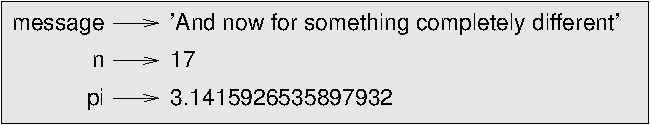
\includegraphics[scale=0.8]{figs/state2.pdf}}
\caption{State diagram.}
\label{fig.state2}
\end{figure}

The type of a variable is the type of the value it refers to.

变量的类型是其所指向值的类型。

\begin{verbatim}
>>> type(message)
<type 'str'>
>>> type(n)
<type 'int'>
>>> type(pi)
<type 'float'>
\end{verbatim}

\begin{exercise}

If you type an integer with a leading zero, you might get
a confusing error:

如果你键入一个以零开头的整数,你可能会得到令你疑惑的错误:

\begin{verbatim}
>>> zipcode = 02492
                  ^
SyntaxError: invalid token
\end{verbatim}

Other numbers seem to work, but the results are bizarre:

别的数字好像能行得通,但是其结果却更奇怪:

\begin{verbatim}
>>> zipcode = 02132
>>> zipcode
1114
\end{verbatim}

Can you figure out what is going on?  Hint: display the
values {\tt 01}, {\tt 010}, {\tt 0100} and {\tt 01000}.

你能说出发生了什么吗?提示:显示这些值 {\tt 01},{\tt 010},{\tt 0100}以及{\tt 01000}。
\index{octal}

\end{exercise}



\section{Variable names and keywords 变量名和关键字}
\index{keyword}

Programmers generally choose names for their variables that
are meaningful---they document what the variable is used for.

程序员通常为变量选择有意义的名字---它们说明了该变量的用途。

Variable names can be arbitrarily long.  They can contain
both letters and numbers, but they have to begin with a letter.
It is legal to use uppercase letters, but it is a good idea
to begin variable names with a lowercase letter (you'll
see why later).

变量名可以任意长。它们可以包括字母和数字,但是必须以字母开始。
使用大写字母是合法的,但是一个变量名以一个小写字母开始是个不错的主意
(后面你会看到原因)。

The underscore character, \verb"_", can appear in a name.
It is often used in names with multiple words, such as
\verb"my_name" or \verb"airspeed_of_unladen_swallow".
\index{underscore character}

下划线字符\verb"_"可以出现在变量名中。
它经常用于有多个单词的变量名,例如\verb"my_name"或者\verb"airspeed_of_unladen_swallow"。

If you give a variable an illegal name, you get a syntax error:

如果你给了变量一个非法的名,将获得一个语法错误:

\begin{verbatim}
>>> 76trombones = 'big parade'
SyntaxError: invalid syntax
>>> more@ = 1000000
SyntaxError: invalid syntax
>>> class = 'Advanced Theoretical Zymurgy'
SyntaxError: invalid syntax
\end{verbatim}
%
{\tt 76trombones} is illegal because it does not begin with a letter.
{\tt more@} is illegal because it contains an illegal character, {\tt
@}.  But what's wrong with {\tt class}?

{\tt 76trombones}是非法的,因为它不是以字母开始的。
{\tt more@}是非法的,因为它包含了一个非法字符{\tt @}。
但是,{\tt class}错在哪儿了呢?

It turns out that {\tt class} is one of Python's {\bf keywords}.  The
interpreter uses keywords to recognize the structure of the program,
and they cannot be used as variable names.
\index{keyword}

实际上,{\tt class}是Python的{\bf 关键字(keywords)}之一。
解释器使用关键字识别程序的结构,它们不能被用作变量名。

Python 2 has 31 keywords:

Python 2有31个关键字:

\begin{verbatim}
and       del       from      not       while    
as        elif      global    or        with     
assert    else      if        pass      yield    
break     except    import    print              
class     exec      in        raise              
continue  finally   is        return             
def       for       lambda    try
\end{verbatim}
%
In Python 3, {\tt exec} is no longer a keyword, but {\tt nonlocal} is.

在Python 3中,{\tt exec}不再是一个关键字,但{\tt nonlocal}是。

You might want to keep this list handy.  If the interpreter complains
about one of your variable names and you don't know why, see if it
is on this list.

你可能想随手携带这个表。如果解释器抱怨你的一个变量名而你不知道为什么,
看一下它是否在这个列表中。

\section{Operators and operands 运算符和运算数}
\index{operator, arithmetic}
\index{arithmetic operator}
\index{operand}
\index{expression}

{\bf Operators} are special symbols that represent computations like
addition and multiplication.  The values the operator is applied to
are called {\bf operands}.

{\bf 运算符(operators)}是特殊的符号,表示类似加法和乘法的计算。
运算符被应用的值被称作{\bf 运算数(operands)}。

The operators {\tt +}, {\tt -}, {\tt *}, {\tt /} and {\tt **}
perform addition, subtraction, multiplication, division and
exponentiation, as in the following examples:

运算符{\tt +}、{\tt -}、{\tt *}、{\tt /}和{\tt **}分别执行加、减、乘、除和指数运算,
如下面的例子:

\begin{verbatim}
20+32   hour-1   hour*60+minute   minute/60   5**2   (5+9)*(15-7)
\end{verbatim}
%
In some other languages, \verb"^" is used for exponentiation, but
in Python it is a bitwise operator called XOR.  I won't cover
bitwise operators in this book, but you can read about
them at \url{http://wiki.python.org/moin/BitwiseOperators}.
\index{bitwise operator}
\index{operator!bitwise}

在一些其它语言中,\verb"^"表示指数运算,
但是在Python中,它表示XOR(异或)位运算。
本书不包括位运算符,
但是你可以在\url{http://wiki.python.org/moin/BitwiseOperators}上阅读关于它们的内容。

In Python 2, the division operator might not do what you expect:

在Python 2中,除法运算符的行为可能不如你所愿:

\begin{verbatim}
>>> minute = 59
>>> minute/60
0
\end{verbatim}
%
The value of {\tt minute} is 59, and in conventional arithmetic 59
divided by 60 is 0.98333, not 0.  The reason for the discrepancy is
that Python is performing {\bf floor division}.
When both of the operands are integers, the result is also an
integer; floor division chops off the fraction
part, so in this example it rounds down to zero.

{\tt minute}的值是59,通常的算数中,59除以60是0.98333而不是0。
造成这一差异的原因是Python执行{\bf 向下取整除(floor division)}。
当两个运算数都是整数时,结果也是整数;
向下取整除会砍掉小数部分,因此此例中其向下舍入成为了0。

In Python 3, the result of this division is a {\tt float}.  The new operator
{\tt //} performs floor division.
\index{Python 3}
\index{floor division}
\index{floating-point division}
\index{division!floor}
\index{division!floating-point}

在Python 3中,这一除法的结果是一个{\tt float}。
新的运算符{\tt //}执行向下取整除。

If either of the operands is a floating-point number, Python performs
floating-point division, and the result is a {\tt float}:

如果其中有一个运算数是浮点数,则Python执行浮点除,结果是{\tt float}:

\begin{verbatim}
>>> minute/60.0
0.98333333333333328
\end{verbatim}


\section{Expressions and statements 表达式和语句}

An {\bf expression} is a combination of values, variables, and operators.
A value all by itself is considered an expression, and so is
a variable, so the following are all legal expressions
(assuming that the variable {\tt x} has been assigned a value):
\index{expression}
\index{evaluate}

一个{\bf 表达式(expression)}是值、变量和运算符的组合。
值自身被认为是一个表达式,变量也是,因此下面都是合法的表达式
(假设变量{\tt x}已经被赋值了):

\begin{verbatim}
17
x
x + 17
\end{verbatim}
%
A {\bf statement} is a unit of code that the Python interpreter can
execute.  We have seen two kinds of statement: print and
assignment.

一条{\bf 语句(statement)}是一个Python解释器可以执行的代码单元。
你已经见过两种语句了:打印和赋值。

Technically an expression is also a statement, but it is probably
simpler to think of them as different things.  The important difference
is that an expression has a value; a statement does not.

技术上讲,一个表达式也是一条语句,但是将他们看作不同的东西可能会更简单。
重要的不同是表达式具有一个值;语句没有。

\section{Interactive mode and script mode 交互模式和脚本模式}

One of the benefits of working with an interpreted language is that
you can test bits of code in interactive mode before you put them
in a script.  But there are differences between interactive mode
and script mode that can be confusing.
\index{interactive mode}
\index{script mode}

使用解释型语言的一个好处是,在你将一段代码放入脚本之前,
你可以在交互模式下测试一下。
但是交互模式和脚本模式之间也有不同,容易搞混。

For example, if you are using Python as a calculator, you might type

例如,如果你正将Python用作计算器,你可能键入:

\begin{verbatim}
>>> miles = 26.2
>>> miles * 1.61
42.182
\end{verbatim}

The first line assigns a value to {\tt miles}, but it has no visible
effect.  The second line is an expression, so the interpreter
evaluates it and displays the result.  So we learn that a marathon is
about 42 kilometers.

第一行将一个值赋给{\tt miles},但是并没有显示效果。
第二行是一个表达式,因此解释器计算它并将结果显示出来。
所以我们学到,一段马拉松大概是42公里。

But if you type the same code into a script and run it, you get no
output at all.  In script mode an expression, all by itself, has no
visible effect.  Python actually evaluates the expression, but it doesn't
display the value unless you tell it to:

但是如果你将相同的代码键入一个脚本并且运行它,你将根本不能获得输出。
在完全的脚本模式下,表达式不会有显示效果。
Python实际上计算了表达式,但是如果你不告诉它,它不会显示结果。

\begin{verbatim}
miles = 26.2
print miles * 1.61
\end{verbatim}

This behavior can be confusing at first.

此行为开始可能有些令人茫然。

A script usually contains a sequence of statements.  If there
is more than one statement, the results appear one at a time
as the statements execute.

一个脚本通常包括一系列语句。
如果有多于一条的语句,那么每条语句执行后都显示结果。

For example, the script

例如脚本

\begin{verbatim}
print 1
x = 2
print x
\end{verbatim}
%
produces the output

产生输出

\begin{verbatim}
1
2
\end{verbatim}
%
The assignment statement produces no output.

赋值语句不产生输出。

\begin{exercise}

Type the following statements in the Python interpreter to see
what they do:

在Python解释器中键入以下的语句,看看他们的功能:

\begin{verbatim}
5
x = 5
x + 1
\end{verbatim}
%
Now put the same statements into a script and run it.  What
is the output?  Modify the script by transforming each
expression into a print statement and then run it again.

现在将同样的语句写入一个脚本中并执行它。输出是什么?
修改脚本,将每个表达式变成打印语句,再次运行它。
\end{exercise}


\section{Order of operations 运算的顺序}
\index{order of operations}
\index{rules of precedence}
\index{PEMDAS}

When more than one operator appears in an expression, the order of
evaluation depends on the {\bf rules of precedence}.  For
mathematical operators, Python follows mathematical convention.
The acronym {\bf PEMDAS} is a useful way to
remember the rules:
\index{parentheses!overriding precedence}

当一个表达式中有多于一个运算符时,计算的顺序依赖{\bf 优先级规则(rules of precedence)}。
对于算数运算,Python遵循数学的惯例。
缩写 {\bf PEMDAS}有助于记住这一规则:

\begin{itemize}

\item {\bf P}arentheses have the highest precedence and can be used 
to force an expression to evaluate in the order you want. Since
expressions in parentheses are evaluated first, {\tt 2 * (3-1)} is 4,
and {\tt (1+1)**(5-2)} is 8. You can also use parentheses to make an
expression easier to read, as in {\tt (minute * 100) / 60}, even
if it doesn't change the result.

\item 括号({\bf P}arentheses)具有最高的优先级,并且可以被用于强制表达式按你需要的顺序计算。
既然在括号中的表达式首先被计算,那么{\tt 2 * (3-1)}是4,{\tt (1+1)**(5-2)}是8。
你也可以用括号使得一个表达式更易读,如{\tt (minute * 100) / 60},即使它并不改变运算的结果。

\item {\bf E}xponentiation has the next highest precedence, so
{\tt 2**1+1} is 3, not 4, and {\tt 3*1**3} is 3, not 27.

\item 指数运算({\bf E}xponentiation)具有次高的优先级,因此{\tt 2**1+1}是3而非4,
{\tt 3*1**3}是3而非27。

\item {\bf M}ultiplication and {\bf D}ivision have the same precedence,
which is higher than {\bf A}ddition and {\bf S}ubtraction, which also
have the same precedence.  So {\tt 2*3-1} is 5, not 4, and
{\tt 6+4/2} is 8, not 5.

\item 乘法({\bf M}ultiplication)和除法({\bf D}ivision)有相同的优先级,
比加法({\bf A}ddition)和减法({\bf S}ubtraction)高,加法和减法也具有相同的优先级。
因此{\tt 2*3-1}是5而非4,{\tt 6+4/2}是8而非5。

\item Operators with the same precedence are evaluated from left to
  right (except exponentiation).  So in the expression {\tt degrees /
    2 * pi}, the division happens first and the result is multiplied
  by {\tt pi}.  To divide by $2 \pi$, you can use parentheses or write
  {\tt degrees / 2 / pi}.
  
\item 具有相同优先级的运算符按照从左到右的顺序进行计算(除了指数运算)。
因此表达式{\tt degrees / 2 * pi}中,除法先运算,然后结果被乘以{\tt pi}。
为了被$2 \pi$除,你可以使用括号,或者写成{\tt degrees / 2 / pi}。

\end{itemize}

I don't work very hard to remember rules of precedence for other
operators.  If I can't tell by looking at the expression, I use
parentheses to make it obvious.

我并没有费力去记住其它运算符的优先级规则。
如果通过观察表达式,我不能说清楚,我使用括号使其变得更明显。

\section{String operations 字符串运算}
\index{string!operation}
\index{operator!string}

In general, you can't perform mathematical operations on strings, even
if the strings look like numbers, so the following are illegal:

一般来讲,你不能对字符串执行数学运算,即使字符串看起来很像数字,
因此下面是非法的:

\begin{verbatim}
'2'-'1'    'eggs'/'easy'    'third'*'a charm'
\end{verbatim}
%
The {\tt +} operator works with strings, but it
might not do what you expect: it performs
{\bf concatenation}, which means joining the strings by
linking them end-to-end.  For example:
\index{concatenation}

{\tt +}运算符可用于字符串,但是它可能不会做你所期望的事情:
它执行{\bf 级联(concatenation)}运算,也就是将字符串端到端的连起来。
例如:

\begin{verbatim}
first = 'throat'
second = 'warbler'
print first + second
\end{verbatim}
%
The output of this program is {\tt throatwarbler}.

程序的输出是{\tt throatwarbler}。

The {\tt *} operator also works on strings; it performs repetition.
For example, \verb"'Spam'*3" is \verb"'SpamSpamSpam'".  If one of the operands
is a string, the other has to be an integer.

{\tt *}运算符也可应用于字符串;它执行重复运算。
例如,\verb"'Spam'*3"的结果是\verb"'SpamSpamSpam'"。
如果其中一个运算数是字符串,则另外一个必须是整数。

This use of {\tt +} and {\tt *} makes sense by
analogy with addition and multiplication.  Just as {\tt 4*3} is
equivalent to {\tt 4+4+4}, we expect \verb"'Spam'*3" to be the same as
\verb"'Spam'+'Spam'+'Spam'", and it is.  On the other hand, there is a
significant way in which string concatenation and repetition are
different from integer addition and multiplication.
Can you think of a property that addition has
that string concatenation does not?
\index{commutativity}

{\tt +}和{\tt *}的使用类比加法和乘法也讲得通。
就像由于{\tt 4*3}与{\tt 4+4+4}等价,
我们就希望\verb"'Spam'*3"和\verb"'Spam'+'Spam'+'Spam'"一样,而它确实是这样。
另一方面,字符串的级联和重复与整数的加法和乘法截然不同。
你能想出来一个加法具有,而级联不具有的性质么?

\section{Comments 注释}
\index{comment}

As programs get bigger and more complicated, they get more difficult
to read.  Formal languages are dense, and it is often difficult to
look at a piece of code and figure out what it is doing, or why.

随着程序变得越来越大,越来越复杂,它们变得越来越难读。
形式语言是稠密的,读一段代码并说出其做什么或者为什么这样通常很难。

For this reason, it is a good idea to add notes to your programs to explain
in natural language what the program is doing.  These notes are called
{\bf comments}, and they start with the \verb"#" symbol:

因此,在你的程序中用自然语言做笔记,来解释程序做什么通常是比较好的办法。
这些标注被称为{\bf 注释(comments)},其以\verb"#"符号开始。

\begin{verbatim}
# compute the percentage of the hour that has elapsed
percentage = (minute * 100) / 60
\end{verbatim}
%
In this case, the comment appears on a line by itself.  You can also put
comments at the end of a line:

此例中,注释独立一行。你也可以将注释放在行尾:

\begin{verbatim}
percentage = (minute * 100) / 60     # percentage of an hour
\end{verbatim}
%
Everything from the {\tt \#} to the end of the line is ignored---it
has no effect on the program.

从{\tt \#}开始到行尾的所有东西都被忽略了---其对程序没有影响。

Comments are most useful when they document non-obvious features of
the code.  It is reasonable to assume that the reader can figure out
{\em what} the code does; it is much more useful to explain {\em why}.

当注释写出代码不明显的特征的时候最有效。
假设读者能够指出代码做了{\em 什么}通常比较适当;
解释{\em 为什么}则更有用。

This comment is redundant with the code and useless:

下面这个注释是代码的重复而且没有什么用:

\begin{verbatim}
v = 5     # assign 5 to v
\end{verbatim}
%
This comment contains useful information that is not in the code:

下面的注释包括包含了代码中没有的有用信息:

\begin{verbatim}
v = 5     # velocity in meters/second. 
\end{verbatim}
%
Good variable names can reduce the need for comments, but
long names can make complex expressions hard to read, so there is
a tradeoff.

好的变量名能够减少对注释的需求,但是长变量名使得表达式很难读,
因此这有个均衡问题。

\section{Debugging 调试}
\index{debugging}

At this point the syntax error you are most likely to make is
an illegal variable name, like {\tt class} and {\tt yield}, which
are keywords, or \verb"odd~job" and \verb"US$", which contain
illegal characters.
\index{syntax error}
\index{error!syntax}

此时你经常犯的语法错误是非法变量名,如{\tt class}和{\tt yield}是关键字,
\verb"odd~job"和\verb"US$"包含了非法字符。

If you put a space in a variable name, Python thinks it is two
operands without an operator:

如果你在变量名中间放了一个空格,Python认为它是两个没有运算符的运算数。

\begin{verbatim}
>>> bad name = 5
SyntaxError: invalid syntax
\end{verbatim}
%
For syntax errors, the error messages don't help much.
The most common messages are {\tt SyntaxError: invalid syntax} and
{\tt SyntaxError: invalid token}, neither of which is very informative.
\index{error message}
\index{use before def}
\index{exception}
\index{runtime error}
\index{error!runtime}

对于语法错误,错误信息帮助不大。
最常见的信息是{\tt SyntaxError: invalid syntax}以及
{\tt SyntaxError: invalid token},这两个都没什么信息量。

The runtime error you are most likely to make is a ``use before
def;'' that is, trying to use a variable before you have assigned
a value.  This can happen if you spell a variable name wrong:

你最容易犯的运行时错误是``定义前使用'',也就是说试图在对一个变量赋值前使用它。
如果你拼写错了变量名这就可能发生。

\begin{verbatim}
>>> principal = 327.68
>>> interest = principle * rate
NameError: name 'principle' is not defined
\end{verbatim}
%
Variables names are case sensitive, so {\tt LaTeX} is not the
same as {\tt latex}.
\index{case-sensitivity, variable names}
\index{semantic error}
\index{error!semantic}

变量名是大小写敏感的,因此{\tt LaTeX}和{\tt latex}不一样。

At this point the most likely cause of a semantic error is
the order of operations.  For example, to evaluate
 $\frac{1}{2 \pi}$,
you might be tempted to write

此时最容易引起的语义错误是运算的顺序。
例如,为了计算$\frac{1}{2 \pi}$,你可能写成

\begin{verbatim}
>>> 1.0 / 2.0 * pi
\end{verbatim}
%
But the division happens first, so you would get $\pi / 2$, which
is not the same thing!  There is no way for Python
to know what you meant to write, so in this case you don't
get an error message; you just get the wrong answer.
\index{order of operations}

但是,首先进行除法运算,因此你得到了$\pi / 2$,这并不是一回事儿!
对于Python,它没有办法知道你的意图是写什么,因此此例中你不会获得错误信息;
你只会获得错误的结果。

\section{Glossary 术语表}

\begin{description}

\item[value(值):]  One of the basic units of data, like a number or string, 
that a program manipulates.
\index{value}

\item[type(类型):] A category of values.  The types we have seen so far
are integers (type {\tt int}), floating-point numbers (type {\tt
float}), and strings (type {\tt str}).
\index{type}

\item[integer(整数):] A type that represents whole numbers.
\index{integer}

\item[floating-point(浮点):] A type that represents numbers with fractional
parts.
\index{floating-point}

\item[string(字符串):] A type that represents sequences of characters.
\index{string}

\item[variable(变量):]  A name that refers to a value.
\index{variable}

\item[statement(语句):]  A section of code that represents a command or action.  So
far, the statements we have seen are assignments and print statements.
\index{statement}

\item[assignment(赋值):]  A statement that assigns a value to a variable.
\index{assignment}

\item[state diagram(状态图):]  A graphical representation of a set of variables and the
values they refer to.
\index{state diagram}

\item[keyword(关键字):]  A reserved word that is used by the compiler to parse a
program; you cannot use keywords like {\tt if}, {\tt  def}, and {\tt while} as
variable names.
\index{keyword}

\item[operator(运算符):]  A special symbol that represents a simple computation like
addition, multiplication, or string concatenation.
\index{operator}

\item[operand(运算数):]  One of the values on which an operator operates.
\index{operand}

\item[floor division(向下取整除):] The operation that divides two numbers and chops off
the fraction part.
\index{floor division}

\item[expression(表达式):]  A combination of variables, operators, and values that
represents a single result value.
\index{expression}

\item[evaluate(计算):]  To simplify an expression by performing the operations
in order to yield a single value.

\item[rules of precedence(优先级规则):]  The set of rules governing the order in which
expressions involving multiple operators and operands are evaluated.
\index{rules of precedence}
\index{precedence}

\item[concatenate(级联):]  To join two operands end-to-end.
\index{concatenation}

\item[comment(注释):]  Information in a program that is meant for other
programmers (or anyone reading the source code) and has no effect on the
execution of the program.
\index{comment}

\end{description}


\section{Exercises}

\begin{exercise}

Assume that we execute the following assignment statements:

假设我们执行如下的赋值语句:

\begin{verbatim}
width = 17
height = 12.0
delimiter = '.'
\end{verbatim}

For each of the following expressions, write the value of the
expression and the type (of the value of the expression).

对下列每一个表达式,写出表达式的值和(表达式的值所具备的)类型。

\begin{enumerate}

\item {\tt width/2}

\item {\tt width/2.0}

\item {\tt height/3}

\item {\tt 1 + 2 * 5}

\item {\tt delimiter * 5}

\end{enumerate}

Use the Python interpreter to check your answers.

使用Python解释器来检查你的答案。
\end{exercise}

\begin{exercise}

Practice using the Python interpreter as a calculator: 

练习将Python解释器当作计算器使用:
\index{calculator}

\begin{enumerate}

\item The volume of a sphere with radius $r$ is $\frac{4}{3} \pi r^3$.
  What is the volume of a sphere with radius 5?  Hint: 392.7 is wrong!

\item 半径为$r$的球体积是$\frac{4}{3} \pi r^3$。
    半径为5的球体积是多少?提示:392.7是错误答案!

\item Suppose the cover price of a book is \$24.95, but bookstores get a
  40\% discount.  Shipping costs \$3 for the first copy and 75 cents
  for each additional copy.  What is the total wholesale cost for
  60 copies?

\item 假设一本书的零售价是\$24.95,但书店有40\%的折扣。运费则是第一本\$3,以后每本75美分。
    购买60本的总价是多少?

\item If I leave my house at 6:52 am and run 1 mile at an easy pace
  (8:15 per mile), then 3 miles at tempo (7:12 per mile) and 1 mile at
  easy pace again, what time do I get home for breakfast?

\item 如果我上午6:52离开家,以随意的节奏跑1英里(每英里8:15),再以
    较快速度跑3英里(每英里7:12),之后又以随意的节奏跑1英里,我什么时候回到家吃早饭?
\index{running pace}

\end{enumerate}
\end{exercise}


%Last Time
\chapter{Functions 函数}
\label{funcchap}

\section{Function calls 函数调用}
\label{functionchap}
\index{function call}

In the context of programming, a {\bf function} is a named sequence of
statements that performs a computation.  When you define a function,
you specify the name and the sequence of statements.  Later, you can
``call'' the function by name.  
We have already seen one example of a {\bf function call}:

在编程的语境下,{\bf 函数(function)}是对一序列执行计算的语句的命名。
当你定义一个函数的时候,你指定了名字和语句序列。
随后,你可以通过名字``调用''该函数。
我们已经见过了一个{\bf 函数调用(function call)}的例子。

\begin{verbatim}
>>> type(32)
<type 'int'>
\end{verbatim}
%
The name of the function is {\tt type}.  The expression in parentheses
is called the {\bf argument} of the function.  The result, for this
function, is the type of the argument.
\index{parentheses!argument in}

函数名是{\tt type}。括号中的表达是被称为函数的{\bf 实参(argument)}。
此函数的结果是实参的类型。

It is common to say that a function ``takes'' an argument and ``returns''
a result.  The result is called the {\bf return value}.
\index{argument}
\index{return value}

人们常说函数``接受''实参并且``返回''一个结果。
该结果被称为{\bf 返回值(return value)}


\section{Type conversion functions 类型转换函数}
\index{conversion!type}
\index{type conversion}

% from Elkner:
% comment on whether these things are _really_ functions?
% use max as an example of a built-in?

% my reply:
% they are on the list of ``built-in functions'' so I am
% willing to call them functions.

Python provides built-in functions that convert values
from one type to another.  The {\tt int} function takes any value and
converts it to an integer, if it can, or complains otherwise:
\index{int function}
\index{function!int}

Python提供内建函数将值从一种类型转换为另一种类型。
函数{\tt int}接受任意值,并在其能做到的情况下,将该任意值转换成一个整数,
否则会抗议:

\begin{verbatim}
>>> int('32')
32
>>> int('Hello')
ValueError: invalid literal for int(): Hello
\end{verbatim}
%
{\tt int} can convert floating-point values to integers, but it
doesn't round off; it chops off the fraction part:

{\tt int}能将浮点数转换为整数,但是它并不完美,截掉了小数部分:

\begin{verbatim}
>>> int(3.99999)
3
>>> int(-2.3)
-2
\end{verbatim}
%
{\tt float} converts integers and strings to floating-point
numbers:
\index{float function}
\index{function!float}

{\tt float}将整数或者字符串转化为浮点数:

\begin{verbatim}
>>> float(32)
32.0
>>> float('3.14159')
3.14159
\end{verbatim}
%
Finally, {\tt str} converts its argument to a string:
\index{str function}
\index{function!str}

最后,{\tt str}将实参转成字符串。

\begin{verbatim}
>>> str(32)
'32'
>>> str(3.14159)
'3.14159'
\end{verbatim}
%



\section{Math functions 数学函数}
\index{math function}
\index{function, math}

Python has a math module that provides most of the familiar
mathematical functions.  A {\bf module} is a file that contains a
collection of related functions.
\index{module}
\index{module object}

Python有数学模块,其提供了大部分熟悉的数学函数。
{\bf 模块(module)}是一个包含一批相关函数的文件。

Before we can use the module, we have to import it:

在我们使用模块之前,需要导入它:

\begin{verbatim}
>>> import math
\end{verbatim}
%
This statement creates a {\bf module object} named math.  If
you print the module object, you get some information about it:

这条语句生成一个名为math的{\bf 模块对象(module object)}。
如果你打印这个模块对象,你将获得关于它的一些信息:

\begin{verbatim}
>>> print math
<module 'math' (built-in)>
\end{verbatim}
%
The module object contains the functions and variables defined in the
module.  To access one of the functions, you have to specify the name
of the module and the name of the function, separated by a dot (also
known as a period).  This format is called {\bf dot notation}.
\index{dot notation}

该模块对象包括定义在模块内的函数和变量。
为了访问其中一个函数,你必须指出该模块的名字以及函数名,
并以点(也被称作句号)分割。
这种格式被称作{\bf 点记法(dot notation)}。

\begin{verbatim}
>>> ratio = signal_power / noise_power
>>> decibels = 10 * math.log10(ratio)

>>> radians = 0.7
>>> height = math.sin(radians)
\end{verbatim}
%
The first example uses \verb"log10" to compute 
a signal-to-noise ratio in decibels (assuming that \verb"signal_power" and
\verb"noise_power" are defined).  The math module also provides {\tt log},
which computes logarithms base {\tt e}.
\index{log function}
\index{function!log}
\index{sine function}
\index{radian}
\index{trigonometric function}
\index{function, trigonometric}

第一个例子使用\verb"log10"计算分贝信噪比(假设\verb"signal_power"和\verb"noise_power"已经被定义了)。
math模块也提供了{\tt log}函数,其计算以{\tt e}为底的对数。

The second example finds the sine of {\tt radians}.  The name of the
variable is a hint that {\tt sin} and the other trigonometric
functions ({\tt cos}, {\tt tan}, etc.)  take arguments in radians. To
convert from degrees to radians, divide by 360 and multiply by
$2 \pi$:

第二个例子计算{\tt radians}的sine值。
变量名暗示{\tt sin}函数以及其它三角函数({\tt cos}、{\tt tan}等)接受弧度参数。
为了从度转为弧度,除以360并乘以$2 \pi$:

\begin{verbatim}
>>> degrees = 45
>>> radians = degrees / 360.0 * 2 * math.pi
>>> math.sin(radians)
0.707106781187
\end{verbatim}
%
The expression {\tt math.pi} gets the variable {\tt pi} from the math
module.  The value of this variable is an approximation
of $\pi$, accurate to about 15 digits.
\index{pi}

表达式{\tt math.pi}从math模块中获得变量{\tt pi}。
该变量的值是对$\pi$的近似,精度大约15位数。

If you know
your trigonometry, you can check the previous result by comparing it to
the square root of two divided by two:
\index{sqrt function}
\index{function!sqrt}

如果你懂几何学,你可以通过将之前的结果和2的平方根再除以2进行比较:

\begin{verbatim}
>>> math.sqrt(2) / 2.0
0.707106781187
\end{verbatim}
%

\section{Composition 组合}
\index{composition}

So far, we have looked at the elements of a program---variables,
expressions, and statements---in isolation, without talking about how to
combine them.

目前为止,我们已经分别看到了程序的基本元素---变量、表达式和语句---
还没有讨论如何组合它们。

One of the most useful features of programming languages is their
ability to take small building blocks and {\bf compose} them.  For
example, the argument of a function can be any kind of expression,
including arithmetic operators:

程序设计语言的最有用特征之一是分解成小块并将其{\bf 组合(compose)}的能力。
例如,函数的实参能够接受任何类型的表达式,包括算数运算符:

\begin{verbatim}
x = math.sin(degrees / 360.0 * 2 * math.pi)
\end{verbatim}
%
And even function calls:

甚至函数调用:

\begin{verbatim}
x = math.exp(math.log(x+1))
\end{verbatim}
%
Almost anywhere you can put a value, you can put an arbitrary
expression, with one exception: the left side of an assignment
statement has to be a variable name.  Any other expression on the left
side is a syntax error (we will see exceptions to this rule
later).

你几乎可以将一个任意值、表达式,放在任何地方,除了一个例外:
赋值语句的左侧必须是一个变量名,任何其它的表达式都是语法错误的
(后面我们会看到这个例外的规则)。

\begin{verbatim}
>>> minutes = hours * 60                 # right
>>> hours * 60 = minutes                 # wrong!
SyntaxError: can't assign to operator
\end{verbatim}
%
\index{SyntaxError}
\index{exception!SyntaxError}


\section{Adding new functions 增加新函数}

So far, we have only been using the functions that come with Python,
but it is also possible to add new functions.
A {\bf function definition} specifies the name of a new function and
the sequence of statements that execute when the function is called.
\index{function}
\index{function definition}
\index{definition!function}

目前为止,我们只了使用Python自带的函数,
但是增加新函数也是可能的。
一个{\bf 函数定义(function definition)}指出新函数的名
以及当函数被调用时执行的语句序列。

Here is an example:

这是一个例子:

\begin{verbatim}
def print_lyrics():
    print "I'm a lumberjack, and I'm okay."
    print "I sleep all night and I work all day."
\end{verbatim}
%
{\tt def} is a keyword that indicates that this is a function
definition.  The name of the function is \verb"print_lyrics".  The
rules for function names are the same as for variable names: letters,
numbers and some punctuation marks are legal, but the first character
can't be a number.  You can't use a keyword as the name of a function,
and you should avoid having a variable and a function with the same
name.
\index{def keyword}
\index{keyword!def}
\index{argument}

{\tt def}是一个关键字,其指明这是一个函数定义。
函数名是\verb"print_lyrics"。
函数的命名规则和变量名相同:字母、数字以及一些标点符号是合法的,
但是第一个字符不能是数字。不能使用关键字作为函数名,并应该避免
一个变量和一个函数同名。

The empty parentheses after the name indicate that this function
doesn't take any arguments.
\index{parentheses!empty}
\index{header}
\index{body}
\index{indentation}
\index{colon}

函数名后面的空括号表明该函数不接受任何实参。

The first line of the function definition is called the {\bf header};
the rest is called the {\bf body}.  The header has to end with a colon
and the body has to be indented.  By convention, the indentation is
always four spaces (see Section~\ref{editor}).  The body can contain
any number of statements.

函数定义的第一行被称作{\bf 函数头(header)};
其余部分被称作{\bf 函数体(body)}。
函数体必须以冒号结尾,函数体必须是缩进的。
按照惯例,缩进经常是4个空格(见\ref{editor}节)。
函数体能包含任意条语句。

The strings in the print statements are enclosed in double
quotes.  Single quotes and double quotes do the same thing;
most people use single quotes except in cases like this where
a single quote (which is also an apostrophe) appears in the string.
\index{ellipses}

打印语句中的字符串被括在双引号中。单引号和双引号做同样的事情。
大多数人使用单引号,除了类似这里的情况,即单引号(也表示撇号)出现在字符串中。

If you type a function definition in interactive mode, the interpreter
prints ellipses ({\em ...}) to let you know that the definition
isn't complete:

如果你在交互模式中键入函数定义,解释器打印省略号({\em ...}),
以便让你知道定义并不完整。

\begin{verbatim}
>>> def print_lyrics():
...     print "I'm a lumberjack, and I'm okay."
...     print "I sleep all night and I work all day."
...
\end{verbatim}
%
To end the function, you have to enter an empty line (this is
not necessary in a script).

为了结束函数,你必须输入一个空行(这在脚本中不是必须的)。

Defining a function creates a variable with the same name.

定义一个函数生成一个同名的变量。

\begin{verbatim}
>>> print print_lyrics
<function print_lyrics at 0xb7e99e9c>
>>> type(print_lyrics)
<type 'function'>
\end{verbatim}
%
The value of \verb"print_lyrics" is a {\bf function object}, which
has type \verb"'function'".
\index{function object}
\index{object!function}

\verb"print_lyrics"的值是一个{\bf 函数对象(function object)},
其类型是\verb"'function'"。

The syntax for calling the new function is the same as
for built-in functions:

调用新函数的语法和调用内建函数的相同:

\begin{verbatim}
>>> print_lyrics()
I'm a lumberjack, and I'm okay.
I sleep all night and I work all day.
\end{verbatim}
%
Once you have defined a function, you can use it inside another
function.  For example, to repeat the previous refrain, we could write
a function called \verb"repeat_lyrics":

一旦你定义了一个函数,你可以在另一个函数内部使用它。
例如,为了重复之前的叠句,我们可以写一个叫\verb"repeat_lyrics"的函数:

\begin{verbatim}
def repeat_lyrics():
    print_lyrics()
    print_lyrics()
\end{verbatim}
%
And then call \verb"repeat_lyrics":

然后调用\verb"repeat_lyrics":

\begin{verbatim}
>>> repeat_lyrics()
I'm a lumberjack, and I'm okay.
I sleep all night and I work all day.
I'm a lumberjack, and I'm okay.
I sleep all night and I work all day.
\end{verbatim}
%
But that's not really how the song goes.

但那不是这首歌本来的样子。

\section{Definitions and uses 定义和使用}
\index{function definition}

Pulling together the code fragments from the previous section, the
whole program looks like this:

汇集上一节的代码切片,整个程序看起来像这样:

\begin{verbatim}
def print_lyrics():
    print "I'm a lumberjack, and I'm okay."
    print "I sleep all night and I work all day."

def repeat_lyrics():
    print_lyrics()
    print_lyrics()

repeat_lyrics()
\end{verbatim}
%
This program contains two function definitions: \verb"print_lyrics" and
\verb"repeat_lyrics".  Function definitions get executed just like other
statements, but the effect is to create function objects.  The statements
inside the function do not get executed until the function is called, and
the function definition generates no output.
\index{use before def}

该程序包含两个函数定义:\verb"print_lyrics"和\verb"repeat_lyrics"。
函数定义就像其它语句执行一样,但是左右是生成函数对象。
函数内部的语句直到被调用才会被执行,并且函数定义没有任何输出。

As you might expect, you have to create a function before you can
execute it.  In other words, the function definition has to be
executed before the first time it is called.

和你所期望的一样,函数执行之前,你必须生成它。
换句话说,函数定义必须在其第一次调用之前执行。

\begin{exercise}

Move the last line of this program
to the top, so the function call appears before the definitions. Run 
the program and see what error
message you get.

\end{exercise}

\begin{exercise}

Move the function call back to the bottom
and move the definition of \verb"print_lyrics" after the definition of
\verb"repeat_lyrics".  What happens when you run this program?

\end{exercise}


\section{Flow of execution 执行流程}
\index{flow of execution}

In order to ensure that a function is defined before its first use,
you have to know the order in which statements are executed, which is
called the {\bf flow of execution}.

为了保证函数第一次使用之前被定义,你必须要知道语句被执行的顺序,
这也被称作{\bf 执行流程(flow of execution)}。

Execution always begins at the first statement of the program.
Statements are executed one at a time, in order from top to bottom.

执行总是开始于程序的第一条语句。自顶向下,每次执行一条语句。

Function definitions do not alter the flow of execution of the
program, but remember that statements inside the function are not
executed until the function is called.

函数定义不改变程序执行的流程,但是请记住函数内部的语句直到该函数被调用时才执行。

A function call is like a detour in the flow of execution. Instead of
going to the next statement, the flow jumps to the body of
the function, executes all the statements there, and then comes back
to pick up where it left off.

函数调用像是在执行流程上饶了一个弯路。
流程不是到下一条语句,而是跳入函数体,执行那里所有的语句,然后回到它离开的位置。

That sounds simple enough, until you remember that one function can
call another.  While in the middle of one function, the program might
have to execute the statements in another function. But while
executing that new function, the program might have to execute yet
another function!

听起来足够简单,直到你记得一个函数可以调用另一个函数。
当在一个函数中间的时候,程序可能不得不执行另一个函数里的语句。
但是当执行那个新函数的时候,程序可能不得不又执行另外一个函数!

Fortunately, Python is good at keeping track of where it is, so each
time a function completes, the program picks up where it left off in
the function that called it.  When it gets to the end of the program,
it terminates.

幸运的是,Python善于跟踪它在哪里,因此每次一个函数完成时,
程序回到调用它的那个函数。当到达程序结尾时,程序终止。

What's the moral of this sordid tale?  When you read a program, you
don't always want to read from top to bottom.  Sometimes it makes
more sense if you follow the flow of execution.

什么是道德,这个肮脏的故事?当你读一个程序的时候,
你不总是从上到下的读。有时,如果你遵从执行流程会更有道理。

\section{Parameters and arguments 形参和实参}
\label{parameters}
\index{parameter}
\index{function parameter}
\index{argument}
\index{function argument}

Some of the built-in functions we have seen require arguments.  For
example, when you call {\tt math.sin} you pass a number
as an argument.  Some functions take more than one argument:
{\tt math.pow} takes two, the base and the exponent.

我们已经见过的一些内建函数需要实参。
例如,当你调用{\tt math.sin}时,你传递一个数字作为实参。
有些函数接受多于一个的实参:{\tt math.pow} 接受两个,底数和指数。

Inside the function, the arguments are assigned to
variables called {\bf parameters}.  Here is an example of a
user-defined function that takes an argument:
\index{parentheses!parameters in}

在函数内部,实参被赋给被称作{\bf 形参(parameters)}的变量。
这是一个用户自定义函数的例子,其接受一个形参:

\begin{verbatim}
def print_twice(bruce):
    print bruce
    print bruce
\end{verbatim}
%
This function assigns the argument to a parameter
named {\tt bruce}.  When the function is called, it prints the value of
the parameter (whatever it is) twice.

此函数将实参赋给名为{\tt bruce}的形参。
当函数被调用的时候,它打印形参(无论它是什么)的值两次。

This function works with any value that can be printed.

该函数对任意能被打印的值都有效。

\begin{verbatim}
>>> print_twice('Spam')
Spam
Spam
>>> print_twice(17)
17
17
>>> print_twice(math.pi)
3.14159265359
3.14159265359
\end{verbatim}
%
The same rules of composition that apply to built-in functions also
apply to user-defined functions, so we can use any kind of expression
as an argument for \verb"print_twice":
\index{composition}

相同的应用于内建函数的组合规则也适用于用户自定义函数,
因此我们可以使用任意类型的表达式作为\verb"print_twice"的实参。

\begin{verbatim}
>>> print_twice('Spam '*4)
Spam Spam Spam Spam
Spam Spam Spam Spam
>>> print_twice(math.cos(math.pi))
-1.0
-1.0
\end{verbatim}
%
The argument is evaluated before the function is called, so
in the examples the expressions \verb"'Spam '*4" and
{\tt math.cos(math.pi)} are only evaluated once.
\index{argument}

实参在被调用之前被计算,因此在这些例子中,
表达式\verb"'Spam '*4"和{\tt math.cos(math.pi)}都只被计算一次。

You can also use a variable as an argument:

你也可以用变量作为实参:

\begin{verbatim}
>>> michael = 'Eric, the half a bee.'
>>> print_twice(michael)
Eric, the half a bee.
Eric, the half a bee.
\end{verbatim}
%
The name of the variable we pass as an argument ({\tt michael}) has
nothing to do with the name of the parameter ({\tt bruce}).  It
doesn't matter what the value was called back home (in the caller);
here in \verb"print_twice", we call everybody {\tt bruce}.

我们传递的实参名({\tt michael})对形参({\tt bruce})没有任何影响。
(在调用者里)无论值是什么都不要紧;
此处在\verb"print_twice"里面,我们将所有人都叫做{\tt bruce}。


\section{Variables and parameters are local 变量和形参都是局部的}
\index{local variable}
\index{variable!local}

When you create a variable inside a function, it is {\bf local},
which means that it only
exists inside the function.  For example:
\index{parentheses!parameters in}

当你在一个函数里面生成一个变量时,它是{\bf 局部的(local)},
也就是说它只在函数内部存在。例如:

\begin{verbatim}
def cat_twice(part1, part2):
    cat = part1 + part2
    print_twice(cat)
\end{verbatim}
%
This function takes two arguments, concatenates them, and prints
the result twice.  Here is an example that uses it:
\index{concatenation}

此函数接受两个实参,级联它们并打印结果两次。
这是使用它的一个例子:

\begin{verbatim}
>>> line1 = 'Bing tiddle '
>>> line2 = 'tiddle bang.'
>>> cat_twice(line1, line2)
Bing tiddle tiddle bang.
Bing tiddle tiddle bang.
\end{verbatim}
%
When \verb"cat_twice" terminates, the variable {\tt cat}
is destroyed.  If we try to print it, we get an exception:
\index{NameError}
\index{exception!NameError}

当\verb"cat_twice"结束时,变量{\tt cat}被销毁了。
如果我们试图打印它,我们获得一个异常:

\begin{verbatim}
>>> print cat
NameError: name 'cat' is not defined
\end{verbatim}
%
Parameters are also local.
For example, outside \verb"print_twice", there is no
such thing as {\tt bruce}.
\index{parameter}

形参也都是局部的。例如在\verb"print_twice"外面,
没有{\tt bruce}这个东西。


\section{Stack diagrams 栈图}
\label{stackdiagram}
\index{stack diagram}
\index{function frame}
\index{frame}

To keep track of which variables can be used where, it is sometimes
useful to draw a {\bf stack diagram}.  Like state diagrams, stack
diagrams show the value of each variable, but they also show the
function each variable belongs to.
\index{stack diagram}
\index{diagram!stack}

为了跟踪哪个变量能在哪儿用,有时画一个{\bf 栈图(stack diagram)}比较有用。
像状态图一样,栈图展示每个变量的值,但是它们也展示了每个变量属于的函数。

Each function is represented by a {\bf frame}.  A frame is a box
with the name of a function
beside it and the parameters and variables of the function inside it.
The stack diagram for the
previous example is shown in Figure~\ref{fig.stack}.

每个函数用一个{\bf 框架(frame)}表示。
一个框架是一个有函数名的盒子,除此之外还有形参以及函数内部的变量。
前面例子的栈图如图\ref{fig.stack}所示。

\begin{figure}
\centerline
{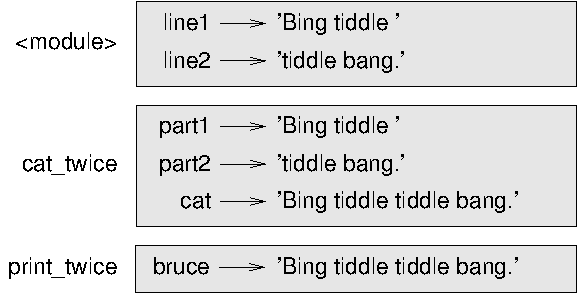
\includegraphics[scale=0.8]{figs/stack.pdf}}
\caption{Stack diagram.}
\label{fig.stack}
\end{figure}


The frames are arranged in a stack that indicates which function
called which, and so on.  In this example, \verb"print_twice"
was called by \verb"cat_twice", and \verb"cat_twice" was called by 
\verb"__main__", which is a special name for the topmost frame.  When
you create a variable outside of any function, it belongs to 
\verb"__main__".

栈里面的框架指出哪个函数被哪个函数调用等。
在此例中,\verb"print_twice"被\verb"cat_twice"调用,
\verb"cat_twice"被\verb"__main__"调用,这是一个表示最上层框架的特殊的名字。
当你在所有函数之外生成一个变量时,它属于\verb"__main__"。

Each parameter refers to the same value as its corresponding
argument.  So, {\tt part1} has the same value as
{\tt line1}, {\tt part2} has the same value as {\tt line2},
and {\tt bruce} has the same value as {\tt cat}.

每个形参都指向其相应的实参的值。
因此{\tt part1}和{\tt line1}的值相同,{\tt part2}和{\tt line2}的值相同,
{\tt bruce}和 {\tt cat}的值相同。

If an error occurs during a function call, Python prints the
name of the function, and the name of the function that called
it, and the name of the function that called {\em that}, all the
way back to \verb"__main__".

如果函数调用时发生错误,Python打印此函数的名字以及调用它的函数的名字,
以及那个调用的函数的名字,所有回到\verb"__main__"的路径。

For example, if you try to access {\tt cat} from within 
\verb"print_twice", you get a {\tt NameError}:

例如,如果你在\verb"print_twice"里面试图访问{\tt cat},
你获得一个{\tt NameError}:

\begin{verbatim}
Traceback (innermost last):
  File "test.py", line 13, in __main__
    cat_twice(line1, line2)
  File "test.py", line 5, in cat_twice
    print_twice(cat)
  File "test.py", line 9, in print_twice
    print cat
NameError: name 'cat' is not defined
\end{verbatim}
%
This list of functions is called a {\bf traceback}.  It tells you what
program file the error occurred in, and what line, and what functions
were executing at the time.  It also shows the line of code that
caused the error.
\index{traceback}

这个函数列表被称作一个{\bf 回溯(traceback)}。
它告诉你发生错误的程序文件,以及此时执行到哪一行,哪个函数。
它也展示引起错误的代码行。

The order of the functions in the traceback is the same as the
order of the frames in the stack diagram.  The function that is
currently running is at the bottom.


\section{Fruitful functions and void functions 有返回值函数和无返回值函数}
\index{fruitful function}
\index{void function}
\index{function, fruitful}
\index{function, void} 

Some of the functions we are using, such as the math functions, yield
results; for lack of a better name, I call them {\bf fruitful
  functions}.  Other functions, like \verb"print_twice", perform an
action but don't return a value.  They are called {\bf void
  functions}.
  
有一些我们正在用的函数,例如数学函数,会产生结果;
由于没有更好地命名,我叫它们{\bf 有返回值函数(fruitful functions)}。
其它的函数,像\verb"print_twice",执行一个动作但是不返回一个值。
它们被称为{\bf 无返回值函数(void functions)}。

When you call a fruitful function, you almost always
want to do something with the result; for example, you might
assign it to a variable or use it as part of an expression:

当你调用一个有返回值函数时,你几乎总是想用结果做些事情,
例如你可能将它赋给一个变量或者把它作为一个表达式的一部分。

\begin{verbatim}
x = math.cos(radians)
golden = (math.sqrt(5) + 1) / 2
\end{verbatim}
%
When you call a function in interactive mode, Python displays
the result:

当你在交互模式下调用一个函数的时候,Python显示结果:

\begin{verbatim}
>>> math.sqrt(5)
2.2360679774997898
\end{verbatim}
%
But in a script, if you call a fruitful function all by itself,
the return value is lost forever!

但是在脚本中,如果你只调用一个有返回值函数,
返回值永远就丢失了!

\begin{verbatim}
math.sqrt(5)
\end{verbatim}
%
This script computes the square root of 5, but since it doesn't store
or display the result, it is not very useful.
\index{interactive mode}
\index{script mode}

该脚本计算5的平方根,但是既然它没保存或者显示这个结果,
它不是非常有用。

Void functions might display something on the screen or have some
other effect, but they don't have a return value.  If you try to
assign the result to a variable, you get a special value called
{\tt None}.
\index{None special value}
\index{special value!None}

无返回值函数可能在屏幕上显示一些东西或者有些其它的影响,
但是它们没有返回值。如果你试图将这个结果赋给一个变量,
你获得一个特殊的被称作{\tt None}的值。

\begin{verbatim}
>>> result = print_twice('Bing')
Bing
Bing
>>> print result
None
\end{verbatim}
%
The value {\tt None} is not the same as the string \verb"'None'". 
It is a special value that has its own type:

值{\tt None}和字符串\verb"'None'"不同。这是一个有它自己的类型的特殊变量:

\begin{verbatim}
>>> print type(None)
<type 'NoneType'>
\end{verbatim}
%
The functions we have written so far are all void.  We will start
writing fruitful functions in a few chapters.

目前为止我们写的函数都是无返回值函数。
我们将在几章之后开始写有返回值函数。


\section{Why functions? 为什么用函数?}
\index{function, reasons for}

It may not be clear why it is worth the trouble to divide
a program into functions.  There are several reasons:

为什么值得麻烦地将一个程序分解成函数可能还不是很清楚。
有几个原因:

\begin{itemize}

\item Creating a new function gives you an opportunity to name a group
of statements, which makes your program easier to read and debug.

生成一个新的函数给你一个命名一组语句的机会,
这使得你的程序更容易读和调试。

\item Functions can make a program smaller by eliminating repetitive
code.  Later, if you make a change, you only have
to make it in one place.

通过避免重复调用代码,函数使得程序更小。
之后,如果你要做个变动,你只需在一处变动即可。

\item Dividing a long program into functions allows you to debug the
parts one at a time and then assemble them into a working whole.

将一个长程序分解为函数允许你一次调试一部分然后将它们集成为一个可行的整体。

\item Well-designed functions are often useful for many programs.
Once you write and debug one, you can reuse it.

良好设计的函数经常对多个程序都有用。一旦你写出并调试了一个函数,你可以重用它。

\end{itemize}


\section{Importing with {\tt from} 使用{\tt from}导入}

Python provides two ways to import modules; we have already seen one:

Python提供两种方法导入模块。我们已经看到了一种:

\begin{verbatim}
>>> import math
>>> print math
<module 'math' (built-in)>
>>> print math.pi
3.14159265359
\end{verbatim}
%
If you import {\tt math}, you get a module object named {\tt math}.
The module object contains constants like {\tt pi} and functions
like {\tt sin} and {\tt exp}.

如果你导入{\tt math},你获得一个名为{\tt math}的模块对象。
该模块对象包括类似{\tt pi}的常量以及类似{\tt sin}和{\tt exp}的函数。

But if you try to access {\tt pi} directly, you get an error.

但是,如果你试图直接访问{\tt pi},会获得一个错误:

\begin{verbatim}
>>> print pi
Traceback (most recent call last):
  File "<stdin>", line 1, in <module>
NameError: name 'pi' is not defined
\end{verbatim}
%
As an alternative, you can import an object from a module like this:

另一种方法是,你可以像这样从一个模块中导入一个对象:

\begin{verbatim}
>>> from math import pi
\end{verbatim}
%
Now you can access {\tt pi} directly, without dot notation.
\index{dot notation}

现在,你可以直接访问{\tt pi},不需要点记法了。

\begin{verbatim}
>>> print pi
3.14159265359
\end{verbatim}
%
Or you can use the star operator to import {\it everything} from the
module:

或者你可以用星号运算符从模块中导入所有的东西:

\begin{verbatim}
>>> from math import *
>>> cos(pi)
-1.0
\end{verbatim}

The advantage of importing everything from the math module is that your
code can be more concise.  The disadvantage is that there might be
conflicts between names defined in different modules, or between
a name from a module and one of your variables.

从数学模块中导入所有东西的优点是你的代码变得更简洁。
缺点是不同模块之间的名字,或者来自模块的名与你自己的变量名可能会冲突。


\section{Debugging 调试}
\label{editor}
\index{debugging}

If you are using a text editor to write your scripts, you might
run into problems with spaces and tabs.  The best way to avoid
these problems is to use spaces exclusively (no tabs).  Most text
editors that know about Python do this by default, but some
don't.
\index{whitespace}

如果你正在用一个文本编辑器写你的脚本,你可能会遇到空格和制表符的问题。
避免这些问题最好的办法是只使用空格(不用制表符)。
大多数识别Python的文本编辑器默认这么做,但有些不是。

Tabs and spaces are usually invisible, which makes them
hard to debug, so try to find an editor that manages indentation
for you.

制表符和空格通常是不可见的,这使得它们很难调试,
因此尽量找一个自动缩进的编辑器。

Also, don't forget to save your program before you run it.  Some
development environments do this automatically, but some don't.
In that case the program you are looking at in the text editor
is not the same as the program you are running.

同时,别忘了在运行程序之前保存它。
一些开发环境自动做这个,但是有些不是。
如果是这样的话,你在文本编辑器上看到的程序和你运行的不一样。

Debugging can take a long time if you keep running the same,
incorrect, program over and over!

如果你一遍一遍运行一个相同的、错误的程序,调试可能要花很长时间。

Make sure that the code you are looking at is the code you are running.
If you're not sure, put something like \verb"print 'hello'" at the
beginning of the program and run it again.  If you don't see
\verb"hello", you're not running the right program!

确定你所看到的代码是你所运行的。
如果不确定,将一些类似\verb"print 'hello'"的代码放到程序的开始并再次运行它。
如果你么有看到\verb"hello",那么你没在运行一个正确的程序。


\section{Glossary 术语表}

\begin{description}

\item[function(函数):] A named sequence of statements that performs some
useful operation.  Functions may or may not take arguments and may or
may not produce a result.
\index{function}

\item[function definition(函数定义):]  A statement that creates a new function,
specifying its name, parameters, and the statements it executes.
\index{function definition}

\item[function object(函数对象):]  A value created by a function definition.
The name of the function is a variable that refers to a function
object.
\index{function definition}

\item[header(函数头):] The first line of a function definition.
\index{header}

\item[body(函数体):] The sequence of statements inside a function definition.
\index{body}

\item[parameter(形参):] A name used inside a function to refer to the value
passed as an argument.
\index{parameter}

\item[function call(函数调用):] A statement that executes a function. It
consists of the function name followed by an argument list.
\index{function call}

\item[argument(实参):]  A value provided to a function when the function is called.
This value is assigned to the corresponding parameter in the function.
\index{argument}

\item[local variable(局部变量):]  A variable defined inside a function.  A local
variable can only be used inside its function.
\index{local variable}

\item[return value(返回值):]  The result of a function.  If a function call
is used as an expression, the return value is the value of
the expression.
\index{return value}

\item[fruitful function(有返回值函数):] A function that returns a value.
\index{fruitful function}

\item[void function(无返回值函数):] A function that doesn't return a value.
\index{void function}

\item[module(模块):] A file that contains a
collection of related functions and other definitions.
\index{module}

\item[import statement(导入语句):] A statement that reads a module file and creates
a module object.
\index{import statement}
\index{statement!import}

\item[module object(模块对象):] A value created by an {\tt import} statement
that provides access to the values defined in a module.
\index{module}

\item[dot notation(点记法):]  The syntax for calling a function in another
module by specifying the module name followed by a dot (period) and
the function name.
\index{dot notation}

\item[composition(组合):] Using an expression as part of a larger expression,
or a statement as part of a larger statement.
\index{composition}

\item[flow of execution(执行流程):]  The order in which statements are executed during
a program run.
\index{flow of execution}

\item[stack diagram(栈图):]  A graphical representation of a stack of functions,
their variables, and the values they refer to.
\index{stack diagram}

\item[frame(框架):]  A box in a stack diagram that represents a function call.
It contains the local variables and parameters of the function.
\index{function frame}
\index{frame}

\item[traceback(回溯):]  A list of the functions that are executing,
printed when an exception occurs.
\index{traceback}


\end{description}


\section{Exercises}

\begin{exercise}
\index{len function}
\index{function!len}

Python provides a built-in function called {\tt len} that
returns the length of a string, so the value of \verb"len('allen')" is 5.

Write a function named \verb"right_justify" that takes a string
named {\tt s} as a parameter and prints the string with enough
leading spaces so that the last letter of the string is in column 70
of the display.

\begin{verbatim}
>>> right_justify('allen')
                                                                 allen
\end{verbatim}

\end{exercise}


\begin{exercise}
\index{function object}
\index{object!function}

A function object is a value you can assign to a variable
or pass as an argument.  For example, \verb"do_twice" is a function
that takes a function object as an argument and calls it twice:

\begin{verbatim}
def do_twice(f):
    f()
    f()
\end{verbatim}

Here's an example that uses \verb"do_twice" to call a function
named \verb"print_spam" twice.

\begin{verbatim}
def print_spam():
    print 'spam'

do_twice(print_spam)
\end{verbatim}

\begin{enumerate}

\item Type this example into a script and test it.

\item Modify \verb"do_twice" so that it takes two arguments, a
function object and a value, and calls the function twice,
passing the value as an argument.

\item Write a more general version of \verb"print_spam", called
\verb"print_twice", that takes a string as a parameter and prints
it twice.

\item Use the modified version of \verb"do_twice" to call
\verb"print_twice" twice, passing \verb"'spam'" as an argument.

\item Define a new function called 
\verb"do_four" that takes a function object and a value
and calls the function four times, passing the value
as a parameter.  There should be only
two statements in the body of this function, not four.

\end{enumerate}

Solution: \url{http://thinkpython.com/code/do_four.py}.

\end{exercise}



\begin{exercise}

This exercise can be
done using only the statements and other features we have learned so
far.  

\begin{enumerate}

\item Write a function that draws a grid like the following:
\index{grid}

\begin{verbatim}
+ - - - - + - - - - +
|         |         |
|         |         |
|         |         |
|         |         |
+ - - - - + - - - - +
|         |         |
|         |         |
|         |         |
|         |         |
+ - - - - + - - - - +
\end{verbatim}
%
Hint: to print more than one value on a line, you can print
a comma-separated sequence:

\begin{verbatim}
print '+', '-'
\end{verbatim}
%
If the sequence ends with a comma, Python leaves the line unfinished,
so the value printed next appears on the same line.

\begin{verbatim}
print '+', 
print '-'
\end{verbatim}
%
The output of these statements is \verb"'+ -'".

A {\tt print} statement all by itself ends the current line and
goes to the next line.

\item Write a function that draws a similar grid
with four rows and four columns.

\end{enumerate}

Solution: \url{http://thinkpython.com/code/grid.py}.
Credit: This exercise is based on an exercise in Oualline, {\em
    Practical C Programming, Third Edition}, O'Reilly Media, 1997.
\end{exercise}
\chapter{Case study: interface design 案例学习:接口设计}
\label{turtlechap}
Code examples from this chapter are available from
\url{http://thinkpython.com/code/polygon.py}.
本章的示例代码可以从\url{http://thinkpython.com/code/polygon.py}获得。
\section{TurtleWorld}
\index{TurtleWorld}
\index{Swampy}

To accompany this book, I have written a package called Swampy.
You can download Swampy from \url{http://thinkpython.com/swampy};
follow the instructions there to install Swampy on your system.

作为对本书的补充,我写了一个叫Swampy的包。
你可以从\url{http://thinkpython.com/swampy}下载Swampy,
然后按照说明在你的系统上安装Swampy。

A {\bf package} is a collection of modules; one of the modules in
Swampy is {\tt TurtleWorld}, which provides a set of functions for
drawing lines by steering turtles around the screen.
\index{package}

一个{\bf 包(package)}是一套模块,{\tt TurtleWorld}是Swampy中的一个模块,
其提供了一组通过在屏幕上转向海龟的画线函数。
 
If Swampy is installed as a package on your system, you can import
{\tt TurtleWorld} like this:

如果Swampy作为包被安装在了你的系统上,你可以像这样导入{\tt TurtleWorld}:

\begin{verbatim}
from swampy.TurtleWorld import *
\end{verbatim}

If you downloaded the Swampy modules but did not install them as a
package, you can either work in the directory that contains the Swampy
files, or add that directory to Python's search path.  Then you can import
{\tt TurtleWorld} like this:

如果你下载了Swampy模块但是没有作为包安装,
你要么可以在含有Swampy的文件夹里工作,或者将此目录增加到Python的搜索路径。
然后你可以像这样导入{\tt TurtleWorld}:

\begin{verbatim}
from TurtleWorld import *
\end{verbatim}

The details of the installation process and setting Python's search
path depend on your system, so rather than include those details here,
I will try to maintain current information for several systems
at \url{http://thinkpython.com/swampy}.

安装和设置Python搜索路径的细节依赖于你的系统,
所以我不在此包括那些细节了,
我将试着在\url{http://thinkpython.com/swampy}维护多个系统的最新的信息。

Create a file named {\tt mypolygon.py} and type in the following
code:

生成一个叫{\tt mypolygon.py}的文件并键入如下代码:

\begin{verbatim}
from swampy.TurtleWorld import *

world = TurtleWorld()
bob = Turtle()
print bob

wait_for_user()
\end{verbatim}
%
The first line imports everything from the {\tt TurtleWorld} module
in the {\tt swampy} package.
\index{import statement}
\index{statement!import}

第一行在{\tt swampy}里从{\tt TurtleWorld}模块导入内容。

The next lines create a TurtleWorld assigned to {\tt world} and
a Turtle assigned to {\tt bob}.  Printing {\tt bob} yields something
like:

接下来几行生成一个TurtleWorld赋给{\tt world}以及生成一个Turtle赋给{\tt bob}。
打印{\tt bob}产生像下面这样的东西:

\begin{verbatim}
<TurtleWorld.Turtle instance at 0xb7bfbf4c>
\end{verbatim}
%
This means that {\tt bob} refers to
an {\bf instance} of a Turtle
as defined in module {\tt TurtleWorld}.  In this context,
``instance'' means a member of a set;
this Turtle is one of the set of possible Turtles.
\index{instance}

这意味着{\tt bob}指向一个如{\tt TurtleWorld}中定义的Turtle的{\bf 实例(instance)}。
在此处,``实例''的意思是集合的一个成员,该Turtle是所有可能的Turtle构成的集合的一个元素。

\verb"wait_for_user" tells TurtleWorld to wait for the user
to do something, although in this case there's not much for
the user to do except close the window.

\verb"wait_for_user"告诉TurtleWorld等待用户做些什么,
但是在此例中除了关闭窗口外用户也做不了其它的事情。

TurtleWorld provides several
turtle-steering functions: {\tt fd} and {\tt bk} for
forward and backward, and {\tt lt} and {\tt rt} for left and
right turns.  Also, each Turtle is holding a pen, which is
either down or up; if the pen is down, the Turtle leaves
a trail when it moves.  The functions {\tt pu} and {\tt pd}
stand for ``pen up'' and ``pen down''.

TurtleWorld提供几个海龟转向函数:
{\tt fd}和{\tt bk}用于向前和向后,{\tt lt}和{\tt rt}是向左和向右。
每个海龟都握有一支笔,要么放下,要么抬起。
如果笔被放下,该海龟留下它走过的痕迹。
函数{\tt pu}和{\tt pd}代表``笔抬起''和``笔放下''。

To draw a right angle, add these lines to the program
(after creating {\tt bob} and before calling \verb"wait_for_user"):

为了画一个向右的三角,在程序中加入这些代码
(在生成{\tt bob}之后,调用\verb"wait_for_user"之前):

\begin{verbatim}
fd(bob, 100)
lt(bob)
fd(bob, 100)
\end{verbatim}
%
The first line tells {\tt bob} to take 100 steps
forward.  The second line tells him to turn left.

第一行告诉{\tt bob}向前走100步。第二行告诉它向左转。

When you run this program, you should see {\tt bob} move east and then
north, leaving two line segments behind.

当运行此程序时,你应该会看见{\tt bob}现象东移动,然后向北,
在它后面留下两条线段。

Now modify the program to draw a square.  Don't go on until
you've got it working!

现在修改程序画一个正方形。如果没有成功,不要继续往下读。

%\newpage

\section{Simple repetition 简单的重复}
\label{repetition}
\index{repetition}

Chances are you wrote something like this (leaving out the code
that creates TurtleWorld and waits for the user):

假设你写了如下的代码(不包括生成TurtleWorld以及等待用户的代码):

\begin{verbatim}
fd(bob, 100)
lt(bob)

fd(bob, 100)
lt(bob)

fd(bob, 100)
lt(bob)

fd(bob, 100)
\end{verbatim}
%
We can do the same thing more concisely with a {\tt for} statement.
Add this example to {\tt mypolygon.py} and run it again:
\index{for loop}
\index{loop!for}
\index{statement!for}

我们可以用更简洁的{\tt for}语句做相同的事情。
将这个示例加入{\tt mypolygon.py}并重新运行它:

\begin{verbatim}
for i in range(4):
    print 'Hello!'
\end{verbatim}
%
You should see something like this:

你会看到如下内容:

\begin{verbatim}
Hello!
Hello!
Hello!
Hello!
\end{verbatim}
%
This is the simplest use of the {\tt for} statement; we will see
more later.  But that should be enough to let you rewrite your
square-drawing program.  Don't go on until you do.

这是{\tt for}语句最简单的用法,后面我们会看到更多的。
但是这对于你重写你的画正方形程序已经足够了。
如果没有完成不要继续。

Here is a {\tt for} statement that draws a square:

下面是使用{\tt for}语句画正方形:

\begin{verbatim}
for i in range(4):
    fd(bob, 100)
    lt(bob)
\end{verbatim}
%
The syntax of a {\tt for} statement is similar to a function
definition.  It has a header that ends with a colon and an indented
body.  The body can contain any number of statements.
\index{loop}

{\tt for}语句的语法和函数定义类似。
它有一个以冒号结尾的头以及一个缩进的体。
体可以包含任意条数的语句。

A {\tt for} statement is sometimes called a {\bf loop} because
the flow of execution runs through the body and then loops back
to the top.  In this case, it runs the body four times.

{\tt for}语句有时被称为{\bf 循环(loop)},因为执行流程运行整个体然后循环回顶部。
在此例中,它运行体4次。

This version is actually a little different from the previous
square-drawing code because it makes another turn after
drawing the last side of the square.  The extra turn takes a little
more time, but it simplifies the code if we do the same thing
every time through the loop.  This version also has the effect
of leaving the turtle back in the starting position, facing in
the starting direction.

此版本和前面画正方形的代码有所不同,因为它在画完正方形最后一条边的时候,
又多转了一下。这个额外的转动多花了些时间,
但是如果我们通过循环做相同的事情也简化了代码。
此版本也有一个作用,将海龟留在了出发位置,朝向开始的方向。

\section{Exercises 练习}

The following is a series of exercises using TurtleWorld.  They
are meant to be fun, but they have a point, too.  While you are
working on them, think about what the point is.

下面是一系列使用TurtleWorld的练习。
它们是很有趣,但是它们也都有一点。
当你做这些练习的时候,想一想这个点是什么?

The following sections have solutions to the exercises, so
don't look until you have finished (or at least tried).

下面几节是这些练习的答案,因此如果你没完成(或者至少试过了),不要看答案。

\begin{enumerate}

\item Write a function called {\tt square} that takes a parameter
named {\tt t}, which is a turtle.  It should use the turtle to draw
a square.

写一个名为{\tt square}的函数,有一个名为{\tt t}的形参,它是一个海龟。
用这只海龟画一个正方形。

Write a function call that passes {\tt bob} as an argument to
{\tt square}, and then run the program again.

写一个函数调用,将{\tt bob}作为实参传给{\tt square},然后再重新运行程序。

\item Add another parameter, named {\tt length}, to {\tt square}.
Modify the body so length of the sides is {\tt length}, and then
modify the function call to provide a second argument.  Run the
program again.  Test your program with a range of values for {\tt
length}.

给{\tt square}加入另一个名为{\tt length}的形参。
修改函数体,使得边的长度是{\tt square},然后修改函数调用以提供第二个实参。
重新运行程序。用一个范围内的{\tt length}值测试你的程序。

\item The functions {\tt lt} and {\tt rt} make 90-degree turns by
default, but you can provide a second argument that specifies the
number of degrees.  For example, {\tt lt(bob, 45)} turns {\tt bob} 45
degrees to the left.

函数{\tt lt}和{\tt rt}默认转动90度,而你可以提供第二个实参来制定角度。
例如{\tt lt(bob, 45)}向左转动{\tt bob} 45度。

Make a copy of {\tt square} and change the name to {\tt polygon}.  Add
another parameter named {\tt n} and modify the body so it draws an
n-sided regular polygon.  Hint: The exterior angles of an n-sided regular
polygon are $360/n$ degrees.
\index{polygon function}
\index{function!polygon}

复制{\tt square}并改名为{\tt polygon}。
增加另外一个名为{\tt n}的参数并改变函数体,让它画一个n边形。
提示:n边型的外角是$360/n$度。

\item Write a function called {\tt circle} that takes a turtle, {\tt t},
and radius, {\tt r}, as parameters and that draws an approximate circle
by invoking {\tt polygon} with an appropriate length and number of
sides.  Test your function with a range of values of {\tt r}.
\index{circle function}
\index{function!circle}

写一个名为{\tt circle}的函数,它接受一个乌龟{\tt t}和半径{\tt r}作为形参,
然后通过调用{\tt polygon},用合适的边的数目和长度画一个近似圆形。
用一定范围内的{\tt r}值测试你的函数。

Hint: figure out the circumference of the circle and make sure that
{\tt length * n = circumference}.

提示:指出圆的周长并确定{\tt length * n = circumference}。

Another hint: if {\tt bob} is too slow for you, you can speed
him up by changing {\tt bob.delay}, which is the time between moves,
in seconds.  {\tt bob.delay = 0.01} ought to get him moving.

另外一个提示:如果{\tt bob}对你来说太慢了,你可以通过修改{\tt bob.delay}加速,
它是两次移动之间的时间(秒)。{\tt bob.delay = 0.01}应该让它移动。

% change this to world.delay

\item Make a more general version of {\tt circle} called {\tt arc}
that takes an additional parameter {\tt angle}, which determines
what fraction of a circle to draw.  {\tt angle} is in units of
degrees, so when {\tt angle=360}, {\tt arc} should draw a complete
circle.
\index{arc function}
\index{function!arc}

完成一个更一般的{\tt circle}版本{\tt arc},其接受一个额外的参数{\tt angle},
确定画多大部分的圆。{\tt angle}的单位是度,因此当{\tt angle=360}时,
{\tt arc} 应该画一个整圆。

\end{enumerate}

\section{Encapsulation 封装}

The first exercise asks you to put your square-drawing code
into a function definition and then call the function, passing
the turtle as a parameter.  Here is a solution:

第一个练习需要你将画正方形的代码放到函数定义中然后调用该函数,
传递海龟作为参数。这是答案:

\begin{verbatim}
def square(t):
    for i in range(4):
        fd(t, 100)
        lt(t)

square(bob)
\end{verbatim}
%
The innermost statements, {\tt fd} and {\tt lt} are
indented twice to show that they are inside the {\tt for} loop,
which is inside the function definition.  The next line,
{\tt square(bob)}, is flush with the left margin, so that is the
end of both the {\tt for} loop and the function definition.

最内部的语句,{\tt fd}和{\tt lt}缩进两次以显示它们在{\tt for}循环内,
该循环在函数内。下一行{\tt square(bob)}和左边界对齐,
因此它是{\tt for}循环和函数定义的结束。

Inside the function, {\tt t} refers to the same turtle {\tt bob}
refers to, so {\tt lt(t)} has the same effect as {\tt lt(bob)}.
So why not call the parameter {\tt bob}?  The idea is that {\tt t}
can be any turtle, not just {\tt bob}, so you could create
a second turtle and pass it as an argument to {\tt square}:

在函数内部,{\tt t}和{\tt bob}指的是同一只海龟,
所以{\tt lt(t)}和{\tt lt(bob)}功能相同。
那么为什么不将形参命名为{\tt bob}呢?
想法是{\tt t}可以是任何海龟而不仅仅是{\tt bob},
所以你可以生成第二只海龟并且将它作为实参传递给{\tt square}:

\begin{verbatim}
ray = Turtle()
square(ray)
\end{verbatim}
%
Wrapping a piece of code up in a function is called {\bf
encapsulation}.  One of the benefits of encapsulation is that it
attaches a name to the code, which serves as a kind of documentation.
Another advantage is that if you re-use the code, it is more concise
to call a function twice than to copy and paste the body!
\index{encapsulation}

将一部分代码包装在函数里被称作 {\bf encapsulation(封装)}。
封装的好处之一是它将这些代码赋予一个名字,
这充当了一种文档。另一个好处是你可以重用这些代码,
调用函数两次要比拷贝粘贴函数体要简洁!

\section{Generalization 泛化}

The next step is to add a {\tt length} parameter to {\tt square}.
Here is a solution:

下一步是给{\tt square}增加一个{\tt length}形参。这是解决方案:

\begin{verbatim}
def square(t, length):
    for i in range(4):
        fd(t, length)
        lt(t)

square(bob, 100)
\end{verbatim}
%
Adding a parameter to a function is called {\bf generalization}
because it makes the function more general: in the previous
version, the square is always the same size; in this version
it can be any size.
\index{generalization}

为函数增加一个形参被称作{\bf 泛化(generalization)},
因为其使得函数更一般:在前面的版本中,
正方形总是相同大小的;此版本它可以是任意的大小。

The next step is also a generalization.  Instead of drawing
squares, {\tt polygon} draws regular polygons with any number of
sides.  Here is a solution:

下一步也是一个泛化。不是画一个正方形,{\tt polygon}画任意的多边形。
这是解决方案:

\begin{verbatim}
def polygon(t, n, length):
    angle = 360.0 / n
    for i in range(n):
        fd(t, length)
        lt(t, angle)

polygon(bob, 7, 70)
\end{verbatim}
%
This draws a 7-sided polygon with side length 70.  If you have
more than a few numeric arguments, it is easy to forget what they
are, or what order they should be in.  It is legal, and sometimes
helpful, to include the names of the parameters in the argument
list:

这画了一个7边形,边长为70。
如果你有更多的形参,很容易忘记它们多是什么或者它们的顺序应该是什么。
将形参名放入实参列表是合法的,而且有时很有用:

\begin{verbatim}
polygon(bob, n=7, length=70)
\end{verbatim}
%
These are called {\bf keyword arguments} because they include
the parameter names as ``keywords'' (not to be confused with
Python keywords like {\tt while} and {\tt def}).
\index{keyword argument}
\index{argument!keyword}

这些被称作{\bf 关键字实参(keyword arguments)},
因为它们包含了形参名作为``关键字''(不要和Python的关键字搞混了,如{\tt while}和{\tt def})。

This syntax makes the program more readable.  It is also a reminder
about how arguments and parameters work: when you call a function, the
arguments are assigned to the parameters.

这一语法使得程序更可读。
它也是关于实参和形参如何工作的一个提醒:
当你调用函数时,实参被赋给形参。


\section{Interface design 接口设计}

The next step is to write {\tt circle}, which takes a radius,
{\tt r}, as a parameter.  Here is a simple solution that uses
{\tt polygon} to draw a 50-sided polygon:

下一步是写{\tt circle},它将半径{\tt r}作为形参。
这是一个简单的解决方案,它使用{\tt polygon}画一个50边形:

\begin{verbatim}
def circle(t, r):
    circumference = 2 * math.pi * r
    n = 50
    length = circumference / n
    polygon(t, n, length)
\end{verbatim}
%
The first line computes the circumference of a circle with radius
{\tt r} using the formula $2 \pi r$.  Since we use {\tt math.pi}, we
have to import {\tt math}.  By convention, {\tt import} statements
are usually at the beginning of the script.

第一行用半径{\tt r}计算圆的周长,公式是$2 \pi r$。
由于我们用了{\tt math.pi},我们需要导入{\tt math}。
按照惯例,{\tt import}语句通常位于脚本开始。

{\tt n} is the number of line segments in our approximation of a circle,
so {\tt length} is the length of each segment.  Thus, {\tt polygon}
draws a 50-sides polygon that approximates a circle with radius {\tt r}.

{\tt n}是我们估计的圆的线段的个数,所以{\tt length}是每一段的长度。
这样{\tt polygon}画一个50边形来估计一个半径为{\tt r}的圆。

One limitation of this solution is that {\tt n} is a constant, which
means that for very big circles, the line segments are too long, and
for small circles, we waste time drawing very small segments.  One
solution would be to generalize the function by taking {\tt n} as
a parameter.  This would give the user (whoever calls {\tt circle})
more control, but the interface would be less clean.
\index{interface}

这种解决方案的一个局限性是{\tt n}是常数,这意味着对于非常大的圆,
线段会非常长,并且对于小圆,我们浪费时间画非常小的线段。
一个解决方案是通过将{\tt n}作为形参来泛化函数。
这将给用户(调用{\tt circle}的人)更多的控制,
但是接口将不那么干净了。

The {\bf interface} of a function is a summary of how it is used: what
are the parameters?  What does the function do?  And what is the return
value?  An interface is ``clean'' if it is ``as simple as
possible, but not simpler. (Einstein)''
\index{Einstein, Albert}

函数的{\bf 接口(interface)}是一个如何使用它的摘要:
形参是什么?函数做什么?返回值是什么?
如果接口``尽可能简单,但不能过于简单(爱因斯坦)''的话,则说它是``干净的''。

In this example, {\tt r} belongs in the interface because it
specifies the circle to be drawn.  {\tt n} is less appropriate
because it pertains to the details of {\em how} the circle should
be rendered.

在这个例子中,{\tt r}属于接口,因为它确定了被画的圆。
{\tt n}就不太合适,因为他是关于如何画圆的细节。

Rather than clutter up the interface, it is better
to choose an appropriate value of {\tt n}
depending on {\tt circumference}:

不要把接口弄乱,依赖{\tt circumference}选择一个合适的{\tt n}值比较好。

\begin{verbatim}
def circle(t, r):
    circumference = 2 * math.pi * r
    n = int(circumference / 3) + 1
    length = circumference / n
    polygon(t, n, length)
\end{verbatim}
%
Now the number of segments is (approximately) {\tt circumference/3},
so the length of each segment is (approximately) 3, which is small
enough that the circles look good, but big enough to be efficient,
and appropriate for any size circle.

现在线段的数量(大概)是{\tt circumference/3},
所以每条线段的长度(大概)是3,这足够的小了,
使得圆看上去不错,但是对于保证效率也足够大了,
适合任何大小的圆。

\section{Refactoring 重构}
\label{refactoring}
\index{refactoring}

When I wrote {\tt circle}, I was able to re-use {\tt polygon}
because a many-sided polygon is a good approximation of a circle.
But {\tt arc} is not as cooperative; we can't use {\tt polygon}
or {\tt circle} to draw an arc.

当我写{\tt circle}的时候,我能够重用{\tt polygon},
因为一个多边形是对圆的很好的近似。
但是{\tt arc}不太易于合作,我们不能使用{\tt polygon}或者{\tt circle}来画一个弧。

One alternative is to start with a copy
of {\tt polygon} and transform it into {\tt arc}.  The result
might look like this:

一种替代方案是从{\tt polygon}的一个拷贝开始,
并将它转化为{\tt arc}。结果看上去像这样:

\begin{verbatim}
def arc(t, r, angle):
    arc_length = 2 * math.pi * r * angle / 360
    n = int(arc_length / 3) + 1
    step_length = arc_length / n
    step_angle = float(angle) / n
    
    for i in range(n):
        fd(t, step_length)
        lt(t, step_angle)
\end{verbatim}
%
The second half of this function looks like {\tt polygon}, but we
can't re-use {\tt polygon} without changing the interface.  We could
generalize {\tt polygon} to take an angle as a third argument,
but then {\tt polygon} would no longer be an appropriate name!
Instead, let's call the more general function {\tt polyline}:

该函数的后半部分看上去很像{\tt polygon},
但是在不改变接口的条件下我们不能重用{\tt polygon}。
我们可以泛化{\tt polygon}来接受一个角度作为第三个实参,
但是这样{\tt polygon}就不再是一个合适的名字了!
让我们称这个更一般的函数为{\tt polyline}:

\begin{verbatim}
def polyline(t, n, length, angle):
    for i in range(n):
        fd(t, length)
        lt(t, angle)
\end{verbatim}
%
Now we can rewrite {\tt polygon} and {\tt arc} to use {\tt polyline}:
现在,我们可以用{\tt polyline}重写{\tt polygon}和{\tt arc}:

\begin{verbatim}
def polygon(t, n, length):
    angle = 360.0 / n
    polyline(t, n, length, angle)

def arc(t, r, angle):
    arc_length = 2 * math.pi * r * angle / 360
    n = int(arc_length / 3) + 1
    step_length = arc_length / n
    step_angle = float(angle) / n
    polyline(t, n, step_length, step_angle)
\end{verbatim}
%
Finally, we can rewrite {\tt circle} to use {\tt arc}:
最后,我们可以用{\tt arc}重写{\tt circle}:

\begin{verbatim}
def circle(t, r):
    arc(t, r, 360)
\end{verbatim}
%
This process---rearranging a program to improve function
interfaces and facilitate code re-use---is called {\bf refactoring}.
In this case, we noticed that there was similar code in {\tt arc} and
{\tt polygon}, so we ``factored it out'' into {\tt polyline}.
\index{refactoring}

这个过程---重新整理一个程序以改进函数接口和促进代码的重用性---
被称作{\bf 重构(refactoring)}。
在此例中,我们注意到{\tt arc}和{\tt polygon}中有相似的代码,
因此,我们``将它分解出来''放入{\tt polyline}。

If we had planned ahead, we might have written {\tt polyline} first
and avoided refactoring, but often you don't know enough at the
beginning of a project to design all the interfaces.  Once you start
coding, you understand the problem better.  Sometimes refactoring is a
sign that you have learned something.

如果我们提前已经计划好了,我们可能首先写{\tt polyline}并避免重构,
但是在一个项目开始的时候,你经常知道的不足,不能设计全部的接口。
一旦你开始编码,你更好地理解该问题。
有时重构是一个信号,说明你已经学到某些东西了。


\section{A development plan 开发方案}
\index{development plan!encapsulation and generalization}

A {\bf development plan} is a process for writing programs.
The process we used
in this case study is ``encapsulation and
generalization.''  The steps of this process are:

{\bf 开发方案(development plan)}是写程序的一个过程。
此例中我们使用的过程是``封装和泛化''。
此过程的步骤是:

\begin{enumerate}

\item Start by writing a small program with no function definitions.

从写一个没有函数定义的小程序开始。

\item Once you get the program working, encapsulate it in a function
and give it a name.

一旦该程序运转起来,将它封装进一个函数并给它一个名字。

\item Generalize the function by adding appropriate parameters.

通过增加适当的形参泛化该函数。

\item Repeat steps 1--3 until you have a set of working functions.
Copy and paste working code to avoid retyping (and re-debugging).

重复1--3步,直到你有一些可运转的函数。
拷贝和粘贴代码以避免重新键入(和重新调试)。

\item Look for opportunities to improve the program by refactoring.
For example, if you have similar code in several places, consider
factoring it into an appropriately general function.

寻找机会通过重构改进程序。
例如如果在多个地方有相似的代码,考虑将它分解到一个合适的函数中。

\end{enumerate}

This process has some drawbacks---we will see alternatives later---but
it can be useful if you don't know ahead of time how to divide the
program into functions.  This approach lets you design as you go
along.

这个过程有一些缺点---后面我们将看到替代方案---
但是如果你之前不知道如果将程序分解为函数,它可能很有用。
该方法让你一边编程,一边设计。


\section{docstring 文档字符串}
\label{docstring}
\index{docstring}

A {\bf docstring} is a string at the beginning of a function that
explains the interface (``doc'' is short for ``documentation'').  Here
is an example:

一个{\bf 文档字符串(docstring)}是位于函数开始的字符串,
其解释函数的接口(``doc''是``document''的缩写)。
这是一个例子:

\begin{verbatim}
def polyline(t, n, length, angle):
    """Draws n line segments with the given length and
    angle (in degrees) between them.  t is a turtle.
    """    
    for i in range(n):
        fd(t, length)
        lt(t, angle)
\end{verbatim}
%
This docstring is a triple-quoted string, also known
as a multiline string because the triple quotes allow the string
to span more than one line.
\index{quotation mark}
\index{triple-quoted string}
\index{string!triple-quoted}
\index{multiline string}
\index{string!multiline}

此文档字符串是一个三引号字符串,也被称为多行字符串,
因为三引号允许字符串超过一行。

It is terse, but it contains the essential information
someone would need to use this function.  It explains concisely what
the function does (without getting into the details of how it does
it).  It explains what effect each parameter has on the behavior of
the function and what type each parameter should be (if it is not
obvious).

它很简单,但是它包括了该函数的必要信息。
它简要的说明了该函数做什么(没有介绍它如何工作的细节)。
它说明了每个形参对函数的行为有什么作用以及每个形参应有的类型
(如果它并不明显)。

Writing this kind of documentation is an important part of interface
design.  A well-designed interface should be simple to explain;
if you are having a hard time explaining one of your functions,
that might be a sign that the interface could be improved.

写这种文档是接口设计很重要的部分。
一个良好设计的接口应该解释起来很简单,
如果你很难解释你的函数,这也许是该接口可能需要被改进的一个信号。


\section{Debugging 调试}
\index{debugging}
\index{interface}

An interface is like a contract between a function and a caller.
The caller agrees to provide certain parameters and the function
agrees to do certain work.

接口就像是函数和一个调用者之间的合同。
调用者同意提供某些参数,函数统一做某些工作。

For example, {\tt polyline} requires four arguments: {\tt t} has to be
a Turtle; {\tt n} is the number of line segments, so it has to be an
integer; {\tt length} should be a positive number; and {\tt
  angle} has to be a number, which is understood to be in degrees.
  
例如,{\tt polyline}需要4个实参:{\tt t}必须是一个Turtle;
{\tt n}是线段的个数,因此它必须是一个整数;
{\tt length}应该是一个正数;
{\tt angle}必须是一个数,它被理解为一个度数。

These requirements are called {\bf preconditions} because they
are supposed to be true before the function starts executing.
Conversely, conditions at the end of the function are
{\bf postconditions}.  Postconditions include the intended
effect of the function (like drawing line segments) and any
side effects (like moving the Turtle or making other changes
in the World).
\index{precondition}
\index{postcondition}

这些需求被称作{\bf 先决条件(preconditions)},
因为它们在函数开始执行之前被假设为正确的。
相反,函数结束时的条件是{\bf 后置条件(postconditions)}。
后置条件包括函数预期的效果(如画线段)以及任何侧面效果
(如移动Turtle或者World中的其它改变)。

Preconditions are the responsibility of the caller.  If the caller
violates a (properly documented!) precondition and the function
doesn't work correctly, the bug is in the caller, not the function.

先决条件是调用者的职责。如果调用者违反一个(恰当的说明)
先决条件并且函数不正确的工作,则错误在调用者中,而不是函数中。

% Removing this because we haven't seen conditionals yet!
%However, for purposes of debugging it is often a good idea for
%functions to check their preconditions rather than assume they are
%true.  If every function checks its preconditions before starting,
%then if something goes wrong, you will know which function to blame.


\section{Glossary 术语表}

\begin{description}

\item[instance (实例):] A member of a set.  The TurtleWorld in this
chapter is a member of the set of TurtleWorlds.
\index{instance}

\item[loop (循环):] A part of a program that can execute repeatedly.
\index{loop}

\item[encapsulation (封装):] The process of transforming a sequence of
statements into a function definition.
\index{encapsulation}

\item[generalization (泛化):] The process of replacing something
unnecessarily specific (like a number) with something appropriately
general (like a variable or parameter).
\index{generalization}

\item[keyword argument (关键字实参):] An argument that includes the name of
the parameter as a ``keyword.''
\index{keyword argument}
\index{argument!keyword}

\item[interface (接口):] A description of how to use a function, including
the name and descriptions of the arguments and return value.
\index{interface}

\item[refactoring (重构):] The process of modifying a working program to
  improve function interfaces and other qualities of the code.
\index{refactoring}

\item[development plan (开发方案):] A process for writing programs.
\index{development plan}

\item[docstring (文档字符串):]  A string that appears in a function definition
to document the function's interface.
\index{docstring}

\item[precondition (先决条件):] A requirement that should be satisfied by
the caller before a function starts.
\index{precondition}

\item[postcondition (后置条件):] A requirement that should be satisfied by
the function before it ends.
\index{postcondition}

\end{description}


\section{Exercises}

\begin{exercise}

Download the code in this chapter from
\url{http://thinkpython.com/code/polygon.py}.

\begin{enumerate}

\item Write appropriate docstrings for {\tt polygon}, {\tt arc} and
{\tt circle}.
\index{stack diagram}

\item Draw a stack diagram that shows the state of the program
while executing {\tt circle(bob, radius)}.  You can do the
arithmetic by hand or add {\tt print} statements to the code.

\item The version of {\tt arc} in Section~\ref{refactoring} is not
very accurate because the linear approximation of the
circle is always outside the true circle.  As a result,
the turtle ends up a few units away from the correct
destination. My solution shows a way to reduce
the effect of this error.  Read the code and see if it makes
sense to you.  If you draw a diagram, you might see how it works.

\end{enumerate}

\end{exercise}

\begin{figure}
\centerline
{
\includegraphics[scale=0.8]{figs/flowers.pdf}}
\caption{Turtle flowers.}
\label{fig.flowers}
\end{figure}

\begin{exercise}
\index{flower}

Write an appropriately general set of functions that
can draw flowers as in Figure~\ref{fig.flowers}.

Solution: \url{http://thinkpython.com/code/flower.py},
also requires \url{http://thinkpython.com/code/polygon.py}.

\end{exercise}

\begin{figure}
\centerline
{
\includegraphics[scale=0.8]{figs/pies.pdf}}
\caption{Turtle pies.}
\label{fig.pies}
\end{figure}


\begin{exercise}
\index{pie}

Write an appropriately general set of functions that
can draw shapes as in Figure~\ref{fig.pies}.

Solution: \url{http://thinkpython.com/code/pie.py}.

\end{exercise}

\begin{exercise}
\index{alphabet}
\index{turtle typewriter}
\index{typewriter, turtle}

The letters of the alphabet can be constructed from a moderate number
of basic elements, like vertical and horizontal lines and a few
curves.  Design a font that can be drawn with a minimal number of
basic elements and then write functions that draw letters of the
alphabet.

You should write one function for each letter, with names
\verb"draw_a", \verb"draw_b", etc., and put your functions
in a file named {\tt letters.py}.  You can download a
``turtle typewriter'' from \url{http://thinkpython.com/code/typewriter.py}
to help you test your code.

Solution: \url{http://thinkpython.com/code/letters.py}, also requires
\url{http://thinkpython.com/code/polygon.py}.

\end{exercise}

\begin{exercise}

Read about spirals at \url{http://en.wikipedia.org/wiki/Spiral}; then
write a program that draws an Archimedian spiral (or one of the other
kinds).  Solution: \url{http://thinkpython.com/code/spiral.py}.
\index{spiral}
\index{Archimedian spiral} 

\end{exercise}


\chapter{Conditionals and recursion 条件和递归}

\section{Modulus operator 求余运算符}
\index{modulus operator}
\index{operator!modulus}

The {\bf modulus operator} works on integers and yields the remainder
when the first operand is divided by the second.  In Python, the
modulus operator is a percent sign (\verb"%").  The syntax is the same
as for other operators:

{\bf 求余运算符(modulus operator)}对整数进行运算并且产生第一个运算数和第二个的余数。
在Python中,求余运算符是一个百分号(\verb"%")。
语法和其它运算符相同:

\begin{verbatim}
>>> quotient = 7 / 3
>>> print quotient
2
>>> remainder = 7 % 3
>>> print remainder
1
\end{verbatim}
%
So 7 divided by 3 is 2 with 1 left over.

因此7被3除得2剩余1.

The modulus operator turns out to be surprisingly useful.  For
example, you can check whether one number is divisible by another---if
{\tt x \% y} is zero, then {\tt x} is divisible by {\tt y}.
\index{divisibility}

求余运算符非常有用。
例如你可以查看一个数是否能被另一个整除---如果{\tt x \% y}是0,
那么{\tt x}能被{\tt y}整除。

Also, you can extract the right-most digit
or digits from a number.  For example, {\tt x \% 10} yields the
right-most digit of {\tt x} (in base 10).  Similarly {\tt x \% 100}
yields the last two digits.

同时,你能获得一个数的最右一位或者各位的数字。
例如{\tt x \% 10}产生{\tt x}的最右一位数字(以10为底)。
相似的,{\tt x \% 100}产生最后两位数字。


\section{Boolean expressions 布尔表达式}
\index{boolean expression}
\index{expression!boolean}
\index{logical operator}
\index{operator!logical}

A {\bf boolean expression} is an expression that is either true
or false.  The following examples use the 
operator {\tt ==}, which compares two operands and produces
{\tt True} if they are equal and {\tt False} otherwise:

{\bf 布尔表达式(boolean expression)}的结果为真或者假。
下面的例子使用{\tt ==}运算符,它比较两个运算数,
如果它们相等,则产生{\tt True},否则产生{\tt False}。


\begin{verbatim}
>>> 5 == 5
True
>>> 5 == 6
False
\end{verbatim}
%
{\tt True} and {\tt False} are special
values that belong to the type {\tt bool}; they are not strings:
\index{True special value}
\index{False special value}
\index{special value!True}
\index{special value!False}
\index{bool type}
\index{type!bool}

{\tt True}和{\tt False}是属于{\tt bool}类型的特殊的值,
它们不是字符串。

\begin{verbatim}
>>> type(True)
<type 'bool'>
>>> type(False)
<type 'bool'>
\end{verbatim}
%
The {\tt ==} operator is one of the {\bf relational operators}; the
others are:

{\tt ==}运算符是{\bf 关系运算符(relational operators)}之一,
其它的是:

\begin{verbatim}
      x != y               # x is not equal to y(x和y不相等)
      x > y                # x is greater than y(x比y大)
      x < y                # x is less than y(x比y小)
      x >= y               # x is greater than or equal to y(x大于或等于y)
      x <= y               # x is less than or equal to y(x小于或等于y)
\end{verbatim}
%
Although these operations are probably familiar to you, the Python
symbols are different from the mathematical symbols.  A common error
is to use a single equal sign ({\tt =}) instead of a double equal sign
({\tt ==}).  Remember that {\tt =} is an assignment operator and
{\tt ==} is a relational operator.   There is no such thing as
{\tt =<} or {\tt =>}.
\index{relational operator}
\index{operator!relational}

虽然这些运算符对你来说可能很熟悉,但是Python的符号与数学符号不相同。
一个通常的错误是使用单独一个等号({\tt =})而不是双等号({\tt ==})。
记住,{\tt =}是赋值运算符,{\tt ==}是关系运算符。
没有类似{\tt =<}或{\tt =>}的东西。

\section {Logical operators 逻辑运算符}
\index{logical operator}
\index{operator!logical}

There are three {\bf logical operators}: {\tt and}, {\tt
or}, and {\tt not}.  The semantics (meaning) of these operators is
similar to their meaning in English.  For example,
{\tt x > 0 and x < 10} is true only if {\tt x} is greater than 0
{\em and} less than 10.
\index{and operator}
\index{or operator}
\index{not operator}
\index{operator!and}
\index{operator!or}
\index{operator!not}

有三个{\bf 逻辑运算符(logical operators)}:{\tt and}、{\tt or}和{\tt not}。
这些运算符的含义和它们的英语意思相似。
例如如果{\tt x}大于0并且小于10,则{\tt x > 0 and x < 10}为真

{\tt n\%2 == 0 or n\%3 == 0} is true if {\em either} of the conditions
is true, that is, if the number is divisible by 2 {\em or} 3.
只要有一个条件为真,也就是数字{\tt n}能被2或者3整除,
则{\tt n\%2 == 0 or n\%3 == 0}为真。

Finally, the {\tt not} operator negates a boolean
expression, so {\tt not (x > y)} is true if {\tt x > y} is false,
that is, if {\tt x} is less than or equal to {\tt y}.

最后,{\tt not}对一个布尔表达式取反,
因此,如果{\tt x > y}为假,也就是说{\tt x}小于或等于{\tt y},
则{\tt not (x > y)}为真

Strictly speaking, the operands of the logical operators should be
boolean expressions, but Python is not very strict.
Any nonzero number is interpreted as ``true.''

严格来讲,布尔运算符的运算数应该是布尔表达式,
但是Python并不严格。任何非0的数字都被解释成``真''。

\begin{verbatim}
>>> 17 and True
True
\end{verbatim}
%
This flexibility can be useful, but there are some subtleties to
it that might be confusing.  You might want to avoid it (unless
you know what you are doing).

这种灵活性很有用,但有一些细节可能容易令人困惑。
你可能需要避免它(除非你知道你正在做什么)。


\section{Conditional execution 有条件的执行}
\label{conditional.execution}

\index{conditional statement}
\index{statement!conditional}
\index{if statement}
\index{statement!if}
\index{conditional execution}
In order to write useful programs, we almost always need the ability
to check conditions and change the behavior of the program
accordingly.  {\bf Conditional statements} give us this ability.  The
simplest form is the {\tt if} statement:

为了写出有用的程序,我们几乎总是需要检测条件并相应的改变程序行为的能力。
{\bf 条件语句(Conditional statements)}给予我们这一能力。
最简单的形式是{\tt if}语句:

\begin{verbatim}
if x > 0:
    print 'x is positive'
\end{verbatim}
%
The boolean expression after {\tt if} is
called the {\bf condition}.  If it is true, then the indented
statement gets executed.  If not, nothing happens.
\index{condition}
\index{compound statement}
\index{statement!compound}

{\tt if}之后的布尔表达式被称作{\bf 条件(condition)}。
如果它为真,则缩进的语句被执行。
如果不是,则什么也不好发生。

{\tt if} statements have the same structure as function definitions:
a header followed by an indented body.  Statements like this are
called {\bf compound statements}.

{\tt if}和函数定义有相同的结构:一个头跟着一个缩进的体。
类似的语句被称作{\bf 合成语句(compound statements)}。

There is no limit on the number of statements that can appear in
the body, but there has to be at least one.
Occasionally, it is useful to have a body with no statements (usually
as a place keeper for code you haven't written yet).  In that
case, you can use the {\tt pass} statement, which does nothing.
\index{pass statement}
\index{statement!pass}

体中可出现的语句数目没有限制,但是至少有一个。
有时候,没有任何语句的体会有用(通常对于你还没写的代码作一个占位)。
那样,你可以使用{\tt pass},它什么也不做。

\begin{verbatim}
if x < 0:
    pass          # need to handle negative values!
\end{verbatim}
%

\section{Alternative execution 二选一执行}
\label{alternative.execution}
\index{alternative execution}
\index{else keyword}
\index{keyword!else}

A second form of the {\tt if} statement is {\bf alternative execution},
in which there are two possibilities and the condition determines
which one gets executed.  The syntax looks like this:

{\tt if}语句的第二种形式是{\bf 二选一执行(alternative execution)},
此时有两个可能,条件决定哪一个被执行。
语法看起来是这样:

\begin{verbatim}
if x%2 == 0:
    print 'x is even'
else:
    print 'x is odd'
\end{verbatim}
%
If the remainder when {\tt x} is divided by 2 is 0, then we
know that {\tt x} is even, and the program displays a message to that
effect.  If the condition is false, the second set of statements is
executed.  Since the condition must be true or false, exactly one of
the alternatives will be executed.  The alternatives are called
{\bf branches}, because they are branches in the flow of execution.
\index{branch}

如果{\tt x}除以2的余数是0,那么我们知道{\tt x}是偶数,
并且程序对这一效果显示一个信息。
如果条件为假,第2个语句集合被执行。
既然条件只能是真或假,两个选择之一必被执行。
此选择被称作{\bf 分支(branches)},因为它们是执行流的分支。

\section{Chained conditionals 链式条件}
\index{chained conditional}
\index{conditional!chained}

Sometimes there are more than two possibilities and we need more than
two branches.  One way to express a computation like that is a {\bf
chained conditional}:

有时有超过两个可能的条件并且我们需要多余两个的分支。
一种表示像这样的计算的方法是{\bf 链式条件(chained conditional)}:

\begin{verbatim}
if x < y:
    print 'x is less than y'
elif x > y:
    print 'x is greater than y'
else:
    print 'x and y are equal'
\end{verbatim}
%
{\tt elif} is an abbreviation of ``else if.''  Again, exactly one
branch will be executed.  There is no limit on the number of {\tt
elif} statements.  If there is an {\tt else} clause, it has to be
at the end, but there doesn't have to be one.
\index{elif keyword}
\index{keyword!elif}

{\tt elif}是``else if''的缩写。再次,必有一个分支被执行。 
{\tt elif}语句的数目没有限制。如果有一个{\tt else}从句,
它必须是在最后,但不是必须要有一个。

\begin{verbatim}
if choice == 'a':
    draw_a()
elif choice == 'b':
    draw_b()
elif choice == 'c':
    draw_c()
\end{verbatim}
%
Each condition is checked in order.  If the first is false,
the next is checked, and so on.  If one of them is
true, the corresponding branch executes, and the statement
ends.  Even if more than one condition is true, only the
first true branch executes.  

每个条件被按顺序检测。如果第一个为假,检测下一个,以此类推。
如果它们中有一个为真,相应的分支被执行,并且语句结束。
即使不止一个条件为真,只执行第一个为真的分支。

\section{Nested conditionals 嵌套条件}
\index{nested conditional}
\index{conditional!nested}

One conditional can also be nested within another.  We could have
written the trichotomy example like this:

一个条件可以嵌到另一个里面。我们可以像这样写三分的例子:

\begin{verbatim}
if x == y:
    print 'x and y are equal'
else:
    if x < y:
        print 'x is less than y'
    else:
        print 'x is greater than y'
\end{verbatim}
%
The outer conditional contains two branches.  The
first branch contains a simple statement.  The second branch
contains another {\tt if} statement, which has two branches of its
own.  Those two branches are both simple statements,
although they could have been conditional statements as well.

外面的条件包括两个分支。第一个分支包括一条简单的语句。
第二个分支包括另外一个{\tt if}语句,它有自己的两个分支。
那两个分支都是简单的语句,当然它们也能有条件语句。

Although the indentation of the statements makes the structure
apparent, {\bf nested conditionals} become difficult to read very
quickly. In general, it is a good idea to avoid them when you can.

虽然语句的缩进使得结构很明显,但是{\bf 嵌套条件(nested conditionals)}
很难快速的读它们。一般来讲,当你可以的时候,避免使用嵌套条件是个好办法。

Logical operators often provide a way to simplify nested conditional
statements.  For example, we can rewrite the following code using a
single conditional:

逻辑运算符经常提供一个化简条件语句的方法。
例如,我们可以用一个单一条件重写下面的代码:

\begin{verbatim}
if 0 < x:
    if x < 10:
        print 'x is a positive single-digit number.'
\end{verbatim}
%
The {\tt print} statement is executed only if we make it past both
conditionals, so we can get the same effect with the {\tt and} operator:

只有我们通过两个条件的时候,{\tt print}语句才被执行,
因此我们能够获得和{\tt and}运算符相同的效果:

\begin{verbatim}
if 0 < x and x < 10:
    print 'x is a positive single-digit number.'
\end{verbatim}


\section{Recursion 递归}
\label{recursion}
\index{recursion}

It is legal for one function to call another;
it is also legal for a function to call itself.  It may not be obvious
why that is a good thing, but it turns out to be one of the most
magical things a program can do.
For example, look at the following function:

一个函数调用另一个是合法的,一个函数调用它自己也是合法的。
为什么这一个和好事情可能不明显,但它是一个程序能做的最神奇的东西之一。
例如,看一下下面的程序:

\begin{verbatim}
def countdown(n):
    if n <= 0:
        print 'Blastoff!'
    else:
        print n
        countdown(n-1)
\end{verbatim}
%
If {\tt n} is 0 or negative, it outputs the word, ``Blastoff!''
Otherwise, it outputs {\tt n} and then calls a function named {\tt
countdown}---itself---passing {\tt n-1} as an argument.

如果{\tt n}是0或负数,它输出单词``Blastoff!''。
否则,它输出{\tt n}然后调用一个名为{\tt countdown}的函数---它自己---
传递{\tt n-1}作为实参。

What happens if we call this function like this?
如果我们像这样调用该函数会发生什么呢?

\begin{verbatim}
>>> countdown(3)
\end{verbatim}
%
The execution of {\tt countdown} begins with {\tt n=3}, and since
{\tt n} is greater than 0, it outputs the value 3, and then calls itself...

{\tt countdown}开始以{\tt n=3}执行,既然{\tt n}大于0,
它输出值3,然后调用它自己...

\begin{quote}
The execution of {\tt countdown} begins with {\tt n=2}, and since
{\tt n} is greater than 0, it outputs the value 2, and then calls itself...

{\tt countdown}开始以{\tt n=2}执行,既然{\tt n}大于0,
它输出值2,然后调用它自己...

\begin{quote}
The execution of {\tt countdown} begins with {\tt n=1}, and since
{\tt n} is greater than 0, it outputs the value 1, and then calls itself...

{\tt countdown}开始以{\tt n=1}执行,既然{\tt n}大于0,
它输出值1,然后调用它自己...

\begin{quote}
The execution of {\tt countdown} begins with {\tt n=0}, and since {\tt
n} is not greater than 0, it outputs the word, ``Blastoff!'' and then
returns.

{\tt countdown}开始以{\tt n=0}执行,既然{\tt n}不大于0,
它输出单词``Blastoff!'',然后返回。

\end{quote}

The {\tt countdown} that got {\tt n=1} returns.

获得{\tt n=1}的{\tt countdown}返回。

\end{quote}

The {\tt countdown} that got {\tt n=2} returns.

获得{\tt n=2}的{\tt countdown}返回。

\end{quote}

The {\tt countdown} that got {\tt n=3} returns.

获得{\tt n=3}的{\tt countdown}返回。

And then you're back in \verb"__main__".  So, the
total output looks like this:

然后你回到\verb"__main__"中。因此整个输出类似于:

\begin{verbatim}
3
2
1
Blastoff!
\end{verbatim}
%
A function that calls itself is {\bf recursive}; the process is
called {\bf recursion}.
\index{recursion}
\index{function!recursive}

一个调用它自己的函数是{\bf 递归的(recursive)},
这个过程被称作{\bf 递归(recursion)}。

As another example, we can write a function that prints a
string {\tt n} times.

作为另一个例子,我们可以写一个函数,其打印一个字符串{\tt n}次。

\begin{verbatim}
def print_n(s, n):
    if n <= 0:
        return
    print s
    print_n(s, n-1)
\end{verbatim}
%
If {\tt n <= 0} the {\tt return} statement exits the function.  The
flow of execution immediately returns to the caller, and the remaining
lines of the function are not executed.
\index{return statement}
\index{statement!return}

如果{\tt n <= 0},{\tt return}语句退出函数。
执行流马上返回到调用者,函数剩余的行不被执行。

The rest of the function is similar to {\tt countdown}: if {\tt n} is
greater than 0, it displays {\tt s} and then calls itself to display
{\tt s} $n-1$ additional times.  So the number of lines of output
is {\tt 1 + (n - 1)}, which adds up to {\tt n}.

函数的其余部分和{\tt countdown}相似:
如果{\tt n}比0大,它显示{\tt s}并调用它自己来额外显示{\tt s} $n-1$次。
因此,输出的行数是{\tt 1 + (n - 1)},加起来是{\tt n}。

For simple examples like this, it is probably easier to use a {\tt
for} loop.  But we will see examples later that are hard to write
with a {\tt for} loop and easy to write with recursion, so it is
good to start early.

对于像这样简单的例子,使用{\tt for}循环可能更容易。
但是我们后面将看到一些用一个{\tt for}循环很难写的例子,
所以早点儿开始有好处。


\section{Stack diagrams for recursive functions 递归函数栈图}
\label{recursive.stack}
\index{stack diagram}
\index{function frame}
\index{frame}

In Section~\ref{stackdiagram}, we used a stack diagram to represent
the state of a program during a function call.  The same kind of
diagram can help interpret a recursive function.

在\ref{stackdiagram}节中,我们用一个栈图表示函数调用期间程序的状态。
相同类型的图能帮助理解一个递归函数。

Every time a function gets called, Python creates a new function
frame, which contains the function's local variables and parameters.
For a recursive function, there might be more than one frame on the
stack at the same time.

一个函数每次被调用,Python生成一个新的函数框架,
其包括函数的局部变量和形参。
对于一个递归函数,在栈上可能同时有超过一个的框架。

Figure~\ref{fig.stack2} shows a stack diagram for {\tt countdown} called with
{\tt n = 3}.

图\ref{fig.stack2}展示了一个对于用{\tt n = 3}调用{\tt countdown}的栈图。

\begin{figure}
\centerline
{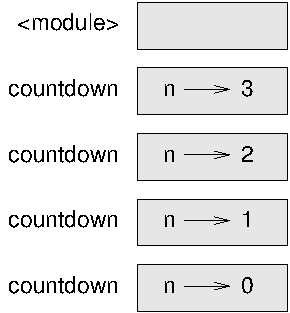
\includegraphics[scale=0.8]{figs/stack2.pdf}}
\caption{Stack diagram.}
\label{fig.stack2}
\end{figure}


As usual, the top of the stack is the frame for \verb"__main__".
It is empty because we did not create any variables in 
\verb"__main__" or pass any arguments to it.
\index{base case}
\index{recursion!base case}

通常,栈顶是\verb"__main__"的框架。
因为我们在\verb"__main__"中没有生成任何变量也没有传递任何实参给它,
所以它是空的。

The four {\tt countdown} frames have different values for the
parameter {\tt n}.  The bottom of the stack, where {\tt n=0}, is
called the {\bf base case}.  It does not make a recursive call, so
there are no more frames.

对于形参{\tt n},4个{\tt countdown}框架有不同的值。
栈底,其中{\tt n=0},被{\bf 基本条件(base case)}调用。
它不再进行递归调用了,所以没有更多的框架了。

\begin{exercise}
Draw a stack diagram for \verb"print_n" called with
\verb"s = 'Hello'" and {\tt n=2}.
\end{exercise}

\begin{exercise}
Write a function called \verb"do_n" that takes a function
object and a number, {\tt n}, as arguments, and that calls
the given function {\tt n} times.
\end{exercise}



\section{Infinite recursion 无限递归}
\index{infinite recursion}
\index{recursion!infinite}
\index{runtime error}
\index{error!runtime}
\index{traceback}

If a recursion never reaches a base case, it goes on making
recursive calls forever, and the program never terminates.  This is
known as {\bf infinite recursion}, and it is generally not
a good idea.  Here is a minimal program with an infinite recursion:

如果一个递归从不会到达基本条件,它永远进行递归调用,
并且程序从来不会终止。这被称作{\bf 无限递归(infinite recursion)},
通常这不是一个好主意。这是一个具有无限递归的微型程序:

\begin{verbatim}
def recurse():
    recurse()
\end{verbatim}
%
In most programming environments, a program with infinite recursion
does not really run forever.  Python reports an error
message when the maximum recursion depth is reached:
\index{exception!RuntimeError}
\index{RuntimeError}

在大多数编程环境里,一个具有无限递归的程序并非永远不会终止。
当达到最大递归深度时,Python报告一个错误信息:

\begin{verbatim}
  File "<stdin>", line 2, in recurse
  File "<stdin>", line 2, in recurse
  File "<stdin>", line 2, in recurse
                  .   
                  .
                  .
  File "<stdin>", line 2, in recurse
RuntimeError: Maximum recursion depth exceeded
\end{verbatim}
%
This traceback is a little bigger than the one we saw in the
previous chapter.  When the error occurs, there are 1000
{\tt recurse} frames on the stack!

此回溯比我们在前面章节看到的大一点。
当错误出现的时候,在栈上有1000个递归框架。

\section{Keyboard input 键盘输入}
\index{keyboard input}

The programs we have written so far are a bit rude in the sense that
they accept no input from the user.  They just do the same thing every
time.

到目前为止我们所写的程序都不接受来自用户的输入,从这个意义上讲有点儿粗鲁。
每次它们都只是做相同的事情。

Python 2 provides a built-in function called \verb"raw_input" that gets
input from the keyboard.  In Python 3, it is called
  {\tt input}.  When this function is called, the program stops and
waits for the user to type something.  When the user presses {\sf
  Return} or {\sf Enter}, the program resumes and \verb"raw_input"
returns what the user typed as a string.
\index{Python 3}
\index{raw\_input function}
\index{function!raw\_input}

Python 2提供了一个被称为\verb"raw_input"的内建函数,从键盘获得输入。
在Python 3中,它被称作{\tt input}。
当此函数被调用时,程序停下来并且等待用户键入一些东西。
当用户按回车时,程序恢复执行并且\verb"raw_input"作为字符串返回用户加入的内容。

\begin{verbatim}
>>> input = raw_input()
What are you waiting for?
>>> print input
What are you waiting for?
\end{verbatim}
%
Before getting input from the user, it is a good idea to print a
prompt telling the user what to input.  \verb"raw_input" can take a
prompt as an argument:
\index{prompt}

在从用户哪儿获得输入之前,打印一个提示告诉用户输入什么是个好办法。
\verb"raw_input"能接受一个提示作为实参。

\begin{verbatim}
>>> name = raw_input('What...is your name?\n')
What...is your name?
Arthur, King of the Britons!
>>> print name
Arthur, King of the Britons!
\end{verbatim}
%
The sequence \verb"\n" at the end of the prompt represents a {\bf newline},
which is a special character that causes a line break.
That's why the user's input appears below the prompt.
\index{newline}

提示最后的序列\verb"\n"表示一个{\bf 新行(newline)},
它是一个特别的字符,引起一个断行。
这也是为什么用户的输入出现在提示符的下面。

If you expect the user to type an integer, you can try to convert
the return value to {\tt int}:

如果你期望用户键入一个整数,那么你可以试着将返回值转化为{\tt int}:

\begin{verbatim}
>>> prompt = 'What...is the airspeed velocity of an unladen swallow?\n'
>>> speed = raw_input(prompt)
What...is the airspeed velocity of an unladen swallow?
17
>>> int(speed)
17
\end{verbatim}
%
But if the user types something other than a string of digits,
you get an error:

但是,如果用户键入非数字字符串的其它东西,你获得一个错误:

\begin{verbatim}
>>> speed = raw_input(prompt)
What...is the airspeed velocity of an unladen swallow?
What do you mean, an African or a European swallow?
>>> int(speed)
ValueError: invalid literal for int()
\end{verbatim}
%
We will see how to handle this kind of error later.
\index{ValueError}
\index{exception!ValueError}

我们后面将会看到如何处理这类错误。

\section{Debugging 调试}
\label{whitespace}
\index{debugging}
\index{traceback}

The traceback Python displays when an error occurs contains
a lot of information, but it can be overwhelming, especially
when there are many frames on the stack.  The most
useful parts are usually:

当一个错误发生时,Python显示的回溯包含许多信息,
但是它可能被淹没了,特别是在栈上有有许多框架时。
最有用的部分通常是:

\begin{itemize}

\item What kind of error it was, and

错误是哪类,以及

\item Where it occurred.

它发生在哪儿。

\end{itemize}

Syntax errors are usually easy to find, but there are a few
gotchas.  Whitespace errors can be tricky because spaces and
tabs are invisible and we are used to ignoring them.
\index{whitespace}

语法错误通常很容易被找到,但也有一些难度。
空白分隔符错误很棘手,因为空格和制表符是不可见的而且我们会忽略它们。

\begin{verbatim}
>>> x = 5
>>>  y = 6
  File "<stdin>", line 1
    y = 6
    ^
SyntaxError: invalid syntax
\end{verbatim}
%
In this example, the problem is that the second line is indented by
one space.  But the error message points to {\tt y}, which is
misleading.  In general, error messages indicate where the problem was
discovered, but the actual error might be earlier in the code,
sometimes on a previous line.
\index{error!runtime}
\index{runtime error}

在这个例子中,问题是第二行被一个空格缩进了。
但是错误信息指向{\tt y},这是个误导。
通常,错误信息指向被发现错误的地方,
但是真实的错误可能在代码中的更早前的地方,
有时在前一行。

The same is true of runtime errors.  

运行时错误也同样。

Suppose you are trying
to compute a signal-to-noise ratio in decibels.  The formula
is $SNR_{db} = 10 \log_{10} (P_{signal} / P_{noise})$.  In Python,
you might write something like this:

假设你正试图给计算机键入一个信噪比。
公式是$SNR_{db} = 10 \log_{10} (P_{signal} / P_{noise})$。
在Python中,你可能如此写:

\begin{verbatim}
import math
signal_power = 9
noise_power = 10
ratio = signal_power / noise_power
decibels = 10 * math.log10(ratio)
print decibels
\end{verbatim}
%
But when you run it in Python 2, you get an error message.
\index{exception!OverflowError}
\index{OverflowError}

但是,当你在Python 2中运行它的时候,
你获得一个错误信息。

\begin{verbatim}
Traceback (most recent call last):
  File "snr.py", line 5, in ?
    decibels = 10 * math.log10(ratio)
OverflowError: math range error
\end{verbatim}
%
The error message indicates line 5, but there is nothing
wrong with that line.  To find the real error, it might be
useful to print the value of {\tt ratio}, which turns out to
be 0.  The problem is in line 4, because dividing two integers
does floor division.  The solution is to represent signal power
and noise power with floating-point values.
\index{floor division}
\index{division!floor}

该错误信息指向第5行,但是那一行没什么错误。
为了找到真实的错误,打印{\tt ratio}也许会有用,它变成了0。
问题是在第4行,因为两个整数的除法是向下取整除。
解决办法是用浮点值表示信号功率和噪声功率。

In general, error messages tell you where the problem was discovered, 
but that is often not where it was caused.

通常,错误信息告诉你问题在哪儿发现的,但那经常并是非引起错误的地方。

In Python 3, this example does not cause an error; the division operator
performs floating-point division even with integer operands.

在Python 3中,此例不会引起一个错误。
即使是对整数运算数,除法运算符执行浮点除


\section{Glossary 术语表}

\begin{description}

\item[modulus operator(求余运算符):]  An operator, denoted with a percent sign
({\tt \%}), that works on integers and yields the remainder when one
number is divided by another.
\index{modulus operator}
\index{operator!modulus}

\item[boolean expression(布尔表达式):]  An expression whose value is either 
{\tt True} or {\tt False}.
\index{boolean expression}
\index{expression!boolean}

\item[relational operator(关系运算符):] One of the operators that compares
its operands: {\tt ==}, {\tt !=}, {\tt >}, {\tt <}, {\tt >=}, and {\tt <=}.

\item[logical operator:] One of the operators that combines boolean
expressions: {\tt and}, {\tt or}, and {\tt not}.

\item[conditional statement(条件语句):]  A statement that controls the flow of
execution depending on some condition.
\index{conditional statement}
\index{statement!conditional}

\item[condition(条件):] The boolean expression in a conditional statement
that determines which branch is executed.
\index{condition}

\item[compound statement(合成语句):]  A statement that consists of a header
and a body.  The header ends with a colon (:).  The body is indented
relative to the header.
\index{compound statement}

\item[branch(分支):] One of the alternative sequences of statements in
a conditional statement.
\index{branch}

\item[chained conditional(链式条件):]  A conditional statement with a series
of alternative branches.
\index{chained conditional}
\index{conditional!chained}

\item[nested conditional(嵌套条件):]  A conditional statement that appears
in one of the branches of another conditional statement.
\index{nested conditional}
\index{conditional!nested}

\item[recursion(递归):]  The process of calling the function that is
currently executing.
\index{recursion}

\item[base case(基本条件):]  A conditional branch in a
recursive function that does not make a recursive call.
\index{base case}

\item[infinite recursion(无限递归):]  A recursion that doesn't have a
base case, or never reaches it.  Eventually, an infinite recursion
causes a runtime error.
\index{infinite recursion}

\end{description}

\section{Exercises}

\begin{exercise}
\index{Fermat's Last Theorem}

Fermat's Last Theorem says that there are no integers
$a$, $b$, and $c$ such that

\[ a^n + b^n = c^n \]
%
for any values of $n$ greater than 2.

\begin{enumerate}

\item Write a function named \verb"check_fermat" that takes four
parameters---{\tt a}, {\tt b}, {\tt c} and {\tt n}---and
that checks to see if Fermat's theorem holds.  If
$n$ is greater than 2 and it turns out to be true that 

\[a^n + b^n = c^n \]
%
the program should print, ``Holy smokes, Fermat was wrong!''
Otherwise the program should print, ``No, that doesn't work.''

\item Write a function that prompts the user to input values
for {\tt a}, {\tt b}, {\tt c} and {\tt n}, converts them to
integers, and uses \verb"check_fermat" to check whether they
violate Fermat's theorem.

\end{enumerate}

\end{exercise}


\begin{exercise}
\index{triangle}

If you are given three sticks, you may or may not be able to arrange
them in a triangle.  For example, if one of the sticks is 12 inches
long and the other two are one inch long, it is clear that you will
not be able to get the short sticks to meet in the middle.  For any
three lengths, there is a simple test to see if it is possible to form
a triangle:

\begin{quotation}
If any of the three lengths is greater than the sum of the other
  two, then you cannot form a triangle.  Otherwise, you
  can.  (If the sum of two lengths equals the third, they form
    what is called a ``degenerate'' triangle.)
\end{quotation}

\begin{enumerate}

\item Write a function named \verb"is_triangle" that takes three
  integers as arguments, and that prints either ``Yes'' or ``No,'' depending
  on whether you can or cannot form a triangle from sticks with the
  given lengths.

\item Write a function that prompts the user to input three stick
  lengths, converts them to integers, and uses \verb"is_triangle" to
  check whether sticks with the given lengths can form a triangle.

\end{enumerate}

\end{exercise}

The following exercises use TurtleWorld from Chapter~\ref{turtlechap}:
\index{TurtleWorld}

\begin{exercise}

Read the following function and see if you can figure out
what it does.  Then run it (see the examples in Chapter~\ref{turtlechap}).

\begin{verbatim}
def draw(t, length, n):
    if n == 0:
        return
    angle = 50
    fd(t, length*n)
    lt(t, angle)
    draw(t, length, n-1)
    rt(t, 2*angle)
    draw(t, length, n-1)
    lt(t, angle)
    bk(t, length*n)
\end{verbatim}

\end{exercise}


\begin{figure}
\centerline
{
\includegraphics[scale=0.8]{figs/koch.pdf}}
\caption{A Koch curve.}
\label{fig.koch}
\end{figure}

\begin{exercise}
\index{Koch curve}

The Koch curve is a fractal that looks something like
Figure~\ref{fig.koch}.  To draw a Koch curve with length $x$, all you
have to do is

\begin{enumerate}

\item Draw a Koch curve with length $x/3$.

\item Turn left 60 degrees.

\item Draw a Koch curve with length $x/3$.

\item Turn right 120 degrees.

\item Draw a Koch curve with length $x/3$.

\item Turn left 60 degrees.

\item Draw a Koch curve with length $x/3$.

\end{enumerate}

The exception is if $x$ is less than 3: in that case,
you can just draw a straight line with length $x$.

\begin{enumerate}

\item Write a function called {\tt koch} that takes a turtle and
a length as parameters, and that uses the turtle to draw a Koch
curve with the given length.

\item Write a function called {\tt snowflake} that draws three
Koch curves to make the outline of a snowflake.

Solution: \url{http://thinkpython.com/code/koch.py}.

\item The Koch curve can be generalized in several ways.  See
\url{http://en.wikipedia.org/wiki/Koch_snowflake} for examples and
implement your favorite.

\end{enumerate}
\end{exercise}


\chapter{Fruitful functions 有返回值的函数}
\label{fruitchap}

\section{Return values 返回值}
\index{return value}

Some of the built-in functions we have used, such as the math
functions, produce results.  Calling the function generates a
value, which we usually assign to a variable or use as part of an
expression.

有一些我们用过的内建函数,例如数学函数,产生结果。
调用此函数产生一个值,通常我们将其赋给一个变量或者作为一个表达式的一部分使用。

\begin{verbatim}
e = math.exp(1.0)
height = radius * math.sin(radians)
\end{verbatim}
%
All of the functions we have written so far are void; they print
something or move turtles around, but their return value is {\tt
None}.

目前为止所有我们写的函数都是无返回值的,
它们打印一些东西或者移动海龟,但是它们的返回值是{\tt None}。

In this chapter, we are (finally) going to write fruitful functions.
The first example is {\tt area}, which returns the area of a circle
with the given radius:

在本章中,我们(最后)将写有返回值的函数。
第一个例子是{\tt area},给出半径,其返回一个圆的面积。

\begin{verbatim}
def area(radius):
    temp = math.pi * radius**2
    return temp
\end{verbatim}
%
We have seen the {\tt return} statement before, but in a fruitful
function the {\tt return} statement includes
an expression.  This statement means: ``Return immediately from
this function and use the following expression as a return value.''
The expression can be arbitrarily complicated, so we could
have written this function more concisely:
\index{return statement}
\index{statement!return}

之前我们已经见过{\tt return}语句了,但是在一个有返回值的函数中,
{\tt return}语句包含一个表达式。
这条语句意思是:``马上从该函数返回并使用下面的表达式作为返回值''。
此表达式可以是任意复杂的,因此我们可以将该函数写得更简洁些:

\begin{verbatim}
def area(radius):
    return math.pi * radius**2
\end{verbatim}
%
On the other hand, {\bf temporary variables} like {\tt temp} often make
debugging easier.
\index{temporary variable}
\index{variable!temporary}

另一方面,类似{\tt temp}的{\bf 临时变量(temporary variables)}经常会使调试更容易些。

Sometimes it is useful to have multiple return statements, one in each
branch of a conditional:

有时,有多个返回语句会很有用,在每个条件的分支内有一个。

\begin{verbatim}
def absolute_value(x):
    if x < 0:
        return -x
    else:
        return x
\end{verbatim}
%
Since these {\tt return} statements are in an alternative conditional,
only one will be executed.

既然这些{\tt return}语句在不同的条件内,只有一个会被执行。

As soon as a return statement executes, the function
terminates without executing any subsequent statements.
Code that appears after a {\tt return} statement, or any other place
the flow of execution can never reach, is called {\bf dead code}.
\index{dead code}

一旦一条返回语句执行,函数则终止,不再执行后续的语句。

In a fruitful function, it is a good idea to ensure
that every possible path through the program hits a
{\tt return} statement.  For example:

在一个有返回值的函数中,
保证通过程序的每个可能的路径都遇到一个{\tt return}语句是个好注意。
例如:

\begin{verbatim}
def absolute_value(x):
    if x < 0:
        return -x
    if x > 0:
        return x
\end{verbatim}
%
This function is incorrect because if {\tt x} happens to be 0,
neither condition is true, and the function ends without hitting a
{\tt return} statement.  If the flow of execution gets to the end
of a function, the return value is {\tt None}, which is not
the absolute value of 0.
\index{None special value}
\index{special value!None}

该函数是不正确的,因为如果{\tt x}恰好是0,
则没有条件为真,并且函数在没遇到任何{\tt return}语句条件下终止。
如果执行流到达函数的结尾,则返回值是{\tt None},
它不是0的绝对值。

\begin{verbatim}
>>> print absolute_value(0)
None
\end{verbatim}
%
By the way, Python provides a built-in function called 
{\tt abs} that computes absolute values.
\index{abs function}
\index{function!abs}

顺便说一下,Python提供一个被称为{\tt abs}的内建函数用来计算绝对值。

\begin{exercise}
\index{compare function}
\index{function!compare}

Write a {\tt compare} function
that returns {\tt 1} if {\tt x > y},
{\tt 0} if {\tt x == y}, and {\tt -1} if {\tt x < y}.
\end{exercise}


\section{Incremental development 增量式开发}
\label{incremental.development}
\index{development plan!incremental}

As you write larger functions, you might find yourself
spending more time debugging.

当你写较大的函数时,你可能发现你自己花了大量的时间用于调试。

To deal with increasingly complex programs,
you might want to try a process called
{\bf incremental development}.  The goal of incremental development
is to avoid long debugging sessions by adding and testing only
a small amount of code at a time.
\index{testing!incremental development}
\index{Pythagorean theorem}

为了对付越来越负责的程序,
你可能想试一种叫做{\bf 增量式开发(incremental development)}的过程。
增量式开发的目标是通过每次增加和测试一小部分代码,以避免调试长代码。

As an example, suppose you want to find the distance between two
points, given by the coordinates $(x_1, y_1)$ and $(x_2, y_2)$.
By the Pythagorean theorem, the distance is:

作为一个例子,假设给定两个点的坐标$(x_1, y_1)$和$(x_2, y_2)$,
你想计算两个点之间的距离。通过毕达哥拉斯定力,距离是:

\begin{displaymath}
\mathrm{distance} = \sqrt{(x_2 - x_1)^2 + (y_2 - y_1)^2}
\end{displaymath}
%
The first step is to consider what a {\tt distance} function should
look like in Python.  In other words, what are the inputs (parameters)
and what is the output (return value)?

第一步是考虑在Python中,一个{\tt distance}函数看起来会是什么样。
换句话说,输入(形参)和输出(返回值)是什么?

In this case, the inputs are two points, which you can represent
using four numbers.  The return value is the distance, which is
a floating-point value.

此例中,输入是可以用4个数表示的两个点。
返回值是距离,其是一个浮点数。

Already you can write an outline of the function:

因此,你可以写出此函数的轮廓:

\begin{verbatim}
def distance(x1, y1, x2, y2):
    return 0.0
\end{verbatim}
%
Obviously, this version doesn't compute distances; it always returns
zero.  But it is syntactically correct, and it runs, which means that
you can test it before you make it more complicated.

显然,此版本不能计算距离,它总是返回0。
但它是语法上正确的,并且它能运行,
也就是说在你将它变得更复杂之前,你能够测试它。

To test the new function, call it with sample arguments:

为了测试这个新函数,使用样例实参调用它:

\begin{verbatim}
>>> distance(1, 2, 4, 6)
0.0
\end{verbatim}
%
I chose these values so that the horizontal distance is 3 and the
vertical distance is 4; that way, the result is 5
(the hypotenuse of a 3-4-5 triangle). When testing a function, it is
useful to know the right answer.
\index{testing!knowing the answer}

我选择这些值以便水平距离是3,垂直距离是4。
这样结果是5(3-4-5三角形直角三角形的斜边)。
当测试一个函数时,知道正确的结果很有用。

At this point we have confirmed that the function is syntactically
correct, and we can start adding code to the body.
A reasonable next step is to find the differences
$x_2 - x_1$ and $y_2 - y_1$.  The next version stores those values in
temporary variables and prints them.

在这一点上,我们已经确定函数是语法正确的了,
我们可以在函数体中开始增加代码。
一个可行的下一步是找到$x_2 - x_1$和$y_2 - y_1$之间的不同。
下一个版本在临时变量中存储这些值并打印它们。

\begin{verbatim}
def distance(x1, y1, x2, y2):
    dx = x2 - x1
    dy = y2 - y1
    print 'dx is', dx
    print 'dy is', dy
    return 0.0
\end{verbatim}
%
If the function is working, it should display \verb"'dx is 3'" and {\tt
'dy is 4'}.  If so, we know that the function is getting the right
arguments and performing the first computation correctly.  If not,
there are only a few lines to check.

如果此函数好使,它应该显示\verb"'dx is 3'"以及{\tt 'dy is 4'}。
如果这样,我们知道此函数获得了正确的实参并且正确的执行第一步计算。
如果不是,只需检查很少的几行。

Next we compute the sum of squares of {\tt dx} and {\tt dy}:

下面我们计算{\tt dx}和{\tt dy}的平方和:

\begin{verbatim}
def distance(x1, y1, x2, y2):
    dx = x2 - x1
    dy = y2 - y1
    dsquared = dx**2 + dy**2
    print 'dsquared is: ', dsquared
    return 0.0
\end{verbatim}
%
Again, you would run the program at this stage and check the output
(which should be 25).
Finally, you can use {\tt math.sqrt} to compute and return the result:
\index{sqrt}
\index{function!sqrt}

再一次,你运行此程序并检查输出(它应该是25)。
最后,你可以使用{\tt math.sqrt}计算并返回结果:

\begin{verbatim}
def distance(x1, y1, x2, y2):
    dx = x2 - x1
    dy = y2 - y1
    dsquared = dx**2 + dy**2
    result = math.sqrt(dsquared)
    return result
\end{verbatim}
%
If that works correctly, you are done.  Otherwise, you might
want to print the value of {\tt result} before the return
statement.

如果其正确工作,你完成了。
否则,你可能想在返回语句之前打印返回值。

The final version of the function doesn't display anything when it
runs; it only returns a value.  The {\tt print} statements we wrote
are useful for debugging, but once you get the function working, you
should remove them.  Code like that is called {\bf scaffolding}
because it is helpful for building the program but is not part of the
final product.
\index{scaffolding}

当该函数的最终版本运行的时候,其不显示任何东西,它值返回一个值。
我们写的{\tt print}语句对于调试很有用,但是一旦你使得该寒素正确运行了,
你应该删除它们。类似的代码被称作{\bf 脚手架(scaffolding)},
因为它对建造程序很有用,但是不是最终产品的一部分。

When you start out, you should add only a line or two of code at a
time.  As you gain more experience, you might find yourself writing
and debugging bigger chunks.  Either way, incremental development
can save you a lot of debugging time.

当你刚开始的时候,你每次应该只增加一或两行代码。
随着你获得越来越多的经验,你可能发现你自己能写并调试更大的块了。
无论哪种方式,增量式开发能够节省你大量调试的时间。

The key aspects of the process are:

此过程的关键是:

\begin{enumerate}

\item Start with a working program and make small incremental changes. 
At any point, if there is an error, you should have a good idea
where it is.

从一个好使的程序开始并做小的增量式的修改。
如论何时,如果有一个错误,你应该知道它在哪儿。

\item Use temporary variables to hold intermediate values so you can
display and check them.

使用临时变量来存储中间值,因此你能显示并检查它们。

\item Once the program is working, you might want to remove some of
the scaffolding or consolidate multiple statements into compound
expressions, but only if it does not make the program difficult to
read.

一旦程序正常运行,你可能想删掉一些脚手架或者将多条语句组成复合表达式,
但是只有这不会使程序难读懂时。

\end{enumerate}

\begin{exercise}
\index{hypotenuse}

Use incremental development to write a function
called {\tt hypotenuse} that returns the length of the hypotenuse of a
right triangle given the lengths of the two legs as arguments.
Record each stage of the development process as you go.
\end{exercise}


\section{Composition 组合}
\index{composition}
\index{function composition}

As you should expect by now, you can call one function from
within another.  This ability is called {\bf composition}.

和你现在可能期望的一样,你可以从一个函数内部调用另一个函数。
这种能力被称作{\bf 组合(composition)}

As an example, we'll write a function that takes two points,
the center of the circle and a point on the perimeter, and computes
the area of the circle.

作为一个例子,我们将写一个接受两个点的函数,
圆心以及圆周上的一个点,然后计算此圆的面积。

Assume that the center point is stored in the variables {\tt xc} and
{\tt yc}, and the perimeter point is in {\tt xp} and {\tt yp}. The
first step is to find the radius of the circle, which is the distance
between the two points.  We just wrote a function, {\tt
distance}, that does that:

假设圆心点存储在变量{\tt xc}和{\tt yc}中,圆周点在{\tt xp}在{\tt yp}中。
第一步是计算圆的半径,其是两个点之间的距离。
我们刚写了一个函数{\tt distance}来做这个:

\begin{verbatim}
radius = distance(xc, yc, xp, yp)
\end{verbatim}
%
The next step is to find the area of a circle with that radius;
we just wrote that, too:

下一步是用那个半径计算一个圆的面积,我们也刚写过:

\begin{verbatim}
result = area(radius)
\end{verbatim}
%
Encapsulating these steps in a function, we get:
\index{encapsulation}

将这些步骤封装在一个函数中,我们获得:

\begin{verbatim}
def circle_area(xc, yc, xp, yp):
    radius = distance(xc, yc, xp, yp)
    result = area(radius)
    return result
\end{verbatim}
%
The temporary variables {\tt radius} and {\tt result} are useful for
development and debugging, but once the program is working, we can
make it more concise by composing the function calls:

临时变量{\tt radius}和{\tt result}对于开发和调试很有用,但是一旦改程序工作了,
我们可以通过组合函数调用,把它变得更简洁:

\begin{verbatim}
def circle_area(xc, yc, xp, yp):
    return area(distance(xc, yc, xp, yp))
\end{verbatim}
%

\section{Boolean functions 布尔函数}
\label{boolean}

Functions can return booleans, which is often convenient for hiding
complicated tests inside functions.  \index{boolean function}
For example:

函数能返回布尔值,将复杂的测试隐藏在函数中通常很方便。
例如:

\begin{verbatim}
def is_divisible(x, y):
    if x % y == 0:
        return True
    else:
        return False
\end{verbatim}
%
It is common to give boolean functions names that sound like yes/no
questions; \verb"is_divisible" returns either {\tt True} or {\tt False}
to indicate whether {\tt x} is divisible by {\tt y}.

通常给布尔函数一个听起来像是/否问题的函数名,
\verb"is_divisible"返回{\tt True}或{\tt False}来指示是否{\tt x}能被{\tt y}整除。

Here is an example:

这是一个例子:

\begin{verbatim}
>>>   is_divisible(6, 4)
False
>>>   is_divisible(6, 3)
True
\end{verbatim}
%
The result of the {\tt ==} operator is a boolean, so we can write the
function more concisely by returning it directly:

{\tt ==}运算符的结果是布尔值,
因此我们可以通过直接返回它更简洁的写出该函数:

\begin{verbatim}
def is_divisible(x, y):
    return x % y == 0
\end{verbatim}
%
Boolean functions are often used in conditional statements:
\index{conditional statement}
\index{statement!conditional}

布尔函数通常被用于条件语句中:

\begin{verbatim}
if is_divisible(x, y):
    print 'x is divisible by y'
\end{verbatim}
%
It might be tempting to write something like:

写一些类似的东西可能很诱人:

\begin{verbatim}
if is_divisible(x, y) == True:
    print 'x is divisible by y'
\end{verbatim}
%
But the extra comparison is unnecessary.

但是额外的比较是不必要的。

\begin{exercise}

Write a function \verb"is_between(x, y, z)" that
returns {\tt True} if $x \le y \le z$ or {\tt False} otherwise.

\end{exercise}


\section{More recursion 更多的递归}
\label{more.recursion}
\index{recursion}
\index{Turing complete language}
\index{language!Turing complete}
\index{Turing, Alan}
\index{Turing Thesis}

We have only covered a small subset of Python, but you might
be interested to know that this subset is a {\em complete}
programming language, which means that anything that can be
computed can be expressed in this language.  Any program ever written
could be rewritten using only the language features you have learned
so far (actually, you would need a few commands to control devices
like the keyboard, mouse, disks, etc., but that's all).

我们已经覆盖了Python的一个小的子集,
但是当你知道该子集是全部的编程语言时你可能很感兴趣,
这意味着任何能被计算的东西都能用该语言表达。
过去写的任何程序都能用你已经学过的语言特点表示
(事实上,你可能需要一些命令来控制如键盘、鼠标、磁盘等设备,但仅此而已)。

Proving that claim is a nontrivial exercise first accomplished by Alan
Turing, one of the first computer scientists (some would argue that he
was a mathematician, but a lot of early computer scientists started as
mathematicians).  Accordingly, it is known as the Turing Thesis.
For a more complete (and accurate) discussion of the Turing Thesis,
I recommend Michael Sipser's book {\em Introduction to the
Theory of Computation}.

证明这种说法是一个非凡的工作,首先由阿兰图灵完成,他是首批计算机科学家之一
(有些人认为他是一个数学家,但是很多早期的计算机科学家都开始是数学家)。
相应地,这被称作图灵理论。关于图灵理论更完整(和准确)的讨论,
我推荐Michael Sipser的书《Introduction to the Theory of Computation》。

To give you an idea of what you can do with the tools you have learned
so far, we'll evaluate a few recursively defined mathematical
functions.  A recursive definition is similar to a circular
definition, in the sense that the definition contains a reference to
the thing being defined.  A truly circular definition is not very
useful:

为了说明用目前学过的工具能做什么,我们将计算一些递归定义的数学函数。
递归定义类似循环定义,在这个意义上定义包含一个指向已经被定义的事物的引用。
一个真的循环定义不是非常有用:

\begin{description}

\item[vorpal:] An adjective used to describe something that is vorpal.
\index{vorpal}
\index{circular definition}
\index{definition!circular}

\item[漩涡:] 用一个形容词来描述漩涡状的东西。

\end{description}

If you saw that definition in the dictionary, you might be annoyed. On
the other hand, if you looked up the definition of the factorial
function, denoted with the symbol $!$, you might get something like
this:

如果你看到词典中的定义,你可能很恼火。
另一方面:如果你查找用$!$符号表示的阶乘函数的定义,
你可能获得如下的东西:
%
\begin{eqnarray*}
&&  0! = 1 \\
&&  n! = n (n-1)!
\end{eqnarray*}
%
This definition says that the factorial of 0 is 1, and the factorial
of any other value, $n$, is $n$ multiplied by the factorial of $n-1$.

此定义说0的阶乘是1,任何其它值$n$的阶乘是$n$乘以$n-1$的阶乘。

So $3!$ is 3 times $2!$, which is 2 times $1!$, which is 1 times
$0!$. Putting it all together, $3!$ equals 3 times 2 times 1 times 1,
which is 6.
\index{factorial function}
\index{function!factorial}
\index{recursive definition}

所以$3!$是3乘以$2!$,它又是2乘以$1!$,它又是1乘以$0!$。
将它放在一起,$3!$是3乘以2乘以1乘以1,是6。

If you can write a recursive definition of something, you can usually
write a Python program to evaluate it. The first step is to decide
what the parameters should be.  In this case it should be clear
that {\tt factorial} takes an integer:

如果你能写一些东西的递归定义,你通常可以写一个Python程序来计算它。
第一步是决定形参应该是什么。在此例中应该很清楚的是{\tt factorial}接受一个整数:

\begin{verbatim}
def factorial(n):
\end{verbatim}
%
If the argument happens to be 0, all we have to do is return 1:

如果实参恰好是0,所有我们需要做的是返回1:

\begin{verbatim}
def factorial(n):
    if n == 0:
        return 1
\end{verbatim}
%
Otherwise, and this is the interesting part, we have to make a
recursive call to find the factorial of $n-1$ and then multiply it by
$n$:

否则,这是一个很有趣的部分,我们必须进行递归调用来计算$n-1$的阶乘然后乘以$n$:

\begin{verbatim}
def factorial(n):
    if n == 0:
        return 1
    else:
        recurse = factorial(n-1)
        result = n * recurse
        return result
\end{verbatim}
%
The flow of execution for this program is similar to the flow of {\tt
countdown} in Section~\ref{recursion}.  If we call {\tt factorial}
with the value 3:

此程序的执行流程和\ref{recursion}节中的{\tt countdown}类似。
如果我们用值3调用{\tt factorial}:

Since 3 is not 0, we take the second branch and calculate the factorial
of {\tt n-1}...

既然3不是0,我们执行第二个分支并计算{\tt n-1}的阶乘…

\begin{quote}
Since 2 is not 0, we take the second branch and calculate the factorial of
{\tt n-1}...

既然2不是0,我们执行第二个分支并计算{\tt n-1}的阶乘…

  \begin{quote}
  Since 1 is not 0, we take the second branch and calculate the factorial
  of {\tt n-1}...

既然1不是0,我们执行第二个分支并计算{\tt n-1}的阶乘…

    \begin{quote}
    Since 0 {\em is} 0, we take the first branch and return 1
    without making any more recursive calls.
    
    既然0是0,我们执行第一个分支并返回1,不进行任何递归调用。
    \end{quote}


  The return value (1) is multiplied by $n$, which is 1, and the
  result is returned.
  
  返回值(1)被与$n$(其为1)相乘,并返回结果。
  \end{quote}


The return value (1) is multiplied by $n$, which is 2, and the
result is returned.

返回值(1)被与$n$(其为2)相乘,并返回结果。
\end{quote}


The return value (2) is multiplied by $n$, which is 3, and the result, 6,
becomes the return value of the function call that started the whole
process.

返回值(2)被与$n$(其为3)相乘,并返回结果6,成为整个过程开始调用的函数的返回值。
\index{stack diagram}

Figure~\ref{fig.stack3} shows what the stack diagram looks like for
this sequence of function calls.

图\ref{fig.stack3}显示了该函数调用序列的栈图看上去是什么样。

\begin{figure}
\centerline
{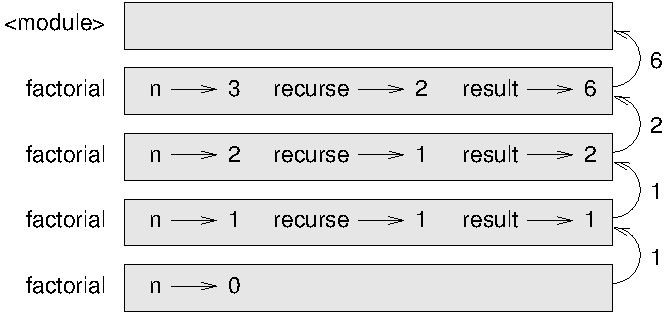
\includegraphics[scale=0.8]{figs/stack3.pdf}}
\caption{Stack diagram.}
\label{fig.stack3}
\end{figure}

The return values are shown being passed back up the stack.  In each
frame, the return value is the value of {\tt result}, which is the
product of {\tt n} and {\tt recurse}.
\index{function frame}
\index{frame}

返回值被显示为传回到栈顶。在每个框架中,返回值是{\tt result}的值,
其是{\tt n}和{\tt recurse}的乘积。

In the last frame, the local
variables {\tt recurse} and {\tt result} do not exist, because
the branch that creates them does not execute.

在最后一个框架中,局部变量{\tt recurse}和{\tt result}并不存在,
因为生成它们的分支并没有被执行。


\section{Leap of faith 信心的飞跃}
\index{recursion}
\index{leap of faith}

Following the flow of execution is one way to read programs, but
it can quickly become labyrinthine.  An
alternative is what I call the ``leap of faith.''  When you come to a
function call, instead of following the flow of execution, you {\em
assume} that the function works correctly and returns the right
result.

顺着执行流程读程序是一种方法,但是它可能很快变得错综复杂。
另一种是我称作``信心的飞跃''的方法。
当你遇到一个函数调用的时候,不是顺着执行流程,
而是假设该函数正确的工作并返回正确的结果。

In fact, you are already practicing this leap of faith when you use
built-in functions.  When you call {\tt math.cos} or {\tt math.exp},
you don't examine the bodies of those functions.  You just
assume that they work because the people who wrote the built-in
functions were good programmers.

事实上,当你使用内建函数的时候,你已经实践过这种方法了。
当你调用{\tt math.cos}或{\tt math.exp}时,你并没有检查那些函数的函数体。
你只是假设它们工作,因为写这些内建函数的人们都是好的程序员。

The same is true when you call one of your own functions.  For
example, in Section~\ref{boolean}, we wrote a function called 
\verb"is_divisible" that determines whether one number is divisible by
another.  Once we have convinced ourselves that this function is
correct---by examining the code and testing---we can use the function
without looking at the body again.
\index{testing!leap of faith}

当你调用一个你自己的函数时也是这样。
例如,在\ref{boolean}节中,我们写了一个称作\verb"is_divisible"的函数,
它决定是否一个数能被另一个整除。
一旦我们相信该函数是正确的---通过检查代码和测试---
我们就能能使用该函数,而不用再看函数体了。

The same is true of recursive programs.  When you get to the recursive
call, instead of following the flow of execution, you should assume
that the recursive call works (yields the correct result) and then ask
yourself, ``Assuming that I can find the factorial of $n-1$, can I
compute the factorial of $n$?''  In this case, it is clear that you
can, by multiplying by $n$.

递归程序也是这样。当你遇到递归调用时,
不用顺着执行流程,你应该假设次递归调用工作(产生正确的结果)
然后问你自己,``假设我能够获得$n-1$的阶乘,我能计算$n$的阶乘么?''
在此例中,很明显你能,通过乘以$n$。

Of course, it's a bit strange to assume that the function works
correctly when you haven't finished writing it, but that's why
it's called a leap of faith!

当然,当你没写完它的时候,假设函数正确工作有一点儿奇怪,
但这也是为什么这被称作信心的飞跃了!


\section{One more example 一个更多的例子}
\label{one.more.example}

\index{fibonacci function}
\index{function!fibonacci}
After {\tt factorial}, the most common example of a recursively
defined mathematical function is {\tt fibonacci}, which has the
following definition (see
  \url{http://en.wikipedia.org/wiki/Fibonacci_number}):
  
{\tt factorial}之后,最通常的一个被递归定义的数学函数是{\tt fibonacci},
其定义如下(见:\url{http://en.wikipedia.org/wiki/Fibonacci_number}):
%
\begin{eqnarray*}
&& \mathrm{fibonacci}(0) = 0 \\
&& \mathrm{fibonacci}(1) = 1 \\
&& \mathrm{fibonacci}(n) = \mathrm{fibonacci}(n-1) + \mathrm{fibonacci}(n-2)
\end{eqnarray*}
%
Translated into Python, it looks like this:

翻译成Python看起来是这样:

\begin{verbatim}
def fibonacci (n):
    if n == 0:
        return 0
    elif  n == 1:
        return 1
    else:
        return fibonacci(n-1) + fibonacci(n-2)
\end{verbatim}
%
If you try to follow the flow of execution here, even for fairly
small values of $n$, your head explodes.  But according to the
leap of faith, if you assume that the two recursive calls
work correctly, then it is clear that you get
the right result by adding them together.
\index{flow of execution}

这里,如果你试图跟随执行流程,即使对于相当小的$n$,
你的头也会爆炸。但是根据信心的飞跃,如果你假设这两个递归调用正确的工作,
那么很明显通过把它们加到一起,你获得了正确的结果。


\section{Checking types 检查类型}
\label{guardian}

What happens if we call {\tt factorial} and give it 1.5 as an argument?
\index{type checking}
\index{error checking}
\index{factorial function}
\index{RuntimeError}

如果我们将1.5作为实参调用{\tt factorial}会发生什么呢?

\begin{verbatim}
>>> factorial(1.5)
RuntimeError: Maximum recursion depth exceeded
\end{verbatim}
%
It looks like an infinite recursion.  But how can that be?  There is a
base case---when {\tt n == 0}.  But if {\tt n} is not an integer,
we can {\em miss} the base case and recurse forever.
\index{infinite recursion}
\index{recursion!infinite}

看上去像是一个无限循环。但那是如何发生的的?
有一个基本条件---当{\tt n == 0}时。
但是如果{\tt n}不是一个整数,我们会错过此基本条件并永远递归下去。

In the first recursive call, the value of {\tt n} is 0.5.
In the next, it is -0.5.  From there, it gets smaller
(more negative), but it will never be 0.

在第一个递归调用中,{\tt n}是0.5。下一次,它是-0.5。
从此,它变得越来越小(越来越负),但不会是0。

We have two choices.  We can try to generalize the {\tt factorial}
function to work with floating-point numbers, or we can make {\tt
  factorial} check the type of its argument.  The first option is
called the gamma function and it's a
little beyond the scope of this book.  So we'll go for the second.
\index{gamma function}

我们有两个选择。我们可以试着泛化{\tt factorial}函数使其能处理浮点数,
或者我们可以让{\tt factorial}检查它的实参的类型。
第一个选项被称作gamma函数,它有点儿超过本书的范围了。
所以我们将用第二种方法。

We can use the built-in function {\tt isinstance} to verify the type
of the argument.  While we're at it, we can also make sure the
argument is positive:
\index{isinstance function}
\index{function!isinstance}

我们可以使用内建函数{\tt isinstance}来验证实参的类型。
此时,我们也可以确保该实参是正数:

\begin{verbatim}
def factorial (n):
    if not isinstance(n, int):
        print 'Factorial is only defined for integers.'
        return None
    elif n < 0:
        print 'Factorial is not defined for negative integers.'
        return None
    elif n == 0:
        return 1
    else:
        return n * factorial(n-1)
\end{verbatim}
%
The first base case handles nonintegers; the
second catches negative integers.  In both cases, the program prints
an error message and returns {\tt None} to indicate that something
went wrong:

第一个基本条件处理非整数,第二个抓住负整数。
在这两个条件中,程序打印一个错误信息并返回{\tt None}以指明一些东西是错误的:

\begin{verbatim}
>>> factorial('fred')
Factorial is only defined for integers.
None
>>> factorial(-2)
Factorial is not defined for negative integers.
None
\end{verbatim}
% 
If we get past both checks, then we know that $n$ is positive or
zero, so we can prove that the recursion terminates.
\index{guardian pattern}
\index{pattern!guardian}

如果我们通过了这两个检查,那么我们知道$n$是一个正数或0,
因此我们可以保证递归终止。

This program demonstrates a pattern sometimes called a {\bf guardian}.
The first two conditionals act as guardians, protecting the code that
follows from values that might cause an error.  The guardians make it
possible to prove the correctness of the code.

此程序演示了一个模式,有时称作{\bf 监护人(guardian)}。
前两个条件扮演监护人的角色,避免下面的代码使用引起错误的值。
该监护人使得验证代码的正确性成为可能。

In Section~\ref{raise} we will see a more flexible alternative to printing
an error message: raising an exception.

在\ref{raise}节中,我们将看到更灵活的方法来打印错误信息:
抛出一个异常。

\section{Debugging 调试}
\label{factdebug}

Breaking a large program into smaller functions creates natural
checkpoints for debugging.  \index{debugging}
If a function is not working, there are
three possibilities to consider:

将一个大程序分解为较小的函数自然地为调试生成了检查点。
如果一个函数不工作,有三个可能需要考虑:

\begin{itemize}

\item There is something wrong with the arguments the function
is getting; a precondition is violated.

该函数获得的实参有些错误,违反先决条件。

\item There is something wrong with the function; a postcondition
is violated.

该函数有些错误,违反后置条件。

\item There is something wrong with the return value or the
way it is being used.

返回值或者它的使用方法有错误。

\end{itemize}

To rule out the first possibility, you can add a {\tt print} statement
at the beginning of the function and display the values of the
parameters (and maybe their types).  Or you can write code
that checks the preconditions explicitly.
\index{precondition}
\index{postcondition}

为了排除第一种可能,你可以在函数的开始增加一条{\tt print}语句
来显示形参的值(也可能是它们的类型)。
或者你可以写代码来显示地检查先决条件。

If the parameters look good, add a {\tt print} statement before each
{\tt return} statement that displays the return value.  If
possible, check the result by hand.  Consider calling the
function with values that make it easy to check the result
(as in Section~\ref{incremental.development}).

如果形参看起来很好,在每个{\tt return}语句之前增加一条{\tt print}语句,
来显示返回值。如果可能,手工检查结果。
考虑用一些容易检查的值来调用该函数(类似在\ref{incremental.development}节中)。

If the function seems to be working, look at the function call
to make sure the return value is being used correctly (or used
at all!).
\index{flow of execution}

如果该函数看起来工作,则看函数调用确保返回值被正确的使用(或者被用了!)

Adding print statements at the beginning and end of a function
can help make the flow of execution more visible.
For example, here is a version of {\tt factorial} with
print statements:

在一个函数的开始和结束增加打印语句可以帮助执行流程更明显。
例如,这是{\tt factorial}的具有打印语句的版本:

\begin{verbatim}
def factorial(n):
    space = ' ' * (4 * n)
    print space, 'factorial', n
    if n == 0:
        print space, 'returning 1'
        return 1
    else:
        recurse = factorial(n-1)
        result = n * recurse
        print space, 'returning', result
        return result
\end{verbatim}
%
{\tt space} is a string of space characters that controls the
indentation of the output.  Here is the result of {\tt factorial(5)} :

{\tt space}是一个空格字符的字符串,用来控制输出的缩进。
这是{\tt factorial(5)}的结果:

\begin{verbatim}
                     factorial 5
                 factorial 4
             factorial 3
         factorial 2
     factorial 1
 factorial 0
 returning 1
     returning 1
         returning 2
             returning 6
                 returning 24
                     returning 120
\end{verbatim}
%
If you are confused about the flow of execution, this kind of
output can be helpful.  It takes some time to develop effective
scaffolding, but a little bit of scaffolding can save a lot of debugging.

如果你对执行流程感到困惑,这种输出可能有用。
开发有效的脚手架会花些时间,但是一点点的脚手架能够节省调试的时间。

\section{Glossary 术语表}

\begin{description}

\item[temporary variable(临时变量):]  A variable used to store an intermediate value in
a complex calculation.
\index{temporary variable}
\index{variable!temporary}

\item[dead code(死代码):]  Part of a program that can never be executed, often because
it appears after a {\tt return} statement.
\index{dead code}

\item[{\tt None} (空):]  A special value returned by functions that
have no return statement or a return statement without an argument.
\index{None special value}
\index{special value!None}

\item[incremental development(增量式开发):]  A program development plan intended to
avoid debugging by adding and testing only
a small amount of code at a time.
\index{incremental development}

\item[scaffolding(脚手架):]  Code that is used during program development but is
not part of the final version.
\index{scaffolding}

\item[guardian(监护人):]  A programming pattern that uses a conditional
statement to check for and handle circumstances that
might cause an error.
\index{guardian pattern}
\index{pattern!guardian}

\end{description}


\section{Exercises}

\begin{exercise}

Draw a stack diagram for the following program.  What does the program print?
Solution: \url{http://thinkpython.com/code/stack_diagram.py}.
\index{stack diagram}

\begin{verbatim}
def b(z):
    prod = a(z, z)
    print z, prod
    return prod

def a(x, y):
    x = x + 1
    return x * y

def c(x, y, z):
    total = x + y + z
    square = b(total)**2
    return square

x = 1
y = x + 1
print c(x, y+3, x+y)
\end{verbatim}

\end{exercise}


\begin{exercise}
\label{ackermann}

The Ackermann function, $A(m, n)$, is defined:

\begin{eqnarray*}
A(m, n) = \begin{cases} 
              n+1 & \mbox{if } m = 0 \\ 
        A(m-1, 1) & \mbox{if } m > 0 \mbox{ and } n = 0 \\ 
A(m-1, A(m, n-1)) & \mbox{if } m > 0 \mbox{ and } n > 0.
\end{cases} 
\end{eqnarray*}
%
See \url{http://en.wikipedia.org/wiki/Ackermann_function}.
Write a function named {\tt ack} that evaluates Ackermann's function.
Use your function to evaluate {\tt ack(3, 4)}, which should be 125.
What happens for larger values of {\tt m} and {\tt n}?
Solution: \url{http://thinkpython.com/code/ackermann.py}.
\index{Ackermann function}
\index{function!ack}

\end{exercise}


\begin{exercise}
\label{palindrome}

A palindrome is a word that is spelled the same backward and
forward, like ``noon'' and ``redivider''.  Recursively, a word
is a palindrome if the first and last letters are the same
and the middle is a palindrome.
\index{palindrome}

The following are functions that take a string argument and
return the first, last, and middle letters:

\begin{verbatim}
def first(word):
    return word[0]

def last(word):
    return word[-1]

def middle(word):
    return word[1:-1]
\end{verbatim}
%
We'll see how they work in Chapter~\ref{strings}.

\begin{enumerate}

\item Type these functions into a file named {\tt palindrome.py}
and test them out.  What happens if you call {\tt middle} with
a string with two letters?  One letter?  What about the empty
string, which is written \verb"''" and contains no letters?

\item Write a function called \verb"is_palindrome" that takes
a string argument and returns {\tt True} if it is a palindrome
and {\tt False} otherwise.  Remember that you can use the
built-in function {\tt len} to check the length of a string.

\end{enumerate}

Solution: \url{http://thinkpython.com/code/palindrome_soln.py}.

\end{exercise}

\begin{exercise}

A number, $a$, is a power of $b$ if it is divisible by $b$
and $a/b$ is a power of $b$.  Write a function called
\verb"is_power" that takes parameters {\tt a} and {\tt b}
and returns {\tt True} if {\tt a} is a power of {\tt b}.
Note: you will have to think about the base case.

\end{exercise}


\begin{exercise}
\index{greatest common divisor (GCD)}
\index{GCD (greatest common divisor)}

The greatest common divisor (GCD) of $a$ and $b$ is the largest number
that divides both of them with no remainder.  

One way to find the GCD of two numbers is Euclid's algorithm,
which is based on the observation that if $r$ is the remainder
when $a$ is divided by $b$, then $gcd(a, b) = gcd(b, r)$.
As a base case, we can use $gcd(a, 0) = a$.
\index{Euclid's algorithm}
\index{algorithm!Euclid}

Write a function called
\verb"gcd" that takes parameters {\tt a} and {\tt b}
and returns their greatest common divisor.  If you need
help, see \url{http://en.wikipedia.org/wiki/Euclidean_algorithm}.

Credit: This exercise is based on an example from Abelson and
Sussman's {\em Structure and Interpretation of Computer Programs}.

\end{exercise}


\chapter{Iteration 迭代}

\section{Multiple assignment 多次赋值}
\index{assignment}
\index{statement!assignment}
\index{multiple assignment}

As you may have discovered, it is legal to
make more than one assignment to the same variable.  A
new assignment makes an existing variable refer to a new
value (and stop referring to the old value).

如你可能已经发现的,对同一变量进行多次赋值是合法的。
一个新的赋值使一个已有变量指向一个新的值(并停止指向旧的值)。

\begin{verbatim}
bruce = 5
print bruce,
bruce = 7
print bruce
\end{verbatim}
%
The output of this program is {\tt 5 7}, because the first time
{\tt bruce} is printed, its value is 5, and the second time, its
value is 7.  The
comma at the end of the first {\tt print} statement suppresses
the newline, which is why both outputs
appear on the same line.
\index{newline}

程序的输出是{\tt 5 7},因为{\tt bruce}第一次被打印时,它的值是5,
第二次值是7。第一条{\tt print}语句结尾的逗号禁止产生新行,
这也是为什么两个输出出现在同一行上。

Figure~\ref{fig.assign2} shows what {\bf multiple assignment} looks
like in a state diagram. 
\index{state diagram} 
\index{diagram!state}

图\ref{fig.assign2}显示在一个栈图中,{\bf 多次赋值(multiple assignment)}
看起来是什么样子。

With multiple assignment it is especially important to distinguish
between an assignment operation and a statement of equality.  Because
Python uses the equal sign ({\tt =}) for assignment, it is tempting to
interpret a statement like {\tt a = b} as a statement of equality. It
is not!
\index{equality and assignment}

有了多次赋值,区分赋值运算和相等语句就特别重要。
因为Python使用等号({\tt =})表示赋值,
容易将类似{\tt a = b}的语句理解成一个相等语句,但它不是!

First, equality is a symmetric relation and assignment is not.  For
example, in mathematics, if $a=7$ then $7=a$.  But in Python, the
statement {\tt a = 7} is legal and {\tt 7 = a} is not.

首先,相等是一个对称关系但赋值不是。
例如,在数学中,如果$a=7$,那么$7=a$。
但是在Python中,{\tt a = 7}语句是合法的,但{\tt 7 = a}不合法。 

Furthermore, in mathematics, a statement of equality is either true or
false, for all time.  If $a=b$ now, then $a$ will always equal $b$.
In Python, an assignment statement can make two variables equal, but
they don't have to stay that way:

更进一步,在数学中,一个相等语句总是或者为真或者为假。
如果现在$a=b$,那么$a$总是等于$b$。
在Python中,一条赋值语句可以使两个变量相等,但是它们不必总保持那样:

\begin{verbatim}
a = 5
b = a    # a and b are now equal
a = 3    # a and b are no longer equal
\end{verbatim}
%
The third line changes the value of {\tt a} but does not change the
value of {\tt b}, so they are no longer equal. 

第三行改变了{\tt a}的值,但是不改变{\tt b}的值,因此它们不再相等。

Although multiple assignment is frequently helpful, you should use it
with caution.  If the values of variables change frequently, it can
make the code difficult to read and debug.

虽然多次赋值通常很有用,但是你应该小心使用它。
如果变量的值经常改变,可能使代码很难读和调试。

\begin{figure}
\centerline
{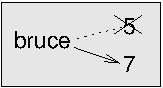
\includegraphics[scale=0.8]{figs/assign2.pdf}}
\caption{State diagram.}
\label{fig.assign2}
\end{figure}



\section{Updating variables 更新变量}
\label{update}

\index{update}
\index{variable!updating}

One of the most common forms of multiple assignment is an {\bf update},
where the new value of the variable depends on the old.

多次赋值的最常见形式之一是{\bf 更新(update)},
变量的新值依赖于旧值。

\begin{verbatim}
x = x+1
\end{verbatim}
%
This means ``get the current value of {\tt x}, add one, and then
update {\tt x} with the new value.''

这个意思是``获得{\tt x}的当前值,加1,然后用新值更新{\tt x}''。

If you try to update a variable that doesn't exist, you get an
error, because Python evaluates the right side before it assigns
a value to {\tt x}:

如果你试图更新一个不存在的变量,那么你会得到一个错误,
因为Python在给{\tt x}赋值之前,先计算右边的值。

\begin{verbatim}
>>> x = x+1
NameError: name 'x' is not defined
\end{verbatim}
%
Before you can update a variable, you have to {\bf initialize}
it, usually with a simple assignment:
\index{initialization (before update)}

在你可以更新一个变量之前,你必须{\bf 初始化(initialize)}它,
通常使用一个简单的赋值:

\begin{verbatim}
>>> x = 0
>>> x = x+1
\end{verbatim}
%
Updating a variable by adding 1 is called an {\bf increment};
subtracting 1 is called a {\bf decrement}.
\index{increment}
\index{decrement}


通过加1更新一个变量被称作{\bf 递增(increment)},
减1被称作{\bf 递减(decrement)}。



\section{The {\tt while} statement {\tt while}语句}
\index{statement!while}
\index{while loop}
\index{loop!while}
\index{iteration}

Computers are often used to automate repetitive tasks.  Repeating
identical or similar tasks without making errors is something that
computers do well and people do poorly.

计算机经常被用于自动重复的任务。
无误地重复相同或者相似的任务是计算能做得很好,而人做得不好的事情。

We have seen two programs, {\tt countdown} and \verb"print_n", that
use recursion to perform repetition, which is also called {\bf
iteration}.  Because iteration is so common, Python provides several
language features to make it easier.  One is the {\tt for} statement
we saw in Section~\ref{repetition}.  We'll get back to that later.

我们已经看过两个程序,{\tt countdown}和\verb"print_n",它们使用递归来执行重复,
这也被称作{\bf 迭代(iteration)}。因为迭代是如此常见,
以至于Python提供了几个语言特性来使它变得容易。
一个是我们在\ref{repetition}节中看到的{\tt for}语句。
我们后面会回到它。

Another is the {\tt while} statement.  Here is a version of {\tt
countdown} that uses a {\tt while} statement:

另一个是{\tt while}语句。这是使用{\tt while}语句的{\tt countdown}版本:

\begin{verbatim}
def countdown(n):
    while n > 0:
        print n
        n = n-1
    print 'Blastoff!'
\end{verbatim}
%
You can almost read the {\tt while} statement as if it were English.
It means, ``While {\tt n} is greater than 0,
display the value of {\tt n} and then reduce the value of
{\tt n} by 1.  When you get to 0, display the word {\tt Blastoff!}''
\index{flow of execution}

你几乎可以作为英语来读{\tt while}语句。
它的意思是,``当{\tt n}大于0时,显示{\tt n}的值,然后将{\tt n}的值减1。
当到达0的时候,显示单词{\tt Blastoff!}''。

More formally, here is the flow of execution for a {\tt while} statement:

更正式地,这是{\tt while}语句执行的流程:

\begin{enumerate}

\item Evaluate the condition, yielding {\tt True} or {\tt False}.

求条件的值,产生{\tt True}或者{\tt False}。

\item If the condition is false, exit the {\tt while} statement
and continue execution at the next statement.

如果条件为假,则退出{\tt while}语句并继续执行下一条语句。

\item If the condition is true, execute the
body and then go back to step 1.

如条件为真,则执行循环体然后回到步骤1。

\end{enumerate}

This type of flow is called a {\bf loop} because the third step
loops back around to the top.  
\index{condition}
\index{loop}
\index{body}

这类流程被称作{\bf 循环(loop)},因为第3步循环回顶部。

The body of the loop should change the value of one or more variables
so that eventually the condition becomes false and the loop
terminates.  Otherwise the loop will repeat forever, which is called
an {\bf infinite loop}.  An endless source of amusement for computer
scientists is the observation that the directions on shampoo,
``Lather, rinse, repeat,'' are an infinite loop.
\index{infinite loop}
\index{loop!infinite}

循环体应该改变一个或多个变量的值,以便最终条件变为假然后循环终止。
否则,循环永远重复下去,这被称作{\bf 无限循环(infinite loop)}。
对于计算机科学家一个消遣的无尽来源是观察香波的说明书,
``打泡沫,漂洗,重复'',就是无限循环。

In the case of {\tt countdown}, we can prove that the loop
terminates because we know that the value of {\tt n} is finite, and we
can see that the value of {\tt n} gets smaller each time through the
loop, so eventually we have to get to 0.  In other
cases, it is not so easy to tell:

在{\tt countdown}的例子中,我们可以证明循环能终止,
因为我们知道{\tt n}的值是有限的,
并且我们可以看到通过循环,{\tt n}的值每次都变小,
所以最终我们一定获得0。
在另一个例子中,就不这么简单了:

\begin{verbatim}
def sequence(n):
    while n != 1:
        print n,
        if n%2 == 0:        # n is even
            n = n/2
        else:               # n is odd
            n = n*3+1
\end{verbatim}
%
The condition for this loop is {\tt n != 1}, so the loop will continue
until {\tt n} is {\tt 1}, which makes the condition false.

该循环的条件是{\tt n != 1},所以循环将继续直到{\tt n}是{\tt 1},
这使得条件为假。

Each time through the loop, the program outputs the value of {\tt n}
and then checks whether it is even or odd.  If it is even, {\tt n} is 
divided by 2.  If it is odd, the value of {\tt n} is replaced with
{\tt n*3+1}. For example, if the argument passed
to {\tt sequence} is 3, the resulting sequence is 3, 10, 5, 16, 8, 4, 2, 1.

每次通过循环,程序输出{\tt n}的值,然后检查它是偶数还是奇数。
如果是偶数,{\tt n}被2除。如果是奇数,{\tt n}的值用{\tt n*3+1}代替。
例如,如果船体给{\tt sequence}的实参是3,
结果序列是3, 10, 5, 16, 8, 4, 2, 1。

Since {\tt n} sometimes increases and sometimes decreases, there is no
obvious proof that {\tt n} will ever reach 1, or that the program
terminates.  For some particular values of {\tt n}, we can prove
termination.  For example, if the starting value is a power of two,
then the value of {\tt n} will be even each time through the loop
until it reaches 1. The previous example ends with such a sequence,
starting with 16.
\index{Collatz conjecture}

既然{\tt n}有时增大,有时减小,所以没有明显的证明{\tt n}最终会到达1,
或者程序终止。对于一些特殊的{\tt n}值,我们能够证明终止。
例如,如果起始值是2的幂指数,那么通过循环,{\tt n}的值每次都是偶数直到它到达1.
前面的例子以16开始的这样的序列终止。

The hard question is whether we can prove that this program terminates
for {\em all positive values} of {\tt n}.  So far, no one has
been able to prove it {\em or} disprove it!  (See
  \url{http://en.wikipedia.org/wiki/Collatz_conjecture}.)
  
难题是是否我们能够证明该程序对于所有正数{\tt n}都会终止。
目前为止,没有人能证明它或者否定它!
(见:\url{http://en.wikipedia.org/wiki/Collatz_conjecture})。

\begin{exercise}

Rewrite the function \verb"print_n" from
Section~\ref{recursion} using iteration instead of recursion.

\end{exercise}


\section{{\tt break}}
\index{break statement}
\index{statement!break}

Sometimes you don't know it's time to end a loop until you get half
way through the body.  In that case you can use the {\tt break}
statement to jump out of the loop.

有时你到循环的一半才知道该结束循环了。
在此情况下,你可以使用{\tt break}语句跳出循环。

For example, suppose you want to take input from the user until they
type {\tt done}.  You could write:

例如,假设你想接受来自用户的输入直到他们键入{\tt done}。
你可以写成:

\begin{verbatim}
while True:
    line = raw_input('> ')
    if line == 'done':
        break
    print line

print 'Done!'
\end{verbatim}
%
The loop condition is {\tt True}, which is always true, so the
loop runs until it hits the break statement.

该循环条件是{\tt True},它总是真的,所以直到遇到{\tt break}语句,
循环将一直运行下去。

Each time through, it prompts the user with an angle bracket.
If the user types {\tt done}, the {\tt break} statement exits
the loop.  Otherwise the program echoes whatever the user types
and goes back to the top of the loop.  Here's a sample run:

每次循环,它用一个三角括号提示用户。
如果用户键入{\tt done},{\tt break}语句退出循环。
否则程序回应用户键入的任何东西并且回到循环的顶部。
这是一个运行样例:

\begin{verbatim}
> not done
not done
> done
Done!
\end{verbatim}
%
This way of writing {\tt while} loops is common because you
can check the condition anywhere in the loop (not just at the
top) and you can express the stop condition affirmatively
(``stop when this happens'') rather than negatively (``keep going
until that happens.'').

这种写{\tt while}循环的方法很常见,因为你可以在循环中任何位置检查条件
(不是仅在顶部)并且你可以积极地表达停止条件(``当此发生时停止''),
而不是消极地(``继续运行直到其发生'')。


\section{Square roots 平方根}
\label{squareroot}
\index{square root}

Loops are often used in programs that compute
numerical results by starting with an approximate answer and
iteratively improving it.
\index{Newton's method}

循环经常被用于计算数值结果的程序中,其开始于一个估计答案并迭代地改进它。

For example, one way of computing square roots is Newton's method.
Suppose that you want to know the square root of $a$.  If you start
with almost any estimate, $x$, you can compute a better
estimate with the following formula:

例如,一种计算平方根的方法是牛顿法。假设你想知道$a$的平方根。
如果你用任意一个估计值$x$开始,你可以用下面的公式计算一个更好的估计值:

\[ y = \frac{x + a/x}{2} \]
%
For example, if $a$ is 4 and $x$ is 3:

例如,如果$a$是4,$x$是3:

\begin{verbatim}
>>> a = 4.0
>>> x = 3.0
>>> y = (x + a/x) / 2
>>> print y
2.16666666667
\end{verbatim}
%
Which is closer to the correct answer ($\sqrt{4} = 2$).  If we
repeat the process with the new estimate, it gets even closer:

这和正确答案($\sqrt{4} = 2$)更接近了。
如果我们用这个新的估计重复这个过程,它甚至更进了:

\begin{verbatim}
>>> x = y
>>> y = (x + a/x) / 2
>>> print y
2.00641025641
\end{verbatim}
%
After a few more updates, the estimate is almost exact:
\index{update}

更多次的更新后,估计几乎是精确的:

\begin{verbatim}
>>> x = y
>>> y = (x + a/x) / 2
>>> print y
2.00001024003
>>> x = y
>>> y = (x + a/x) / 2
>>> print y
2.00000000003
\end{verbatim}
%
In general we don't know ahead of time how many steps it takes
to get to the right answer, but we know when we get there
because the estimate
stops changing:

一般来讲,我们事先不知道获得正确的答案需要多少步,
但是我们知道什么时候获得正确答案,因为估计值不再变化了:

\begin{verbatim}
>>> x = y
>>> y = (x + a/x) / 2
>>> print y
2.0
>>> x = y
>>> y = (x + a/x) / 2
>>> print y
2.0
\end{verbatim}
%
When {\tt y == x}, we can stop.  Here is a loop that starts
with an initial estimate, {\tt x}, and improves it until it
stops changing:

当{\tt y == x}时,我们可以停止。
下面是以一个初始估计{\tt x}开始的循环,然后改进它直到它停止改变

\begin{verbatim}
while True:
    print x
    y = (x + a/x) / 2
    if y == x:
        break
    x = y
\end{verbatim}
%
For most values of {\tt a} this works fine, but in general it is
dangerous to test {\tt float} equality.
Floating-point values are only approximately right:
most rational numbers, like $1/3$, and irrational numbers, like
$\sqrt{2}$, can't be represented exactly with a {\tt float}.
\index{floating-point}
\index{epsilon}

对于大多数{\tt a}其工作的很好,但是一般来讲测试{\tt float}相等很危险。
浮点数值只是估计正确的:大多数有理数,像$1/3$,以及无理数,
像$\sqrt{2}$不能用{\tt float}精确地表示。

Rather than checking whether {\tt x} and {\tt y} are exactly equal, it
is safer to use the built-in function {\tt abs} to compute the
absolute value, or magnitude, of the difference between them:

与其检查{\tt x}和{\tt y}是否精确地相等,
不如使用内建函数{\tt abs}来计算它们之间不同的绝对或者数量级更安全。

\begin{verbatim}
    if abs(y-x) < epsilon:
        break
\end{verbatim}
%
Where \verb"epsilon" has a value like {\tt 0.0000001} that
determines how close is close enough.

其中\verb"epsilon"的值类似{\tt 0.0000001},其决定多近是足够近了。

\begin{exercise}

Encapsulate this loop in a function called \verb"square_root"
that takes {\tt a} as a parameter, chooses a reasonable
value of {\tt x}, and returns an estimate of the square root
of {\tt a}.
\index{encapsulation}

\end{exercise}


\section{Algorithms 算法}
\index{algorithm}

Newton's method is an example of an {\bf algorithm}: it is a
mechanical process for solving a category of problems (in this
case, computing square roots).

牛顿法是一个{\bf 算法(algorithm)}的例子:
它是解决一类问题的机械化的过程(此例中是计算平方根)。

It is not easy to define an algorithm.  It might help to start
with something that is not an algorithm.  When you learned
to multiply single-digit numbers, you probably memorized the
multiplication table.  In effect, you memorized 100 specific solutions.
That kind of knowledge is not algorithmic.

定义算法并不容易。从一些不是算法的东西开始可能有帮助。
当你学习一位数相乘的时候,你可能记住乘法表。
实际上,你记下100个特定的答案。这类知识不是算法。

But if you were ``lazy,'' you probably cheated by learning a few
tricks.  For example, to find the product of $n$ and 9, you can
write $n-1$ as the first digit and $10-n$ as the second
digit.  This trick is a general solution for multiplying any
single-digit number by 9.  That's an algorithm!
\index{addition with carrying}
\index{carrying, addition with}
\index{subtraction!with borrowing}
\index{borrowing, subtraction with}

但是如果你``很懒'',你可能通过学习一些技巧来欺骗。
例如,为了计算$n$和9的乘积,你可以写下$n-1$作为第一位,
$10-n$作为第二位。这种技巧是任意位数字和9相乘的一般解决方案。
这是一个算法!

Similarly, the techniques you learned for addition with carrying,
subtraction with borrowing, and long division are all algorithms.  One
of the characteristics of algorithms is that they do not require any
intelligence to carry out.  They are mechanical processes in which
each step follows from the last according to a simple set of rules.

类似的,你学过的进位加法、借位减法以及长除技术都是算法。
算法的特点之一是它们不需要任何智慧来执行。
它们是机械的过程,每一步根据简单的规则集,跟着上一步执行。

In my opinion, it is embarrassing that humans spend so much time in
school learning to execute algorithms that, quite literally, require
no intelligence.

在我看来,人们在学校里花费如此大量的时间学习执行直白的,
不需要智力的算法真是很尴尬

On the other hand, the process of designing algorithms is interesting,
intellectually challenging, and a central part of what we call
programming.

另一方面,设计算法的过程是很有趣的,
充满智力的挑战并且是编程的核心部分。

Some of the things that people do naturally, without difficulty or
conscious thought, are the hardest to express algorithmically.
Understanding natural language is a good example.  We all do it, but
so far no one has been able to explain {\em how} we do it, at least
not in the form of an algorithm.

一些人们做得很自然、没什么难度或者有意识的思考的事情是最难用算法表示的。
理解自然语言是一个很好的例子。
我们都能做它,但是目前为止,没有人能解释我们是如何做的,
至少不能以算法的形式解释。


\section{Debugging 调试}

As you start writing bigger programs, you might find yourself
spending more time debugging.  More code means more chances to
make an error and more place for bugs to hide.
\index{debugging!by bisection}
\index{bisection, debugging by}

当你开始写较大的程序的时候,你可能发现你自己花了太多的时间在调试上。
更多的代码意味着更多的犯错机会以及更多隐藏错误的地方。

One way to cut your debugging time is ``debugging by bisection.''
For example, if there are 100 lines in your program and you
check them one at a time, it would take 100 steps.

一种减少调试时间的方法是``对分调试''。
例如,如果你的程序有100行,你每次检查一行,这将花费100步。

Instead, try to break the problem in half.  Look at the middle
of the program, or near it, for an intermediate value you
can check.  Add a {\tt print} statement (or something else
that has a verifiable effect) and run the program.

相反,试着将问题对半分。在程序的中间部分或则附近看一下你可以检查的中间值。
增加一条{\tt print}语句(或则其它有验证功能的东西)并运行程序。

If the mid-point check is incorrect, there must be a problem in the
first half of the program.  If it is correct, the problem is
in the second half.

如果中间检查点不正确,则前半部分必然有一个问题。
如果正确,则问题在后半部分。

Every time you perform a check like this, you halve the number of
lines you have to search.  After six steps (which is fewer than 100),
you would be down to one or two lines of code, at least in theory.

每次你执行类似的检查,你将你需要搜索的行数分了一半。
经过6步(少于100),至少在理论上你将下到一两行代码。

In practice it is not always clear what
the ``middle of the program'' is and not always possible to
check it.  It doesn't make sense to count lines and find the
exact midpoint.  Instead, think about places
in the program where there might be errors and places where it
is easy to put a check.  Then choose a spot where you
think the chances are about the same that the bug is before
or after the check.

在实践中,``程序的中间部分''是什么通常不是很清楚,
并且检查它也不总是可能的。数行数并找到精确的中间点也没什么意义。
相反,要考虑程序中可能犯错的地方以及容易设置检查点的地方。
然后选择一个你认为错误会在其之前或之后的检查点。

\section{Glossary 术语表}

\begin{description}

\item[multiple assignment(多次赋值):] Making more than one assignment to the same
variable during the execution of a program.
\index{multiple assignment}
\index{assignment!multiple}

\item[update(更新):] An assignment where the new value of the variable
depends on the old.
\index{update}

\item[initialization(初始化):] An assignment that gives an initial value to
a variable that will be updated.
\index{initialization!variable}

\item[increment(递增):] An update that increases the value of a variable
(often by one).
\index{increment}

\item[decrement(递减):] An update that decreases the value of a variable.
\index{decrement}

\item[iteration(迭代):] Repeated execution of a set of statements using
either a recursive function call or a loop.
\index{iteration}

\item[infinite loop(无限循环):] A loop in which the terminating condition is
never satisfied.
\index{infinite loop}

\end{description}


\section{Exercises}

\begin{exercise}
\index{algorithm!square root}

To test the square root algorithm in this chapter, you could compare
it with {\tt math.sqrt}.  Write a function named \verb"test_square_root"
that prints a table like this:

\begin{verbatim}
1.0 1.0           1.0           0.0
2.0 1.41421356237 1.41421356237 2.22044604925e-16
3.0 1.73205080757 1.73205080757 0.0
4.0 2.0           2.0           0.0
5.0 2.2360679775  2.2360679775  0.0
6.0 2.44948974278 2.44948974278 0.0
7.0 2.64575131106 2.64575131106 0.0
8.0 2.82842712475 2.82842712475 4.4408920985e-16
9.0 3.0           3.0           0.0

\end{verbatim}
%
The first column is a number, $a$; the second column is
the square root of $a$ computed with the function from
Section~\ref{squareroot}; the third column is the square root computed
by {\tt math.sqrt}; the fourth column is the absolute value
of the difference between the two estimates.
\end{exercise}


\begin{exercise}
\index{eval function}
\index{function!eval}

The built-in function {\tt eval} takes a string and evaluates
it using the Python interpreter.  For example:

\begin{verbatim}
>>> eval('1 + 2 * 3')
7
>>> import math
>>> eval('math.sqrt(5)')
2.2360679774997898
>>> eval('type(math.pi)')
<type 'float'>
\end{verbatim}
%
Write a function called \verb"eval_loop" that iteratively
prompts the user, takes the resulting input and evaluates
it using {\tt eval}, and prints the result.

It should continue until the user enters \verb"'done'", and then
return the value of the last expression it evaluated.

\end{exercise}


\begin{exercise}
\index{Ramanujan, Srinivasa}

The mathematician Srinivasa Ramanujan found an
infinite series
that can be used to generate a numerical
approximation of $\pi$:
\index{pi}

\[ \frac{1}{\pi} = \frac{2\sqrt{2}}{9801} 
\sum^\infty_{k=0} \frac{(4k)!(1103+26390k)}{(k!)^4 396^{4k}} \]

Write a function called \verb"estimate_pi" that uses this formula
to compute and return an estimate of $\pi$.  It should use a {\tt while}
loop to compute terms of the summation until the last term is
smaller than {\tt 1e-15} (which is Python notation for $10^{-15}$).
You can check the result by comparing it to {\tt math.pi}.

Solution: \url{http://thinkpython.com/code/pi.py}.

\end{exercise}


\chapter{Strings 字符串}
\label{strings}


\section{A string is a sequence 字符串是一个序列}

\index{sequence}
\index{character}
\index{bracket operator}
\index{operator!bracket}
A string is a {\bf sequence} of characters.  
You can access the characters one at a time with the
bracket operator:

一个字符串是一个字符的{\bf 序列(sequence)}。
你可以用括号运算符一次访问一个字符:

\begin{verbatim}
>>> fruit = 'banana'
>>> letter = fruit[1]
\end{verbatim}
%
The second statement selects character number 1 from {\tt
fruit} and assigns it to {\tt letter}.  
\index{index}

第2条语句从{\tt fruit}中选择编号为1的字符并将它赋给{\tt letter}。

The expression in brackets is called an {\bf index}.  
The index indicates which character in the sequence you
want (hence the name).

括号中的表达式被称作{\bf 索引(index)}。
索引指出在序列中你想要哪个字符(因此而得名)。

But you might not get what you expect:

但是你可能不会获得你期望的东西:

\begin{verbatim}
>>> print letter
a
\end{verbatim}
%
For most people, the first letter of \verb"'banana'" is {\tt b}, not
{\tt a}.  But for computer scientists, the index is an offset from the
beginning of the string, and the offset of the first letter is zero.

对于大多数人,\verb"'banana'"的第一个字母是{\tt b}而不是{\tt a}。
但是对于计算机科学家,索引是从字符串开始的偏移量,
并且第一个字母的偏移量是0。

\begin{verbatim}
>>> letter = fruit[0]
>>> print letter
b
\end{verbatim}
%
So {\tt b} is the 0th letter (``zero-eth'') of \verb"'banana'", {\tt a}
is the 1th letter (``one-eth''), and {\tt n} is the 2th (``two-eth'')
letter.
\index{index!starting at zero}
\index{zero, index starting at}

所以{\tt b}是\verb"'banana'"的第0个字母(``zero-eth''),
{\tt a}是第1个字母(``one-eth''),{\tt n}是第2个字母(``two-eth'')。

You can use any expression, including variables and operators, as an
index, but the value of the index has to be an integer.  Otherwise you
get:
\index{index}
\index{exception!TypeError}
\index{TypeError}

你可以使用任何表达式,包括变量名和运算符,都可以做为索引,
但是索引的值必须是整数。否则你获得:

\begin{verbatim}
>>> letter = fruit[1.5]
TypeError: string indices must be integers
\end{verbatim}
%

\section{{\tt len}}
\index{len function}
\index{function!len}

{\tt len} is a built-in function that returns the number of characters
in a string:

{\tt len}是一个内建函数,其返回字符串中的字符数:

\begin{verbatim}
>>> fruit = 'banana'
>>> len(fruit)
6
\end{verbatim}
%
To get the last letter of a string, you might be tempted to try something
like this:
\index{exception!IndexError}
\index{IndexError}

为了获得一个字符串的最后一个字符,你可能想尝试像这样:

\begin{verbatim}
>>> length = len(fruit)
>>> last = fruit[length]
IndexError: string index out of range
\end{verbatim}
%
The reason for the {\tt IndexError} is that there is no letter in {\tt
'banana'} with the index 6.  Since we started counting at zero, the
six letters are numbered 0 to 5.  To get the last character, you have
to subtract 1 from {\tt length}:

{\tt IndexError}的理由是在{\tt 'banana'}中没有索引为6的字母。
既然我们从0开始数数,6个字母的编号是0到5。
为了获得最后一个字符,你必须从{\tt length}中减1。

\begin{verbatim}
>>> last = fruit[length-1]
>>> print last
a
\end{verbatim}
%
Alternatively, you can use negative indices, which count backward from
the end of the string.  The expression {\tt fruit[-1]} yields the last
letter, {\tt fruit[-2]} yields the second to last, and so on.
\index{index!negative}
\index{negative index}

另一种作法是你可以使用负索引,其从字符串的结尾往后数。
表达式{\tt fruit[-1]}产生最后一个字母,{\tt fruit[-2]}产生倒数第二个字母,等等。


\section{Traversal with a {\tt for} loop 使用{\tt for}循环遍历}
\label{for}
\index{traversal}
\index{loop!traversal}
\index{for loop}
\index{loop!for}
\index{statement!for}
\index{traversal}

A lot of computations involve processing a string one character at a
time.  Often they start at the beginning, select each character in
turn, do something to it, and continue until the end.  This pattern of
processing is called a {\bf traversal}.  One way to write a traversal
is with a {\tt while} loop:

许多计算每次处理一个字符串的字符。
它们经常从头开始,依次选择每个字符,对其做一些工作,然后继续直到结束。
词处理模式被称作{\bf 遍历(traversal)}。
一种写遍历的方法是用{\tt while}循环:

\begin{verbatim}
index = 0
while index < len(fruit):
    letter = fruit[index]
    print letter
    index = index + 1
\end{verbatim}
%
This loop traverses the string and displays each letter on a line by
itself.  The loop condition is {\tt index < len(fruit)}, so
when {\tt index} is equal to the length of the string, the
condition is false, and the body of the loop is not executed.  The
last character accessed is the one with the index {\tt len(fruit)-1},
which is the last character in the string.

该循环遍历字符串并显示在每行显示一个字符串。
该循环的条件是{\tt index < len(fruit)},所以当{\tt index}和字符串的长度相等时,
条件为假,并且循环体不被执行。
被访问的最后一个字符的索引为{\tt len(fruit)-1},
这是字符串的最后一个字符。

\begin{exercise}

Write a function that takes a string as an argument
and displays the letters backward, one per line.

\end{exercise}

Another way to write a traversal is with a {\tt for} loop:

另一种写遍历的方法是用{\tt for}循环:

\begin{verbatim}
for char in fruit:
    print char
\end{verbatim}
%
Each time through the loop, the next character in the string is assigned
to the variable {\tt char}.  The loop continues until no characters are
left.
\index{concatenation}
\index{abecedarian}
\index{McCloskey, Robert}

每次通过循环,字符串中的下一个字符被赋给变量{\tt char}。
循环继续,直到没有剩余的字符串了。

The following example shows how to use concatenation (string addition)
and a {\tt for} loop to generate an abecedarian series (that is, in
alphabetical order).  In Robert McCloskey's book {\em Make
Way for Ducklings}, the names of the ducklings are Jack, Kack, Lack,
Mack, Nack, Ouack, Pack, and Quack.  This loop outputs these names in
order:

下面的例子显示如何使用叠加(字符串加)和{\tt for}循环生成一个字母系列(以字母序)。
在Robert McCloskey的书《Make Way for Ducklings》中,
小鸭子的名字是Jack, Kack, Lack, Mack, Nack, Ouack, Pack, and Quack。
此循环按顺序输出这些名字:

\begin{verbatim}
prefixes = 'JKLMNOPQ'
suffix = 'ack'

for letter in prefixes:
    print letter + suffix
\end{verbatim}
%
The output is:

输出是:

\begin{verbatim}
Jack
Kack
Lack
Mack
Nack
Oack
Pack
Qack
\end{verbatim}
%
Of course, that's not quite right because ``Ouack'' and
``Quack'' are misspelled.

当然,这不是非常正确,因为``Ouack''和``Quack''被错误拼写了。

\begin{exercise}

Modify the program to fix this error.

\end{exercise}



\section{String slices 字符串切片}
\label{slice}
\index{slice operator}
\index{operator!slice}
\index{index!slice}
\index{string!slice}
\index{slice!string}

A segment of a string is called a {\bf slice}.  Selecting a slice is
similar to selecting a character:

一段字符串被称作{\bf 切片(slice)}。
选择一个切片类似于选择一个字符:

\begin{verbatim}
>>> s = 'Monty Python'
>>> print s[0:5]
Monty
>>> print s[6:12]
Python
\end{verbatim}
%
The operator {\tt [n:m]} returns the part of the string from the 
``n-eth'' character to the ``m-eth'' character, including the first but
excluding the last.  This behavior is counterintuitive, but it might
help to imagine the indices pointing {\em between} the
characters, as in Figure~\ref{fig.banana}.

{\tt [n:m]}操作符返回从第n个字符到第m个字符的部分字符串,
包括第一个,但是不包括最后一个。
这个行为违反直觉,但是它可能会帮助想象指向这两个字符之间的索引,
如图\ref{fig.banana}。

\begin{figure}
\centerline
{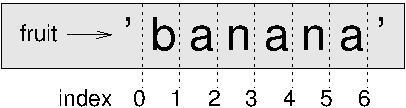
\includegraphics[scale=0.8]{figs/banana.pdf}}
\caption{Slice indices.}
\label{fig.banana}
\end{figure}


If you omit the first index (before the colon), the slice starts at
the beginning of the string.  If you omit the second index, the slice
goes to the end of the string:

如果你省略第一个索引(冒号前面的),切片起始于字符串开始。
如果你省略第二个索引,切片一直到字符串结尾:

\begin{verbatim}
>>> fruit = 'banana'
>>> fruit[:3]
'ban'
>>> fruit[3:]
'ana'
\end{verbatim}
%
If the first index is greater than or equal to the second the result
is an {\bf empty string}, represented by two quotation marks:
\index{quotation mark}

如果第一个索引大于或等于第二个,结果是{\bf 空字符串(empty string)},
表示为两个引号:

\begin{verbatim}
>>> fruit = 'banana'
>>> fruit[3:3]
''
\end{verbatim}
%
An empty string contains no characters and has length 0, but other
than that, it is the same as any other string.

一个空字符串不包括字符而且长度为0,但除此之外,
它和其它任何字符串一样。

\begin{exercise}

Given that {\tt fruit} is a string, what does
{\tt fruit[:]} mean?
\index{copy!slice}
\index{slice!copy}

\end{exercise}


\section{Strings are immutable 字符串是不可变的}
\index{mutability}
\index{immutability}
\index{string!immutable}

It is tempting to use the {\tt []} operator on the left side of an
assignment, with the intention of changing a character in a string.
For example:
\index{TypeError}
\index{exception!TypeError}

在一个赋值的左边使用{\tt []}很有诱惑力,意图是改变字符串的一个字符。
例如:

\begin{verbatim}
>>> greeting = 'Hello, world!'
>>> greeting[0] = 'J'
TypeError: object does not support item assignment
\end{verbatim}
%
The ``object'' in this case is the string and the ``item'' is
the character you tried to assign.  For now, an {\bf object} is
the same thing as a value, but we will refine that definition
later.  An {\bf item} is one of the values in a sequence.
\index{object}
\index{item assignment}
\index{assignment!item}
\index{immutability}

此例中的``object(对象)''是该字符串,``item(项)''是你要赋值的字符。
到目前,一个{\bf 对象(object)}和值是同一样的东西,
但是我们后面将改善此定义。一个{\bf 项(item)}是序列中的一个值。

The reason for the error is that
strings are {\bf immutable}, which means you can't change an
existing string.  The best you can do is create a new string
that is a variation on the original:

此错误的原因是字符串是{\bf 不可变的(immutable)},
这意味着你不能改变一个已存在的字符串。
最好是生成一个新的字符串,它是原字符串的一个变种:

\begin{verbatim}
>>> greeting = 'Hello, world!'
>>> new_greeting = 'J' + greeting[1:]
>>> print new_greeting
Jello, world!
\end{verbatim}
%
This example concatenates a new first letter onto
a slice of {\tt greeting}.  It has no effect on
the original string.
\index{concatenation}

此例连接一个新的第一个字母到{\tt greeting}的一个切片上。
它不影响原字符串。

\section{Searching 搜索}
\label{find}

What does the following function do?
\index{find function}
\index{function!find}

下面的函数做什么?

\begin{verbatim}
def find(word, letter):
    index = 0
    while index < len(word):
        if word[index] == letter:
            return index
        index = index + 1
    return -1
\end{verbatim}
%
In a sense, {\tt find} is the opposite of the {\tt []} operator.
Instead of taking an index and extracting the corresponding character,
it takes a character and finds the index where that character
appears.  If the character is not found, the function returns {\tt
-1}.

在某种意义上,{\tt find}和{\tt []}运算符相反。
不是接受一个索引并抽取相应的字符,
它接受一个字符并找到该字符出现的位置的索引。
如果没有找到该字符,函数返回{\tt -1}。

This is the first example we have seen of a {\tt return} statement
inside a loop.  If {\tt word[index] == letter}, the function breaks
out of the loop and returns immediately.

这是我们已经见过的第一个{\tt return}语句在循环内部的例子。
如果{\tt word[index] == letter},函数停止循环并马上返回。

If the character doesn't appear in the string, the program
exits the loop normally and  returns {\tt -1}.

如果字符没出现在字符串中,那么程序正常退出循环并返回{\tt -1}。

This pattern of computation---traversing a sequence and returning
when we find what we are looking for---is called a {\bf search}.
\index{traversal}
\index{search pattern}
\index{pattern!search}

这种计算的模式---遍历一个序列并在我们找到我们正在找的东西时返回---
被称作{\bf 搜索(search)}。

\begin{exercise}

Modify {\tt find} so that it has a
third parameter, the index in {\tt word} where it should start
looking.

\end{exercise}


\section{Looping and counting 循环和计数}
\label{counter}
\index{counter}
\index{counting and looping}
\index{looping and counting}
\index{looping!with strings}

The following program counts the number of times the letter {\tt a}
appears in a string:

下面的程序计算字母{\tt a}在字符串中出现的次数:

\begin{verbatim}
word = 'banana'
count = 0
for letter in word:
    if letter == 'a':
        count = count + 1
print count
\end{verbatim}
%
This program demonstrates another pattern of computation called a {\bf
counter}.  The variable {\tt count} is initialized to 0 and then
incremented each time an {\tt a} is found.
When the loop exits, {\tt count}
contains the result---the total number of {\tt a}'s.

此程序演示另一种被称作{\bf 计数器(counter)}的计算模式。
变量{\tt count}初始化为0然后每次出现{\tt a}时递增。
当循环结束时,{\tt count}包含结果---{\tt a}的总数。

\begin{exercise}
\index{encapsulation}

Encapsulate this code in a function named {\tt
count}, and generalize it so that it accepts the string and the
letter as arguments.
\end{exercise}

\begin{exercise}

Rewrite this function so that instead of
traversing the string, it uses the three-parameter version of {\tt
find} from the previous section.

\end{exercise}


\section{String methods 字符串方法}

A {\bf method} is similar to a function---it takes arguments and
returns a value---but the syntax is different.  For example, the
method {\tt upper} takes a string and returns a new string with
all uppercase letters:
\index{method}
\index{string!method}

{\bf 方法(method)}和函数类似---接受实参并返回一个值---但是语法不同。
例如,{\bf upper}方法接受一个字符串并返回一个新的都是大写字母的字符串:

Instead of the function syntax {\tt upper(word)}, it uses
the method syntax {\tt word.upper()}.
\index{dot notation}

不是用函数的语法{\tt upper(word)},而是用方法的语法{\tt word.upper()}。

\begin{verbatim}
>>> word = 'banana'
>>> new_word = word.upper()
>>> print new_word
BANANA
\end{verbatim}
%
This form of dot notation specifies the name of the method, {\tt
upper}, and the name of the string to apply the method to, {\tt
word}.  The empty parentheses indicate that this method takes no
argument.
\index{parentheses!empty}

点号的形式指出方法的名字,{\tt upper},以及应用该方法的字符串的名字,{\tt word}。
空括号指出该方法不接受实参。

A method call is called an {\bf invocation}; in this case, we would
say that we are invoking {\tt upper} on the {\tt word}.
\index{invocation}

方法的调用被称作{\bf 调用(invocation)},在此例中,
我们说我们整在{\tt word}上调用{\tt upper}。

As it turns out, there is a string method named {\tt find} that
is remarkably similar to the function we wrote:

事实上,有一个被称为{\tt find}的字符串方法,
其和我们写的函数异常相似:

\begin{verbatim}
>>> word = 'banana'
>>> index = word.find('a')
>>> print index
1
\end{verbatim}
%
In this example, we invoke {\tt find} on {\tt word} and pass
the letter we are looking for as a parameter.

此例中,我们在{\tt word}上调用{\tt find}并将我们要找的字母作为实参。

Actually, the {\tt find} method is more general than our function;
it can find substrings, not just characters:

事实上,{\tt find}方法比我们的函数更通用,它可以找到子串而不仅仅是字符:

\begin{verbatim}
>>> word.find('na')
2
\end{verbatim}
%
It can take as a second argument the index where it should start:
\index{optional argument}
\index{argument!optional}

它可以接受从何处开始的索引作为第二个实参:

\begin{verbatim}
>>> word.find('na', 3)
4
\end{verbatim}
%
And as a third argument the index where it should stop:

在哪个索引结束作为第三个实参。

\begin{verbatim}
>>> name = 'bob'
>>> name.find('b', 1, 2)
-1
\end{verbatim}
%
This search fails because {\tt b} does not
appear in the index range from {\tt 1} to {\tt 2} (not including {\tt
2}).

此搜索失败是因为{\tt b}没有出现在从{\tt 1}到{\tt 2}的索引之间
(不包括{\tt 2})。


\begin{exercise}
\index{count method}
\index{method!count}

There is a string method called {\tt count} that is similar
to the function in the previous exercise.  Read the documentation
of this method
and write an invocation that counts the number of {\tt a}s
in \verb"'banana'".
\end{exercise}


\begin{exercise}
\index{string method}
\index{method!string}

Read the documentation of the string methods at
\url{docs.python.org/lib/string-methods.html}.  You
might want to experiment with some of them to make sure
you understand how they work.  {\tt strip} and
{\tt replace} are particularly useful.

The documentation uses a syntax that might be confusing.
For example, in \verb"find(sub[, start[, end]])", the brackets
indicate optional arguments.  So {\tt sub} is required, but
{\tt start} is optional, and if you include {\tt start},
then {\tt end} is optional.
\end{exercise}


\section{The {\tt in} operator {\tt in}运算符}
\label{inboth}
\index{in operator}
\index{operator!in}
\index{boolean operator}
\index{operator!boolean}

The word {\tt in} is a boolean operator that takes two strings and
returns {\tt True} if the first appears as a substring in the second:

单词{\tt in}是一个布尔运算符,其接受两个字符串,
如果第一个作为子串出现在第二个中则返回{\tt True}:

\begin{verbatim}
>>> 'a' in 'banana'
True
>>> 'seed' in 'banana'
False
\end{verbatim}
%
For example, the following function prints all the
letters from {\tt word1} that also appear in {\tt word2}:

例如,下面的函数打印即出现在{\tt word1}中也出现在{\tt word2}中的字母:

\begin{verbatim}
def in_both(word1, word2):
    for letter in word1:
        if letter in word2:
            print letter
\end{verbatim}
%
With well-chosen variable names,
Python sometimes reads like English.  You could read
this loop, ``for (each) letter in (the first) word, if (the) letter 
(appears) in (the second) word, print (the) letter.''

使用精心挑选的变量名,Python有时候读起来像是英语。
你可以读此循环,``对于(每个)在(第一个)单词中的字母,
如果(该)字母 (出现)在(第二个)单词中,打印(该)字母''。

Here's what you get if you compare apples and oranges:

如果你比较apples和oranges,这是你获得的东西:

\begin{verbatim}
>>> in_both('apples', 'oranges')
a
e
s
\end{verbatim}
%

\section{String comparison 字符串比较}
\index{string!comparison}
\index{comparison!string}

The relational operators work on strings.  To see if two strings are equal:

关系运算符在字符串上也工作。为了看两个字符串是否相等:

\begin{verbatim}
if word == 'banana':
    print 'All right, bananas.'
\end{verbatim}
%
Other relational operations are useful for putting words in alphabetical
order:

其它的关系运算符对于按字母序放置单词也很有用:

\begin{verbatim}
if word < 'banana':
    print 'Your word,' + word + ', comes before banana.'
elif word > 'banana':
    print 'Your word,' + word + ', comes after banana.'
else:
    print 'All right, bananas.'
\end{verbatim}
%
Python does not handle uppercase and lowercase letters the same way
that people do.  All the uppercase letters come before all the
lowercase letters, so:

Python用和人不同的方式处理大写和小写字母。
所有的大写字母出现在所有小写字母之前,所以:

\begin{verbatim}
Your word, Pineapple, comes before banana.
\end{verbatim}
%
A common way to address this problem is to convert strings to a
standard format, such as all lowercase, before performing the
comparison.  Keep that in mind in case you have to defend yourself
against a man armed with a Pineapple.

解决此问题的通常的方式是在执行比较之前,
将字符串转化为标准格式,例如都是小写字母。
一旦你必须保卫自己免受一名手持菠萝的男子的袭击,记住这一点。

\section{Debugging 调试}
\index{debugging}
\index{traversal}

When you use indices to traverse the values in a sequence,
it is tricky to get the beginning and end of the traversal
right.  Here is a function that is supposed to compare two
words and return {\tt True} if one of the words is the reverse
of the other, but it contains two errors:

当你使用索引在一个序列中遍历值的时候,
正确的获得遍历的开始和结束是一个技巧。
这是一个函数,其被假设用来比较两个单词,
如果一个单词是另一个的倒序,则返回真,
但是它包含两个错误:

\begin{verbatim}
def is_reverse(word1, word2):
    if len(word1) != len(word2):
        return False
    
    i = 0
    j = len(word2)

    while j > 0:
        if word1[i] != word2[j]:
            return False
        i = i+1
        j = j-1

    return True
\end{verbatim}
%
The first {\tt if} statement checks whether the words are the
same length.  If not, we can return {\tt False} immediately
and then, for the rest of the function, we can assume that the words
are the same length.  This is an example of the guardian pattern
in Section~\ref{guardian}.
\index{guardian pattern}
\index{pattern!guardian}
\index{index}

第一条{\tt if}语句检查两个单词是否等长。
如果不是,我们可以马上返回假,然后对于函数其余的部分,
我们可以假设单词是等长的。
这是\ref{guardian}节中的监护人模式的一个例子。

{\tt i} and {\tt j} are indices: {\tt i} traverses {\tt word1}
forward while {\tt j} traverses {\tt word2} backward.  If we find
two letters that don't match, we can return {\tt False} immediately.
If we get through the whole loop and all the letters match, we
return {\tt True}.

{\tt i}和{\tt j}是索引:{\tt i}向前遍历{\tt word1},{\tt j}向后遍历{\tt word2}。
如果我们找到两个不匹配的字母,我们可以立即返回假。
如果我们通过整个循环并且所有字母都匹配,我们返回真。

If we test this function with the words ``pots'' and ``stop'', we
expect the return value {\tt True}, but we get an IndexError:
\index{IndexError}
\index{exception!IndexError}

如果我们用单词``pots''和``stop''测试该函数,我们期望返回真,
但是我们得到一个IndexError。

\begin{verbatim}
>>> is_reverse('pots', 'stop')
...
  File "reverse.py", line 15, in is_reverse
    if word1[i] != word2[j]:
IndexError: string index out of range
\end{verbatim}
%
For debugging this kind of error, my first move is to
print the values of the indices immediately before the line
where the error appears.

为了调试该类错误,我的第一步是在错误出现的行之前,马上打印索引的值。

\begin{verbatim}
    while j > 0:
        print i, j        # print here
        
        if word1[i] != word2[j]:
            return False
        i = i+1
        j = j-1
\end{verbatim}
%
Now when I run the program again, I get more information:

现在,当我再次运行该程序时,我获得更多的信息:

\begin{verbatim}
>>> is_reverse('pots', 'stop')
0 4
...
IndexError: string index out of range
\end{verbatim}
%
The first time through the loop, the value of {\tt j} is 4,
which is out of range for the string \verb"'pots'".
The index of the last character is 3, so the
initial value for {\tt j} should be {\tt len(word2)-1}.
\index{semantic error}
\index{error!semantic}

第一次通过循环,{\tt j}的值是4,其超出字符串\verb"'pots'"的范围了。
最后一个字符的索引是3,所以{\tt j}的初始值应该是{\tt len(word2)-1}。

If I fix that error and run the program again, I get:

如果我修正了这个错误并重新运行程序,我获得:

\begin{verbatim}
>>> is_reverse('pots', 'stop')
0 3
1 2
2 1
True
\end{verbatim}
%
This time we get the right answer, but it looks like the loop only ran
three times, which is suspicious.  To get a better idea of what is
happening, it is useful to draw a state diagram.  During the first
iteration, the frame for \verb"is_reverse" is shows in Figure~\ref{fig.state4}.
\index{state diagram}
\index{diagram!state}

这次,我获得正确的答案,但是看起来循环只运行了三次,这很奇怪。
为了更好的理解发生了什么,画出栈图会很有用。
在第一次循环期间,\verb"is_reverse"的框架显示在图\ref{fig.state4}中。

\begin{figure}
\centerline
{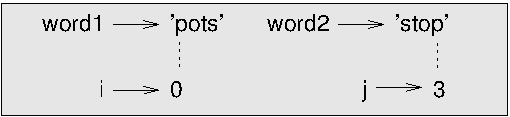
\includegraphics[scale=0.8]{figs/state4.pdf}}
\caption{State diagram.}
\label{fig.state4}
\end{figure}


I took a little license by arranging the variables in the frame
and adding dotted lines to show that the values of {\tt i} and
{\tt j} indicate characters in {\tt word1} and {\tt word2}.

我安排了框图中变量的位置并且增加了虚线展示{\tt i}和{\tt j}的值来指明
{\tt word1}和{\tt word2}中的字符。

\begin{exercise}
\label{isreverse}

Starting with this diagram, execute the program on paper, changing the
values of {\tt i} and {\tt j} during each iteration.  Find and fix the
second error in this function.

\end{exercise}



\section{Glossary 术语}

\begin{description}

\item[object(对象):] Something a variable can refer to.  For now,
you can use ``object'' and ``value'' interchangeably.
\index{object}

\item[sequence(序列):] An ordered set; that is, a set of
values where each value is identified by an integer index.
\index{sequence}

\item[item(项):] One of the values in a sequence.
\index{item}

\item[index(索引):] An integer value used to select an item in
a sequence, such as a character in a string.
\index{index}

\item[slice(切片):] A part of a string specified by a range of indices.
\index{slice}

\item[empty string(空字符串):] A string with no characters and length 0, represented
by two quotation marks.
\index{empty string}

\item[immutable(不可变的):] The property of a sequence whose items cannot
be assigned.
\index{immutability}

\item[traverse(遍历):] To iterate through the items in a sequence,
performing a similar operation on each.
\index{traversal}

\item[search(搜索):] A pattern of traversal that stops
when it finds what it is looking for.
\index{search pattern}
\index{pattern!search}

\item[counter(计数器):] A variable used to count something, usually initialized
to zero and then incremented.
\index{counter}

\item[method(方法):] A function that is associated with an object and called
using dot notation.
\index{method}

\item[invocation(调用):] A statement that calls a method.
\index{invocation}

\end{description}


\section{Exercises}

\begin{exercise}
\index{step size}
\index{slice operator}
\index{operator!slice}

A string slice can take a third index that specifies the ``step
size;'' that is, the number of spaces between successive characters.
A step size of 2 means every other character; 3 means every third,
etc.

\begin{verbatim}
>>> fruit = 'banana'
>>> fruit[0:5:2]
'bnn'
\end{verbatim}

A step size of -1 goes through the word backwards, so
the slice \verb"[::-1]" generates a reversed string.
\index{palindrome}

Use this idiom to write a one-line version of \verb"is_palindrome"
from Exercise~\ref{palindrome}.
\end{exercise}


\begin{exercise}

The following functions are all {\em intended} to check whether a
string contains any lowercase letters, but at least some of them are
wrong.  For each function, describe what the function actually does
(assuming that the parameter is a string).

\begin{verbatim}
def any_lowercase1(s):
    for c in s:
        if c.islower():
            return True
        else:
            return False

def any_lowercase2(s):
    for c in s:
        if 'c'.islower():
            return 'True'
        else:
            return 'False'

def any_lowercase3(s):
    for c in s:
        flag = c.islower()
    return flag

def any_lowercase4(s):
    flag = False
    for c in s:
        flag = flag or c.islower()
    return flag

def any_lowercase5(s):
    for c in s:
        if not c.islower():
            return False
    return True
\end{verbatim}

\end{exercise}


\begin{exercise}
\index{letter rotation}
\index{rotation, letter}

\label{exrotate}
ROT13 is a weak form of encryption that involves ``rotating'' each
letter in a word by 13 places.  To rotate a letter means
to shift it through the alphabet, wrapping around to the beginning if
necessary, so 'A' shifted by 3 is 'D' and 'Z' shifted by 1 is 'A'.

Write a function called \verb"rotate_word"
that takes a string and an integer as parameters, and that returns
a new string that contains the letters from the original string
``rotated'' by the given amount.  

For example, ``cheer'' rotated by 7 is ``jolly'' and ``melon'' rotated
by -10 is ``cubed''.  

%For example ``sleep''
%rotated by 9 is ``bunny'' and ``latex'' rotated by 7 is ``shale''.

You might want to use the built-in functions {\tt ord}, which converts
a character to a numeric code, and {\tt chr}, which converts numeric
codes to characters.

Potentially offensive jokes on the Internet are sometimes encoded
in ROT13.  If you are not easily offended, find and decode some
of them.  Solution: \url{http://thinkpython.com/code/rotate.py}.

\end{exercise}


\chapter{Case study: word play 案例分析:word play}

\section{Reading word lists 读取单词列表}
\label{wordlist}

For the exercises in this chapter we need a list of English words.
There are lots of word lists available on the Web, but the one most
suitable for our purpose is one of the word lists collected and
contributed to the public domain by Grady Ward as part of the Moby
lexicon project (see \url{http://wikipedia.org/wiki/Moby_Project}).  It
is a list of 113,809 official crosswords; that is, words that are
considered valid in crossword puzzles and other word games.  In the
Moby collection, the filename is {\tt 113809of.fic}; you can download
a copy, with the simpler name {\tt words.txt}, from
\url{http://thinkpython.com/code/words.txt}.
\index{Moby Project}
\index{crosswords}

对于本章的习题,我们需要一个英语单词的列表。
互联网上有许多单词列表,但是最适合我们目的之一的列表是由
Grady Ward收集并贡献给公众的,并成为Moby词典项目的一部分
(见:\url{http://wikipedia.org/wiki/Moby_Project})。
它是一个由113,809个填字游戏单词组成的列表,
也就是在填字游戏以及其它文字有戏中被认为合理的单词。
在Moby集合中,文件名是{\tt 113809of.fic},
你可以从\url{http://thinkpython.com/code/words.txt}下载一个拷贝,
其使用了一个简化的名字{\tt words.txt}。

This file is in plain text, so you can open it with a text
editor, but you can also read it from Python.  The built-in
function {\tt open} takes the name of the file as a parameter
and returns a {\bf file object} you can use to read the file.
\index{open function}
\index{function!open}
\index{plain text}
\index{text!plain}
\index{object!file}
\index{file object}

该文件是纯文本,所以你可以用一个文本编辑器打开它,
但是你也可以从Python中读它。
内建函数{\tt open}接受文件名作为形参,并返回一个
{\bf 文件对象(file object)},你可以使用它读取该文件。

\begin{verbatim}
>>> fin = open('words.txt')
>>> print fin
<open file 'words.txt', mode 'r' at 0xb7f4b380>
\end{verbatim}
%
{\tt fin} is a common name for a file object used for
input.  Mode \verb"'r'" indicates that this file is open for
reading (as opposed to \verb"'w'" for writing).
\index{readline method}
\index{method!readline}

{\tt fin}是输入文件对象的一个常用名。
模式\verb"'r'"表明该文件为了读取而打开
(相反,\verb"'w'"是为了写)。

The file object provides several methods for reading, including
{\tt readline}, which reads characters from the file
until it gets to a newline and returns the result as a
string:

该文件对象为读取提供了几个方法,包括{\tt readline},
其从文件中读取字符直到到达新行并将结果作为字符串返回:

\begin{verbatim}
>>> fin.readline()
'aa\r\n'
\end{verbatim}
%
The first word in this particular list is ``aa,'' which is a kind of
lava.  The sequence \verb"\r\n" represents two whitespace characters,
a carriage return and a newline, that separate this word from the
next.

在此列表中,第一个单词是``aa'',它是一种岩浆。
序列\verb"\r\n"代表两个空白字符,回车和换行,
其将此单词和下一个分开。

The file object keeps track of where it is in the file, so
if you call {\tt readline} again, you get the next word:

此文件对象跟踪它在文件中的位置,
所以如果你再次调用{\tt readline},你获得下一个单词:

\begin{verbatim}
>>> fin.readline()
'aah\r\n'
\end{verbatim}
%
The next word is ``aah,'' which is a perfectly legitimate
word, so stop looking at me like that.
Or, if it's the whitespace that's bothering you,
we can get rid of it with the string method {\tt strip}:
\index{strip method}
\index{method!strip}

下一个单词是``aah'',它是一个完全合法的单词,
所以不要那样看我。
或者,如果空格困扰了你,我们可以用字符串方法{\tt strip}删掉它:

\begin{verbatim}
>>> line = fin.readline()
>>> word = line.strip()
>>> print word
aahed
\end{verbatim}
%
You can also use a file object as part of a {\tt for} loop.
This program reads {\tt words.txt} and prints each word, one
per line:
\index{open function}
\index{function!open}

你也可以将文件对象用做{\tt for}循环的一部分。
此程序读取{\tt words.txt}并打印每个单词,每行一个:

\begin{verbatim}
fin = open('words.txt')
for line in fin:
    word = line.strip()
    print word
\end{verbatim}
%

\begin{exercise}

Write a program that reads {\tt words.txt} and prints only the
words with more than 20 characters (not counting whitespace).
\index{whitespace}

\end{exercise}


\section{Exercises 习题}

There are solutions to these exercises in the next section.
You should at least attempt each one before you read the solutions.

下一节有这些习题的答案。
在你看这些答案之前,应该至少试这解决一下每个题目。

\begin{exercise}

In 1939 Ernest Vincent Wright published a 50,000 word novel called
{\em Gadsby} that does not contain the letter ``e.''  Since ``e'' is
the most common letter in English, that's not easy to do.

1939年,Ernest Vincent Wright发表了一本名为{\em Gadsby}的小说,
该小说不包括字母``e''。由于``e''是最常用的英文字母,因此这并容易做到。

In fact, it is difficult to construct a solitary thought without using
that most common symbol.  It is slow going at first, but with caution
and hours of training you can gradually gain facility.

事实上,不使用这个最常用的符号是很难的。
开始进展缓慢,但是经过认真的长时间的训练,你可以逐渐地熟练。

All right, I'll stop now.

好的,现在我将停下。

Write a function called \verb"has_no_e" that returns {\tt True} if
the given word doesn't have the letter ``e'' in it.

写一个称作\verb"has_no_e"的函数,如果给定的单词中不包含字母``e'',其返回{\tt True}

Modify your program from the previous section to print only the words
that have no ``e'' and compute the percentage of the words in the list
have no ``e.''
\index{lipogram}

修改你前面小节中的程序以只打印不包含``e''的单词,
并且计算列表中不含``e''的单词的百分百。

\end{exercise}


\begin{exercise} 

Write a function named {\tt avoids}
that takes a word and a string of forbidden letters, and
that returns {\tt True} if the word doesn't use any of the forbidden
letters.

写一个名为{\tt avoids}的函数,接受一个单词和一个禁止字母字符串,
如果单词中不包含任意禁止字母,则返回{\tt True} 。

Modify your program to prompt the user to enter a string
of forbidden letters and then print the number of words that
don't contain any of them.
Can you find a combination of 5 forbidden letters that
excludes the smallest number of words?

修改你的程序,提示用户输入一个禁止字母字符串然后打印不包含它们的单词的数量。
你能找到一个5个禁止字母的组合,使得其不包含最小单词数目么?

\end{exercise}



\begin{exercise}

Write a function named \verb"uses_only" that takes a word and a
string of letters, and that returns {\tt True} if the word contains
only letters in the list.  Can you make a sentence using only the
letters {\tt acefhlo}?  Other than ``Hoe alfalfa?''

写一个名为\verb"uses_only"的函数,其接受一个单词和一个字符串,
如果该单词只包括此字符串中的字母,则返回{\tt True}。
你能只是用字母{\tt acefhlo}造一个句子么?
除了``Hoe alfalfa''外。

\end{exercise}


\begin{exercise} 

Write a function named \verb"uses_all" that takes a word and a
string of required letters, and that returns {\tt True} if the word
uses all the required letters at least once.  How many words are there
that use all the vowels {\tt aeiou}?  How about {\tt aeiouy}?

\end{exercise}


\begin{exercise}

Write a function called \verb"is_abecedarian" that returns
{\tt True} if the letters in a word appear in alphabetical order
(double letters are ok).  
How many abecedarian words are there?

写一个名为\verb"is_abecedarian"的函数,
如果单词中的字母以字母表的顺序出现(允许重复字母),则返回{\tt True} 。
有多少个abecedarian单词?

\index{abecedarian}

\end{exercise}


%\begin{exercise}
%\label{palindrome}
%A palindrome is a word that reads the same
%forward and backward, like ``rotator'' and ``noon.''
%Write a boolean function named \verb"is_palindrome" that
%takes a string as a parameter and returns {\tt True} if it is
%a palindrome.

%Modify your program from the previous section to print all
%of the palindromes in the word list and then print the total
%number of palindromes.
%\end{exercise}



\section{Search 搜索}
\index{search pattern}
\index{pattern!search}

All of the exercises in the previous section have something
in common; they can be solved with the search pattern we saw
in Section~\ref{find}.  The simplest example is:

前一节的所有习题有一个共性,它们可以用我们在\ref{find}节中看到的搜索模式解决。
最简单的例子是:

\begin{verbatim}
def has_no_e(word):
    for letter in word:
        if letter == 'e':
            return False
    return True
\end{verbatim}
%
The {\tt for} loop traverses the characters in {\tt word}.  If we find
the letter ``e'', we can immediately return {\tt False}; otherwise we
have to go to the next letter.  If we exit the loop normally, that
means we didn't find an ``e'', so we return {\tt True}.
\index{traversal}

{\tt for}循环遍历{\tt word}中的字符。
如果我们找到字母``e'',那么我们可以马上返回{\tt False};
否则我们不得不到下一个字母。
如果我们正常停止循环,这意味着我们没有找到一个``e'',
所以我们返回{\tt True}。 

% Removing this because we haven't seen the in operator yet.
%\index{in operator}
%\index{operator!in}

%You could write this function more concisely using the {\tt in}
%operator, but I started with this version because it 
%demonstrates the logic of the search pattern.
\index{generalization}

{\tt avoids} is a more general version of \verb"has_no_e" but it
has the same structure:

{\tt avoids}是\verb"has_no_e"的更一般的版本,但是它有相同的结构:

\begin{verbatim}
def avoids(word, forbidden):
    for letter in word:
        if letter in forbidden:
            return False
    return True
\end{verbatim}
%
We can return {\tt False} as soon as we find a forbidden letter;
if we get to the end of the loop, we return {\tt True}.

一旦我们找到一个禁止字母,我们返回{\tt False};
如果我们到达循环结尾,我们返回{\tt True}。

\verb"uses_only" is similar except that the sense of the condition
is reversed:

除了条件的意思相反外,\verb"uses_only"也是相似的:

\begin{verbatim}
def uses_only(word, available):
    for letter in word: 
        if letter not in available:
            return False
    return True
\end{verbatim}
%
Instead of a list of forbidden letters, we have a list of available
letters.  If we find a letter in {\tt word} that is not in
{\tt available}, we can return {\tt False}.

不是有一个禁止字母的列表,而是我们有一个允许字母的列表。
如果我们在{\tt word}中找到一个不在{\tt available}中的字母,
我们可以返回{\tt False}

\verb"uses_all" is similar except that we reverse the role
of the word and the string of letters:

除了我们翻转了单词和字母字符串的角色外,\verb"uses_all"也类似:

\begin{verbatim}
def uses_all(word, required):
    for letter in required: 
        if letter not in word:
            return False
    return True
\end{verbatim}
%
Instead of traversing the letters in {\tt word}, the loop
traverses the required letters.  If any of the required letters
do not appear in the word, we can return {\tt False}.
\index{traversal}

不是在{\tt word}中遍历字母,该循环遍历需要的字母。
如果任何需要的字母没出现在单词中,
则我们返回{\tt False}。

If you were really thinking like a computer scientist, you would
have recognized that \verb"uses_all" was an instance of a
previously-solved problem, and you would have written:

如果你真的像计算机科学家一样思考,
你可能已经意识到\verb"uses_all"是前面已经解决的问题的一个实例,
你可能会写成:

\begin{verbatim}
def uses_all(word, required):
    return uses_only(required, word)
\end{verbatim}
%
This is an example of a program development method called {\bf problem
recognition}, which means that you recognize the problem you are
working on as an instance of a previously-solved problem, and apply a
previously-developed solution.
\index{problem recognition}
\index{development plan!problem recognition}

这是一个被称作{\bf 问题识别(problem recognition)}的程序开发方法的实例,
意思是你将正在解决的问题看做是之前已经解决的问题的一个实例,
并用用之前开发的解决方案。

\section{Looping with indices 使用索引的循环}
\index{looping!with indices}
\index{index!looping with}

I wrote the functions in the previous section with {\tt for}
loops because I only needed the characters in the strings; I didn't
have to do anything with the indices.

前一节我用{\tt for}循环写函数,因为我只需要字符串中的字符,
我不必用索引做任何事情。

For \verb"is_abecedarian" we have to compare adjacent letters,
which is a little tricky with a {\tt for} loop:

对于\verb"is_abecedarian",我们必须比较邻接的字母,
这是一个用{\tt for}循环的小技巧。

\begin{verbatim}
def is_abecedarian(word):
    previous = word[0]
    for c in word:
        if c < previous:
            return False
        previous = c
    return True
\end{verbatim}


An alternative is to use recursion:

另外的替代方法是使用递归:

\begin{verbatim}
def is_abecedarian(word):
    if len(word) <= 1:
        return True
    if word[0] > word[1]:
        return False
    return is_abecedarian(word[1:])
\end{verbatim}

Another option is to use a {\tt while} loop:

另一个选择是使用{\tt while}循环:

\begin{verbatim}
def is_abecedarian(word):
    i = 0
    while i < len(word)-1:
        if word[i+1] < word[i]:
            return False
        i = i+1
    return True
\end{verbatim}
%
The loop starts at {\tt i=0} and ends when {\tt i=len(word)-1}.  Each
time through the loop, it compares the $i$th character (which you can
think of as the current character) to the $i+1$th character (which you
can think of as the next).

循环起始于{\tt i=0},终止于{\tt i=len(word)-1}。
每次循环比较第$i$个字符(我们可以将其认为是当前字符)
和第$i+1$个字符(我们可以将其认为是下一个字符)。

If the next character is less than (alphabetically before) the current
one, then we have discovered a break in the abecedarian trend, and
we return {\tt False}.

如果下一个字符比当前的小(字母序靠前),
那么我们在递增趋势中找到了停止点并返回{\tt False}。

If we get to the end of the loop without finding a fault, then the
word passes the test.  To convince yourself that the loop ends
correctly, consider an example like \verb"'flossy'".  The
length of the word is 6, so
the last time the loop runs is when {\tt i} is 4, which is the
index of the second-to-last character.  On the last iteration,
it compares the second-to-last character to the last, which is
what we want.
\index{palindrome}

如果到达循环结束,我们也没有找到一点错误,那么该单词通过测试。
为了说服你自己循环正确的结束了,考虑一个类似\verb"'flossy'"的例子。
其长度为6,因此最后一次循环运行时,{\tt i}是4,这是倒数第2个字符。
最后一次迭代,它比较倒数第二个和最后一个字符,这正是我们希望的。

Here is a version of \verb"is_palindrome" (see
Exercise~\ref{palindrome}) that uses two indices; one starts at the
beginning and goes up; the other starts at the end and goes down.

这是\verb"is_palindrome"的一个版本(见练习\ref{palindrome}),
其使用两个索引,一个从最前面开始并往前上,
另一个从最后面开始并往下走。

\begin{verbatim}
def is_palindrome(word):
    i = 0
    j = len(word)-1

    while i<j:
        if word[i] != word[j]:
            return False
        i = i+1
        j = j-1

    return True
\end{verbatim}

Or, if you noticed that this is an instance of a previously-solved
problem, you might have written:

或者,如果你注意到这是一个之前已经解决问题的一个实例,
你可能已经写成:

\begin{verbatim}
def is_palindrome(word):
    return is_reverse(word, word)
\end{verbatim}
\index{problem recognition}
\index{development plan!problem recognition}

Assuming you did Exercise~\ref{isreverse}.

假设你做了练习\ref{isreverse}。


\section{Debugging 调试}
\index{debugging}
\index{testing!is hard}
\index{program testing}

Testing programs is hard.  The functions in this chapter are
relatively easy to test because you can check the results by hand.
Even so, it is somewhere between difficult and impossible to choose a
set of words that test for all possible errors.

测试程序很难。本章的函数相对容易测试,因为你可以手工检查结果。
即使这样,选择一个单词的集合来测试所有可能的错误,
在某些方面也是介于困难和不可能的。

Taking \verb"has_no_e" as an example, there are two obvious
cases to check: words that have an 'e' should return {\tt False};
words that don't should return {\tt True}.  You should have no
trouble coming up with one of each.

例如\verb"has_no_e",有两个明显的用例需要检查:
含有`e'的单词应该返回{\tt False},不含的单词应该返回{\tt True}。
对任何一个你应该都不会有麻烦。

Within each case, there are some less obvious subcases.  Among the
words that have an ``e,'' you should test words with an ``e'' at the
beginning, the end, and somewhere in the middle.  You should test long
words, short words, and very short words, like the empty string.  The
empty string is an example of a {\bf special case}, which is one of
the non-obvious cases where errors often lurk.
\index{special case}

在每个用例中,还有一些不明显的子用例。
在含有``e''的单词中,你应该测试``e''在开始、结尾以及在中间的单词。
你应该测试长单词、短单词以及非常短的单词,如空字符串。
空字符串是{\bf 特殊用例(special case)}的一个例子,
其是一个经常隐藏错误的不明显的用例。

In addition to the test cases you generate, you can also test
your program with a word list like {\tt words.txt}.  By scanning
the output, you might be able to catch errors, but be careful:
you might catch one kind of error (words that should not be
included, but are) and not another (words that should be included,
but aren't).

除了你生成的测试用例,你也可以用一个类似{\tt words.txt}的单词列表测试你的程序。
通过扫描输出,你可能会捕获错误,但是请小心:
你可能捕获一类错误(包括了不应该包括的单词)
但不会捕获另一类错误(没有包括应该包括的单词)。

In general, testing can help you find bugs, but it is not easy to
generate a good set of test cases, and even if you do, you can't
be sure your program is correct.
\index{testing!and absence of bugs}

一般来讲,测试能帮助你找到错误,
但是生成好的测试用例的集合并不容易,
并且即便你做到了,你仍然不能保证你的程序是正确的。

According to a legendary computer scientist:

据一个传奇计算机科学家所说:

\begin{quote}
Program testing can be used to show the presence of bugs, but never to
show their absence!

程序测试能被用于展现错误的存在,但是从不会显示其不存在!

--- Edsger W. Dijkstra
\end{quote}
\index{Dijkstra, Edsger}


\section{Glossary 术语表}

\begin{description}

\item[file object(文件对象):] A value that represents an open file.
\index{file object}
\index{object!file}

\item[problem recognition(问题识别):] A way of solving a problem by
expressing it as an instance of a previously-solved problem.
\index{problem recognition}

\item[special case(特殊用例):] A test case that is atypical or non-obvious
(and less likely to be handled correctly).
\index{special case}

\end{description}


\section{Exercises}

\begin{exercise}
\index{Car Talk}
\index{Puzzler}
\index{double letters}

This question is based on a Puzzler that was broadcast on the radio
program {\em Car Talk} 
(\url{http://www.cartalk.com/content/puzzler/transcripts/200725}):

\begin{quote}
Give me a word with three consecutive double letters. I'll give you a
couple of words that almost qualify, but don't. For example, the word
committee, c-o-m-m-i-t-t-e-e. It would be great except for the `i' that
sneaks in there. Or Mississippi: M-i-s-s-i-s-s-i-p-p-i. If you could
take out those i's it would work. But there is a word that has three
consecutive pairs of letters and to the best of my knowledge this may
be the only word. Of course there are probably 500 more but I can only
think of one. What is the word?
\end{quote}

Write a program to find it.  Solution: \url{http://thinkpython.com/code/cartalk1.py}.

\end{exercise}


\begin{exercise}
Here's another {\em Car Talk}
Puzzler (\url{http://www.cartalk.com/content/puzzler/transcripts/200803}):
\index{Car Talk}
\index{Puzzler}
\index{odometer}
\index{palindrome}

\begin{quote}
``I was driving on the highway the other day and I happened to
notice my odometer. Like most odometers, it shows six digits,
in whole miles only. So, if my car had 300,000
miles, for example, I'd see 3-0-0-0-0-0.

``Now, what I saw that day was very interesting. I noticed that the
last 4 digits were palindromic; that is, they read the same forward as
backward. For example, 5-4-4-5 is a palindrome, so my odometer
could have read 3-1-5-4-4-5.

``One mile later, the last 5 numbers were palindromic. For example, it
could have read 3-6-5-4-5-6.  One mile after that, the middle 4 out of
6 numbers were palindromic.  And you ready for this? One mile later,
all 6 were palindromic!

``The question is, what was on the odometer when I first looked?''
\end{quote}

Write a Python program that tests all the six-digit numbers and prints
any numbers that satisfy these requirements.  
Solution: \url{http://thinkpython.com/code/cartalk2.py}.

\end{exercise}


\begin{exercise}
Here's another {\em Car Talk} Puzzler you can solve with a
search (\url{http://www.cartalk.com/content/puzzler/transcripts/200813}):
\index{Car Talk}
\index{Puzzler}
\index{palindrome}

\begin{quote}
``Recently I had a visit with my mom and we realized that
the two digits that make up my age when reversed resulted in her
age. For example, if she's 73, I'm 37. We wondered how often this has
happened over the years but we got sidetracked with other topics and
we never came up with an answer.

``When I got home I figured out that the digits of our ages have been
reversible six times so far. I also figured out that if we're lucky it
would happen again in a few years, and if we're really lucky it would
happen one more time after that. In other words, it would have
happened 8 times over all. So the question is, how old am I now?''

\end{quote}

Write a Python program that searches for solutions to this Puzzler.
Hint: you might find the string method {\tt zfill} useful.

Solution: \url{http://thinkpython.com/code/cartalk3.py}.

\end{exercise}



\chapter{Lists 列表}

\section{A list is a sequence 列表是一个序列}
\label{sequence}

Like a string, a {\bf list} is a sequence of values.  In a string, the
values are characters; in a list, they can be any type.  The values in
a list are called {\bf elements} or sometimes {\bf items}.
\index{list}
\index{type!list}
\index{element}
\index{sequence}
\index{item}

像字符串一样,一个{\bf 列表(list)}是值的序列。
在字符串中,值是字符;在列表中,它们可以是任意值。
列表中的值被称作{\bf 元素(elements)}或者{\bf 项(items)}。

There are several ways to create a new list; the simplest is to
enclose the elements in square brackets (\verb"[" and \verb"]"):

有几种方法生成一个新的列表;
最简单的是把这些元素括在方括号中(\verb"[" and \verb"]"):

\begin{verbatim}
[10, 20, 30, 40]
['crunchy frog', 'ram bladder', 'lark vomit']
\end{verbatim}
%
The first example is a list of four integers.  The second is a list of
three strings.  The elements of a list don't have to be the same type.
The following list contains a string, a float, an integer, and
(lo!) another list:

第一个例子是一个四个整数的列表。第二个是三个字符串。
列表的元素不必是相同的类型。
下面的列表包括一个字符串、一个浮点数、一个整数和(什么!)另一个列表:

\begin{verbatim}
['spam', 2.0, 5, [10, 20]]
\end{verbatim}
%
A list within another list is {\bf nested}.
\index{nested list}
\index{list!nested}

在另一个列表中的列表是{\bf 嵌套(nested)}。

A list that contains no elements is
called an empty list; you can create one with empty
brackets, \verb"[]".
\index{empty list}
\index{list!empty}

不包括任何元素的列表被称作空列表。
你可以用空括号,\verb"[]",生成一个空列表。

As you might expect, you can assign list values to variables:

如你所期望的,你可以将列表的值赋给变量:

\begin{verbatim}
>>> cheeses = ['Cheddar', 'Edam', 'Gouda']
>>> numbers = [17, 123]
>>> empty = []
>>> print cheeses, numbers, empty
['Cheddar', 'Edam', 'Gouda'] [17, 123] []
\end{verbatim}
%
\index{assignment}


\section{Lists are mutable 列表是可变的}
\label{mutable}
\index{list!element}
\index{access}
\index{index}
\index{bracket operator}
\index{operator!bracket}

The syntax for accessing the elements of a list is the same as for
accessing the characters of a string---the bracket operator.  The
expression inside the brackets specifies the index.  Remember that the
indices start at 0:

访问列表元素的语法和访问字符串的字符的语法相同---括号运算符。
括号内的表达式制定索引。记住索引以0开始:

\begin{verbatim}
>>> print cheeses[0]
Cheddar
\end{verbatim}
%
Unlike strings, lists are mutable.  When the bracket operator appears
on the left side of an assignment, it identifies the element of the
list that will be assigned.
\index{mutability}

和字符串不同,列表是可变的。
当括号运算符出现在赋值的左侧时,它识别出将被赋值的列表的元素。

\begin{verbatim}
>>> numbers = [17, 123]
>>> numbers[1] = 5
>>> print numbers
[17, 5]
\end{verbatim}
%
The one-eth element of {\tt numbers}, which
used to be 123, is now 5.
\index{index!starting at zero}
\index{zero, index starting at}

{\tt numbers}的第一个元素,过去是123,现在是5.

You can think of a list as a relationship between indices and
elements.  This relationship is called a {\bf mapping}; each index
``maps to'' one of the elements.  Figure~\ref{fig.liststate} shows 
the state diagram for {\tt
cheeses}, {\tt numbers} and {\tt empty}:
\index{state diagram}
\index{diagram!state}
\index{mapping}

你可以将列表看成索引和元素之间的关系。
此关系被称作{\bf 映射(mapping)},每个索引``映射''到一个元素。
图\ref{fig.liststate}展示了{\tt cheeses}、{\tt numbers}和{\tt empty}的栈图:

\begin{figure}
\centerline
{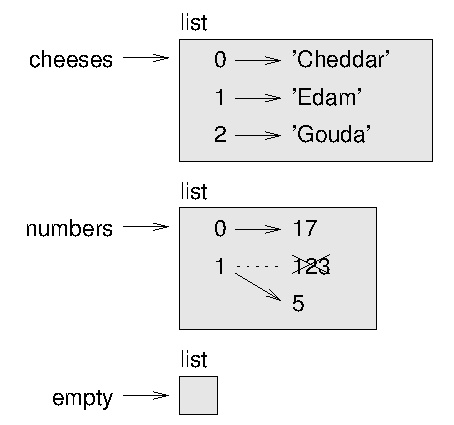
\includegraphics[scale=0.8]{figs/liststate.pdf}}
\caption{State diagram.}
\label{fig.liststate}
\end{figure}

Lists are represented by boxes with the word ``list'' outside
and the elements of the list inside.  {\tt cheeses} refers to
a list with three elements indexed 0, 1 and 2.
{\tt numbers} contains two elements; the diagram shows that the
value of the second element has been reassigned from 123 to 5.
{\tt empty} refers to a list with no elements.
\index{item assignment}
\index{assignment!item}

列表用盒子表示,外面写着``list''里面是元素。
{\tt cheeses}指向一个有三个元素的列表,索引是0、1和2.
{\tt numbers}包括两个元素,此图显示第二个元素的值已经被从123重新赋成了5.
{\tt empty}指向一个没有任何元素的列表。

List indices work the same way as string indices:

列表索引和字符串索引作用相同:

\begin{itemize}

\item Any integer expression can be used as an index.

任何整数表达式可以被用作索引。

\item If you try to read or write an element that does not exist, you
get an {\tt IndexError}.
\index{exception!IndexError}
\index{IndexError}

如果你试图读或写一个不存在的元素,你获得一个{\tt IndexError}。

\item If an index has a negative value, it counts backward from the
end of the list.

如果一个索引是一个负值,它从列表的结尾往回数。

\end{itemize}
\index{list!index}

\index{list!membership}
\index{membership!list}
\index{in operator}
\index{operator!in}

The {\tt in} operator also works on lists.

{\tt in}运算符也可以用于列表。

\begin{verbatim}
>>> cheeses = ['Cheddar', 'Edam', 'Gouda']
>>> 'Edam' in cheeses
True
>>> 'Brie' in cheeses
False
\end{verbatim}


\section{Traversing a list 遍历一个列表}
\index{list!traversal}
\index{traversal!list}
\index{for loop}
\index{loop!for}
\index{statement!for}

The most common way to traverse the elements of a list is
with a {\tt for} loop.  The syntax is the same as for strings:

遍历一个列表元素的最常用方法是用{\tt for}循环。
语法和遍历字符串相同:

\begin{verbatim}
for cheese in cheeses:
    print cheese
\end{verbatim}
%
This works well if you only need to read the elements of the
list.  But if you want to write or update the elements, you
need the indices.  A common way to do that is to combine
the functions {\tt range} and {\tt len}:
\index{looping!with indices}
\index{index!looping with}

如果你只想读列表的元素,这工作的很好。
但是如果你想写或者更新元素,那么你需要索引。
一个常用的方法是组合{\tt range}和{\tt len}函数:

\begin{verbatim}
for i in range(len(numbers)):
    numbers[i] = numbers[i] * 2
\end{verbatim}
%
This loop traverses the list and updates each element.  {\tt len}
returns the number of elements in the list.  {\tt range} returns
a list of indices from 0 to $n-1$, where $n$ is the length of
the list.  Each time through the loop {\tt i} gets the index
of the next element.  The assignment statement in the body uses
{\tt i} to read the old value of the element and to assign the
new value.
\index{item update}
\index{update!item}

该循环遍历列表并更新每个元素。
{\tt len}返回列表中元素的数目。
{\tt range}返回一个从0到$n-1$的索引的列表,
其中$n$是列表的长度。
循环{\tt i}每次获得下一个元素的索引。
循环体内的赋值语句使用{\tt i}来读旧的元素的值并赋予新值。

A {\tt for} loop over an empty list never executes the body:
空列表上的{\tt for}循环从不执行循环体:

\begin{verbatim}
for x in []:
    print 'This never happens.'
\end{verbatim}
%
Although a list can contain another list, the nested
list still counts as a single element.  The length of this list is
four:
\index{nested list}
\index{list!nested}

虽然一个列表可以包括另一个列表,
但是嵌套的列表仍然像一个单一元素一样计数。
该列表的长度是4:

\begin{verbatim}
['spam', 1, ['Brie', 'Roquefort', 'Pol le Veq'], [1, 2, 3]]
\end{verbatim}



\section{List operations 列表运算}
\index{list!operation}

The {\tt +} operator concatenates lists:
\index{concatenation!list}
\index{list!concatenation}

{\tt +}运算符叠加列表:

\begin{verbatim}
>>> a = [1, 2, 3]
>>> b = [4, 5, 6]
>>> c = a + b
>>> print c
[1, 2, 3, 4, 5, 6]
\end{verbatim}
%
Similarly, the {\tt *} operator repeats a list a given number of times:
\index{repetition!list}
\index{list!repetition}

类似地,{\tt *}运算符重复列表给定次数:

\begin{verbatim}
>>> [0] * 4
[0, 0, 0, 0]
>>> [1, 2, 3] * 3
[1, 2, 3, 1, 2, 3, 1, 2, 3]
\end{verbatim}
%
The first example repeats {\tt [0]} four times.  The second example
repeats the list {\tt [1, 2, 3]} three times.

第一个例子重复{\tt [0]} 4次。
第二个例子重复列表{\tt [1, 2, 3]} 3次。


\section{List slices 列表切片}
\index{slice operator}
\index{operator!slice}
\index{index!slice}
\index{list!slice}
\index{slice!list}

The slice operator also works on lists:

切片运算符也能用于列表:

\begin{verbatim}
>>> t = ['a', 'b', 'c', 'd', 'e', 'f']
>>> t[1:3]
['b', 'c']
>>> t[:4]
['a', 'b', 'c', 'd']
>>> t[3:]
['d', 'e', 'f']
\end{verbatim}
%
If you omit the first index, the slice starts at the beginning.
If you omit the second, the slice goes to the end.  So if you
omit both, the slice is a copy of the whole list.
\index{list!copy}
\index{slice!copy}
\index{copy!slice}

如果你不写第一个索引,切片起始于开始。
如果不写第二个,切片直到结束。
所以,如果你两个都不写,切片拷贝整个列表。

\begin{verbatim}
>>> t[:]
['a', 'b', 'c', 'd', 'e', 'f']
\end{verbatim}
%
Since lists are mutable, it is often useful to make a copy
before performing operations that fold, spindle or mutilate
lists.
\index{mutability}

既然列表是可变的,那么在对列表进行操作之前拷贝它通常很有用。

A slice operator on the left side of an assignment
can update multiple elements:
\index{slice!update}
\index{update!slice}

赋值语句左侧的切片运算符可以更新多个元素:

\begin{verbatim}
>>> t = ['a', 'b', 'c', 'd', 'e', 'f']
>>> t[1:3] = ['x', 'y']
>>> print t
['a', 'x', 'y', 'd', 'e', 'f']
\end{verbatim}
%

% You can add elements to a list by squeezing them into an empty
% slice:

% % \begin{verbatim}
% >>> t = ['a', 'd', 'e', 'f']
% >>> t[1:1] = ['b', 'c']
% >>> print t
% ['a', 'b', 'c', 'd', 'e', 'f']
% \end{verbatim}
% \afterverb
%
% And you can remove elements from a list by assigning the empty list to
% them:

% % \begin{verbatim}
% >>> t = ['a', 'b', 'c', 'd', 'e', 'f']
% >>> t[1:3] = []
% >>> print t
% ['a', 'd', 'e', 'f']
% \end{verbatim}
% \afterverb
%
% But both of those operations can be expressed more clearly
% with list methods.


\section{List methods 列表方法}
\index{list!method}
\index{method, list}

Python provides methods that operate on lists.  For example,
{\tt append} adds a new element to the end of a list:
\index{append method}
\index{method!append}

Python提供在列表上运算的方法。
例如{\tt append}在列表结尾增加一个新元素:

\begin{verbatim}
>>> t = ['a', 'b', 'c']
>>> t.append('d')
>>> print t
['a', 'b', 'c', 'd']
\end{verbatim}
%
{\tt extend} takes a list as an argument and appends all of
the elements:
\index{extend method}
\index{method!extend}

{\tt extend}将一个列表作为实参并追加所有的元素:

\begin{verbatim}
>>> t1 = ['a', 'b', 'c']
>>> t2 = ['d', 'e']
>>> t1.extend(t2)
>>> print t1
['a', 'b', 'c', 'd', 'e']
\end{verbatim}
%
This example leaves {\tt t2} unmodified.

此例不改变{\tt t2}。

{\tt sort} arranges the elements of the list from low to high:
\index{sort method}
\index{method!sort}

{\tt sort}从低到高排列列表的元素:

\begin{verbatim}
>>> t = ['d', 'c', 'e', 'b', 'a']
>>> t.sort()
>>> print t
['a', 'b', 'c', 'd', 'e']
\end{verbatim}
%
List methods are all void; they modify the list and return {\tt None}.
If you accidentally write {\tt t = t.sort()}, you will be disappointed
with the result.
\index{void method}
\index{method!void}
\index{None special value}
\index{special value!None}

列表方法都是无返回值的,它们修改列表并返回{\tt None}。
如果你偶然写了{\tt t = t.sort()},你将对结果很失望。


\section{Map, filter and reduce 映射、过滤和削减}

To add up all the numbers in a list, you can use a loop like this:

为了累加列表中的所有的数,你可以使用如下的循环:

% see add.py

\begin{verbatim}
def add_all(t):
    total = 0
    for x in t:
        total += x
    return total
\end{verbatim}
%
{\tt total} is initialized to 0.  Each time through the loop,
{\tt x} gets one element from the list.  The {\tt +=} operator
provides a short way to update a variable.  This 
{\bf augmented assignment statement}:
\index{update operator}
\index{operator!update}
\index{assignment!augmented}
\index{augmented assignment}

{\tt total}初始化为0。每次循环,{\tt x}从列表中获得一个元素。
{\tt +=}运算符提供了一个简化的方法来更新一个变量。
此{\bf 增量赋值语句(augmented assignment statement)}:

\begin{verbatim}
    total += x
\end{verbatim}
%
is equivalent to:

等价于:

\begin{verbatim}
    total = total + x
\end{verbatim}
%
As the loop executes, {\tt total} accumulates the sum of the
elements; a variable used this way is sometimes called an
{\bf accumulator}.
\index{accumulator!sum}

当循环执行时,{\tt total}累计元素的和,
这样使用的变量有时被称作一个{\bf 累加器(accumulator)}。

Adding up the elements of a list is such a common operation
that Python provides it as a built-in function, {\tt sum}:

累加一个列表的元素是如此通常的运算,
以至于Python为其提供了一个内建函数,{\tt sum}:

\begin{verbatim}
>>> t = [1, 2, 3]
>>> sum(t)
6
\end{verbatim}
%
An operation like this that combines a sequence of elements into
a single value is sometimes called {\bf reduce}.
\index{reduce pattern}
\index{pattern!reduce}
\index{traversal}

像这样将一序列元素组合成一个单一值的运算有时被称作{\bf 消减(reduce)}。

\begin{exercise}

Write a function called \verb"nested_sum" that takes a nested list
of integers and add up the elements from all of the nested lists.

\end{exercise}

Sometimes you want to traverse one list while building
another.  For example, the following function takes a list of strings
and returns a new list that contains capitalized strings:

有时,你想一边遍历一个列表,一边创建另一个。
例如,下面的函数接受一个字符串列表并返回一个新的包含大写字母字符串的列表:

\begin{verbatim}
def capitalize_all(t):
    res = []
    for s in t:
        res.append(s.capitalize())
    return res
\end{verbatim}
%
{\tt res} is initialized with an empty list; each time through
the loop, we append the next element.  So {\tt res} is another
kind of accumulator.
\index{accumulator!list}

{\tt res}用一个空列表初始化,循环每次追加下一个元素。
所以{\tt res}是另一类累加器。

An operation like \verb"capitalize_all" is sometimes called a {\bf
map} because it ``maps'' a function (in this case the method {\tt
capitalize}) onto each of the elements in a sequence.
\index{map pattern}
\index{pattern!map}
\index{filter pattern}
\index{pattern!filter}

类似\verb"capitalize_all"的运算有时被称作a {\bf 映射(map)},
因为它``映射''一个函数(此例中是{\tt capitalize}方法)到一个序列的每个元素上。

\begin{exercise}

Use \verb"capitalize_all" to write a function named \verb"capitalize_nested"
that takes a nested list of strings and returns a new nested list
with all strings capitalized.

\end{exercise}

Another common operation is to select some of the elements from
a list and return a sublist.  For example, the following
function takes a list of strings and returns a list that contains
only the uppercase strings:

另一个常见运算是从列表中选择一些元素并返回子列表。
例如,下面的函数接受一个字符串列表并返回只包含大写字母的字符串:

\begin{verbatim}
def only_upper(t):
    res = []
    for s in t:
        if s.isupper():
            res.append(s)
    return res
\end{verbatim}
%
{\tt isupper} is a string method that returns {\tt True} if
the string contains only upper case letters.

{\tt isupper}是一个字符串方法,
如果字符串只包含大写字母,其返回{\tt True}。

An operation like \verb"only_upper" is called a {\bf filter} because
it selects some of the elements and filters out the others.

类似\verb"only_upper"的运算被称作{\bf 过滤(filter)},
因为它选择一些元素并过滤掉其它的。

Most common list operations can be expressed as a combination
of map, filter and reduce.  Because these operations are
so common, Python provides language features to support them,
including the built-in function {\tt map} and an operator
called a ``list comprehension.''
\index{list!comprehension}

最通常的列表运算能被表示成映射、过滤和消减的组合。
因为这些运算如此通常,以至于Python提供了支持它们的语言特征,
包括内建函数{\tt map}以及一个被称作``列表理解''的操作符。

\begin{exercise}
\label{cumulative}
\index{cumulative sum}

Write a function that takes a list of numbers and returns the
cumulative sum; that is, a new list where the $i$th element
is the sum of the first $i+1$ elements from the original list.
For example, the cumulative sum of {\tt [1, 2, 3]} is
{\tt [1, 3, 6]}. 
\end{exercise}


\section{Deleting elements 删除元素}
\index{element deletion}
\index{deletion, element of list}

There are several ways to delete elements from a list.  If you
know the index of the element you want, you can use
{\tt pop}:
\index{pop method}
\index{method!pop}

有几种从列表中删除元素的方法。
如果你知道你想删除的元素的索引,你可以使用{\tt pop}:

\begin{verbatim}
>>> t = ['a', 'b', 'c']
>>> x = t.pop(1)
>>> print t
['a', 'c']
>>> print x
b
\end{verbatim}
%
{\tt pop} modifies the list and returns the element that was removed.
If you don't provide an index, it deletes and returns the
last element.

{\tt pop}改变列表并返回被删除的元素。
如果不提供索引,它删除并返回最后一个元素。

If you don't need the removed value, you can use the {\tt del}
operator:
\index{del operator}
\index{operator!del}

如果你不需要被删除的值,你可以使用{\tt del}运算符:

\begin{verbatim}
>>> t = ['a', 'b', 'c']
>>> del t[1]
>>> print t
['a', 'c']
\end{verbatim}
%

If you know the element you want to remove (but not the index), you
can use {\tt remove}:
\index{remove method}
\index{method!remove}

如果你知道你想删除的元素(但是不知道索引),
你可以使用{\tt remove}:

\begin{verbatim}
>>> t = ['a', 'b', 'c']
>>> t.remove('b')
>>> print t
['a', 'c']
\end{verbatim}
%
The return value from {\tt remove} is {\tt None}.
\index{None special value}
\index{special value!None}

{\tt remove}的返回值是{\tt None}。

To remove more than one element, you can use {\tt del} with
a slice index:

为了删除多余一个的元素,你可以使用{\tt del}和一个切片索引:

\begin{verbatim}
>>> t = ['a', 'b', 'c', 'd', 'e', 'f']
>>> del t[1:5]
>>> print t
['a', 'f']
\end{verbatim}
%
As usual, the slice selects all the elements up to, but not
including, the second index.

和通常一样,该切片选择所有高于,但是不包含第二个索引的元素。

\begin{exercise}

Write a function called \verb"middle" that takes a list and
returns a new list that contains all but the first and last
elements.  So \verb"middle([1,2,3,4])" should return \verb"[2,3]".

\end{exercise}

\begin{exercise}

Write a function called \verb"chop" that takes a list, modifies it
by removing the first and last elements, and returns {\tt None}.

\end{exercise}


\section{Lists and strings 列表和字符串}
\index{list}
\index{string}
\index{sequence}

A string is a sequence of characters and a list is a sequence
of values, but a list of characters is not the same as a
string.  To convert from a string to a list of characters,
you can use {\tt list}:
\index{list!function}
\index{function!list}

一个字符串是字符的序列,列表是值的序列,
但是字符列表和字符串不一样。
为了将一个字符串转化为字符列表,你可以使用{\tt list}:

\begin{verbatim}
>>> s = 'spam'
>>> t = list(s)
>>> print t
['s', 'p', 'a', 'm']
\end{verbatim}
%
Because {\tt list} is the name of a built-in function, you should
avoid using it as a variable name.  I also avoid {\tt l} because
it looks too much like {\tt 1}.  So that's why I use {\tt t}.

因为{\tt list}是一个内建函数的名字,你应该避免将其用作变量名。
我也避免用{\tt l},因为它看上去太像{\tt 1}。
所有这是为什么我用{\tt t}。

The {\tt list} function breaks a string into individual letters.  If
you want to break a string into words, you can use the {\tt split}
method:
\index{split method}
\index{method!split}

{\tt list}函数把一个字符串分成独立的字母。
如果你想将字符串分成单词,你可以使用{\tt split}方法:

\begin{verbatim}
>>> s = 'pining for the fjords'
>>> t = s.split()
>>> print t
['pining', 'for', 'the', 'fjords']
\end{verbatim}
%
An optional argument called a {\bf delimiter} specifies which
characters to use as word boundaries.
The following example
uses a hyphen as a delimiter:
\index{optional argument}
\index{argument!optional}
\index{delimiter}

一个被称作{\bf 分隔符(delimiter)}的可选实参指明那个字符被用于单词的边界。
下面的例子使用连字符号作为分隔符:

\begin{verbatim}
>>> s = 'spam-spam-spam'
>>> delimiter = '-'
>>> s.split(delimiter)
['spam', 'spam', 'spam']
\end{verbatim}
%
{\tt join} is the inverse of {\tt split}.  It
takes a list of strings and
concatenates the elements.  {\tt join} is a string method,
so you have to invoke it on the delimiter and pass the
list as a parameter:
\index{join method}
\index{method!join}
\index{concatenation}

{\tt join}和{\tt split}相反。它接受一个字符串的列表并将元素串联起来。
{\tt join}是一个字符串方法,所以你必须在分隔符上调用它并传递列表作为一个形参:

\begin{verbatim}
>>> t = ['pining', 'for', 'the', 'fjords']
>>> delimiter = ' '
>>> delimiter.join(t)
'pining for the fjords'
\end{verbatim}
%
In this case the delimiter is a space character, so
{\tt join} puts a space between words.  To concatenate
strings without spaces, you can use the empty string,
\verb"''", as a delimiter. 
\index{empty string}
\index{string!empty}

此例中,分隔符是空格,所以{\tt join}在两个单词中间放入一个空格。
为了不用空格串联字符串,你可以使用空字符串,\verb"''",作为分隔符:


\section{Objects and values 对象和值}
\index{object}
\index{value}

If we execute these assignment statements:

如果我们执行这些赋值语句:

\begin{verbatim}
a = 'banana'
b = 'banana'
\end{verbatim}
%
We know that {\tt a} and {\tt b} both refer to a
string, but we don't
know whether they refer to the {\em same} string.
There are two possible states, shown in Figure~\ref{fig.list1}.
\index{aliasing}

我们知道{\tt a}和{\tt b}都引用一个字符串,但是我们不知道
它们是否引用相同的字符串。
有两个可能的状态,如图\ref{fig.list1}所示。

\begin{figure}
\centerline
{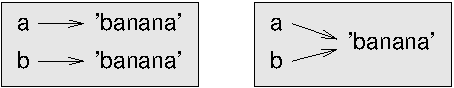
\includegraphics[scale=0.8]{figs/list1.pdf}}
\caption{State diagram.}
\label{fig.list1}
\end{figure}


In one case, {\tt a} and {\tt b} refer to two different objects that
have the same value.  In the second case, they refer to the same
object.
\index{is operator}
\index{operator!is}

一种情况下,{\tt a}和{\tt b}引用两个不同的对象,它们有相同的值。
另一种情况是它们引用相同的对象。

To check whether two variables refer to the same object, you can
use the {\tt is} operator.

为了查看两个变量是否引用同一个对象,你可以使用{\tt is}运算符。

\begin{verbatim}
>>> a = 'banana'
>>> b = 'banana'
>>> a is b
True
\end{verbatim}
%
In this example, Python only created one string object,
and both {\tt a} and {\tt b} refer to it.

此例中,Python生成一个字符串对象,{\tt a}和{\tt b}都引用它。

But when you create two lists, you get two objects:

但是,当你生成两个列表时,你获得两个对象:

\begin{verbatim}
>>> a = [1, 2, 3]
>>> b = [1, 2, 3]
>>> a is b
False
\end{verbatim}
%
So the state diagram looks like Figure~\ref{fig.list2}.
\index{state diagram}
\index{diagram!state}

所以状态图看起来类似图\ref{fig.list2}。

\begin{figure}
\centerline
{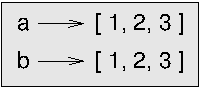
\includegraphics[scale=0.8]{figs/list2.pdf}}
\caption{State diagram.}
\label{fig.list2}
\end{figure}


In this case we would say that the two lists are {\bf equivalent},
because they have the same elements, but not {\bf identical}, because
they are not the same object.  If two objects are identical, they are
also equivalent, but if they are equivalent, they are not necessarily
identical.
\index{equivalence}
\index{identity}

此例中,我们应该说两个列表{\bf 相等(equivalent)},
因为它们具有相同的元素,但不是{\bf 相同(identical)},
因为它们不是相同的对象。
如果两个对象相同,那么它们也是相等的,
但是如果它们相等,它们不一定相同。

Until now, we have been using ``object'' and ``value''
interchangeably, but it is more precise to say that an object has a
value.  If you execute {\tt [1,2,3]}, you get a list
object whose value is a sequence of integers.  If another
list has the same elements, we say it has the same value, but
it is not the same object.
\index{object}
\index{value}

迄今为止,我们一直可互换的使用``对象''和``值'',
但是更精确地说,一个对象有一个值。
如果你执行{\tt [1,2,3]},那么你获得一个列表对象,
其值是一个整数序列。
如果另一个列表有相同的元素,我们说它有相同的值,
但是它不是相同的对象。


\section{Aliasing 别名}
\index{aliasing}
\index{reference!aliasing}

If {\tt a} refers to an object and you assign {\tt b = a},
then both variables refer to the same object:

如果{\tt a}引用一个对象并且你赋值{\tt b=a},
那么两个变量引用相同的对象:

\begin{verbatim}
>>> a = [1, 2, 3]
>>> b = a
>>> b is a
True
\end{verbatim}
%
The state diagram looks like Figure~\ref{fig.list3}.
\index{state diagram}
\index{diagram!state}

状态图类似图~\ref{fig.list3}。

\begin{figure}
\centerline
{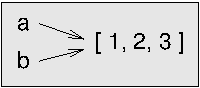
\includegraphics[scale=0.8]{figs/list3.pdf}}
\caption{State diagram.}
\label{fig.list3}
\end{figure}

The association of a variable with an object is called a {\bf
reference}.  In this example, there are two references to the same
object.
\index{reference}

变量和对象之间的关联被称作{\bf 引用(reference)}。
此例中,有两个指向相同对象的引用。

An object with more than one reference has more
than one name, so we say that the object is {\bf aliased}.
\index{mutability}

具有超过一个引用的对象有超过一个的名字,
所以我们说对象被{\bf 别名化(aliased)}了。

If the aliased object is mutable, changes made with one alias affect
the other:

如果别名化的对象是可变的,用一个别名引起的变化影响另一个别名:

\begin{verbatim}
>>> b[0] = 17
>>> print a
[17, 2, 3]
\end{verbatim}
%
Although this behavior can be useful, it is error-prone.  In general,
it is safer to avoid aliasing when you are working with mutable
objects.
\index{immutability}

虽然此行为会是有用的,但是它易于出错。
一般来讲,当你和可变对象一起工作时,避免别名会更安全。

For immutable objects like strings, aliasing is not as much of a
problem.  In this example:

对于想字符串这样的不可变对象,别名不是一个问题。
在此例中:

\begin{verbatim}
a = 'banana'
b = 'banana'
\end{verbatim}
%
It almost never makes a difference whether {\tt a} and {\tt b} refer
to the same string or not.

{\tt a}和{\tt b}是否引用相同的字符串不会引起什么不同。


\section{List arguments 列表实参}
\label{list.arguments}
\index{list!as argument}
\index{argument}
\index{argument!list}
\index{reference}
\index{parameter}

When you pass a list to a function, the function gets a reference
to the list.
If the function modifies a list parameter, the caller sees the change.
For example, \verb"delete_head" removes the first element from a list:

当你向一个函数传递列表时,函数获得指向该列表的引用。
如果函数改变列表形参,那么调用者会看到改变。
例如,\verb"delete_head"从列表中删除第一个元素:

\begin{verbatim}
def delete_head(t):
    del t[0]
\end{verbatim}
%
Here's how it is used:

这是它如何被使用的:

\begin{verbatim}
>>> letters = ['a', 'b', 'c']
>>> delete_head(letters)
>>> print letters
['b', 'c']
\end{verbatim}
%
The parameter {\tt t} and the variable {\tt letters} are
aliases for the same object.  The stack diagram looks like
Figure~\ref{fig.stack5}.
\index{stack diagram}
\index{diagram!stack}

形参{\tt t}和变量{\tt letters}是同一个对象的别名。
栈图如图\ref{fig.stack5}。

\begin{figure}
\centerline
{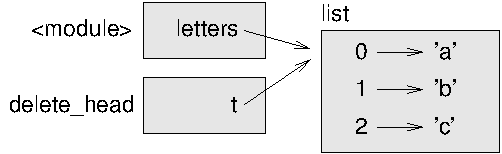
\includegraphics[scale=0.8]{figs/stack5.pdf}}
\caption{Stack diagram.}
\label{fig.stack5}
\end{figure}


Since the list is shared by two frames, I drew
it between them.

既然列表被两个框架共享,我把它画在他们之间。

It is important to distinguish between operations that
modify lists and operations that create new lists.  For
example, the {\tt append} method modifies a list, but the
{\tt +} operator creates a new list:
\index{append method}
\index{method!append}
\index{list!concatenation}
\index{concatenation!list}

区分修改列表和生成新列表的操作非常重要。
例如,{\tt append}方法修改列表,但是{\tt +}运算符生成一个新列表:

\begin{verbatim}
>>> t1 = [1, 2]
>>> t2 = t1.append(3)
>>> print t1
[1, 2, 3]
>>> print t2
None

>>> t3 = t1 + [4]
>>> print t3
[1, 2, 3, 4]
\end{verbatim}

This difference is important when you write functions that
are supposed to modify lists.  For example, this function
{\em does not} delete the head of a list:

当你写一些想要修改列表的函数的时候,此不同非常重要。
例如,此函数并没有删除列表的头:

\begin{verbatim}
def bad_delete_head(t):
    t = t[1:]              # WRONG!
\end{verbatim}

The slice operator creates a new list and the assignment
makes {\tt t} refer to it, but none of that has any effect
on the list that was passed as an argument.
\index{slice operator}
\index{operator!slice}

切片运算符生成一个新的列表,赋值使得{\tt t}引用它,
但是这些对被作为实参传递过来的列表毫无影响。

An alternative is to write a function that creates and
returns a new list.  For
example, {\tt tail} returns all but the first
element of a list:

替代的方法是写一个函数,生成并返回一个新列表。
例如,{\tt tail}返回列表除第一个外的所有元素。

\begin{verbatim}
def tail(t):
    return t[1:]
\end{verbatim}
%
This function leaves the original list unmodified.
Here's how it is used:

此函数不修改原来的列表。
这是如何使用它:

\begin{verbatim}
>>> letters = ['a', 'b', 'c']
>>> rest = tail(letters)
>>> print rest
['b', 'c']
\end{verbatim}



\section{Debugging 调试}
\index{debugging}

Careless use of lists (and other mutable objects)
can lead to long hours of debugging.  Here are some common
pitfalls and ways to avoid them:

不仔细的列表使用(以及其它可变对象)可能导致长时间的调试。
这是一些通常的陷阱以及避免他们的方法:

\begin{enumerate}

\item Don't forget that most list methods modify the argument and
  return {\tt None}.  This is the opposite of the string methods,
  which return a new string and leave the original alone.
  
  不要忘记大多数列表方法修改实参并返回{\tt None}。
  这和字符串方法相反,其返回一个新的字符串并将原始的字符串放在一边。

If you are used to writing string code like this:

如果你想这样写过字符串代码:

\begin{verbatim}
word = word.strip()
\end{verbatim}

It is tempting to write list code like this:

像这样写列表代码也很有诱惑力:

\begin{verbatim}
t = t.sort()           # WRONG!
\end{verbatim}
\index{sort method}
\index{method!sort}

Because {\tt sort} returns {\tt None}, the
next operation you perform with {\tt t} is likely to fail.

因为{\tt sort}返回{\tt None},所以对{\tt t}的进一步运算很可能会失败。

Before using list methods and operators, you should read the
documentation carefully and then test them in interactive mode.  The
methods and operators that lists share with other sequences (like
strings) are documented at
\url{docs.python.org/lib/typesseq.html}.  The
methods and operators that only apply to mutable sequences
are documented at \url{docs.python.org/lib/typesseq-mutable.html}.

在使用列表方法之前,你应该仔细的阅读文档,
然后在交互模式下测试它们。
列表和其它序列(如字符串)共享的方法和运算符的文档位于:
\url{docs.python.org/lib/typesseq.html}。
只能被用于可变序列的方法和运算符的文档在
\url{docs.python.org/lib/typesseq-mutable.html}。


\item Pick an idiom and stick with it.

选择一个习惯并检查下去。

Part of the problem with lists is that there are too many
ways to do things.  For example, to remove an element from
a list, you can use {\tt pop}, {\tt remove}, {\tt del},
or even a slice assignment.

列表的一部分问题是有太多的方法做事情。
例如,为了从列表中删除一个元素,
你可以使用{\tt pop}、{\tt remove}、{\tt del},
甚至一个切片赋值。

To add an element, you can use the {\tt append} method or
the {\tt +} operator.  Assuming that {\tt t} is a list and
{\tt x} is a list element, these are right: 

为了增加一个元素,你可以用{\tt append}方法或者{\tt +}运算符。
假设{\tt t}是一个列表,{\tt x}是一个列表元素,这些都是正确的:

\begin{verbatim}
t.append(x)
t = t + [x]
\end{verbatim}

And these are wrong:

这些是错误的:

\begin{verbatim}
t.append([x])          # WRONG!
t = t.append(x)        # WRONG!
t + [x]                # WRONG!
t = t + x              # WRONG!
\end{verbatim}

Try out each of these examples in interactive mode to make sure
you understand what they do.  Notice that only the last
one causes a runtime error; the other three are legal, but they
do the wrong thing.

在交互模式下测试每个例子,确保你理解他们做了什么。
主意,只有最后一个引起运行时错误,其它三个是合法的,
但是它们做了错误的事情。


\item Make copies to avoid aliasing.
\index{aliasing!copying to avoid}
\index{copy!to avoid aliasing}

用复制,避免别名。

If you want to use a method like {\tt sort} that modifies
the argument, but you need to keep the original list as
well, you can make a copy.

如果你想使用类似{\tt sort}的方法来修改实参,
但是也你需要保留原始列表,那么你可以复制它。

\begin{verbatim}
orig = t[:]
t.sort()
\end{verbatim}

In this example you could also use the built-in function {\tt sorted},
which returns a new, sorted list and leaves the original alone.
But in that case you should avoid using {\tt sorted} as a variable
name!

此例中你也可以使用内建函数{\tt sorted},
其返回一个新的、排好序的列表并将原始列表放在一边。
但是在那个例子中,你应该避免将{\tt sorted}作为变量名使用!

\end{enumerate}



\section{Glossary 术语表}

\begin{description}

\item[list(列表):] A sequence of values.
\index{list}

\item[element(元素):] One of the values in a list (or other sequence),
also called items.
\index{element}

\item[index(索引):] An integer value that indicates an element in a list.
\index{index}

\item[nested list(嵌套的列表):] A list that is an element of another list.
\index{nested list}

\item[list traversal(列表遍历):] The sequential accessing of each element in a list.
\index{list!traversal}

\item[mapping(映射):] A relationship in which each element of one set
corresponds to an element of another set.  For example, a list is
a mapping from indices to elements.
\index{mapping}

\item[accumulator(累加器):] A variable used in a loop to add up or
accumulate a result.
\index{accumulator}

\item[augmented assignment(增量赋值):] A statement that updates the value
of a variable using an operator like \verb"+=".
\index{assignment!augmented}
\index{augmented assignment}
\index{traversal}

\item[reduce(消减):] A processing pattern that traverses a sequence 
and accumulates the elements into a single result.
\index{reduce pattern}
\index{pattern!reduce}

\item[map(映射):] A processing pattern that traverses a sequence and
performs an operation on each element.
\index{map pattern}
\index{pattern!map}

\item[filter(过滤):] A processing pattern that traverses a list and
selects the elements that satisfy some criterion.
\index{filter pattern}
\index{pattern!filter}

\item[object(对象):] Something a variable can refer to.  An object
has a type and a value.
\index{object}

\item[equivalent(相等的):] Having the same value.
\index{equivalent}

\item[identical(相同的):] Being the same object (which implies equivalence).
\index{identical}

\item[reference(引用):] The association between a variable and its value.
\index{reference}

\item[aliasing(别名):] A circumstance where two or more variables refer to the same
object.
\index{aliasing}

\item[delimiter(分隔符):] A character or string used to indicate where a
string should be split.
\index{delimiter}

\end{description}


\section{Exercises}

\begin{exercise}
Write a function called \verb"is_sorted" that takes a list as a
parameter and returns {\tt True} if the list is sorted in ascending
order and {\tt False} otherwise.  You can assume (as a precondition)
that the elements of the list can be compared with the relational
operators {\tt <}, {\tt >}, etc.
\index{precondition}

For example, \verb"is_sorted([1,2,2])" should return {\tt True}
and \verb"is_sorted(['b','a'])" should return {\tt False}.
\end{exercise}


\begin{exercise}
\label{anagram}
\index{anagram}

Two words are anagrams if you can rearrange the letters from one
to spell the other.  Write a function called \verb"is_anagram"
that takes two strings and returns {\tt True} if they are anagrams.
\end{exercise}


\begin{exercise}
\label{duplicate}

The (so-called) Birthday Paradox:

\begin{enumerate}

\item Write a function called \verb"has_duplicates" that takes
a list and returns {\tt True} if there is any element that
appears more than once.  It should not modify the original
list.
\index{birthday paradox}
\index{duplicate}

\item If there are 23 students in your class, what are the chances
that two of you have the same birthday?  You can estimate this
probability by generating random samples of 23 birthdays
and checking for matches.  Hint: you can generate random birthdays
with the {\tt randint} function in the {\tt random} module.
\index{random module}
\index{module!random}
\index{randint function}
\index{function!randint}

\end{enumerate}

You can read about this problem at
\url{http://en.wikipedia.org/wiki/Birthday_paradox}, and you can download my
solution from \url{http://thinkpython.com/code/birthday.py}.

\end{exercise}


\begin{exercise}
\index{duplicate}
\index{uniqueness}

Write a function called \verb"remove_duplicates" that takes
a list and returns a new list with only the unique elements from
the original.  Hint: they don't have to be in the same order.
\end{exercise}


\begin{exercise}
\index{append method}
\index{method append}
\index{list!concatenation}
\index{concatenation!list}

Write a function that reads the file {\tt words.txt} and builds
a list with one element per word.  Write two versions of
this function, one using the {\tt append} method and the
other using the idiom {\tt t = t + [x]}.  Which one takes
longer to run?  Why?

Hint: use the {\tt time} module to measure elapsed time.
Solution: \url{http://thinkpython.com/code/wordlist.py}.
\index{time module}
\index{module!time}

\end{exercise}


\begin{exercise}
\label{wordlist1}
\label{bisection}
\index{membership!bisection search}
\index{bisection search}
\index{search, bisection}
\index{membership!binary search}
\index{binary search}
\index{search, binary}

To check whether a word is in the word list, you could use
the {\tt in} operator, but it would be slow because it searches
through the words in order.

Because the words are in alphabetical order, we can speed things up
with a bisection search (also known as binary search), which is
similar to what you do when you look a word up in the dictionary.  You
start in the middle and check to see whether the word you are looking
for comes before the word in the middle of the list.  If so, then you
search the first half of the list the same way.  Otherwise you search
the second half.

Either way, you cut the remaining search space in half.  If the
word list has 113,809 words, it will take about 17 steps to
find the word or conclude that it's not there.

Write a function called {\tt bisect} that takes a sorted list
and a target value and returns the index of the value
in the list, if it's there, or {\tt None} if it's not.
\index{bisect module}
\index{module!bisect}

Or you could read the documentation of the {\tt bisect} module
and use that!  Solution: \url{http://thinkpython.com/code/inlist.py}.

\end{exercise}

\begin{exercise}
\index{reverse word pair}

Two words are a ``reverse pair'' if each is the reverse of the
other.  Write a program that finds all the reverse pairs in the
word list.  Solution: \url{http://thinkpython.com/code/reverse_pair.py}.

\end{exercise}

\begin{exercise}
\index{interlocking words}

Two words ``interlock'' if taking alternating letters from each forms
a new word.  For example, ``shoe'' and ``cold''
interlock to form ``schooled.''
Solution: \url{http://thinkpython.com/code/interlock.py}.
Credit: This exercise is inspired by an example at \url{http://puzzlers.org}.

\begin{enumerate}

\item Write a program that finds all pairs of words that interlock.
  Hint: don't enumerate all pairs!

\item Can you find any words that are three-way interlocked; that is,
  every third letter forms a word, starting from the first, second or
  third?

\end{enumerate}
\end{exercise}


\chapter{Dictionaries 字典}

\index{dictionary}
\index{dictionary}
\index{type!dict}
\index{key}
\index{key-value pair}
\index{index}
A {\bf dictionary} is like a list, but more general.  In a list,
the indices have to be integers; in a dictionary they can
be (almost) any type.

{\bf 字典(dictionary)}和列表类似,但是更一般。
在列表中,索引必须是整数,在字典中,它们可以是(几乎)任意类型。

You can think of a dictionary as a mapping between a set of indices
(which are called {\bf keys}) and a set of values.  Each key maps to a
value.  The association of a key and a value is called a {\bf
  key-value pair} or sometimes an {\bf item}.
  
你可以将字典看成是索引集合(其被称作{\bf 键(keys)})和值集合直接的映射。
每个键映射到一个值。键和值的关联被称作{\bf 键-值对(key-value pair)}
或者 {\bf (item)}。

As an example, we'll build a dictionary that maps from English
to Spanish words, so the keys and the values are all strings.

作为一个例子,我们将创建一个字典,从英语单词映射到西班牙语单词,
因此键和值都是字符串。

The function {\tt dict} creates a new dictionary with no items.
Because {\tt dict} is the name of a built-in function, you
should avoid using it as a variable name.
\index{dict function}
\index{function!dict}

{\tt dict}函数生成一个新的没有任何项的字典。
因为{\tt dict}是内建函数名,你应该避免将其用于变量名。

\begin{verbatim}
>>> eng2sp = dict()
>>> print eng2sp
{}
\end{verbatim}

The squiggly-brackets, \verb"{}", represent an empty dictionary.
To add items to the dictionary, you can use square brackets:
\index{squiggly bracket}
\index{bracket!squiggly}

花括号\verb"{}"表示一个空字典。为了向字典内增加项,
你可以使用方括号:

\begin{verbatim}
>>> eng2sp['one'] = 'uno'
\end{verbatim}
%
This line creates an item that maps from the key
{\tt 'one'} to the value \verb"'uno'".  If we print the
dictionary again, we see a key-value pair with a colon
between the key and value:

该行生成一个项,从键{\tt 'one'}映射到值\verb"'uno'"。
如果我们再次打印该字典,我们看到一个键-值对,
键和值之间有一个冒号。

\begin{verbatim}
>>> print eng2sp
{'one': 'uno'}
\end{verbatim}
%
This output format is also an input format.  For example,
you can create a new dictionary with three items:

此输出格式也是一个输入格式。
例如,你可以用三个项生成一个新的字典:

\begin{verbatim}
>>> eng2sp = {'one': 'uno', 'two': 'dos', 'three': 'tres'}
\end{verbatim}
%
But if you print {\tt eng2sp}, you might be surprised:

但是,如果你打印{\tt eng2sp},你可能很奇怪:

\begin{verbatim}
>>> print eng2sp
{'one': 'uno', 'three': 'tres', 'two': 'dos'}
\end{verbatim}
%
The order of the key-value pairs is not the same.  In fact, if
you type the same example on your computer, you might get a
different result.  In general, the order of items in
a dictionary is unpredictable.

键-值对的顺序和原来不同。事实上,如果你在你的计算机上键入相同的例子,
你可能获得不同的结果。通常,字典中项的顺序是不可预知的。

But that's not a problem because
the elements of a dictionary are never indexed with integer indices.
Instead, you use the keys to look up the corresponding values:

但这不是个问题,因为字典的元素从不会被用整数索引来索引。
相反,你使用键来查找相应的值:

\begin{verbatim}
>>> print eng2sp['two']
'dos'
\end{verbatim}
%
The key {\tt 'two'} always maps to the value \verb"'dos'" so the order
of the items doesn't matter.

键{\tt 'two'}总是映射到值\verb"'dos'",因此项的顺序没有关系。

If the key isn't in the dictionary, you get an exception:
\index{exception!KeyError}
\index{KeyError}

如果键不在字典中,那么你得到一个异常:

\begin{verbatim}
>>> print eng2sp['four']
KeyError: 'four'
\end{verbatim}
%
The {\tt len} function works on dictionaries; it returns the
number of key-value pairs:
\index{len function}
\index{function!len}

{\tt len}函数对字典起作用,它返回键-值对的数量:

\begin{verbatim}
>>> len(eng2sp)
3
\end{verbatim}
%
The {\tt in} operator works on dictionaries; it tells you whether
something appears as a {\em key} in the dictionary (appearing
as a value is not good enough).
\index{membership!dictionary}
\index{in operator}
\index{operator!in}

{\tt in}运算符对字典起作用,他告诉你是否一些东西在字典中作为键出现
(作为值出现不够好)。

\begin{verbatim}
>>> 'one' in eng2sp
True
>>> 'uno' in eng2sp
False
\end{verbatim}
%
To see whether something appears as a value in a dictionary, you
can use the method {\tt values}, which returns the values as
a list, and then use the {\tt in} operator:
\index{values method}
\index{method!values}

为了看是否一些东西作为值出现,你可以使用{\tt values}方法,
其作为一个列表返回值,然后使用{\tt in}运算符:

\begin{verbatim}
>>> vals = eng2sp.values()
>>> 'uno' in vals
True
\end{verbatim}
%
The {\tt in} operator uses different algorithms for lists and
dictionaries.  For lists, it uses a search algorithm, as in
Section~\ref{find}.  As the list gets longer, the search time gets
longer in direct proportion.  For dictionaries, Python uses an
algorithm called a {\bf hashtable} that has a remarkable property: the
{\tt in} operator takes about the same amount of time no matter how
many items there are in a dictionary.  I won't explain how that's
possible, but you can read more about it at
\url{http://en.wikipedia.org/wiki/Hash_table}.
\index{hashtable}

对于列表和字典,{\tt in}运算符使用不同的算法。
对于列表,它使用如\ref{find}节中的搜索算法。
随着列表的增长,搜索时间成正比增长。
对于字典,Python使用一种叫做{\bf 哈希表(hashtable)}的算法,
其具有非凡的性质:无论字典中有多少项,{\tt in}运算符几乎花费相同的时间。
我不会介绍这怎么可能,但是你可以在\url{http://en.wikipedia.org/wiki/Hash_table}
读到更多关于它的内容。\footnote{译者注:附录\ref{hashtable}介绍了关于哈希表的更多内容。}

\begin{exercise}
\label{wordlist2}
\index{set membership}
\index{membership!set}

Write a function that reads the words in {\tt words.txt} and
stores them as keys in a dictionary.  It doesn't matter what the
values are.  Then you can use the {\tt in} operator
as a fast way to check whether a string is in
the dictionary.

If you did Exercise~\ref{wordlist1}, you can compare the speed
of this implementation with the list {\tt in} operator and the
bisection search.

\end{exercise}


\section{Dictionary as a set of counters 字典作为计数器集合}
\label{histogram}
\index{counter}

Suppose you are given a string and you want to count how many
times each letter appears.  There are several ways you could do it:

假设给你一个字符串,你想计算每个字母出现的次数。
有多种方法可以可以使用:

\begin{enumerate}

\item You could create 26 variables, one for each letter of the
alphabet.  Then you could traverse the string and, for each
character, increment the corresponding counter, probably using
a chained conditional.

你可以生成26个变量,每个对应一个字母表中的字母。
然后你可以遍历字符串,对于每个字符,递增相应的计数器,
可能使用链式条件。

\item You could create a list with 26 elements.  Then you could
convert each character to a number (using the built-in function
{\tt ord}), use the number as an index into the list, and increment
the appropriate counter.

你可以生成具有26个元素的列表。
然后你可以将每个字符传化为一个数字(使用内建函数{\tt ord}),
使用这些数字作为列表的索引,并递增适当的计数器。

\item You could create a dictionary with characters as keys
and counters as the corresponding values.  The first time you
see a character, you would add an item to the dictionary.  After
that you would increment the value of an existing item.

你可以生成一个字典,将字符作为键,计数器作为相应的值。
第一次看到一个字母,你应该向字典中增加一项。
这之后,你应该递增一个已有项的值。

\end{enumerate}

Each of these options performs the same computation, but each
of them implements that computation in a different way.
\index{implementation}

每个选择执行相同的计算,但是它们用不同的方法。

An {\bf implementation} is a way of performing a computation;
some implementations are better than others.  For example,
an advantage of the dictionary implementation is that we don't
have to know ahead of time which letters appear in the string
and we only have to make room for the letters that do appear.

一个{\bf 实现(implementation)}是执行一个计算的方法;
一些实现比另一些好。
例如,字典实现的好处是我们不必事先知道字符串中出现了哪些字母,
我们只需要当这些字母出现时在给它们分配空间。

Here is what the code might look like:

代码可能是这样:

\begin{verbatim}
def histogram(s):
    d = dict()
    for c in s:
        if c not in d:
            d[c] = 1
        else:
            d[c] += 1
    return d
\end{verbatim}
%
The name of the function is {\bf histogram}, which is a statistical
term for a set of counters (or frequencies).
\index{histogram}
\index{frequency}
\index{traversal}

函数名是{\bf 直方图(histogram)},
其是一个统计术语,用于计数器的集合(或者频率)。

The first line of the
function creates an empty dictionary.  The {\tt for} loop traverses
the string.  Each time through the loop, if the character {\tt c} is
not in the dictionary, we create a new item with key {\tt c} and the
initial value 1 (since we have seen this letter once).  If {\tt c} is
already in the dictionary we increment {\tt d[c]}.
\index{histogram}

函数的第一行生成一个字典。{\tt for}循环遍历该字符串。
每次循环,如果字符{\tt c}不在字典中,
我们用键{\tt c}和初始值1生成一个新项
(既然我们已经见过一次该字母了)。
如果{\tt c}已经在字典中了,那么我们递增{\tt d[c]}。

Here's how it works:

这是它如何工作的:

\begin{verbatim}
>>> h = histogram('brontosaurus')
>>> print h
{'a': 1, 'b': 1, 'o': 2, 'n': 1, 's': 2, 'r': 2, 'u': 2, 't': 1}
\end{verbatim}
%
The histogram indicates that the letters {\tt 'a'} and \verb"'b'"
appear once; \verb"'o'" appears twice, and so on.

此直方图表明,字母{\tt 'a'}和\verb"'b'"出现一次;
\verb"'o'"出现两次等等。

\begin{exercise}
\index{get method}
\index{method!get}

Dictionaries have a method called {\tt get} that takes a key
and a default value.  If the key appears in the dictionary,
{\tt get} returns the corresponding value; otherwise it returns
the default value.  For example:

\begin{verbatim}
>>> h = histogram('a')
>>> print h
{'a': 1}
>>> h.get('a', 0)
1
>>> h.get('b', 0)
0
\end{verbatim}
%
Use {\tt get} to write {\tt histogram} more concisely.  You
should be able to eliminate the {\tt if} statement.
\end{exercise}


\section{Looping and dictionaries 循环和字典}
\index{dictionary!looping with}
\index{looping!with dictionaries}
\index{traversal}

If you use a dictionary in a {\tt for} statement, it traverses
the keys of the dictionary.  For example, \verb"print_hist"
prints each key and the corresponding value:

如果你在{\tt for}中使用字典,那么它遍历该字典的键。
例如\verb"print_hist"打印每个键以及相应的值:

\begin{verbatim}
def print_hist(h):
    for c in h:
        print c, h[c]
\end{verbatim}
%
Here's what the output looks like:

输出类似:

\begin{verbatim}
>>> h = histogram('parrot')
>>> print_hist(h)
a 1
p 1
r 2
t 1
o 1
\end{verbatim}
%
Again, the keys are in no particular order.

再一次,键没有什么顺序:

\begin{exercise}
\index{keys method}
\index{method!keys}

Dictionaries have a method called {\tt keys} that returns
the keys of the dictionary, in no particular order, as a list.

Modify \verb"print_hist" to print the keys and their values
in alphabetical order.
\end{exercise}



\section{Reverse lookup 逆向查找}
\label{raise}
\index{dictionary!lookup}
\index{dictionary!reverse lookup}
\index{lookup, dictionary}
\index{reverse lookup, dictionary}

Given a dictionary {\tt d} and a key {\tt k}, it is easy to
find the corresponding value {\tt v = d[k]}.  This operation
is called a {\bf lookup}.

给出一个字典{\tt d}以及一个键{\tt t},很容易找到相应的值{\tt v = d[k]}。
该运算被称作{\bf 查找(lookup)}

But what if you have {\tt v} and you want to find {\tt k}?
You have two problems: first, there might be more than one
key that maps to the value {\tt v}.  Depending on the application,
you might be able to pick one, or you might have to make
a list that contains all of them.  Second, there is no
simple syntax to do a {\bf reverse lookup}; you have to search.

但是,如果你有{\tt v}并且想找到{\tt k}该怎么办呢?
你有两个问题:第一,可能有不止一个的键其映射到值{\tt v}。
依赖于应用,你可能选择一个或者不得不生成一个包含所有键的列表。
第二,没有简单的语法完成{\bf 逆向查找(reverse lookup)};
你必须搜索。

Here is a function that takes a value and returns the first
key that maps to that value:

这是一个函数,接受一个值并返回其映射到该值的第一个键:

\begin{verbatim}
def reverse_lookup(d, v):
    for k in d:
        if d[k] == v:
            return k
    raise ValueError
\end{verbatim}
%
This function is yet another example of the search pattern, but it
uses a feature we haven't seen before, {\tt raise}.  The {\tt raise}
statement causes an exception; in this case it causes a {\tt
  ValueError}, which generally indicates that there is something wrong
with the value of a parameter.
\index{search}
\index{pattern!search}
\index{raise statement}
\index{statement!raise}
\index{exception!ValueError}
\index{ValueError}

该函数是搜索模式的另一个例子,但是它使用了一个我们之前没有见过的特征,{\tt raise}。
{\tt raise}语句引起一个异常;此例中它引起一个{\tt ValueError},
通常其表示形参的值有一些错误。

If we get to the end of the loop, that means {\tt v}
doesn't appear in the dictionary as a value, so we raise an
exception.

我们我们到达循环结尾,这意味着 {\tt v}在字典中不作为值存在,
所以我们触发一个异常。

Here is an example of a successful reverse lookup:

这是一个成功逆向查找的例子:

\begin{verbatim}
>>> h = histogram('parrot')
>>> k = reverse_lookup(h, 2)
>>> print k
r
\end{verbatim}
%
And an unsuccessful one:

和一个不成功的例子:

\begin{verbatim}
>>> k = reverse_lookup(h, 3)
Traceback (most recent call last):
  File "<stdin>", line 1, in ?
  File "<stdin>", line 5, in reverse_lookup
ValueError
\end{verbatim}
%
The result when you raise an exception is the same as when
Python raises one: it prints a traceback and an error message.
\index{traceback}
\index{optional argument}
\index{argument!optional}

当你触发一个异常时,结果和Python触发一个一样:
它打印一个回溯和一个错误信息。

The {\tt raise} statement takes a detailed error message as an
optional argument.  For example:

{\tt raise}语句接受一个详细的错误信息作为可选的实参。
例如:

\begin{verbatim}
>>> raise ValueError, 'value does not appear in the dictionary'
Traceback (most recent call last):
  File "<stdin>", line 1, in ?
ValueError: value does not appear in the dictionary
\end{verbatim}
%
A reverse lookup is much slower than a forward lookup; if you
have to do it often, or if the dictionary gets big, the performance
of your program will suffer.

逆向查找比正向查找慢得多;如果你必须经常做它或者字典很大,
你的程序的性能将变得很差。

\begin{exercise}

Modify \verb"reverse_lookup" so that it builds and returns a list
of {\em all} keys that map to {\tt v}, or an empty list if there
are none.

\end{exercise}


\section{Dictionaries and lists 字典和列表}
\label{invert}

Lists can appear as values in a dictionary.  For example, if you
were given a dictionary that maps from letters to frequencies, you
might want to invert it; that is, create a dictionary that maps
from frequencies to letters.  Since there might be several letters
with the same frequency, each value in the inverted dictionary
should be a list of letters.
\index{invert dictionary}
\index{dictionary!invert}

在字典中,列表可以作为值出现。例如,如果你给你一个从字母映射到频率的字典,
你可能想倒转它;也就是生成一个从频率映射到字母的字典。
既然可能有些字母具有相同的频率,那么在倒转字典中的每个值应该是一个字母的列表。

Here is a function that inverts a dictionary:

这是一个倒转字典的函数:

\begin{verbatim}
def invert_dict(d):
    inverse = dict()
    for key in d:
        val = d[key]
        if val not in inverse:
            inverse[val] = [key]
        else:
            inverse[val].append(key)
    return inverse
\end{verbatim}
%
Each time through the loop, {\tt key} gets a key from {\tt d} and 
{\tt val} gets the corresponding value.  If {\tt val} is not in {\tt inverse},
that means we haven't seen it before, so we create a new item and
initialize it with a {\bf singleton} (a list that contains a
single element).  Otherwise we have seen this value before, so we
append the corresponding key to the list.
\index{singleton}

每次循环,{\tt key}从{\tt d}获得一个键和相应的值{\tt val}。
如果{\tt val}不在{\tt inverse}中,这意味着我们之前没有见过它,
因此我们生成一个新项并用一个{\bf 单元素集合(singleton)}(包括唯一元素的列表)
初始化它。

Here is an example:

这是一个例子:

\begin{verbatim}
>>> hist = histogram('parrot')
>>> print hist
{'a': 1, 'p': 1, 'r': 2, 't': 1, 'o': 1}
>>> inverse = invert_dict(hist)
>>> print inverse
{1: ['a', 'p', 't', 'o'], 2: ['r']}
\end{verbatim}

\begin{figure}
\centerline
{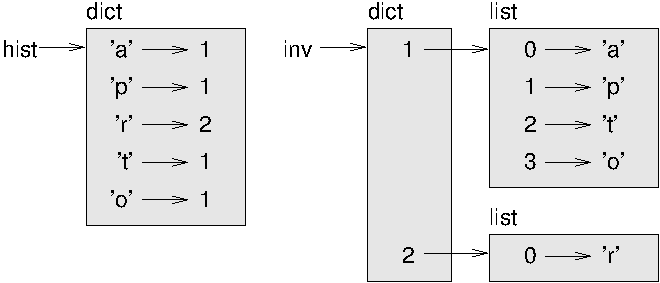
\includegraphics[scale=0.8]{figs/dict1.pdf}}
\caption{State diagram.}
\label{fig.dict1}
\end{figure}

Figure~\ref{fig.dict1} is a state diagram showing {\tt hist} and {\tt inverse}.
A dictionary is represented as a box with the type {\tt dict} above it
and the key-value pairs inside.  If the values are integers, floats or
strings, I usually draw them inside the box, but I usually draw lists
outside the box, just to keep the diagram simple.
\index{state diagram}
\index{diagram!state}

图\ref{fig.dict1}是一个状态图,显示{\tt hist}和{\tt inverse}。
一个字典被表示为一个盒子,类型类型{\tt dict}在上面,键-值对在里面。
如果值是整数、浮点数或者字符串,那么我通常把他们画在盒子里,
但是我通常将列表画在盒子外,仅仅是为了使图简洁。

Lists can be values in a dictionary, as this example shows, but they
cannot be keys.  Here's what happens if you try:
\index{TypeError}
\index{exception!TypeError}

字典中,列表可以是值,如此例所示,但是它们不能是键。
如果你试图这样做,这是会发生什么:

\begin{verbatim}
>>> t = [1, 2, 3]
>>> d = dict()
>>> d[t] = 'oops'
Traceback (most recent call last):
  File "<stdin>", line 1, in ?
TypeError: list objects are unhashable
\end{verbatim}
%
I mentioned earlier that a dictionary is implemented using
a hashtable and that means that the keys have to be {\bf hashable}.
\index{hash function}
\index{hashable}

我之前提过,字典使用哈希表实现,这意味着键必须是{\bf 可哈希的(hashable)}。

A {\bf hash} is a function that takes a value (of any kind)
and returns an integer.  Dictionaries use these integers,
called hash values, to store and look up key-value pairs.
\index{immutability}

{\bf 哈希(hash)}是一个函数,接受一个值(任何类型)并返回一个整数。
字典使用这些整数,被称作哈希值,来存储和查找键-值对。

This system works fine if the keys are immutable.  But if the
keys are mutable, like lists, bad things happen.  For example,
when you create a key-value pair, Python hashes the key and 
stores it in the corresponding location.  If you modify the
key and then hash it again, it would go to a different location.
In that case you might have two entries for the same key,
or you might not be able to find a key.  Either way, the
dictionary wouldn't work correctly.

如果键是不可变的,此系统工作的很好。
但是如果键是可变的,如列表,那么坏事情发生了。
例如,当你生成一个键-值对的时候,Python哈希键并将其存储在相应的位置。
如果你改变键然后再次哈希它,它将到另一个位置。
在那种情况下,对于相同的键,你可能有两个入口,
或者你可能不能找到一个键。
无论如何,字典都不会正确的工作。

That's why the keys have to be hashable, and why mutable types like
lists aren't.  The simplest way to get around this limitation is to
use tuples, which we will see in the next chapter.

这是为什么键必须是可哈希的,以及为什么可变类型,如列表就不是。
绕过这种限制最简单的方法是使用元组,
我们将在下一章中介绍。

Since dictionaries are mutable, they can't be used as keys,
but they {\em can} be used as values.

既然字典是可变的,它们不能被用作键,
但是它们可以被用作值。

\begin{exercise}
Read the documentation of the dictionary method {\tt setdefault}
and use it to write a more concise version of \verb"invert_dict".
Solution: \url{http://thinkpython.com/code/invert_dict.py}.
\index{setdefault method}
\index{method!setdefault}

\end{exercise}


\section{Memos 备忘录}

If you played with the {\tt fibonacci} function from
Section~\ref{one.more.example}, you might have noticed that the bigger
the argument you provide, the longer the function takes to run.
Furthermore, the run time increases very quickly.
\index{fibonacci function}
\index{function!fibonacci}

如果你调用过\ref{one.more.example}节的{\tt fibonacci}函数,
你可能注意到你提供越大的实参,函数运行的时间越长。
更进一步地,运行时间增长的非常快。

To understand why, consider Figure~\ref{fig.fibonacci}, which shows
the {\bf call graph} for {\tt fibonacci} with {\tt n=4}:

为了理解原因,考虑图\ref{fig.fibonacci},其展示了{\tt n=4}时,
{\tt fibonacci} 的{\bf 调用图(call graph)}。

\begin{figure}
\centerline
{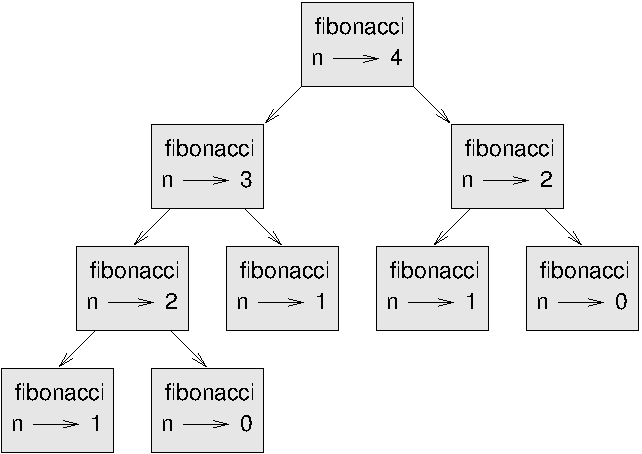
\includegraphics[scale=0.7]{figs/fibonacci.pdf}}
\caption{Call graph.}
\label{fig.fibonacci}
\end{figure}

A call graph shows a set of function frames, with lines connecting each
frame to the frames of the functions it calls.  At the top of the
graph, {\tt fibonacci} with {\tt n=4} calls {\tt fibonacci} with {\tt
n=3} and {\tt n=2}.  In turn, {\tt fibonacci} with {\tt n=3} calls
{\tt fibonacci} with {\tt n=2} and {\tt n=1}.  And so on.
\index{function frame}
\index{frame}
\index{call graph}

调用图显示了函数框架的集合,每个框架到其调用函数的框架用线相连。
在图的顶端,{\tt n=4}的{\tt fibonacci}调用{\tt n=3}和{\tt n=2}的{\tt fibonacci}。
接着,{\tt n=3}的{\tt fibonacci}调用{\tt n=2}和{\tt n=1}的{\tt fibonacci},等等。

Count how many times {\tt fibonacci(0)} and {\tt fibonacci(1)} are
called.  This is an inefficient solution to the problem, and it gets
worse as the argument gets bigger.
\index{memo}

计算{\tt fibonacci(0)}和{\tt fibonacci(1)}被调用多少次。
对该问题,这不是一个有效的解,并且随着实参的变大会变得更糟。

One solution is to keep track of values that have already been
computed by storing them in a dictionary.  A previously computed value
that is stored for later use is called a {\bf memo}.  Here is an
implementation of {\tt fibonacci} using memos:

一个解决办法是保存已经计算过的值,将它们存在一个字典中。
之前计算过的值,其被存储以便今后使用,被称作{\bf 备忘录(memo)}。
这是使用备忘录的{\tt fibonacci}的实现:

\begin{verbatim}
known = {0:0, 1:1}

def fibonacci(n):
    if n in known:
        return known[n]

    res = fibonacci(n-1) + fibonacci(n-2)
    known[n] = res
    return res
\end{verbatim}
%
{\tt known} is a dictionary that keeps track of the Fibonacci
numbers we already know.  It starts with
two items: 0 maps to 0 and 1 maps to 1.

{\tt known}是一个字典,其记录我们已经知道的斐波那契数。
它从两项开始:0映射到0,1映射到1。

Whenever {\tt fibonacci} is called, it checks {\tt known}.
If the result is already there, it can return
immediately.  Otherwise it has to 
compute the new value, add it to the dictionary, and return it.

当{\tt fibonacci}被调用时,它检查{\tt known}。
如果结果已经在那儿了,则立即返回。
否则,它不得不计算新的值,将其加入字典,并返回它。

\begin{exercise}

Run this version of {\tt fibonacci} and the original with
a range of parameters and compare their run times.

\end{exercise}

\begin{exercise}

Memoize the Ackermann function from Exercise~\ref{ackermann} and see if
memoization makes it possible to evaluate the function with bigger
arguments.  Hint: no.

回忆习题~\ref{ackermann}中的Ackermann函数,看看使用备忘录能否使得此函数能计算更大的输入参数。
提示:不能

Solution: \url{http://thinkpython.com/code/ackermann_memo.py}.
\index{Ackermann function}
\index{function!ack}

\end{exercise}


\section{Global variables 全局变量}
\index{global variable}
\index{variable!global}

In the previous example, {\tt known} is created outside the function,
so it belongs to the special frame called \verb"__main__".
Variables in \verb"__main__" are sometimes called {\bf global}
because they can be accessed from any function.  Unlike local
variables, which disappear when their function ends, global variables
persist from one function call to the next.
\index{flag}

在前面的例子中,{\tt known}在函数的外面被生成,
因此它属于特殊的被称作\verb"__main__"的框架。
在\verb"__main__"中的变量有时被称作{\bf 全局的(global)},
因为它们可以从任意函数访问。
和函数结束时它们就会消失的局部变量不同,
全局变量从一个函数调用到另一个调用一直都存在。

It is common to use global variables for {\bf flags}; that is, 
boolean variables that indicate (``flag'') whether a condition
is true.  For example, some programs use
a flag named {\tt verbose} to control the level of detail in the
output:

经常使用全局变量作为{\bf 标记(flags)};
也就是指示(标记)一个条件是否为真的布尔变量。
例如,一些程序使用一个被称作{\tt verbose}的标记来控制
输出中细节的等级:

\begin{verbatim}
verbose = True

def example1():
    if verbose:
        print 'Running example1'
\end{verbatim}
%
If you try to reassign a global variable, you might be surprised.
The following example is supposed to keep track of whether the
function has been called:
\index{multiple assignment}
\index{assignment!multiple}

如果你试图重新对全局变量赋值,你可能会惊讶。
下面的例子本应该能够记录是否该函数已经被调用过了:

\begin{verbatim}
been_called = False

def example2():
    been_called = True         # WRONG
\end{verbatim}
%
But if you run it you will see that the value of \verb"been_called"
doesn't change.  The problem is that {\tt example2} creates a new local
variable named \verb"been_called".  The local variable goes away when
the function ends, and has no effect on the global variable.
\index{global statement}
\index{statement!global}
\index{declaration}

但是如果你运行它,你将发现\verb"been_called"的值没有改变。
问题在于{\tt example2}生成一个新的被称作\verb"been_called"的局部变量。
当函数结束的时候,该局部变量也消失了,并且对全局变量没有影响。

To reassign a global variable inside a function you have to
{\bf declare} the global variable before you use it:

为了在一个函数内部重新对全局变量赋值,
你必须在使用它之前,{\bf 声明(declare)}该全局变量:

\begin{verbatim}
been_called = False

def example2():
    global been_called 
    been_called = True
\end{verbatim}
%
The {\tt global} statement tells the interpreter
something like, ``In this function, when I say \verb"been_called", I
mean the global variable; don't create a local one.''
\index{update!global variable}
\index{global variable!update}

{\tt global}语句告诉解释器诸如此类的事情,
``在此函数中,当我说\verb"been_called"时,我的意思是全局变量;
不要生成局部变量''。

Here's an example that tries to update a global variable:

这是一个试图更新全局变量的例子:

\begin{verbatim}
count = 0

def example3():
    count = count + 1          # WRONG
\end{verbatim}
%
If you run it you get:
\index{UnboundLocalError}
\index{exception!UnboundLocalError}

如果你运行它,你得到:

\begin{verbatim}
UnboundLocalError: local variable 'count' referenced before assignment
\end{verbatim}
%
Python assumes that {\tt count} is local, which means
that you are reading it before writing it.  The solution, again,
is to declare {\tt count} global.
\index{counter}

Python假设{\tt count}是局部的,这意味着你在写它之前,正在读它。
再次,解决方案是声明{\tt count}是全局的。

\begin{verbatim}
def example3():
    global count
    count += 1
\end{verbatim}
%
If the global value is mutable, you can modify it without
declaring it:
\index{mutability}

如果全局值是可变的,你可以修改它,而不用声明:

\begin{verbatim}
known = {0:0, 1:1}

def example4():
    known[2] = 1
\end{verbatim}
%
So you can add, remove and replace elements of a global list or
dictionary, but if you want to reassign the variable, you
have to declare it:

因此你可以增加、删除和替代全局列表或者字典的元素,
但是如果你想对变量重新赋值,你必须声明它:

\begin{verbatim}
def example5():
    global known
    known = dict()
\end{verbatim}
%

\section{Long integers 长整数}
\index{long integer}
\index{integer!long}
\index{type!long}

If you compute {\tt fibonacci(50)}, you get:

如果你计算{\tt fibonacci(50)},你会得到:

\begin{verbatim}
>>> fibonacci(50)
12586269025L
\end{verbatim}
%
The {\tt L} at the end indicates that the result is a long
integer, or type {\tt long}.  In Python 3, {\tt long} is gone; all integers,
even really big ones, are type {\tt int}.
\index{Python 3}

结尾的{\tt L}表明结果是一个长整数,或者说{\tt long}类型。
在Python3中, {\tt long}不存在了;所有的整数,
即使非常大的,也是 {\tt int}类型。

Values with type {\tt int} have a limited range;
long integers can be arbitrarily big, but as they get bigger
they consume more space and time.

{\tt int}类型的值有一个有限的取值范围;
长整数可以任意大,但是随着它们变大,
它们消耗更多的空间和时间。

The mathematical operators work on long integers, and the functions
in the {\tt math} module, too, so in general any code that
works with {\tt int} will also work with {\tt long}.

数学运算可用于长整数并且{\tt math}模块中的函数也可以,
因此一般来讲,任何能用于{\tt int}的代码也能用于 {\tt long}。

Any time the result of a computation is too big to be represented with
an integer, Python converts the result as a long integer:

任何时候,一个太大以至于不能用整数表示的计算结果,
Python会将该结果转化为一个长整数:

\begin{verbatim}
>>> 1000 * 1000
1000000
>>> 100000 * 100000
10000000000L
\end{verbatim}
%
In the first case the result has type {\tt int}; in the
second case it is {\tt long}.

第一个例子中,结果是{\tt int}类型;
第二个例子中,它是{\tt long}。

\begin{exercise}
\index{encryption}
\index{RSA algorithm}
\index{algorithm!RSA}

Exponentiation of large integers is the basis of common
algorithms for public-key encryption.  Read the Wikipedia
page on the RSA algorithm (\url{http://en.wikipedia.org/wiki/RSA})
and write functions to encode and decode messages.

大整数的指数运算是常见公钥加密算法的基础。阅读维基百科RSA算法的页面
(\url{http://en.wikipedia.org/wiki/RSA})并编写加密与解密信息的函数。

% TODO: solution for this one!

\end{exercise}


\section{Debugging 调试}
\index{debugging}

As you work with bigger datasets it can become unwieldy to
debug by printing and checking data by hand.  Here are some
suggestions for debugging large datasets:

当你操作较大的数据集时,通过打印并手工检查数据来调试很不方便。
这是对于调试大数据集合的一些建议:

\begin{description}

\item[Scale down the input:] If possible, reduce the size of the
dataset.  For example if the program reads a text file, start with
just the first 10 lines, or with the smallest example you can find.
You can either edit the files themselves, or (better) modify the
program so it reads only the first {\tt n} lines.

[缩小输入:]如果可能,减小数据集合的大小。
例如,如果程序读取一个文本文件,只以前10行开始,
或者用一个你能找到的小的例子开始。
你或者可以编辑文件,或者(更好)修改程序让它只读取前{\tt n}行。

If there is an error, you can reduce {\tt n} to the smallest
value that manifests the error, and then increase it gradually
as you find and correct errors.

如果有错误,你可以减小{\tt n}到出现错误的最小的值,
然后逐渐增加它,随着你发现错误并改正错误。

\item[Check summaries and types:] Instead of printing and checking the
entire dataset, consider printing summaries of the data: for example,
the number of items in a dictionary or the total of a list of numbers.

[检查摘要和类型:]不用打印并检查全部数据集合,而是考虑打印数据的摘要:
例如字典中项的数目或者数字列表的总和。

A common cause of runtime errors is a value that is not the right
type.  For debugging this kind of error, it is often enough to print
the type of a value.

通常的运行时错误原因是一个值的类型不正确。
为了调试此类错误,打印值的类型通常就足够了。

\item[Write self-checks:]  Sometimes you can write code to check
for errors automatically.  For example, if you are computing the
average of a list of numbers, you could check that the result is
not greater than the largest element in the list or less than
the smallest.  This is called a ``sanity check'' because it detects
results that are ``insane.''
\index{sanity check}
\index{consistency check}

[写自检:]有时你可以写代码来自动检查错误。
例如,如果你正在计算数字列表的平均数,
你可以检查其结果不用大于列表中最大的元素或者不小于最小的。
这被称作``合理性检查'',因为它探测出``不合理的''结果。

Another kind of check compares the results of two different
computations to see if they are consistent.  This is called a
``consistency check.''

另一类检查比较两个不同计算的结果来看一下它们是否一致。
这被称作``一致性检查''。

\item[Pretty print the output:] Formatting debugging output
can make it easier to spot an error.  We saw an example in
Section~\ref{factdebug}.  The {\tt pprint} module provides
a {\tt pprint} function that displays built-in types in
a more human-readable format.
\index{pretty print}
\index{pprint module}
\index{module!pprint}

[美化打印输出:]格式化调试输出能够更容易定位一个错误。
\ref{factdebug}节中我们看到一个例子。
{\tt pprint}模块提供了一个{\tt pprint}函数,
其以更可读的格式显示内建类型。

\end{description}

Again, time you spend building scaffolding can reduce
the time you spend debugging.
\index{scaffolding}

再一次,你花在建立脚手架上的时间能减少你花在调试上的时间。

\section{Glossary 术语表}

\begin{description}

\item[dictionary(字典):] A mapping from a set of keys to their
corresponding values.
\index{dictionary}

\item[key-value pair(键-值对):] The representation of the mapping from
a key to a value.
\index{key-value pair}

\item[item(项):] Another name for a key-value pair.
\index{item!dictionary}

\item[key(键):] An object that appears in a dictionary as the
first part of a key-value pair.
\index{key}

\item[value(值):] An object that appears in a dictionary as the
second part of a key-value pair.  This is more specific than
our previous use of the word ``value.''
\index{value}

\item[implementation(实现):] A way of performing a computation.
\index{implementation}

\item[hashtable(哈希表):] The algorithm used to implement Python
dictionaries.
\index{hashtable}

\item[hash function(哈希函数):] A function used by a hashtable to compute the
location for a key.
\index{hash function}

\item[hashable(可哈希的):] A type that has a hash function.  Immutable
types like integers,
floats and strings are hashable; mutable types like lists and
dictionaries are not.
\index{hashable}

\item[lookup(查找):] A dictionary operation that takes a key and finds
the corresponding value.
\index{lookup}

\item[reverse lookup(逆向查找):] A dictionary operation that takes a value and finds
one or more keys that map to it.
\index{reverse lookup, dictionary}

\item[singleton(单元素集合):] A list (or other sequence) with a single element.
\index{singleton}

\item[call graph(调用图):] A diagram that shows every frame created during
the execution of a program, with an arrow from each caller to
each callee. 
\index{call graph}
\index{diagram!call graph}

\item[histogram(直方图):] A set of counters.
\index{histogram}

\item[memo(备忘录):] A computed value stored to avoid unnecessary future 
computation.
\index{memo}

\item[global variable(全局变量):]  A variable defined outside a function.  Global
variables can be accessed from any function.
\index{global variable}

\item[flag(标记):] A boolean variable used to indicate whether a condition
is true.
\index{flag}

\item[declaration(声明):] A statement like {\tt global} that tells the
interpreter something about a variable.
\index{declaration}

\end{description}

\section{Exercises}

\begin{exercise}
\index{duplicate}

If you did Exercise~\ref{duplicate}, you already have
a function named \verb"has_duplicates" that takes a list
as a parameter and returns {\tt True} if there is any object
that appears more than once in the list.

Use a dictionary to write a faster, simpler version of
\verb"has_duplicates". 
Solution: \url{http://thinkpython.com/code/has_duplicates.py}.

\end{exercise}


\begin{exercise}
\label{exrotatepairs}
\index{letter rotation}
\index{rotation!letters}

Two words are ``rotate pairs'' if you can rotate one of them
and get the other (see \verb"rotate_word" in Exercise~\ref{exrotate}).

Write a program that reads a wordlist and finds all the rotate
pairs.  Solution: \url{http://thinkpython.com/code/rotate_pairs.py}.

\end{exercise}


\begin{exercise}
\index{Car Talk}
\index{Puzzler}

Here's another Puzzler from {\em Car
Talk} (\url{http://www.cartalk.com/content/puzzler/transcripts/200717}):

\begin{quote}
This was sent in by a fellow named Dan O'Leary. He came upon a common
one-syllable, five-letter word recently that has the following unique
property. When you remove the first letter, the remaining letters form
a homophone of the original word, that is a word that sounds exactly
the same. Replace the first letter, that is, put it back and remove
the second letter and the result is yet another homophone of the
original word. And the question is, what's the word?

Now I'm going to give you an example that doesn't work. Let's look at
the five-letter word, `wrack.' W-R-A-C-K, you know like to `wrack with
pain.' If I remove the first letter, I am left with a four-letter
word, 'R-A-C-K.' As in, `Holy cow, did you see the rack on that buck!
It must have been a nine-pointer!' It's a perfect homophone. If you
put the `w' back, and remove the `r,' instead, you're left with the
word, `wack,' which is a real word, it's just not a homophone of the
other two words.

But there is, however, at least one word that Dan and we know of,
which will yield two homophones if you remove either of the first two
letters to make two, new four-letter words. The question is, what's
the word?
\end{quote}
\index{homophone}
\index{reducible word}
\index{word, reducible}

You can use the dictionary from Exercise~\ref{wordlist2} to check
whether a string is in the word list.

To check whether two words are homophones, you can use the CMU
Pronouncing Dictionary.  You can download it from
\url{http://www.speech.cs.cmu.edu/cgi-bin/cmudict} or from
\url{http://thinkpython.com/code/c06d} and you can also download
\url{http://thinkpython.com/code/pronounce.py}, which provides a function
named \verb"read_dictionary" that reads the pronouncing dictionary and
returns a Python dictionary that maps from each word to a string that
describes its primary pronunciation.

Write a program that lists all the words that solve the Puzzler.
Solution: \url{http://thinkpython.com/code/homophone.py}.

\end{exercise}



\chapter{Tuples 元组}
\label{tuplechap}

\section{Tuples are immutable 元组是不可变的}
\index{tuple}
\index{type!tuple}
\index{sequence}

A tuple is a sequence of values.  The values can be any type, and
they are indexed by integers, so in that respect tuples are a lot
like lists.  The important difference is that tuples are immutable.
\index{mutability}
\index{immutability}

元组是一个值的序列。值可以是任意类型,它们以整数索引,
所以从这方面讲元组更像列表。
重要的不同是元组是不可变的。

Syntactically, a tuple is a comma-separated list of values:

语法上,元组是以逗号分割的值的列表:

\begin{verbatim}
>>> t = 'a', 'b', 'c', 'd', 'e'
\end{verbatim}
%
Although it is not necessary, it is common to enclose tuples in
parentheses:
\index{parentheses!tuples in}

虽然并非必须,元组通常用括号括起来:

\begin{verbatim}
>>> t = ('a', 'b', 'c', 'd', 'e')
\end{verbatim}
%
To create a tuple with a single element, you have to include a final
comma:
\index{singleton}
\index{tuple!singleton}

为了用一个单独的元素生成一个元组,
你必须包括最后的逗号:

\begin{verbatim}
>>> t1 = 'a',
>>> type(t1)
<type 'tuple'>
\end{verbatim}
%
A value in parentheses is not a tuple:

括号中的一个值不是元组:

\begin{verbatim}
>>> t2 = ('a')
>>> type(t2)
<type 'str'>
\end{verbatim}
%
Another way to create a tuple is the built-in function {\tt tuple}.
With no argument, it creates an empty tuple:
\index{tuple function}
\index{function!tuple}

生成元组的另一种方法是内建函数{\tt tuple}。
没有实参的话,它生成一个空元组:

\begin{verbatim}
>>> t = tuple()
>>> print t
()
\end{verbatim}
%
If the argument is a sequence (string, list or tuple), the result
is a tuple with the elements of the sequence:

如果实参是一个序列(字符串、列表或元组),
返回值是一个以该序列元组组成的元组。

\begin{verbatim}
>>> t = tuple('lupins')
>>> print t
('l', 'u', 'p', 'i', 'n', 's')
\end{verbatim}
%
Because {\tt tuple} is the name of a built-in function, you should
avoid using it as a variable name.

因为{\tt tuple}是内建函数名,所以你应该避免使用它作为变量名。

Most list operators also work on tuples.  The bracket operator
indexes an element:
\index{bracket operator}
\index{operator!bracket}

大多数列表运算同样适用于元组。括号操作索引一个元素:

\begin{verbatim}
>>> t = ('a', 'b', 'c', 'd', 'e')
>>> print t[0]
'a'
\end{verbatim}
%
And the slice operator selects a range of elements.
\index{slice operator}
\index{operator!slice}
\index{tuple!slice}
\index{slice!tuple}

切片运算符选择一个范围的元素。

\begin{verbatim}
>>> print t[1:3]
('b', 'c')
\end{verbatim}
%
But if you try to modify one of the elements of the tuple, you get
an error:
\index{exception!TypeError}
\index{TypeError}
\index{item assignment}
\index{assignment!item}

但是,如果你试图修改一个元组的元素,你会获得一个错误:

\begin{verbatim}
>>> t[0] = 'A'
TypeError: object doesn't support item assignment
\end{verbatim}
%
You can't modify the elements of a tuple, but you can replace
one tuple with another:

你不能改变元组的元素,但是你可以用一个元组替换另一个:

\begin{verbatim}
>>> t = ('A',) + t[1:]
>>> print t
('A', 'b', 'c', 'd', 'e')
\end{verbatim}
%

\section{Tuple assignment 元组赋值}
\label{tuple.assignment}
\index{tuple!assignment}
\index{assignment!tuple}
\index{swap pattern}
\index{pattern!swap}

It is often useful to swap the values of two variables.
With conventional assignments, you have to use a temporary
variable.  For example, to swap {\tt a} and {\tt b}:

交换两个变量的值通常很有用。
用传统的赋值方法,你必须使用一个临时变量。
例如,为了交换{\tt a}和{\tt b}:

\begin{verbatim}
>>> temp = a
>>> a = b
>>> b = temp
\end{verbatim}
%
This solution is cumbersome; {\bf tuple assignment} is more elegant:

这个解决方案很麻烦;{\bf 元组赋值(tuple assignment)}更优雅:

\begin{verbatim}
>>> a, b = b, a
\end{verbatim}
%
The left side is a tuple of variables; the right side is a tuple of
expressions.  Each value is assigned to its respective variable.  
All the expressions on the right side are evaluated before any
of the assignments.

左侧是一个变量的元组;右侧是表达式的元组。
每个值被赋给它的各自的变量。
右侧的所有表达式在赋值之前被计算。

The number of variables on the left and the number of
values on the right have to be the same:
\index{exception!ValueError}
\index{ValueError}

左侧变量的数目和右侧变量的数目必须相同:

\begin{verbatim}
>>> a, b = 1, 2, 3
ValueError: too many values to unpack
\end{verbatim}
%
More generally, the right side can be any kind of sequence
(string, list or tuple).  For example, to split an email address
into a user name and a domain, you could write:
\index{split method}
\index{method!split}
\index{email address}

更一般地,右侧可以是任意类型的序列(字符串、列表或者元组)。
例如,为了将一个电子邮件地址分割成用户名和域名,
你可以写:

\begin{verbatim}
>>> addr = 'monty@python.org'
>>> uname, domain = addr.split('@')
\end{verbatim}
%
The return value from {\tt split} is a list with two elements;
the first element is assigned to {\tt uname}, the second to
{\tt domain}.

{\tt split}的返回值是一个具有两个元素的列表;
第一个元素被赋给{\tt uname},第二个赋给{\tt domain}。

\begin{verbatim}
>>> print uname
monty
>>> print domain
python.org
\end{verbatim}
%

\section{Tuples as return values 元组作为返回值}
\index{tuple}
\index{value!tuple}
\index{return value!tuple}
\index{function, tuple as return value}

Strictly speaking, a function can only return one value, but
if the value is a tuple, the effect is the same as returning
multiple values.  For example, if you want to divide two integers
and compute the quotient and remainder, it is inefficient to
compute {\tt x/y} and then {\tt x\%y}.  It is better to compute
them both at the same time.
\index{divmod}

严格来讲,一个函数只能返回一个值,但是如果值是一个元组,
则会起到返回多个值的效果。
例如,如果你想除两个整数并计算商和余数,
则先计算{\tt x/y}然后在计算{\tt x\%y}是低效的。
最好同时计算它们俩。

The built-in function {\tt divmod} takes two arguments and
returns a tuple of two values, the quotient and remainder.
You can store the result as a tuple:

内建函数{\tt divmod}接受两个实参并返回两个值的元组,商和余数。
你可以将返回值存为元组:

\begin{verbatim}
>>> t = divmod(7, 3)
>>> print t
(2, 1)
\end{verbatim}
%
Or use tuple assignment to store the elements separately:
\index{tuple assignment}
\index{assignment!tuple}

或者使用元组赋值分别存储元素:

\begin{verbatim}
>>> quot, rem = divmod(7, 3)
>>> print quot
2
>>> print rem
1
\end{verbatim}
%
Here is an example of a function that returns a tuple:

这是一个返回元组的函数的例子:

\begin{verbatim}
def min_max(t):
    return min(t), max(t)
\end{verbatim}
%
{\tt max} and {\tt min} are built-in functions that find
the largest and smallest elements of a sequence.  \verb"min_max"
computes both and returns a tuple of two values.
\index{max function}
\index{function!max}
\index{min function}
\index{function!min}

{\tt max}和{\tt min}是内建函数,其发现一个序列的最大和最小的元素。
\verb"min_max"计算这两个值,并返回一个两个值的元组。


\section{Variable-length argument tuples 变长实参元组}
\index{variable-length argument tuple}
\index{argument!variable-length tuple}
\index{gather}
\index{parameter!gather}
\index{argument!gather}

Functions can take a variable number of arguments.  A parameter
name that begins with {\tt *} {\bf gathers} arguments into
a tuple.  For example, {\tt printall}
takes any number of arguments and prints them:

函数可以接受一个可变数量的实参。
一个以{\tt *}开始的形参名{\bf 汇集(gathers)}实参到一个元组中。
例如,{\tt printall}接受任意数量的实参并打印它们:

\begin{verbatim}
def printall(*args):
    print args
\end{verbatim}
%
The gather parameter can have any name you like, but {\tt args} is
conventional.  Here's how the function works:

汇集的形参可以是任何你喜欢的名字,但是习惯上用{\tt args}。
这是函数如何工作的:

\begin{verbatim}
>>> printall(1, 2.0, '3')
(1, 2.0, '3')
\end{verbatim}
%
The complement of gather is {\bf scatter}.  If you have a
sequence of values and you want to pass it to a function
as multiple arguments, you can use the {\tt *} operator.
For example, {\tt divmod} takes exactly two arguments; it
doesn't work with a tuple:

汇集的补是{\bf 分散(scatter)}。如果你有一序列值,
你想将其作为多个实参传递给一个函数,你可以使用{\tt *}运算符。
例如,{\tt divmod}只接受两个实参;不可以用元组:

% removing this because we haven't seen optional parameters yet
%You can combine the gather operator with required and positional
%arguments:

%%\begin{verbatim}
%def pointless(required, optional=0, *args):
%    print required, optional, args
%\end{verbatim}
%\afterverb
%
%Run this function with 1, 2, 3 and 4 or more arguments and
%make sure you understand what it does.
\index{scatter}
\index{argument scatter}
\index{TypeError}
\index{exception!TypeError}

\begin{verbatim}
>>> t = (7, 3)
>>> divmod(t)
TypeError: divmod expected 2 arguments, got 1
\end{verbatim}
%
But if you scatter the tuple, it works:

但是如果你分散该元组,是可以的:

\begin{verbatim}
>>> divmod(*t)
(2, 1)
\end{verbatim}
%
\begin{exercise}

Many of the built-in functions use
variable-length argument tuples.  For example, {\tt max}
and {\tt min} can take any number of arguments:
\index{max function}
\index{function!max}
\index{min function}
\index{function!min}

\begin{verbatim}
>>> max(1,2,3)
3
\end{verbatim}
%
But {\tt sum} does not.
\index{sum function}
\index{function!sum}

\begin{verbatim}
>>> sum(1,2,3)
TypeError: sum expected at most 2 arguments, got 3
\end{verbatim}
%
Write a function called {\tt sumall} that takes any number
of arguments and returns their sum.

\end{exercise}


\section{Lists and tuples 列表和元组}
\index{zip function}
\index{function!zip}

{\tt zip} is a built-in function that takes two or more sequences and
``zips'' them into a list of tuples where each tuple contains one
element from each sequence.  In Python 3, {\tt zip} returns an iterator
of tuples, but for most purposes, an iterator behaves like a list.
\index{Python 3}

{\tt zip}是一个内建函数,其接受两个或者更多的序列并把它们``zip''到一个元组列表中,
其中每个元组包括来自每个序列的一个元素。
在Python 3中,{\tt zip}返回一个元组的迭代器,
但是对于大多数目的,迭代器行为类似列表。

This example zips a string and a list:

此例zip一个字符串和一个列表:

\begin{verbatim}
>>> s = 'abc'
>>> t = [0, 1, 2]
>>> zip(s, t)
[('a', 0), ('b', 1), ('c', 2)]
\end{verbatim}
%
The result is a list of tuples where each tuple contains
a character from the string and the corresponding element from
the list.
\index{list!of tuples}

结果是一个元组的列表,其中每个元组包括一个来自字符串的字符和
相应的来自列表的元素。

If the sequences are not the same length, the result has the
length of the shorter one.

如果序列长度不同,结果是较短的序列的长度。

\begin{verbatim}
>>> zip('Anne', 'Elk')
[('A', 'E'), ('n', 'l'), ('n', 'k')]
\end{verbatim}
%
You can use tuple assignment in a {\tt for} loop to traverse a list of
tuples:
\index{traversal}
\index{tuple assignment}
\index{assignment!tuple}

你可以在{\tt for}循环中使用元组赋值来遍历元组的列表:

\begin{verbatim}
t = [('a', 0), ('b', 1), ('c', 2)]
for letter, number in t:
    print number, letter
\end{verbatim}
%
Each time through the loop, Python selects the next tuple in
the list and assigns the elements to {\tt letter} and 
{\tt number}.  The output of this loop is:
\index{loop}

每次循环,Python选择列表的下一个元组并将元素赋给{\tt letter}和{\tt number}。
循环的输出是:

\begin{verbatim}
0 a
1 b
2 c
\end{verbatim}
%
If you combine {\tt zip}, {\tt for} and tuple assignment, you get a
useful idiom for traversing two (or more) sequences at the same
time.  For example, \verb"has_match" takes two sequences, {\tt t1} and
{\tt t2}, and returns {\tt True} if there is an index {\tt i}
such that {\tt t1[i] == t2[i]}:
\index{for loop}

如果你组合{\tt zip}、{\tt for}和元组赋值,你获得一个有用的惯用语法来
同时遍历两个(或者更多)序列。
例如,\verb"has_match"接受两个序列,{\tt t1}和{\tt t2},
并返回{\tt True}如果有一个索引{\tt i}使得{\tt t1[i] == t2[i]}:

\begin{verbatim}
def has_match(t1, t2):
    for x, y in zip(t1, t2):
        if x == y:
            return True
    return False
\end{verbatim}
%
If you need to traverse the elements of a sequence and their
indices, you can use the built-in function {\tt enumerate}:
\index{traversal}
\index{enumerate function}
\index{function!enumerate}

如果你需要遍历一个序列的元素以及它们的索引值,
你可以使用内建函数{\tt enumerate}:

\begin{verbatim}
for index, element in enumerate('abc'):
    print index, element
\end{verbatim}
%
The output of this loop is:

此循环的输出是:

\begin{verbatim}
0 a
1 b
2 c
\end{verbatim}
%
Again.


\section{Dictionaries and tuples 字典和元组}
\label{dictuple}
\index{dictionary}
\index{items method}
\index{method!items}
\index{key-value pair}

Dictionaries have a method called {\tt items} that returns a list of
tuples, where each tuple is a key-value pair.

字典有一个被称作{\tt items}的方法,其返回一个元组的列表,
其中每个元组是一个键-值对。

\begin{verbatim}
>>> d = {'a':0, 'b':1, 'c':2}
>>> t = d.items()
>>> print t
[('a', 0), ('c', 2), ('b', 1)]
\end{verbatim}
%
As you should expect from a dictionary, the items are in no
particular order.  In Python 3, {\tt items} returns an iterator,
but for many purposes, iterators behave like lists.

和你期望的字典一样,项是无序的。
在Python 3中,{\tt items}返回一个迭代器,
但是对于许多目的而言,迭代器的行为类似列表。

Going in the other direction, you can use a list of tuples to
initialize a new dictionary: 
\index{dictionary!initialize}

另一方面,你可以使用元组的列表初始化一个新的字典:

\begin{verbatim}
>>> t = [('a', 0), ('c', 2), ('b', 1)]
>>> d = dict(t)
>>> print d
{'a': 0, 'c': 2, 'b': 1}
\end{verbatim}

Combining {\tt dict} with {\tt zip} yields a concise way
to create a dictionary:
\index{zip function!use with dict}

{\tt dict}和{\tt zip}的组合产生一个简介的生成字典的方法:

\begin{verbatim}
>>> d = dict(zip('abc', range(3)))
>>> print d
{'a': 0, 'c': 2, 'b': 1}
\end{verbatim}
%
The dictionary method {\tt update} also takes a list of tuples
and adds them, as key-value pairs, to an existing dictionary.
\index{update method}
\index{method!update}
\index{traverse!dictionary}
\index{dictionary!traversal}

字典方法{\tt update}也接受一个元组的列表,
并作为键-值对把它们加入一个已有的字典。

Combining {\tt items}, tuple assignment and {\tt for}, you
get the idiom for traversing the keys and values of a dictionary:

组合{\tt items}、元组赋值和 {\tt for},你获得遍历字典中键和值的惯用语法:

\begin{verbatim}
for key, val in d.items():
    print val, key
\end{verbatim}
%
The output of this loop is:

此循环的输出是:

\begin{verbatim}
0 a
2 c
1 b
\end{verbatim}
%
Again.

It is common to use tuples as keys in dictionaries (primarily because
you can't use lists).  For example, a telephone directory might map
from last-name, first-name pairs to telephone numbers.  Assuming
that we have defined {\tt last}, {\tt first} and {\tt number}, we
could write:
\index{tuple!as key in dictionary}
\index{hashable}

使用元组作为字典的键很常见(主要是因为你不能使用列表)。
例如,一个电话簿可能从姓-名对映射到一个电话号码。
假设我们已经定义{\tt last}、{\tt first}和{\tt number},
我们可以写:

\begin{verbatim}
directory[last,first] = number
\end{verbatim}
%
The expression in brackets is a tuple.  We could use tuple
assignment to traverse this dictionary.
\index{tuple!in brackets}

括号中的表达式是一个元组。
你可以使用元组赋值来遍历该字典。

\begin{verbatim}
for last, first in directory:
    print first, last, directory[last,first]
\end{verbatim}
%
This loop traverses the keys in {\tt directory}, which are tuples.  It
assigns the elements of each tuple to {\tt last} and {\tt first}, then
prints the name and corresponding telephone number.

该循环遍历{\tt directory}中的键,其是一个元组。
它将元组的元素赋给{\tt last}和{\tt first},
然后打印名字和相应的电话号码。

There are two ways to represent tuples in a state diagram.  The more
detailed version shows the indices and elements just as they appear in
a list.  For example, the tuple \verb"('Cleese', 'John')" would appear
as in Figure~\ref{fig.tuple1}.
\index{state diagram}
\index{diagram!state}

有两种方法在状态图中表示元组。
更细致的版本和它们出现在列表中一样展示索引和元素。
例如,元组\verb"('Cleese', 'John')"应该像图\ref{fig.tuple1}一样出现。

\begin{figure}
\centerline
{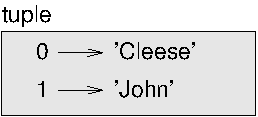
\includegraphics[scale=0.8]{figs/tuple1.pdf}}
\caption{State diagram.}
\label{fig.tuple1}
\end{figure}

But in a larger diagram you might want to leave out the
details.  For example, a diagram of the telephone directory might
appear as in Figure~\ref{fig.dict2}.

但是在一个更大的图中,你可能想省去细节。
例如,电话簿的图可能像图\ref{fig.dict2}一样。

\begin{figure}
\centerline
{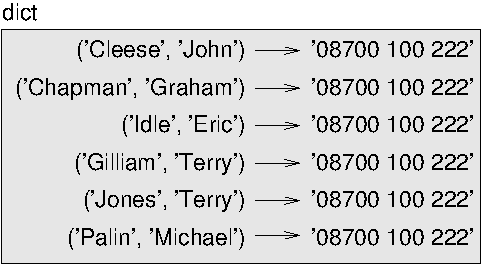
\includegraphics[scale=0.8]{figs/dict2.pdf}}
\caption{State diagram.}
\label{fig.dict2}
\end{figure}

Here the tuples are shown using Python syntax as a graphical
shorthand.

这里,类似速记的方式,使用Python语法显示元组。

The telephone number in the diagram is the complaints line for the
BBC, so please don't call it.

此图中的电话号码是BBC的投诉热线,所以请不要拨打它。



\section{Comparing tuples 元组比较}
\index{comparison!tuple}
\index{tuple!comparison}
\index{sort method}
\index{method!sort}

The relational operators work with tuples and other sequences;
Python starts by comparing the first element from each
sequence.  If they are equal, it goes on to the next elements,
and so on, until it finds elements that differ.  Subsequent
elements are not considered (even if they are really big).

关系运算符可用于元组和其它的序列;Python开始比较每个序列的第一个元素。
如果它们相等,它继续到下一个元素,以此类推,指导发现不同的元素。
后续的元素不被考虑了(即使它们相当的大)。

\begin{verbatim}
>>> (0, 1, 2) < (0, 3, 4)
True
>>> (0, 1, 2000000) < (0, 3, 4)
True
\end{verbatim}
%
The {\tt sort} function works the same way.  It sorts 
primarily by first element, but in the case of a tie, it sorts
by second element, and so on.  

{\tt sort}函数以相同的方式工作。
它主要以第一个元素排序,但是在其相同的情况下,
以第二个元素排序,以此类推。

This feature lends itself to a pattern called {\bf DSU} for 

此特征导致被称作{\bf DSU}的模式,其

\begin{description}

\item[Decorate] a sequence by building a list of tuples
with one or more sort keys preceding the elements from the sequence,

[装饰]一个序列,通过用一个或者更多排序键跟着来自序列的元素来构建一个元组列表,

\item[Sort] the list of tuples, and

[排序]该元组列表,并且

\item[Undecorate] by extracting the sorted elements of the sequence.

[反装饰]通过抽取排好序的序列的元素。

\end{description}

\label{DSU}
\index{DSU pattern}
\index{pattern!DSU}
\index{decorate-sort-undecorate pattern}
\index{pattern!decorate-sort-undecorate}

For example, suppose you have a list of words and you want to
sort them from longest to shortest:

例如,假设你有一个词列表并且你想按照从长到短排序它们:

\begin{verbatim}
def sort_by_length(words):
    t = []
    for word in words:
       t.append((len(word), word))

    t.sort(reverse=True)

    res = []
    for length, word in t:
        res.append(word)
    return res
\end{verbatim}
%
The first loop builds a list of tuples, where each
tuple is a word preceded by its length.

第一个循环构建一个元组列表,其中每个元组是一个单词的长度和该单词。

{\tt sort} compares the first element, length, first, and
only considers the second element to break ties.  The keyword argument
{\tt reverse=True} tells {\tt sort} to go in decreasing order.
\index{keyword argument}
\index{argument!keyword}
\index{traversal}

{\tt sort}首先比较第一个元素,长度,并且只考虑到第二个元素。
实参{\tt reverse=True}告诉{\tt sort}按照降序排序。

The second loop traverses the list of tuples and builds a list of
words in descending order of length.

第二个循环遍历元组列表并且构建一个以长度降序排列的单词列表。

\begin{exercise}

In this example, ties are broken by comparing words, so words
with the same length appear in reverse alphabetical order.  For other
applications you might want to break ties at random.  Modify
this example so that words with the same length appear in
random order.  Hint: see the {\tt random} function in the
{\tt random} module.
Solution: \url{http://thinkpython.com/code/unstable_sort.py}.

\index{random module}
\index{module!random}
\index{random function}
\index{function!random}

\end{exercise}


\section{Sequences of sequences 序列的序列}
\index{sequence}

I have focused on lists of tuples, but almost all of the examples in
this chapter also work with lists of lists, tuples of tuples, and
tuples of lists.  To avoid enumerating the possible combinations, it
is sometimes easier to talk about sequences of sequences.

到现在我一直专注于元组的列表,但是本章中几乎所有的例子也适用于列表的列表,
元组的元组以及列表的元组。为了避免列举所有可能的组合,
讨论序列的序列有时候比较容易。

In many contexts, the different kinds of sequences (strings, lists and
tuples) can be used interchangeably.  So how and why do you choose one
over the others?
\index{string}
\index{list}
\index{tuple}
\index{mutability}
\index{immutability}

在许多情况下,不同类型的序列(字符串、列表和元组)可以被互换使用。
所以如何以及为什么你选择一个而不是其它的呢?

To start with the obvious, strings are more limited than other
sequences because the elements have to be characters.  They are
also immutable.  If you need the ability to change the characters
in a string (as opposed to creating a new string), you might
want to use a list of characters instead.

从明显的开始,字符串比其它的序列更受限,因为元素必须是字符。
它们也是不可变的。如果你需要改变字符串中字符的能力(相对生成一个新的字符串),
你可能想使用字符列表代替。

Lists are more common than tuples, mostly because they are mutable.
But there are a few cases where you might prefer tuples:

列表比元组更一般,主要是因为它们是可变的。
但是也有一些情况你可能更喜欢用元组:

\begin{enumerate}

\item In some contexts, like a {\tt return} statement, it is
syntactically simpler to create a tuple than a list.  In other
contexts, you might prefer a list.

在一些情况下,如{\tt return}语句,生成一个元组比生成一个列表语法更简单。
在其它情况下,你可能倾向于列表。

\item If you want to use a sequence as a dictionary key, you
have to use an immutable type like a tuple or string.

如果你想使用一个序列作为字典的键,那么你必须使用一个类似元组和字符串的不可变类型。

\item If you are passing a sequence as an argument to a function,
using tuples reduces the potential for unexpected behavior
due to aliasing.

如果你正向函数传递一个序列作为实参,那么使用元组以降低由于别名而产生的意外行为的可能性。

\end{enumerate}

Because tuples are immutable, they don't provide methods
like {\tt sort} and {\tt reverse}, which modify existing lists.
But Python provides the built-in functions {\tt sorted}
and {\tt reversed}, which take any sequence as a parameter
and return a new list with the same elements in a different
order.
\index{sorted function}
\index{function!sorted}
\index{reversed function}
\index{function!reversed}

因为元组是不可变的,所以它们不提供类似{\tt sort}和{\tt reverse}的方法,
其改变已有的列表。但是Python提供内建函数{\tt sorted}和{\tt reversed},
其接受任意序列作为形参并返回一个新的相同元素,不同顺序的列表。


\section{Debugging 调试}
\index{debugging}
\index{data structure}
\index{shape error}
\index{error!shape}

Lists, dictionaries and tuples are known generically as {\bf data
  structures}; in this chapter we are starting to see compound data
structures, like lists of tuples, and dictionaries that contain tuples
as keys and lists as values.  Compound data structures are useful, but
they are prone to what I call {\bf shape errors}; that is, errors
caused when a data structure has the wrong type, size or composition.
For example, if you are expecting a list with one integer and I
give you a plain old integer (not in a list), it won't work.
\index{structshape module}
\index{module!structshape}

列表、字典和元组通常被看做{\bf 数据结构(data structures)};
本章中我们正开始看到合成数据结构,如元组的列表,
元组作为键、列表作为值的字典。
合成数据结构很有用,但是它们倾向产生我称作的{\bf 形状错误(shape errors)};
也就是,当一个数据结构有错误的类型、大小或组合时引起的错误。
例如,如果你期望一个具有一个整数的列表并且我给你一个整数(非列表),
它将不会工作。

% TODO: structshape is now part of Swampy

To help debug these kinds of errors, I have written a module
called {\tt structshape} that provides a function, also called
{\tt structshape}, that takes any kind of data structure as
an argument and returns a string that summarizes its shape.
You can download it from \url{http://thinkpython.com/code/structshape.py}

为了帮助调试这些类型的错误,我写了一个被称作{\tt structshape}的模块,
其提供一个函数,也称作{\tt structshape},其接受任意类型的数据结构作为实参
并返回一个字符串,其简要说明它的形状。
你可以从\url{http://thinkpython.com/code/structshape.py}下载它。

Here's the result for a simple list:

这是一个简单列表的结果:

\begin{verbatim}
>>> from structshape import structshape
>>> t = [1,2,3]
>>> print structshape(t)
list of 3 int
\end{verbatim}
%
A fancier program might write ``list of 3 int{\em s},'' but it
was easier not to deal with plurals.  Here's a list of lists:

一个更有想象力的程序可能写出``list of 3 int{\em s}'',
但是不处理复数更简单。这是一个列表的列表:

\begin{verbatim}
>>> t2 = [[1,2], [3,4], [5,6]]
>>> print structshape(t2)
list of 3 list of 2 int
\end{verbatim}
%
If the elements of the list are not the same type,
{\tt structshape} groups them, in order, by type:

如果列表的元素类型不同,{\tt structshape}将它们按顺序按类型分组:

\begin{verbatim}
>>> t3 = [1, 2, 3, 4.0, '5', '6', [7], [8], 9]
>>> print structshape(t3)
list of (3 int, float, 2 str, 2 list of int, int)
\end{verbatim}
%
Here's a list of tuples:

这是一个元组的列表:

\begin{verbatim}
>>> s = 'abc'
>>> lt = zip(t, s)
>>> print structshape(lt)
list of 3 tuple of (int, str)
\end{verbatim}
%
And here's a dictionary with 3 items that map integers to strings.

这是一个具有3个项的字典,其从整数映射到字符串。

\begin{verbatim}
>>> d = dict(lt) 
>>> print structshape(d)
dict of 3 int->str
\end{verbatim}
%
If you are having trouble keeping track of your data structures,
{\tt structshape} can help.

如果你跟踪你的数据结构有困难,{\tt structshape}能帮你。


\section{Glossary 术语表}

\begin{description}

\item[tuple(元组):] An immutable sequence of elements.
\index{tuple}

\item[tuple assignment(元组赋值):] An assignment with a sequence on the
right side and a tuple of variables on the left.  The right
side is evaluated and then its elements are assigned to the
variables on the left.
\index{tuple assignment}
\index{assignment!tuple}

\item[gather(汇集):] The operation of assembling a variable-length
argument tuple.
\index{gather}

\item[scatter(分散):] The operation of treating a sequence as a list of
arguments.
\index{scatter}

\item[DSU:] Abbreviation of ``decorate-sort-undecorate,'' a
pattern that involves building a list of tuples, sorting, and
extracting part of the result.
\index{DSU pattern}

\item[data structure(数据结构):] A collection of related values, often
organized in lists, dictionaries, tuples, etc.
\index{data structure}

\item[shape (of a data structure)(数据结构的形状):] A summary of the type,
size and composition of a data structure.
\index{shape}

\end{description}


\section{Exercises}

\begin{exercise}

Write a function called \verb"most_frequent" that takes a string and
prints the letters in decreasing order of frequency.  Find text
samples from several different languages and see how letter frequency
varies between languages.  Compare your results with the tables at
\url{http://en.wikipedia.org/wiki/Letter_frequencies}.  Solution:
\url{http://thinkpython.com/code/most_frequenct.py}.  \index{letter
  frequency} \index{frequency!letter}

\end{exercise}


\begin{exercise}
\label{anagrams}
\index{anagram set}
\index{set!anagram}

More anagrams!

\begin{enumerate}

\item Write a program
that reads a word list from a file (see Section~\ref{wordlist}) and
prints all the sets of words that are anagrams.

Here is an example of what the output might look like:

\begin{verbatim}
['deltas', 'desalt', 'lasted', 'salted', 'slated', 'staled']
['retainers', 'ternaries']
['generating', 'greatening']
['resmelts', 'smelters', 'termless']
\end{verbatim}
%
Hint: you might want to build a dictionary that maps from a
set of letters to a list of words that can be spelled with those
letters.  The question is, how can you represent the set of
letters in a way that can be used as a key?

\item Modify the previous program so that it prints the largest set
of anagrams first, followed by the second largest set, and so on.
\index{Scrabble}
\index{bingo}

\item In Scrabble a ``bingo'' is when you play all seven tiles in
your rack, along with a letter on the board, to form an eight-letter
word.  What set of 8 letters forms the most possible bingos?
Hint: there are seven.

% (7, ['angriest', 'astringe', 'ganister', 'gantries', 'granites',
% 'ingrates', 'rangiest'])

Solution: \url{http://thinkpython.com/code/anagram_sets.py}.

\end{enumerate}
\end{exercise}

\begin{exercise}
\index{metathesis}

Two words form a ``metathesis pair'' if you can transform one into the
other by swapping two letters; for example, ``converse'' and
``conserve.''  Write a program that finds all of the metathesis pairs
in the dictionary.  Hint: don't test all pairs of words, and don't
test all possible swaps.  Solution: \url{http://thinkpython.com/code/metathesis.py}.
Credit: This exercise is inspired by an example at \url{http://puzzlers.org}.

\end{exercise}



\begin{exercise}
\index{Car Talk}
\index{Puzzler}

Here's another Car Talk Puzzler
(\url{http://www.cartalk.com/content/puzzler/transcripts/200651}):

\begin{quote}
What is the longest English word, that remains a valid English word,
as you remove its letters one at a time?

Now, letters can be removed from either end, or the middle, but you
can't rearrange any of the letters. Every time you drop a letter, you
wind up with another English word. If you do that, you're eventually
going to wind up with one letter and that too is going to be an
English word---one that's found in the dictionary. I want to know
what's the longest word and how many letters does it
have?

I'm going to give you a little modest example: Sprite. Ok? You start
off with sprite, you take a letter off, one from the interior of the
word, take the r away, and we're left with the word spite, then we
take the e off the end, we're left with spit, we take the s off, we're
left with pit, it, and I.
\end{quote}
\index{reducible word}
\index{word, reducible}

Write a program to find all words that can be reduced in this way,
and then find the longest one.

This exercise is a little more challenging than most, so here are
some suggestions:

\begin{enumerate}

\item You might want to write a function that takes a word and
  computes a list of all the words that can be formed by removing one
  letter.  These are the ``children'' of the word.
\index{recursive definition}
\index{definition!recursive}

\item Recursively, a word is reducible if any of its children
are reducible.  As a base case, you can consider the empty
string reducible.

\item The wordlist I provided, {\tt words.txt}, doesn't
contain single letter words.  So you might want to add
``I'', ``a'', and the empty string.

\item To improve the performance of your program, you might want
to memoize the words that are known to be reducible.

\end{enumerate}

Solution: \url{http://thinkpython.com/code/reducible.py}.

\end{exercise}




%\begin{exercise}
%\url{http://en.wikipedia.org/wiki/Word_Ladder}
%\end{exercise}




\chapter{Case study: data structure selection 案例学习:数据结构选择}

\section{Word frequency analysis 词频分析}
\label{analysis}

As usual, you should at least attempt the following exercises
before you read my solutions.

和往常一样,在你阅读我的答案之前,你至少应该尝试解决一下下面的习题。

\begin{exercise}

Write a program that reads a file, breaks each line into
words, strips whitespace and punctuation from the words, and
converts them to lowercase.
\index{string module}
\index{module!string}

写一个程序,读取一个文件,每一行是一个单词,
删掉单词中的空格和标点,并且将它们转化为小写字母。

Hint: The {\tt string} module provides strings named {\tt whitespace},
which contains space, tab, newline, etc., and {\tt
  punctuation} which contains the punctuation characters.  Let's see
if we can make Python swear:

提示:{\tt string}模块提供了名为{\tt whitespace}的字符串,
其包括空格、制表符、新行等等,以及{\tt punctuation},
其包括标点字符。让我们看一下是否我们能让Python说脏话:

\begin{verbatim}
>>> import string
>>> print string.punctuation
!"#$%&'()*+,-./:;<=>?@[\]^_`{|}~
\end{verbatim}
%
Also, you might consider using the string methods {\tt strip},
{\tt replace} and {\tt translate}.
\index{strip method}
\index{method!strip}
\index{replace method}
\index{method!replace}
\index{translate method}
\index{method!translate}

同时,你可能需要考虑使用字符串方法{\tt strip}、{\tt replace}和{\tt translate}。

\end{exercise}


\begin{exercise}
\index{Project Gutenberg 古腾堡项目}

Go to Project Gutenberg (\url{gutenberg.org}) and download 
your favorite out-of-copyright book in plain text format.
\index{plain text}
\index{text!plain}

前往古腾堡项目(\url{gutenberg.org})以纯文本格式下载你喜欢的版权已过期的图书。

Modify your program from the previous exercise to read the book
you downloaded, skip over the header information at the beginning
of the file, and process the rest of the words as before.

修改你前面习题的程序来读取你下载的书,
跳过文件开始的头部信息,并如前面一样处理其余的单词。

Then modify the program to count the total number of words in
the book, and the number of times each word is used.
\index{word frequency}
\index{frequency!word}

然后修改程序来计算书中单词的总数,
以及每个单词被使用的次数。

Print the number of different words used in the book.  Compare
different books by different authors, written in different eras.
Which author uses the most extensive vocabulary?

打印该书使用的不同单词的数目。
比较不同年代,不同作者写的不同的书。
哪个作者使用的词汇最大?

\end{exercise}


\begin{exercise}

Modify the program from the previous exercise to print the
20 most frequently-used words in the book.

修改前面习题的程序来打印该书中最常使用的20个单词。

\end{exercise}


\begin{exercise}

Modify the previous program to read a word list (see
Section~\ref{wordlist}) and then print all the words in the book that
are not in the word list.  How many of them are typos?  How many of
them are common words that {\em should} be in the word list, and how
many of them are really obscure?

修改前面的程序来读取一个词表(见\ref{wordlist}节),
然后打印书中所有没有出现在该词表中的单词。
它们中有多少是拼写错误的?
有多少是词表中应该包括的常用词?
有多少是生僻词?

\end{exercise}


\section{Random numbers 随机数}
\index{random number}
\index{number, random}
\index{deterministic}
\index{pseudorandom}

Given the same inputs, most computer programs generate the same
outputs every time, so they are said to be {\bf deterministic}.
Determinism is usually a good thing, since we expect the same
calculation to yield the same result.  For some applications, though,
we want the computer to be unpredictable.  Games are an obvious
example, but there are more.

给定相同的输入,大多数计算机程序每次生成相同的输出,
所以它们被称作{\bf 确定性的(deterministic)}。
确定性通常是个好东西,因为我们期望相同的计算产生相同的结果。
然而,对于有些应用,我们期望计算机不可预知。
有戏是一个明显的例子,但是有更多的例子。

Making a program truly nondeterministic turns out to be not so easy,
but there are ways to make it at least seem nondeterministic.  One of
them is to use algorithms that generate {\bf pseudorandom} numbers.
Pseudorandom numbers are not truly random because they are generated
by a deterministic computation, but just by looking at the numbers it
is all but impossible to distinguish them from random.
\index{random module}
\index{module!random}

让一个程序真的非确定性并不容易,但是有办法使它看起来是非确定的。
其中之一是使用生成{\bf 伪随机(pseudorandom)}数算法。
伪随机数不是真正的随机,因为它们由一个确定性的计算生成,
但是仅看其生成的数字,不可能将它们和随机生成的相区分开。

The {\tt random} module provides functions that generate
pseudorandom numbers (which I will simply call ``random'' from
here on).
\index{random function}
\index{function!random}

{\tt random}模块提供生成伪随机数的函数(从此之后,我将简单的称其为``随机'')。

The function {\tt random} returns a random float
between 0.0 and 1.0 (including 0.0 but not 1.0).  Each time you
call {\tt random}, you get the next number in a long series.  To see a
sample, run this loop:

函数{\tt random}返回一个0.0到1.0之间的随机浮点数(包括0.0,但是不包括1.0)。
每次你调用{\tt random},你获得一个长序列中的下一个树。
为了看一个例子,运行此循环:

\begin{verbatim}
import random

for i in range(10):
    x = random.random()
    print x
\end{verbatim}
%
The function {\tt randint} takes parameters {\tt low} and
{\tt high} and returns an integer between {\tt low} and
{\tt high} (including both).
\index{randint function}
\index{function!randint}

函数{\tt randint}接受参数{\tt low}和{\tt high},
并返回一个{\tt low}和{\tt high}之间的整数(两个都包括)。

\begin{verbatim}
>>> random.randint(5, 10)
5
>>> random.randint(5, 10)
9
\end{verbatim}
%
To choose an element from a sequence at random, you can use
{\tt choice}:
\index{choice function}
\index{function!choice}

为了从一个序列中随机的选择一个元素,你可以使用{\tt choice}:

\begin{verbatim}
>>> t = [1, 2, 3]
>>> random.choice(t)
2
>>> random.choice(t)
3
\end{verbatim}
%
The {\tt random} module also provides functions to generate
random values from continuous distributions including
Gaussian, exponential, gamma, and a few more.


{\tt random}模块也提供从包括高斯、指数、伽马以及更多连续分布中生成随机值的函数。

\begin{exercise}
\index{histogram!random choice}

Write a function named \verb"choose_from_hist" that takes
a histogram as defined in Section~\ref{histogram} and returns a 
random value from the histogram, chosen with probability
in proportion to frequency.  For example, for this histogram:

写一个名为\verb"choose_from_hist"的函数,
其接受一个如\ref{histogram}节定义的直方图,
并从该直方图中返回一个随机值,其选择概率和频率成正比。
例如,对于此直方图:

\begin{verbatim}
>>> t = ['a', 'a', 'b']
>>> hist = histogram(t)
>>> print hist
{'a': 2, 'b': 1}
\end{verbatim}
%
your function should return {\tt 'a'} with probability $2/3$ and {\tt 'b'}
with probability $1/3$.

你的函数应该返回{\tt 'a'}和概率$2/3$以及{\tt 'b'}和概率$1/3$。

\end{exercise}


\section{Word histogram 单词直方图}

You should attempt the previous exercises before you go on.
You can download my solution from
 \url{http://thinkpython.com/code/analyze_book.py}.  You will
also need \url{http://thinkpython.com/code/emma.txt}.

在你继续之前,你应该尝试前面的习题。
你可以从\url{http://thinkpython.com/code/analyze_book.py}下载我的答案。
你也需要\url{http://thinkpython.com/code/emma.txt}。

Here is a program that reads a file and builds a histogram of the
words in the file:
\index{histogram!word frequencies}

这是一个读取一个文件并建立文件中单词直方图的程序。

\begin{verbatim}
import string

def process_file(filename):
    hist = dict()
    fp = open(filename)
    for line in fp:
        process_line(line, hist)
    return hist

def process_line(line, hist):
    line = line.replace('-', ' ')
    
    for word in line.split():
        word = word.strip(string.punctuation + string.whitespace)
        word = word.lower()

        hist[word] = hist.get(word, 0) + 1

hist = process_file('emma.txt')
\end{verbatim}
%
This program reads {\tt emma.txt}, which contains the text of {\em
  Emma} by Jane Austen.
\index{Austin, Jane}

改程序读取{\tt emma.txt},其包括Jane Austen写的{\em Emma}的文本。

\verb"process_file" loops through the lines of the file,
passing them one at a time to \verb"process_line".  The histogram
{\tt hist} is being used as an accumulator.
\index{accumulator!histogram}
\index{traversal}

\verb"process_file"循环读取每行文件,每次把它们传递给\verb"process_line"。
直方图{\tt hist}被用作一个累加器。

\verb"process_line" uses the string method {\tt replace} to replace
hyphens with spaces before using {\tt split} to break the line into a
list of strings.  It traverses the list of words and uses {\tt strip}
and {\tt lower} to remove punctuation and convert to lower case.  (It
is a shorthand to say that strings are ``converted;'' remember that
string are immutable, so methods like {\tt strip} and {\tt lower}
return new strings.)

在使用{\tt split}将一行文件分成一个字符串列表之前,
\verb"process_line"使用字符串{\tt replace}方法来用空格替换连字符。
它遍历单词的列表,并使用{\tt strip}和{\tt lower}来删除标点以及转化为小写。
(简称字符串被``转化'';记住字符串是不可变的,
所以类似{\tt strip}和{\tt lower}的方法返回新的字符串。)

Finally, \verb"process_line" updates the histogram by creating a new
item or incrementing an existing one.
\index{update!histogram}

最后,\verb"process_line"通过生成一个新的项或者递增一个已有的项来更新直方图。

To count the total number of words in the file, we can add up
the frequencies in the histogram:

为了计算文件中单词的总数,我们可以累加直方图中的频率:

\begin{verbatim}
def total_words(hist):
    return sum(hist.values())
\end{verbatim}
%
The number of different words is just the number of items in
the dictionary:

不同单词的数量恰好是词典中项的数目:

\begin{verbatim}
def different_words(hist):
    return len(hist)
\end{verbatim}
%
Here is some code to print the results:

这是打印结果的代码:

\begin{verbatim}
print 'Total number of words:', total_words(hist)
print 'Number of different words:', different_words(hist)
\end{verbatim}
%
And the results:

结果是:

\begin{verbatim}
Total number of words: 161080
Number of different words: 7214
\end{verbatim}
%

\section{Most common words 最常用单词}
\index{DSU pattern}
\index{pattern!DSU}

To find the most common words, we can apply the DSU pattern;
\verb"most_common" takes a histogram and returns a list of
word-frequency tuples, sorted in reverse order by frequency:

为了找到最常用的单词,我们可以应用DSU模式;
\verb"most_common"接受一个直方图并且返回一个
以频率倒序排列的单词-频率元组列表:

\begin{verbatim}
def most_common(hist):
    t = []
    for key, value in hist.items():
        t.append((value, key))

    t.sort(reverse=True)
    return t
\end{verbatim}
%
Here is a loop that prints the ten most common words:

这是一个打印10个最常用单词的循环:

\begin{verbatim}
t = most_common(hist)
print 'The most common words are:'
for freq, word in t[0:10]:
    print word, '\t', freq
\end{verbatim}
%
And here are the results from {\em Emma}:

这是来自{\em Emma}的结果:

\begin{verbatim}
The most common words are:
to 	5242
the 	5205
and 	4897
of 	4295
i 	3191
a 	3130
it 	2529
her 	2483
was 	2400
she 	2364
\end{verbatim}
%

\section{Optional parameters 可选形参}
\index{optional parameter}
\index{parameter!optional}

We have seen built-in functions and methods that take a variable
number of arguments.  It is possible to write user-defined functions
with optional arguments, too.  For example, here is a function that
prints the most common words in a histogram

我们已经见过接受可变数目实参的函数和方法了。
写出具有可选实参的用户自定义函数也是有可能的。
例如,这是一个打印直方图中最常见单词的函数。

\begin{verbatim}
def print_most_common(hist, num=10):
    t = most_common(hist)
    print 'The most common words are:'
    for freq, word in t[:num]:
        print word, '\t', freq
\end{verbatim}

The first parameter is required; the second is optional.
The {\bf default value} of {\tt num} is 10.
\index{default value}
\index{value!default}

第一个形参是必须的;第二个是可选的。
{\tt num}的{\bf 默认值(default value)}是10.

If you only provide one argument:

\begin{verbatim}
print_most_common(hist)
\end{verbatim}

{\tt num} gets the default value.  If you provide two arguments:

{\tt num}获得默认值。如果你提供两个实参:

\begin{verbatim}
print_most_common(hist, 20)
\end{verbatim}

{\tt num} gets the value of the argument instead.  In other
words, the optional argument {\bf overrides} the default value.
\index{override}

{\tt num}获得实参的值。换句话说,可选实参{\bf 覆盖(overrides)}了默认值。

If a function has both required and optional parameters, all
the required parameters have to come first, followed by the
optional ones.

如果一个函数必选和可选两类形参,则所有的必选形参必须首先出现,
后面跟着可选的。

\section{Dictionary subtraction 字典差集}
\index{dictionary!subtraction}
\index{subtraction!dictionary}

Finding the words from the book that are not in the word list
from {\tt words.txt} is a problem you might recognize as set
subtraction; that is, we want to find all the words from one
set (the words in the book) that are not in another set (the
words in the list).

从书中找到所有没出现在词表{\tt words.txt}中的单词是一个差集问题。
也就是,我们想从一个集合中(书中的单词)找到所有没出现在另一个集合中
(列表中的单词)的单词。

{\tt subtract} takes dictionaries {\tt d1} and {\tt d2} and returns a
new dictionary that contains all the keys from {\tt d1} that are not
in {\tt d2}.  Since we don't really care about the values, we
set them all to None.

{\tt subtract}接受词典{\tt d1}和{\tt d2},并返回一个新的词典,
其包括{\tt d1}中的所有没出现在{\tt d2}中的键。
既然我们并不真正关心值,我们将它们都设为None。

\begin{verbatim}
def subtract(d1, d2):
    res = dict()
    for key in d1:
        if key not in d2:
            res[key] = None
    return res
\end{verbatim}
%
To find the words in the book that are not in {\tt words.txt},
we can use \verb"process_file" to build a histogram for
{\tt words.txt}, and then subtract:

为了找到书中的没有出现在{\tt words.txt}中的单词,
我们可以使用\verb"process_file"来为{\tt words.txt}构建一个直方图,
然后subtract:

\begin{verbatim}
words = process_file('words.txt')
diff = subtract(hist, words)

print "The words in the book that aren't in the word list are:"
for word in diff.keys():
    print word,
\end{verbatim}
%
Here are some of the results from {\em Emma}:

这是来自{\em Emma}的一些结果:

\begin{verbatim}
The words in the book that aren't in the word list are:
 rencontre jane's blanche woodhouses disingenuousness 
friend's venice apartment ...
\end{verbatim}
%
Some of these words are names and possessives.  Others, like
``rencontre,'' are no longer in common use.  But a few are common
words that should really be in the list!

这些单词一些是名字和所有歌。另外的,如``rencontre''不是常用单词。
但是有一些确实是真的应该包括在列表中的常用单词。

\begin{exercise}
\index{set}
\index{type!set}

Python provides a data structure called {\tt set} that provides many
common set operations.  Read the documentation at
\url{http://docs.python.org/lib/types-set.html} and write a program
that uses set subtraction to find words in the book that are not in
the word list.  Solution: \url{http://thinkpython.com/code/analyze_book2.py}.

\end{exercise}


\section{Random words 随机单词}
\label{randomwords}
\index{histogram!random choice}

To choose a random word from the histogram, the simplest algorithm
is to build a list with multiple copies of each word, according
to the observed frequency, and then choose from the list:

为了从直方图中随机选择一个单词,最简单的算法是创建一个列表,
其中根据其出现的频率,每个单词都有多个拷贝,
然后从该列表中选择:

\begin{verbatim}
def random_word(h):
    t = []
    for word, freq in h.items():
        t.extend([word] * freq)

    return random.choice(t)
\end{verbatim}
%
The expression {\tt [word] * freq} creates a list with {\tt freq}
copies of the string {\tt word}.  The {\tt extend}
method is similar to {\tt append} except that the argument is
a sequence.

表达式{\tt [word] * freq}生成一个具有{\tt freq}个字符串{\tt word}拷贝的列表。
{\tt extend}方法和{\tt append}类似,除了其实参为一个序列外。

\begin{exercise}
\label{randhist}
\index{algorithm}

This algorithm works, but it is not very efficient; each time you
choose a random word, it rebuilds the list, which is as big as
the original book.  An obvious improvement is to build the list
once and then make multiple selections, but the list is still big.

该算法好使,但是不是很有效;每次你选择一个随机单词,
它都重建列表,其和原来的书一样大。
一个明显的改进是创建列表一次,然后进行多次选择,
但是该列表仍然很大。

An alternative is:

一个替代是:

\begin{enumerate}

\item Use {\tt keys} to get a list of the words in the book.

使用{\tt keys}来获得该书中单词的列表。

\item Build a list that contains the cumulative sum of the word
  frequencies (see Exercise~\ref{cumulative}).  The last item
  in this list is the total number of words in the book, $n$.
  
创建一个包含单词频率累积和的列表(见习题\ref{cumulative})。
此列表的最后一项是书中单词的数目$n$。
  
\item Choose a random number from 1 to $n$.  Use a bisection search
  (See Exercise~\ref{bisection}) to find the index where the random
  number would be inserted in the cumulative sum.
  
选择一个从1到$n$的随机数。使用二分搜索(见习题\ref{bisection})
找到该随机数应该被在累积和中插入的索引。

\item Use the index to find the corresponding word in the word list.

使用该索引从单词列表中找到相应的单词。

\end{enumerate}

Write a program that uses this algorithm to choose a random
word from the book.  Solution: \url{http://thinkpython.com/code/analyze_book3.py}.

写一个使用该算法从书中选择一个随机单词的程序。
答案:\url{http://thinkpython.com/code/analyze_book3.py}。

\end{exercise}



\section{Markov analysis 马尔科夫分析}
\label{markov}
\index{Markov analysis}

If you choose words from the book at random, you can get a
sense of the vocabulary, you probably won't get a sentence:

如果你从书中随机选择单词,那么你会感受到词表的概念,
你可能不会获得一个句子:

\begin{verbatim}
this the small regard harriet which knightley's it most things
\end{verbatim}
%
A series of random words seldom makes sense because there
is no relationship between successive words.  For example, in
a real sentence you would expect an article like ``the'' to
be followed by an adjective or a noun, and probably not a verb
or adverb.

一系列随机单词没有意义,因为相邻的单词没有关系。
例如,在一个真实的句子中,你可能期望``the''后面跟着一个形容词或者名称,
不可能是一个动词或者副词。

One way to measure these kinds of relationships is Markov
analysis, which
characterizes, for a given sequence of words, the probability of the
word that comes next.  For example, the song {\em Eric, the Half a
  Bee} begins:
  
一种衡量这种关系的方法是马尔科夫分析,对于一个给定的单词序列,
其描述了接下来的单词的概率。
例如,歌曲{\em Eric, the Half a Bee}开始是:

\begin{quote}
Half a bee, philosophically, \\
Must, ipso facto, half not be. \\
But half the bee has got to be \\
Vis a vis, its entity. D'you see? \\
\\
But can a bee be said to be \\
Or not to be an entire bee \\
When half the bee is not a bee \\
Due to some ancient injury? \\
\end{quote}
%
In this text,
the phrase ``half the'' is always followed by the word ``bee,''
but the phrase ``the bee'' might be followed by either
``has'' or ``is''.
\index{prefix}
\index{suffix}
\index{mapping}

在此文本中,短语``half the''后面总是跟着单词``bee'',
但是短语``the bee''则可能跟着``has''或者``is''。

The result of Markov analysis is a mapping from each prefix
(like ``half the'' and ``the bee'') to all possible suffixes
(like ``has'' and ``is'').
\index{random text}
\index{text!random}

马尔科夫分析的结果是从每个前缀(如``half the''和``the bee'')
映射到所有可能的后缀(如``has''和``is'')。

Given this mapping, you can generate a random text by
starting with any prefix and choosing at random from the
possible suffixes.  Next, you can combine the end of the
prefix and the new suffix to form the next prefix, and repeat.

给定此映射,你可以以任意前缀开始并从可能的后缀中随机选择一个来生成一个随机文本。
接下来,你可以组合前缀的结尾和新的后缀形参下一个前缀,并重复下去。

For example, if you start with the prefix ``Half a,'' then the
next word has to be ``bee,'' because the prefix only appears
once in the text.  The next prefix is ``a bee,'' so the
next suffix might be ``philosophically,'' ``be'' or ``due.''

例如,如果你以前缀``Half a''开始,然后下一个但是必须是``bee'',
因为此前缀在文本中仅出现一次。下一个前缀是``a bee'',
所以下一个后缀可能是``philosophically'',``be''或``due''。

In this example the length of the prefix is always two, but
you can do Markov analysis with any prefix length.  The length
of the prefix is called the ``order'' of the analysis.

此例中,前缀的长度总是2,但是你可以以任意前缀长度进行马尔科夫分析。
前缀的长度被称作此分析的``阶''。

\begin{exercise}

Markov analysis:

马尔科夫分析:

\begin{enumerate}

\item Write a program to read a text from a file and perform Markov
analysis.  The result should be a dictionary that maps from
prefixes to a collection of possible suffixes.  The collection
might be a list, tuple, or dictionary; it is up to you to make
an appropriate choice.  You can test your program with prefix
length two, but you should write the program in a way that makes
it easy to try other lengths.

写一个程序,从一个文件中读取文本并执行马尔科夫分析。
结果应该是一个字典,其从前缀映射到一个可能的后缀集合。
此集合可以是一个列表、元组或字典;一切取决于你以做出合适的选择。
你可以用长度为2的前缀进行测试,但是你应该让此程序很容易的支持其它长度。

\item Add a function to the previous program to generate random text
based on the Markov analysis.  Here is an example from {\em Emma}
with prefix length 2:

在前面的程序中加一个函数,基于马尔科夫分析生成随机文本。
这是来自{\em Emma}的前缀为2的一个例子:

\begin{quote}
He was very clever, be it sweetness or be angry, ashamed or only
amused, at such a stroke. She had never thought of Hannah till you
were never meant for me?" "I cannot make speeches, Emma:" he soon cut
it all himself.
\end{quote}

For this example, I left the punctuation attached to the words.
The result is almost syntactically correct, but not quite.
Semantically, it almost makes sense, but not quite.

对于这个例子,我保留了附在词后面的标点符号。
结果几乎是语法正确的,但不完全。
语义上讲,它几乎有意义,但也不完全。

What happens if you increase the prefix length?  Does the random
text make more sense?
\index{mash-up}

如果你增加前缀的长度,会发生什么?
随机文本更有意义是么?

\item Once your program is working, you might want to try a mash-up:
if you analyze text from two or more books, the random
text you generate will blend the vocabulary and phrases from
the sources in interesting ways.

一旦你的程序工作,你可能想尝试一下混搭:
如果你来自两本或更多书的文本,
你生成的随机文本将以有趣的方式混合来自不同源的词表和短语。

\end{enumerate}

Credit: This case study is based on an example from Kernighan and
Pike, {\em The Practice of Programming}, Addison-Wesley, 1999.

声明:此案例学习基于来自Kernighan and Pike, {\em The Practice of Programming}, Addison-Wesley, 1999.
的一个示例。

\end{exercise}

You should attempt this exercise before you go on; then you can
download my solution from \url{http://thinkpython.com/code/markov.py}.  You
will also need \url{http://thinkpython.com/code/emma.txt}.

在你继续之前,你应该尝试此习题;
你可以从\url{http://thinkpython.com/code/markov.py}下载我的答案。
你也需要\url{http://thinkpython.com/code/emma.txt}。

\section{Data structures 数据结构}
\index{data structure}

Using Markov analysis to generate random text is fun, but there is
also a point to this exercise: data structure selection.  In your
solution to the previous exercises, you had to choose:

使用马尔科夫分析生成随机文本很有趣,
但是对此习题还有一点需要注意:数据结构选择。
在你的解决方案中,你不得不选择:

\begin{itemize}

\item How to represent the prefixes.

如何表示前缀。

\item How to represent the collection of possible suffixes.

如何表示可能后缀的集合。

\item How to represent the mapping from each prefix to
the collection of possible suffixes.

如何表示从前缀到可能后缀集合的映射。

\end{itemize}

Ok, the last one is the easy; the only mapping type we have
seen is a dictionary, so it is the natural choice.

好的,最后一个很简单;我们曾见过的唯一的映射是字典,
所以它是很自然的选择。

For the prefixes, the most obvious options are string,
list of strings, or tuple of strings.  For the suffixes,
one option is a list; another is a histogram (dictionary).
\index{implementation}

对于前缀,最明显的选项是字符串、字符串列表或者字符串元组。
对于后缀,一个选择是列表;另一个是直方图(字典)。

How should you choose?  The first step is to think about
the operations you will need to implement for each data structure.
For the prefixes, we need to be able to remove words from
the beginning and add to the end.  For example, if the current
prefix is ``Half a,'' and the next word is ``bee,'' you need
to be able to form the next prefix, ``a bee.''
\index{tuple!as key in dictionary}

你如何选择呢?
第一步是考虑对每个数据结构你需要实现的操作。
对于前缀,我们需要能从从开始删除单词并在最后加入单词。
例如,如果当前的前缀是``Half a'',下一个词是``bee'',
你需要能构成下一个前缀``a bee''。

Your first choice might be a list, since it is easy to add
and remove elements, but we also need to be able to use the
prefixes as keys in a dictionary, so that rules out lists.
With tuples, you can't append or remove, but you can use
the addition operator to form a new tuple:

你的第一个选择可能是列表,因为它能很容易的增加和删除元素,
但是我们也需要让前缀作为字典的键,因此淘汰了列表。
使用元组,你不能追加或删除,
但是你能使用额外的运算符来形成一个新的元组:

\begin{verbatim}
def shift(prefix, word):
    return prefix[1:] + (word,)
\end{verbatim}
%
{\tt shift} takes a tuple of words, {\tt prefix}, and a string, 
{\tt word}, and forms a new tuple that has all the words
in {\tt prefix} except the first, and {\tt word} added to
the end.

{\tt shift}接受一个单词元组{\tt prefix}和一个字符串{\tt word},
并形成一个新的元组,其具有{\tt prefix}中除第一个单词外的全部单词,
然后在结尾增加{\tt word}。

For the collection of suffixes, the operations we need to
perform include adding a new suffix (or increasing the frequency
of an existing one), and choosing a random suffix.

对于后缀的集合,我们需要执行的运算包括增加一个新的后缀
(或者增加一个已有后缀的频度),并选择一个随机后缀。

Adding a new suffix is equally easy for the list implementation
or the histogram.  Choosing a random element from a list
is easy; choosing from a histogram is harder to do
efficiently (see Exercise~\ref{randhist}).

对于列表或者直方图,增加一个新的后缀一样容易。
从列表中选择一个随机元素很容易;
从一个直方图中有效的选择有一些难(见习题\ref{randhist})。

So far we have been talking mostly about ease of implementation,
but there are other factors to consider in choosing data structures.
One is run time.  Sometimes there is a theoretical reason to expect
one data structure to be faster than other; for example, I mentioned
that the {\tt in} operator is faster for dictionaries than for lists,
at least when the number of elements is large.

目前为止,我们主要讨论实现的难易,
但是选择数据结构还有其它的因素。一个是运行时间。
有时,一个数据结构比另一个快有理论原因;
例如,我提到过{\tt in}运算符对于字典比对列表要快,
至少当元素的数目很大的时候。

But often you don't know ahead of time which implementation will
be faster.  One option is to implement both of them and see which
is better.  This approach is called {\bf benchmarking}.  A practical
alternative is to choose the data structure that is
easiest to implement, and then see if it is fast enough for the
intended application.  If so, there is no need to go on.  If not,
there are tools, like the {\tt profile} module, that can identify
the places in a program that take the most time.
\index{benchmarking}
\index{profile module}
\index{module!profile}

但是通常你事先不知道哪个实现更快。
一个选择是两个都实现,然后再看哪个更快。
此方法被称作{\bf 基准测试(benchmarking)}。
一个实用的选择是选择最容易实现的数据结构,
然后看它对于拟定的应用是否足够快。
如果是的话,就不需要继续了。
如果不是,有一些工具,如{\tt profile}模块,
其能识别一个程序中哪处最耗时。

The other factor to consider is storage space.  For example, using a
histogram for the collection of suffixes might take less space because
you only have to store each word once, no matter how many times it
appears in the text.  In some cases, saving space can also make your
program run faster, and in the extreme, your program might not run at
all if you run out of memory.  But for many applications, space is a
secondary consideration after run time.

另外考虑的因素是存储空间。例如,对后缀集合使用直方图可能用更少的空间,
因为无论一个单词在文本中出现多少次,你只需要存储它一次。
在一些情况下,节省空间也能让你的程序更快,极端情况下,
如果内存溢出,你的程序可能根本不能运行。
但是对于许多应用,空间是运行时间之后的第二位考虑。

One final thought: in this discussion, I have implied that
we should use one data structure for both analysis and generation.  But
since these are separate phases, it would also be possible to use one
structure for analysis and then convert to another structure for
generation.  This would be a net win if the time saved during
generation exceeded the time spent in conversion.

最后一个思考:在此讨论中,我暗示对于分析和生成,
我们应该使用一种数据结构。但是既然这些事分离的步骤,
对于分析使用一种数据结构,然后对生成转到另一种结构也是可能的。
如果生成节省的时间超过了转化花费的时间,这将是一个极大的优势。

\section{Debugging 调试}
\index{debugging}

When you are debugging a program, and especially if you are
working on a hard bug, there are four things to try:

当你正在调试一个程序的时候,特别是如果你正在调试一个很难的错误,
有四件事需要试一下:

\begin{description}

\item[reading:] Examine your code, read it back to yourself, and
check that it says what you meant to say.

读:检查你的代码,你自己回头读它,并且检查它说的是否是你想说的。

\item[running:] Experiment by making changes and running different
versions.  Often if you display the right thing at the right place
in the program, the problem becomes obvious, but sometimes you have to
spend some time to build scaffolding.

运行:通过修改和运行不同的版本来实验。
通常,如果在程序中,你在正确的地方显示正确的东西,
问题变得很明显,但是有时你不得不花些时间创建脚手架。

\item[ruminating:] Take some time to think!  What kind of error
is it: syntax, runtime, semantic?  What information can you get from
the error messages, or from the output of the program?  What kind of
error could cause the problem you're seeing?  What did you change
last, before the problem appeared?

沉思:花些时间思考!错误的类型是什么:语法、运行时、语义?
你从错误信息或者程序的输出中能获得什么信息?
什么类型的错误能引起你看到的问题?
问题出现前,你最后的修改是什么?

\item[retreating:] At some point, the best thing to do is back
off, undoing recent changes, until you get back to a program that
works and that you understand.  Then you can start rebuilding.

回退:在某种情况下,最好的事情是回退,撤销最近的修改,
直到你回到一个能工作并且你能理解的程序。
然后你可以开始重建。

\end{description}

Beginning programmers sometimes get stuck on one of these activities
and forget the others.  Each activity comes with its own failure
mode.
\index{typographical error}

初级程序员有时陷入这些活动之一,并且忘记了其它的。
每个活动伴随着它自己的故障模式。

For example, reading your code might help if the problem is a
typographical error, but not if the problem is a conceptual
misunderstanding.  If you don't understand what your program does, you
can read it 100 times and never see the error, because the error is in
your head.
\index{experimental debugging}

例如,如果程序是一个拍板错误,读代码可能有帮助,
但是如果问题是概念理解错误,则未必是这样。
如果你不理解你的程序做什么,
你可能读你的程序100遍,并从不会发现错误,
因为错误在你的头脑中。

Running experiments can help, especially if you run small, simple
tests.  But if you run experiments without thinking or reading your
code, you might fall into a pattern I call ``random walk programming,''
which is the process of making random changes until the program
does the right thing.  Needless to say, random walk programming
can take a long time.
\index{random walk programming}
\index{development plan!random walk programming}

运行实验可能会有帮助,特别是如果你运行小的、简单的测试。
但是,如果你不思考或者阅读你的代码而运行实验,
你可能陷入一种被我称作``随机游走编程''的模式中,
这是一个随机修改的过程,直到程序做了正确的事儿。
不用说,随机游走编程会花费很长的时间。

You have to take time to think.  Debugging is like an
experimental science.  You should have at least one hypothesis about
what the problem is.  If there are two or more possibilities, try to
think of a test that would eliminate one of them.

你必须花时间思考。调试类似实验科学。
你应该至少有一个关于问题是什么的假设。
如果有两个或者更多的可能,试着考虑一个能消除其中一个的测试。

Taking a break helps with the thinking.  So does talking.
If you explain the problem to someone else (or even yourself), you
will sometimes find the answer before you finish asking the question.

休息一下有助于帮助思考。讨论也是。
如果你向他人(或者即使你自己)解释问题,
有时你将在说完问题之前找到答案。

But even the best debugging techniques will fail if there are too many
errors, or if the code you are trying to fix is too big and
complicated.  Sometimes the best option is to retreat, simplifying the
program until you get to something that works and that you
understand.

但是,如果有太多的错误或则你正试图修复的代码太大、太复杂,
即使最好的调试技术也会失败。
有时,最好的选择是回退,简化程序,直到你获得一个好使的并且能理解的程序。

Beginning programmers are often reluctant to retreat because
they can't stand to delete a line of code (even if it's wrong).
If it makes you feel better, copy your program into another file
before you start stripping it down.  Then you can paste the pieces
back in a little bit at a time.

初级程序员经常不愿意回退,因为他们不愿意删除一行代码(即使它是错误的)。
如果这让你感觉好些,在你开始删除之前,将你的代码拷贝到另一个文件中。
然后你能一次性把它们粘贴回来。

Finding a hard bug requires reading, running, ruminating, and
sometimes retreating.  If you get stuck on one of these activities,
try the others.

找到一个很难的错误需要阅读、运行、沉思、和时而的回退。
如果你陷入其中的一个活动中,试一下其它的。

\section{Glossary 术语表}

\begin{description}

\item[deterministic(确定性的):] Pertaining to a program that does the same
thing each time it runs, given the same inputs.
\index{deterministic}

\item[pseudorandom(伪随机):] Pertaining to a sequence of numbers that appear
to be random, but are generated by a deterministic program.
\index{pseudorandom}

\item[default value(默认值):] The value given to an optional parameter if no
argument is provided.
\index{default value}

\item[override(覆盖):] To replace a default value with an argument.
\index{override}

\item[benchmarking(基准测试):] The process of choosing between data structures
by implementing alternatives and testing them on a sample of the
possible inputs.  
\index{benchmarking}

\end{description}


\section{Exercises}

\begin{exercise}
\index{word frequency}
\index{frequency!word}
\index{Zipf's law}

The ``rank'' of a word is its position in a list of words
sorted by frequency: the most common word has rank 1, the
second most common has rank 2, etc.

Zipf's law describes a relationship between the ranks and frequencies
of words in natural languages
(\url{http://en.wikipedia.org/wiki/Zipf's_law}).  Specifically, it
predicts that the frequency, $f$, of the word with rank $r$ is:

\[ f = c r^{-s} \]
%
where $s$ and $c$ are parameters that depend on the language and the
text.  If you take the logarithm of both sides of this equation, you
get:
\index{logarithm}

\[ \log f = \log c - s \log r \]
%
So if you plot log $f$ versus log $r$, you should get
a straight line with slope $-s$ and intercept log $c$.

Write a program that reads a text from a file, counts
word frequencies, and prints one line
for each word, in descending order of frequency, with
log $f$ and log $r$.  Use the graphing program of your
choice to plot the results and check whether they form
a straight line.  Can you estimate the value of $s$?

Solution: \url{http://thinkpython.com/code/zipf.py}.  To make the plots, you
might have to install matplotlib (see
\url{http://matplotlib.sourceforge.net/}).
\index{Matplotlib}

\end{exercise}


\chapter{Files 文件}


\section{Persistence 持久化}
\index{file}
\index{type!file}
\index{persistence}

Most of the programs we have seen so far are transient in the
sense that they run for a short time and produce some output,
but when they end, their data disappears.  If you run the program
again, it starts with a clean slate.

目前我们见到的大部分程序都是瞬态的,它们运行一小段时间便输出一些结果。
然而当程序运行结束后,它们的数据就会消失。
如果你重新运行这个程序,它们又会从零开始。

Other programs are {\bf persistent}: they run for a long time
(or all the time); they keep at least some of their data
in permanent storage (a hard drive, for example); and
if they shut down and restart, they pick up where they left off.

另一种程序是 {\bf 持久化(persistent)}的:
它们会运行很长一段时间(或者从不停止);
它们至少会保留一部分数据在永久存储器(例如硬盘)上;
当它们被关闭或者重启,它们会从被中止的地方继续执行。

Examples of persistent programs are operating systems, which
run pretty much whenever a computer is on, and web servers,
which run all the time, waiting for requests to come in on
the network.

持久化程序的一个例子便是操作系统,它们在计算机开机时就一直运行着;
另一个例子是网络服务器,它们不停运行着等待来自网络的请求。

One of the simplest ways for programs to maintain their data
is by reading and writing text files.  We have already seen
programs that read text files; in this chapter we will see programs
that write them.

使程序能够维护它们数据的最简单的方法之一是读写文本文件。
我们之前已经遇到了读文件的程序;在本章,我们会看到写文件的程序。

An alternative is to store the state of the program in a database.
In this chapter I will present a simple database and a module,
{\tt pickle}, that makes it easy to store program data.
\index{pickle module}
\index{module!pickle}

另一个可供选择的方法是将程序的状态存储在一个数据库中。
在本章,我会展示一个简单的数据库和一个模块,{\tt pickle},
它使存储程序数据变得相当容易。

\section{Reading and writing 读与写}
\index{file!reading and writing}

A text file is a sequence of characters stored on a permanent
medium like a hard drive, flash memory, or CD-ROM.  We saw how
to open and read a file in Section~\ref{wordlist}.
\index{open function}
\index{function!open}

一个文本文件是存储在永久介质(例如硬盘,闪存,只读光盘)上的字符的序列。
我们已经在第\ref{wordlist}章见到了如何打开和读取一个文件。

To write a file, you have to open it with mode \verb"'w'" as a second
parameter:

要写一个文件,你需要将open函数的第二个参数设置为模式\verb"'w'"。

\begin{verbatim}
>>> fout = open('output.txt', 'w')
>>> print fout
<open file 'output.txt', mode 'w' at 0xb7eb2410>
\end{verbatim}
%
If the file already exists, opening it in write mode clears out
the old data and starts fresh, so be careful!
If the file doesn't exist, a new one is created.

如果这个文件已经存在,使用写模式打开,会将其之前的内容全部抹去从零开始。
所以一定要小心!
如果这个文件不存在,它会被创建。

The {\tt write} method puts data into the file.

{\tt write}方法将数据写入文件。

\begin{verbatim}
>>> line1 = "This here's the wattle,\n"
>>> fout.write(line1)
\end{verbatim}
%
Again, the file object keeps track of where it is, so if
you call {\tt write} again, it adds the new data to the end.

文件对象会记录写入的位置,所以再次使用{\tt write}方法,会在文件的最后写入新数据。

\begin{verbatim}
>>> line2 = "the emblem of our land.\n"
>>> fout.write(line2)
\end{verbatim}
%
When you are done writing, you have to close the file.

当写完以后,你需要关闭文件。

\begin{verbatim}
>>> fout.close()
\end{verbatim}
%
\index{close method}
\index{method!close}


\section{Format operator 格式化操作符}
\index{format operator}
\index{operator!format}

The argument of {\tt write} has to be a string, so if we want
to put other values in a file, we have to convert them to
strings.  The easiest way to do that is with {\tt str}:

{\tt write}方法的参数必须是一个字符串,
所以当我们要向文件写入其它类型的值,我们需要将其转换成字符串。
最简单的方法是使用{\tt str}。

\begin{verbatim}
>>> x = 52
>>> f.write(str(x))
\end{verbatim}
%
An alternative is to use the {\bf format operator}, {\tt \%}.  When
applied to integers, {\tt \%} is the modulus operator.  But
when the first operand is a string, {\tt \%} is the format operator.
\index{format string}

另一种方法是使用{\bf 格式化操作符(format operator)},{\tt \%}。
当应用在整数上时,{\tt \%}是模运算操作符。
但若第一个运算对象是字符串时,{\tt \%}就成为格式化操作符了。

The first operand is the {\bf format string}, which contains
one or more {\bf format sequences}, which
specify how
the second operand is formatted.  The result is a string.
\index{format sequence}

第一个运算对象称作{\bf 格式化字符串(format string)},
包含了一个或多个{\bf 格式化序列(format sequences)}来说明第二个运算对象应该如何被格式化
运算结果是一个字符串。

For example, the format sequence \verb"'%d'" means that
the second operand should be formatted as an
integer ({\tt d} stands for ``decimal''):

例如,格式化序列\verb"'%d'"意思是第二个运算对象应该按照整数来格式化({\tt d}代表``十进制数(decimal)''):

\begin{verbatim}
>>> camels = 42
>>> '%d' % camels
'42'
\end{verbatim}
%
The result is the string \verb"'42'", which is not to be confused
with the integer value {\tt 42}.

结果是字符串\verb"'42'",区别于整数{\tt 42}。

A format sequence can appear anywhere in the string,
so you can embed a value in a sentence:

格式化序列可以在字符串中的任何位置出现,
所以将值嵌入到一句话中:

\begin{verbatim}
>>> camels = 42
>>> 'I have spotted %d camels.' % camels
'I have spotted 42 camels.'
\end{verbatim}
%
If there is more than one format sequence in the string,
the second argument has to be a tuple.  Each format sequence is
matched with an element of the tuple, in order.

如果在字符串中出现大于1个格式化序列,那么第二个参数必须是元组。
每一个格式化序列按顺序对应元组中的每一个元素。

The following example uses \verb"'%d'" to format an integer,
\verb"'%g'" to format
a floating-point number (don't ask why), and \verb"'%s'" to format
a string:

下面这个例子使用\verb"'%d'"格式化一个整数,\verb"'%g'"格式化一个浮点数(不要问为什么),
\verb"'%s'"格式化一个字符串:

\begin{verbatim}
>>> 'In %d years I have spotted %g %s.' % (3, 0.1, 'camels')
'In 3 years I have spotted 0.1 camels.'
\end{verbatim}
%
The number of elements in the tuple has to match the number
of format sequences in the string.  Also, the types of the
elements have to match the format sequences:
\index{exception!TypeError}
\index{TypeError}

元组元素的个数必须和字符串中格式化序列的个数一致。
当然,元组元素的类型也必须和格式化序列相匹配。

\begin{verbatim}
>>> '%d %d %d' % (1, 2)
TypeError: not enough arguments for format string
>>> '%d' % 'dollars'
TypeError: illegal argument type for built-in operation
\end{verbatim}
%
In the first example, there aren't enough elements; in the
second, the element is the wrong type.

第一个例子中,元素的数量不足;
第二个例子中,元素的类型不匹配。

The format operator is powerful, but it can be difficult to use.  You
can read more about it at
\url{docs.python.org/lib/typesseq-strings.html}.

格式化操作符很强大,但也很难使用。
你可以在\url{docs.python.org/lib/typesseq-strings.html}获取更多的帮助。

% You can specify the number of digits as part of the format sequence.
% For example, the sequence \verb"'%8.2f'"
% formats a floating-point number to be 8 characters long, with
% 2 digits after the decimal point:

% % \begin{verbatim}
% >>> '%8.2f' % 3.14159
% '    3.14'
% \end{verbatim}
% \afterverb
% %
% The result takes up eight spaces with two
% digits after the decimal point.  


\section{Filenames and paths 文件名与路径}
\label{paths}
\index{filename}
\index{path}
\index{directory}
\index{folder}

Files are organized into {\bf directories} (also called ``folders'').
Every running program has a ``current directory,'' which is the
default directory for most operations.  
For example, when you open a file for reading, Python looks for it in the
current directory.
\index{os module}
\index{module!os}

文件被组织在{\bf 目录(directories)}(亦称作``文件夹(folders)'')中。
每一个运行中的程序拥有一个``当前目录(current directory)'',作为大部分操作的默认目录。
例如,当你需要打开一个文件读取时,Python会在当前目录中寻找这个文件。

The {\tt os} module provides functions for working with files and
directories (``os'' stands for ``operating system'').  {\tt os.getcwd}
returns the name of the current directory:
\index{getcwd function}
\index{function!getcwd}

{\tt os}模块提供了操作文件和目录的函数(``os''代表``操作系统 operating system'')。
{\tt os.getcwd}返回当前目录名:

\begin{verbatim}
>>> import os
>>> cwd = os.getcwd()
>>> print cwd
/home/dinsdale
\end{verbatim}
%
{\tt cwd} stands for ``current working directory.''  The result in
this example is {\tt /home/dinsdale}, which is the home directory of a
user named {\tt dinsdale}.
\index{working directory}
\index{directory!working}

{\tt cwd}代表``当前工作目录(current working directory)''。
这个例子的结果是{\tt /home/dinsdale},这是用户{\tt dinsdale}的用户目录。

A string like {\tt cwd} that identifies a file is called a {\bf path}.
A {\bf relative path} starts from the current directory;
an {\bf absolute path} starts from the topmost directory in the
file system.
\index{relative path}
\index{path!relative}
\index{absolute path}
\index{path!absolute}

像{\tt cwd}这样用来定位一个文件的字符串称作{\bf 路径(path)}。
{\bf 相对路径(relative path)}从当前目录开始;
{\bf 绝对路径(absolute path)}从文件系统的最顶端的目录开始。

The paths we have seen so far are simple filenames, so they are
relative to the current directory.  To find the absolute path to
a file, you can use {\tt os.path.abspath}:

目前位置我们见到的路径都仅仅是文件名,所以它们是相对于当前目录的。
为了获取文件的绝对路径,你可以使用{\tt os.path.abspath}:

\begin{verbatim}
>>> os.path.abspath('memo.txt')
'/home/dinsdale/memo.txt'
\end{verbatim}
%
{\tt os.path.exists} checks
whether a file or directory exists:
\index{exists function}
\index{function!exists}

{\tt os.path.exists}检测某个文件或者目录是否存在。

\begin{verbatim}
>>> os.path.exists('memo.txt')
True
\end{verbatim}
%
If it exists, {\tt os.path.isdir} checks whether it's a directory:

如果存在,{\tt os.path.isdir}检测其是否是目录。

\begin{verbatim}
>>> os.path.isdir('memo.txt')
False
>>> os.path.isdir('music')
True
\end{verbatim}
%
Similarly, {\tt os.path.isfile} checks whether it's a file.

类似地,{\tt os.path.isfile}检测其是否是文件。

{\tt os.listdir} returns a list of the files (and other directories)
in the given directory:

{\tt os.listdir}返回文件(以及目录)的列表。

\begin{verbatim}
>>> os.listdir(cwd)
['music', 'photos', 'memo.txt']
\end{verbatim}
%
To demonstrate these functions, the following example
``walks'' through a directory, prints
the names of all the files, and calls itself recursively on
all the directories.
\index{walk, directory}
\index{directory!walk}

为了展示这些函数,下面这个例子``走''过一个目录,打印出所有的文件名,
并且遇到目录时递归地调用自己。

\begin{verbatim}
def walk(dirname):
    for name in os.listdir(dirname):
        path = os.path.join(dirname, name)

        if os.path.isfile(path):
            print path
        else:
            walk(path)
\end{verbatim}
%
{\tt os.path.join} takes a directory and a file name and joins
them into a complete path.  

{\tt os.path.join} 接受了一个目录和一个文件名并将它们组合成一个完整的路径。

\begin{exercise}

The {\tt os} module provides a function called {\tt walk}
that is similar to this one but more versatile.  Read
the documentation and use it to print the names of the
files in a given directory and its subdirectories.

{\tt os}模块提供了一个叫{\tt walk}的函数,与上面这个例子很相似但更通用。
阅读文档,使用它来打印一个给定的目录以及其子目录中的所有的文件名。

Solution: \url{http://thinkpython.com/code/walk.py}.

答案: \url{http://thinkpython.com/code/walk.py}。

\end{exercise}


\section{Catching exceptions 捕捉异常}
\label{catch}

A lot of things can go wrong when you try to read and write
files.  If you try to open a file that doesn't exist, you get an
{\tt IOError}:
\index{open function}
\index{function!open}
\index{exception!IOError}
\index{IOError}

当你尝试读写文件时,很容易发生错误。
如果你尝试打开一个不存在的文件,就会产生{\tt IOError}。

\begin{verbatim}
>>> fin = open('bad_file')
IOError: [Errno 2] No such file or directory: 'bad_file'
\end{verbatim}
%
If you don't have permission to access a file:
\index{file!permission}
\index{permission, file}

如果你没有权限操作一个文件:

\begin{verbatim}
>>> fout = open('/etc/passwd', 'w')
IOError: [Errno 13] Permission denied: '/etc/passwd'
\end{verbatim}
%
And if you try to open a directory for reading, you get

如果你尝试写一个目录,结果是:

\begin{verbatim}
>>> fin = open('/home')
IOError: [Errno 21] Is a directory
\end{verbatim}
%
To avoid these errors, you could use functions like {\tt os.path.exists}
and {\tt os.path.isfile}, but it would take a lot of time and code
to check all the possibilities (if ``{\tt Errno 21}'' is any
indication, there are at least 21 things that can go wrong).
\index{exception, catching}
\index{try statement}
\index{statement!try}

为了避免这些错误,你应该使用{\tt os.path.exists}和{\tt os.path.isfile}这类函数,
但是这会占用你很多时间检查所有的可能性(从``{\tt Errono 21}''迹象看出,至少有21种可能产生的错误)。

It is better to go ahead and try---and deal with problems if they
happen---which is exactly what the {\tt try} statement does.  The
syntax is similar to an {\tt if} statement:

更好的办法是就这样尝试着执行下去---如果有错误再处理---这就是{\tt try}语句做的事。
它的语法与{\tt if}语句很相似:

\begin{verbatim}
try:    
    fin = open('bad_file')
    for line in fin:
        print line
    fin.close()
except:
    print 'Something went wrong.'
\end{verbatim}
%
Python starts by executing the {\tt try} clause.  If all goes
well, it skips the {\tt except} clause and proceeds.  If an
exception occurs, it jumps out of the {\tt try} clause and
executes the {\tt except} clause.

Python首先执行{\tt try}子句。
如果一切正确,{\tt except}子句就会被跳过,接着执行下面的语句。
如果有异常发生,它会跳出{\tt try}子句,执行{\tt except}子句。

Handling an exception with a {\tt try} statement is called {\bf
catching} an exception.  In this example, the {\tt except} clause
prints an error message that is not very helpful.  In general,
catching an exception gives you a chance to fix the problem, or try
again, or at least end the program gracefully.

使用{\tt try}语句处理异常被称作{\bf 捕捉(catching)}异常。
在这个例子中,{\tt except}子句打印出一条不是那么有用的错误信息。
一般来说,捕捉异常使你能够方便地修复问题,或者重新运行一次,或者至少能够让您的程序优雅地结束。

\begin{exercise}

Write a function called {\tt sed} that takes as arguments a pattern string,
a replacement string, and two filenames; it should read the first file
and write the contents into the second file (creating it if
necessary).  If the pattern string appears anywhere in the file, it
should be replaced with the replacement string.

编写一个名叫{\tt sed}的函数,它的参数为一个模式串,一个替换串和两个文件名;
它读取第一个文件的内容并写到第二个文件中(必要时创建它)。一旦模式串在文件中出现,就要把它替换成替换串。

If an error occurs while opening, reading, writing or closing files,
your program should catch the exception, print an error message, and
exit.  Solution: \url{http://thinkpython.com/code/sed.py}.

如果在打开、读取、写入或者关闭文件时发生错误,你的程序要能够捕捉异常,打印错误信息,并且退出。
答案:\url{http://thinkpython.com/code/sed.py}。


\end{exercise}


\section{Databases 数据库}
\index{database}

A {\bf database} is a file that is organized for storing data.
Most databases are organized like a dictionary in the sense
that they map from keys to values.  The biggest difference
is that the database is on disk (or other permanent storage),
so it persists after the program ends.
\index{anydbm module}
\index{module!anydbm}

{\bf 数据库(database)}是系统化的存储数据的文件。
大部分数据库类似字典那样组织数据,能够将键映射到值上。
最大的不同是数据库存储在磁盘上(或是其它永久存储介质),所以当程序结束时它仍然存留。

The module {\tt anydbm} provides an interface for creating
and updating database files.  As an example, I'll create a database
that contains captions for image files.
\index{open function}
\index{function!open}

{\tt anydbm}模块提供了创建、更新数据库文件的接口。
举例说明,我要创建一个存储图片文件标题的数据库。

Opening a database is similar to opening other files:

打开一个数据库类似于打开一个文件:

\begin{verbatim}
>>> import anydbm
>>> db = anydbm.open('captions.db', 'c')
\end{verbatim}
%
The mode \verb"'c'" means that the database should be created if
it doesn't already exist.  The result is a database object
that can be used (for most operations) like a dictionary.
If you create a new item, {\tt anydbm} updates the database file.
\index{update!database}

模式\verb"'c'"意思是如果数据库不存在就创建它。
返回的结果是一个数据库对象,你可以像使用一个字典那样使用它(对于大部分操作来说)。
当你创建一个新项时,{\tt anydbm}会更新数据库文件。

\begin{verbatim}
>>> db['cleese.png'] = 'Photo of John Cleese.'
\end{verbatim}
%
When you access one of the items, {\tt anydbm} reads the file:

当你要使用一个项,{\tt anydbm}会读这个文件。

\begin{verbatim}
>>> print db['cleese.png']
Photo of John Cleese.
\end{verbatim}
%
If you make another assignment to an existing key, {\tt anydbm} replaces
the old value:

如果你给一个已存在的键赋予另一个值,{\tt anydbm}会替换旧值。

\begin{verbatim}
>>> db['cleese.png'] = 'Photo of John Cleese doing a silly walk.'
>>> print db['cleese.png']
Photo of John Cleese doing a silly walk.
\end{verbatim}
%
Many dictionary methods, like {\tt keys} and {\tt items}, also
work with database objects.  So does iteration with a {\tt for}
statement.
\index{dictionary methods!anydbm module}

很多字典的方法,比如{\tt keys}和{\tt items},在数据库对象中同样适用。
所以可以使用{\tt for}语句来迭代。

\begin{verbatim}
for key in db:
    print key
\end{verbatim}
%
As with other files, you should close the database when you are
done:

和其它文件一样,当工作完成时必须关闭数据库。

\begin{verbatim}
>>> db.close()
\end{verbatim}
%
\index{close method}
\index{method!close}


\section{Pickling}
\index{pickling}

A limitation of {\tt anydbm} is that the keys and values have
to be strings.  If you try to use any other type, you get an
error.
\index{pickle module}
\index{module!pickle}

{\tt anydbm}的一个限制是键和值必须是字符串。
如果你使用其它类型,就会出错。

The {\tt pickle} module can help.  It translates
almost any type of object into a string suitable for storage in a
database, and then translates strings back into objects.

{\tt pickle}模块可以解决这个问题。
它可以将几乎所有对象类型转化成字符串,来存储在数据库中,然后可以将字符串重新转化成原来的对象。

{\tt pickle.dumps} takes an object as a parameter and returns
a string representation ({\tt dumps} is short for ``dump string''):

{\tt pickle.dumps}接受一个对象作为参数,返回其字符串的表示({\tt dumps}是的``dump string''缩写):

\begin{verbatim}
>>> import pickle
>>> t = [1, 2, 3]
>>> pickle.dumps(t)
'(lp0\nI1\naI2\naI3\na.'
\end{verbatim}
%
The format isn't obvious to human readers; it is meant to be
easy for {\tt pickle} to interpret.  {\tt pickle.loads}
(``load string'') reconstitutes the object:

这个格式不是给人类阅读的;{\tt pickle}可以轻松翻译它。
使用{\tt pickle.loads}(``load string'')来还原这个对象。

\begin{verbatim}
>>> t1 = [1, 2, 3]
>>> s = pickle.dumps(t1)
>>> t2 = pickle.loads(s)
>>> print t2
[1, 2, 3]
\end{verbatim}
%
Although the new object has the same value as the old, it is
not (in general) the same object:

虽然新的对象和旧的对象值相同,但是(通常)它们并不是同一个对象:

\begin{verbatim}
>>> t1 == t2
True
>>> t1 is t2
False
\end{verbatim}
%
In other words, pickling and then unpickling has the same effect
as copying the object.

换种方式说,使用pickle打包然后解包一个对象,相当于复制了这个对象。

You can use {\tt pickle} to store non-strings in a database.
In fact, this combination is so common that it has been
encapsulated in a module called {\tt shelve}.  
\index{shelve module}
\index{module!shelve}

你可以使用{\tt pickle}在数据库中存储非字符串。
实际上,这种常见的组合方式已经被封装在一个叫{\tt shelve}的模块中了。

\begin{exercise}
\index{anagram set}
\index{set!anagram}

If you download my solution to Exercise~\ref{anagrams} from
\url{http://thinkpython.com/code/anagram_sets.py}, you'll see that it creates
a dictionary that maps from a sorted string of letters to the list of
words that can be spelled with those letters.  For example, {\tt
  'opst'} maps to the list {\tt ['opts', 'post', 'pots', 'spot',
    'stop', 'tops']}.

如果你在\url{http://thinkpython.com/code/anagram_sets.py}中下载了我的练习\ref{anagrams}的答案,
你会发现我创建了一个字典,将一串排序好的字母映射到一个包含了能够用这些字母拼写的单词的列表。
例如{\tt 'opst'}映射到列表{\tt ['opts', 'post', 'pots', 'spot', 'stop', 'tops']}。


Write a module that imports \verb"anagram_sets" and provides
two new functions: \verb"store_anagrams" should store the
anagram dictionary in a ``shelf;'' \verb"read_anagrams" should
look up a word and return a list of its anagrams.
Solution: \url{http://thinkpython.com/code/anagram_db.py}

编写一个模块,导入\verb"anagram_sets"并且提供两个新的函数:
\verb"store_anagrams"将异构词字典存储为数据库的一项;
\verb"read_anagrams"能够查找一个词,并返回它的异构词的列表。
答案: \url{http://thinkpython.com/code/anagram_db.py}

\end{exercise}


\section{Pipes 管道}
\index{shell}
\index{pipe}

Most operating systems provide a command-line interface,
also known as a {\bf shell}.  Shells usually provide commands
to navigate the file system and launch applications.  For
example, in Unix you can change directories with {\tt cd},
display the contents of a directory with {\tt ls}, and launch
a web browser by typing (for example) {\tt firefox}.
\index{ls (Unix command)}
\index{Unix command!ls}

大多数操作系统提供了命令行接口,也被称作{\bf shell}。
Shell通常提供了操作文件系统和启动应用的命令。
例如,在Unix中你可以使用{\tt cd}来切换目录,使用{\tt ls}来显示目录中的内容,
敲下(例如){\tt firefox}来启动一个网页浏览器。

Any program that you can launch from the shell can also be
launched from Python using a {\bf pipe}.  A pipe is an object
that represents a running program.

任何可以在shell中启动的程序也可以在Python中使用{\bf 管道(pipe)}启动。
管道是代表了运行中的程序的对象。

For example, the Unix command {\tt ls -l} normally displays the
contents of the current directory (in long format).  You can
launch {\tt ls} with {\tt os.popen}\footnote{{\tt popen} is deprecated
now, which means we are supposed to stop using it and start using
the {\tt subprocess} module.  But for simple cases, I find
{\tt subprocess} more complicated than necessary.  So I am going
to keep using {\tt popen} until they take it away.

{\tt popen}已经被弃用,现在应该使用{\tt subprocess}模块。
但是在简单的例子中,{\tt subprocess}有点杀鸡用牛刀。
所以我打算继续使用{\tt popen}直到其被彻底移除。

}:
\index{popen function}
\index{function!popen}

例如,Unix命令{\tt ls -l}通常(详细地)显示当前目录中的内容。
你可以使用{\tt os.popen}来启动{\tt ls}:

\begin{verbatim}
>>> cmd = 'ls -l'
>>> fp = os.popen(cmd)
\end{verbatim}
%
The argument is a string that contains a shell command.  The
return value is an object that behaves just like an open
file.  You can read the output from the {\tt ls} process one
line at a time with {\tt readline} or get the whole thing at
once with {\tt read}:
\index{readline method}
\index{method!readline}
\index{read method}
\index{method!read}

参数是一个包含了shell命令的字符串。
返回值相当于一个被打开的文件的对象。
你可以使用{\tt readline}按行读取{\tt ls}进程的输出,
也可以使用{\tt read}一次性获取全部的结果。

\begin{verbatim}
>>> res = fp.read()
\end{verbatim}
%
When you are done, you close the pipe like a file:
\index{close method}
\index{method!close}

当操作结束之后,你需要像文件那样关闭管道:

\begin{verbatim}
>>> stat = fp.close()
>>> print stat
None
\end{verbatim}
%
The return value is the final status of the {\tt ls} process;
{\tt None} means that it ended normally (with no errors).

返回值是{\tt ls}进程的最终状态;
{\tt None}的意思是它正常地结束了(没有发生错误)。

For example, most Unix systems provide a command called {\tt md5sum}
that reads the contents of a file and computes a ``checksum.''
You can read about MD5 at \url{http://en.wikipedia.org/wiki/Md5}.  This
command provides an efficient way to check whether two files
have the same contents.  The probability that different contents
yield the same checksum is very small (that is, unlikely to happen
before the universe collapses).
\index{md5}
\index{checksum}

例如,大部分Unix系统提供了一个叫做{\tt md5sum}的命令,
它读取一个文件的内容并计算出``校验和(checksum)''。
你可以在\url{http://en.wikipedia.org/wiki/Md5}阅读关于MD5的信息。
这个命令提供了高效的方式来检查两个文件是否拥有相同的内容。
两段不同内容产生出相同的checksum的可能性非常小(甚至直到宇宙坍塌都不会发生)。

You can use a pipe to run {\tt md5sum} from Python and get the result:

你可以在Python中使用管道来运行{\tt md5sum}来得到结果:

\begin{verbatim}
>>> filename = 'book.tex'
>>> cmd = 'md5sum ' + filename
>>> fp = os.popen(cmd)
>>> res = fp.read()
>>> stat = fp.close()
>>> print res
1e0033f0ed0656636de0d75144ba32e0  book.tex
>>> print stat
None
\end{verbatim}


\begin{exercise}
\label{checksum}
\index{MP3}

In a large collection of MP3 files, there may be more than one
copy of the same song, stored in different directories or with
different file names.  The goal of this exercise is to search for
duplicates.

在一堆MP3文件中,一首歌可能会重复存在,
存储在不同的目录中或是文件名不同。
这个练习的目的是找到相同的歌曲。

\begin{enumerate}

\item Write a program that searches a directory and all of its
subdirectories, recursively, and returns a list of complete paths
for all files with a given suffix (like {\tt .mp3}).
Hint: {\tt os.path} provides several useful functions for
manipulating file and path names.
\index{duplicate}
\index{MD5 algorithm}
\index{algorithm!MD5}
\index{checksum}

编写一段程序,递归地搜索一个目录以及其所有的子目录,
返回一个满足给定后缀名(例如{\tt .mp3})的所有文件的完整路径的列表。
提示:{\tt os.path}提供了一些实用的函数来操作文件和路径名。

\item To recognize duplicates, you can use {\tt md5sum}
to compute a ``checksum'' for each files.  If two files have
the same checksum, they probably have the same contents.
\index{md5sum}

对于重复项的识别,你可以使用{\tt md5sum}计算出每个文件的``checksum''。
如果两个文件拥有相同的checksum,它们很有可能拥有相同的内容。

\item To double-check, you can use the Unix command {\tt diff}.
\index{diff}

你可以使用Unix命令{\tt diff}进行复核。

\end{enumerate}

Solution: \url{http://thinkpython.com/code/find_duplicates.py}.

答案:\url{http://thinkpython.com/code/find_duplicates.py}。


\end{exercise}


\section{Writing modules 编写模块}
\label{modules}
\index{module, writing}
\index{word count}

Any file that contains Python code can be imported as a module.
For example, suppose you have a file named {\tt wc.py} with the following
code:

任何包含Python代码的文件都能够作为一个模块被导入。
例如,假设你有一个叫做{\tt wc.py}的文件,内容如下:

\begin{verbatim}
def linecount(filename):
    count = 0
    for line in open(filename):
        count += 1
    return count

print linecount('wc.py')
\end{verbatim}
%
If you run this program, it reads itself and prints the number
of lines in the file, which is 7.
You can also import it like this:

如果你运行这段程序,它读取自己,并打印出自己的行数,结果是7。
你也可以像这样导入它:

\begin{verbatim}
>>> import wc
7
\end{verbatim}
%
Now you have a module object {\tt wc}:
\index{module object}
\index{object!module}

现在你拥有了一个模块对象{\tt wc}:

\begin{verbatim}
>>> print wc
<module 'wc' from 'wc.py'>
\end{verbatim}
%
That provides a function called \verb"linecount":

它提供了一个叫做\verb"linecount"的函数:

\begin{verbatim}
>>> wc.linecount('wc.py')
7
\end{verbatim}
%
So that's how you write modules in Python.

这就是如何在Python中编写模块。

The only problem with this example is that when you import
the module it executes the test code at the bottom.  Normally
when you import a module, it defines new functions but it
doesn't execute them.
\index{import statement}
\index{statement!import}

唯一的问题是,在这个例子中,当你导入这个模块,它会在最后执行用来测试的代码。
通常情况下,当你导入一个模块,它仅仅定义了新的函数,但并不执行它们。

Programs that will be imported as modules often
use the following idiom:

被当做模块导入的程序通常会使用这样的写法:

\begin{verbatim}
if __name__ == '__main__':
    print linecount('wc.py')
\end{verbatim}
%
\verb"__name__" is a built-in variable that is set when the
program starts.  If the program is running as a script,
\verb"__name__" has the value \verb"__main__"; in that
case, the test code is executed.  Otherwise,
if the module is being imported, the test code is skipped.

\verb"__name__"是一个内置变量,当程序启动时被赋值。
如果程序作为脚本执行,\verb"__name__"的值是\verb"__main__";
在这种情况下,测试代码会被执行。
否则,如果模块是被导入的,测试代码就会被跳过。

\begin{exercise}

Type this example into a file named {\tt wc.py} and run
it as a script.  Then run the Python interpreter and
{\tt import wc}.  What is the value of \verb"__name__"
when the module is being imported?

将这个例子打到文件{\tt wc.py}中,并以脚本执行。
然后运行Python解释器并{\tt import wc}。
当模块被导入时,\verb"__name__"的值是什么?

Warning: If you import a module that has already been imported,
Python does nothing.  It does not re-read the file, even if it has
changed.
\index{module!reload}
\index{reload function}
\index{function!reload}

警告:如果你将一个已经导入的模块再次导入,Python什么也不会做。
Python并不重新读入这个文件,甚至这个文件已经被修改过。

If you want to reload a module, you can use the built-in function 
{\tt reload}, but it can be tricky, so the safest thing to do is
restart the interpreter and then import the module again.

如果你想重新载入一个模块,你可以使用内置函数{\tt reload}。
但是这是个花招,更安全的方式是重新启动解释器,再次导入这个模块。

\end{exercise}



\section{Debugging 调试}
\index{debugging}
\index{whitespace}

When you are reading and writing files, you might run into problems
with whitespace.  These errors can be hard to debug because spaces,
tabs and newlines are normally invisible:

当你读写文件时,你可能会碰上空白符导致的问题。
这些错误是很难调试的,因为空格,制表符,换行符通常是看不见的:

\begin{verbatim}
>>> s = '1 2\t 3\n 4'
>>> print s
1 2	 3
 4
\end{verbatim}
\index{repr function}
\index{function!repr}
\index{string representation}

The built-in function {\tt repr} can help.  It takes any object as an
argument and returns a string representation of the object.  For
strings, it represents whitespace
characters with backslash sequences:

内置函数{\tt repr}可以起到帮助。它接受任何对象作为参数,返回其转化成字符串的显示。
对于字符串来说,它将空白符转化成反斜杠序列。

\begin{verbatim}
>>> print repr(s)
'1 2\t 3\n 4'
\end{verbatim}

This can be helpful for debugging.

这样就便于调试了。

One other problem you might run into is that different systems
use different characters to indicate the end of a line.  Some
systems use a newline, represented \verb"\n".  Others use
a return character, represented \verb"\r".  Some use both.
If you move files between different systems, these inconsistencies
might cause problems.
\index{end of line character}

另外一个你可能碰到的问题是,不同的系统使用不同的字符来表示一行的结束。
一些系统使用一个换行符,用\verb"\n"表示。
另一些系统使用一个回车符,用\verb"\r"表示。
一些系统两者都用。
如果你要在不同系统之间迁移文件,这种不一致的地方可能会带来问题。

For most systems, there are applications to convert from one
format to another.  You can find them (and read more about this
issue) at \url{http://en.wikipedia.org/wiki/Newline}.  Or, of course, you
could write one yourself.

大于大多数系统,有用来转换格式的应用。
你可以在\url{http://en.wikipedia.org/wiki/Newline}找到它们(也可获取到更多相关的信息)。
当然,你也可以自己实现一个。

\section{Glossary 术语表}

\begin{description}

\item[persistent(持久化):] Pertaining to a program that runs indefinitely
and keeps at least some of its data in permanent storage.
\index{persistence}

\item[format operator(格式化操作符):] An operator, {\tt \%}, that takes a format
string and a tuple and generates a string that includes
the elements of the tuple formatted as specified by the format string.
\index{format operator}
\index{operator!format}

\item[format string(格式化字符串):] A string, used with the format operator, that
contains format sequences.  
\index{format string}

\item[format sequence(格式化序列):] A sequence of characters in a format string,
like {\tt \%d}, that specifies how a value should be formatted.
\index{format sequence}

\item[text file(文本文件):] A sequence of characters stored in permanent
storage like a hard drive.
\index{text file}

\item[directory(目录):] A named collection of files, also called a folder.
\index{directory}

\item[path(路径):] A string that identifies a file.
\index{path}

\item[relative path(相对路径):] A path that starts from the current directory.
\index{relative path}

\item[absolute path(绝对路径):] A path that starts from the topmost directory
in the file system.
\index{absolute path}

\item[catch(捕捉):] To prevent an exception from terminating
a program using the {\tt try}
and {\tt except} statements.
\index{catch}

\item[database(数据库):] A file whose contents are organized like a dictionary
with keys that correspond to values.
\index{database}

\end{description}


\section{Exercises}

\begin{exercise}
\label{urllib}
\index{urllib module}
\index{module!urllib}
\index{URL}

The {\tt urllib} module provides methods for manipulating URLs
and downloading information from the web.  The following example
downloads and prints a secret message from {\tt thinkpython.com}:

{\tt urllib}模块提供了操作URL和从网站上下载信息的方法。
下面这个例子下载并打印了来自{\tt thinkpython.com}网站的一条秘密消息:

\begin{verbatim}
import urllib

conn = urllib.urlopen('http://thinkpython.com/secret.html')
for line in conn:
    print line.strip()
\end{verbatim}

Run this code and follow the instructions you see there.
Solution: \url{http://thinkpython.com/code/zip_code.py}.
\index{secret exercise}
\index{exercise, secret}

运行这段代码,并按照结果的指示完成练习。
答案:\url{http://thinkpython.com/code/zip_code.py}。

\end{exercise}


%\begin{exercise}
%\index{Internet Movie Database (IMDb)}
%\index{IMDb (Internet Movie Database)}
%\index{database}

%The Internet Movie Database (IMDb) is an online collection of
%information about movies.  Their database is available
%in plain text format, so it is reasonably easy to read from
%Python.  For this exercise, the files you need
%are {\tt actors.list.gz} and {\tt actresses.list.gz}; you
%can download them from \url{http://www.imdb.com/interfaces#plain}.
%\index{plain text}
%\index{text!plain}
%\index{parse}

%I have written a program that parses these files and
%splits them into actor names, movie titles, etc.  You can
%download it from \url{http://thinkpython.com/code/imdb.py}.

%If you run {\tt imdb.py} as a script, it reads {\tt actors.list.gz}
%and prints one actor-movie pair per line.  Or, if you {\tt import
%imdb} you can use the function \verb"process_file" to, well,
%process the file.  The arguments are a filename, a function
%object and an optional number of lines to process.  Here is
%an example:
%
%\begin{verbatim}
%import imdb

%def print_info(actor, date, title, role):
%    print actor, date, title, role

%imdb.process_file('actors.list.gz', print_info)
%\end{verbatim}

%When you call \verb"process_file", it opens {\tt filename}, reads the
%contents, and calls \verb"print_info" once for each line in the file.
%\verb"print_info" takes an actor, date, movie title and role as
%arguments and prints them.

%\begin{enumerate}

%\item Write a program that reads {\tt actors.list.gz} and {\tt
%  actresses.list.gz} and uses {\tt shelve} to build a database
%that maps from each actor to a list of his or her films.
%\index{shelve module}
%\index{module!shelve}

%\item Two actors are ``costars'' if they have been in at least one
%  movie together.  Process the database you built in the previous step
%  and build a second database that maps from each actor to a list of
%  his or her costars.
%\index{Bacon, Kevin}
%\index{Kevin Bacon Game}

%\item Write a program that can play the ``Six Degrees of Kevin
%  Bacon,'' which you can read about at
%  \url{http://en.wikipedia.org/wiki/Six_Degrees_of_Kevin_Bacon}.  This
%problem is challenging because it requires you to find the shortest
%path in a graph.  You can read about shortest path algorithms
%at \url{http://en.wikipedia.org/wiki/Shortest_path_problem}.

%\end{enumerate}

%\end{exercise}


\chapter{Classes and objects 类和对象}

Code examples from this chapter are available from
\url{http://thinkpython.com/code/Point1.py}; solutions
to the exercises are available from
\url{http://thinkpython.com/code/Point1_soln.py}.

本章的示例代码可以在\url{http://thinkpython.com/code/Point1.py}获取;
练习的答案可以在\url{http://thinkpython.com/code/Point1_soln.py}获取。

\section{User-defined types 用户自定义类型}
\label{point}
\index{user-defined type}
\index{type!user-defined}

We have used many of Python's built-in types; now we are going
to define a new type.  As an example, we will create a type
called {\tt Point} that represents a point in two-dimensional
space.
\index{point, mathematical}

我们已经使用过了许多Python的内置类型;
现在我们要定义一个新类型。
作为例子,我们来创建一个叫做{\tt Point}的类型,代表二维空间的一个点。

In mathematical notation, points are often written in
parentheses with a comma separating the coordinates. For example,
$(0,0)$ represents the origin, and $(x,y)$ represents the
point $x$ units to the right and $y$ units up from the origin.

在数学记法中,点通常被写成在两个小括号中用一个逗号分隔坐标的形式。
例如$(0,0)$代表原点,$(x,y)$代表原点向右x个单位,向上y个单位的点。

There are several ways we might represent points in Python:

在Python中,有几种表示点的方法:

\begin{itemize}

\item We could store the coordinates separately in two
variables, {\tt x} and {\tt y}.

我们可以将坐标存储在两个独立的变量,{\tt x}和{\tt y}中。

\item We could store the coordinates as elements in a list
or tuple.

我们可以将坐标作为一个列表或者元组的元素存储。

\item We could create a new type to represent points as
objects.

我们可以创建一个新类型将点表示为对象。

\end{itemize}
\index{representation}

Creating a new type
is (a little) more complicated than the other options, but
it has advantages that will be apparent soon.

创建一个新类型比另外的方法(有一点)更复杂,
但是它的优势一会儿会显现出来。

A user-defined type is also called a {\bf class}.
A class definition looks like this:
\index{class}
\index{object}
\index{class definition}
\index{definition!class}

用户自定义类型也被称作{\bf 对象(class)}。
像这样定义一个对象:

\begin{verbatim}
class Point(object):
    """Represents a point in 2-D space."""
\end{verbatim}
%
This header indicates that the new class is a {\tt Point},
which is a kind of {\tt object}, which is a built-in
type.
\index{Point class}
\index{class!Point}

第一行表明新的类代表一个{\tt 点},是一种内置的对象类型。

The body is a docstring that explains what the class is for.
You can define variables and functions inside a class definition,
but we will get back to that later.
\index{docstring}

主体部分是文档字符串,用来解释这个类的作用。
你可以在一个类的定义中定义变量和函数,稍后会讨论这个。

Defining a class named {\tt Point} creates a class object.

定义一个叫做{\tt Point}的类便创建了一个类对象。

\begin{verbatim}
>>> print Point
<class '__main__.Point'>
\end{verbatim}
%
Because {\tt Point} is defined at the top level, its ``full
name'' is \verb"__main__.Point".
\index{object!class}
\index{class object}

由于{\tt Point}是定义在顶层的,所以它的``全名''是\verb"__main__.Point"。

The class object is like a factory for creating objects.  To create a
Point, you call {\tt Point} as if it were a function.

类对象就像是一个用来创造对象的工厂。
要创建一个点,你可以像调用函数那样调用{\tt Point}。

\begin{verbatim}
>>> blank = Point()
>>> print blank
<__main__.Point instance at 0xb7e9d3ac>
\end{verbatim}
%
The return value is a reference to a Point object, which we
assign to {\tt blank}.  
Creating a new object is called
{\bf instantiation}, and the object is an {\bf instance} of
the class.
\index{instance}
\index{instantiation}

返回值是一个Point对象的引用,我们将它赋值给{\tt blank}。
创建一个新对象的过程叫做{\bf 实例化(instantiation)},这个新对象叫做这个类的一个{\bf 实例(instance)}。

When you print an instance, Python tells you what class it
belongs to and where it is stored in memory (the prefix
{\tt 0x} means that the following number is in hexadecimal).
\index{hexadecimal}

当你试图打印一个实例,Python会告诉你它属于哪个类,
以及它在内存中的存储地址(前缀{\tt 0x}代表紧跟后面的数是以十六进制表示的)。

\section{Attributes 属性}
\label{attributes}
\index{instance attribute}
\index{attribute!instance}
\index{dot notation}

You can assign values to an instance using dot notation:
你可以使用点号给一个实例进行赋值操作:

\begin{verbatim}
>>> blank.x = 3.0
>>> blank.y = 4.0
\end{verbatim}
%
This syntax is similar to the syntax for selecting a variable from a
module, such as {\tt math.pi} or {\tt string.whitespace}.  In this case,
though, we are assigning values to named elements of an object.
These elements are called {\bf attributes}.

这个语法类似于从一个模块中使用变量的语法,比如{\tt math.pi}和{\tt string.whitespace}。
不过在这个例子中,我们是给一个类中已命名的元素赋值。
我们将这类元素称之为{\bf 属性(attributes)}。

As a noun, ``AT-trib-ute'' is pronounced with emphasis on the first
syllable, as opposed to ``a-TRIB-ute,'' which is a verb.

作为名词的时候,``属性''的英文``AT-trib-ute''的重音在第一个音节上,
作为动词的时候,``a-TRIB-ute''重音在第二个音节上。

The following diagram shows the result of these assignments.
A state diagram that shows an object and its attributes is
called an {\bf object diagram}; see Figure~\ref{fig.point}.
\index{state diagram}
\index{diagram!state}
\index{object diagram}
\index{diagram!object}

下面这张图展示了这些赋值操作的结果。
这张状态图展示了一个对象和它的属性,我们称这张图为{\bf 对象图(object diagram)};
见图\ref{fig.point}。

\begin{figure}
\centerline
{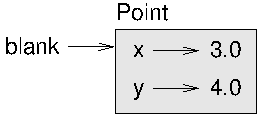
\includegraphics[scale=0.8]{figs/point.pdf}}
\caption{对象图(Object diagram)}
\label{fig.point}
\end{figure}


The variable {\tt blank} refers to a Point object, which
contains two attributes.  Each attribute refers to a
floating-point number.

变量{\tt blank}引用了一个Point类,这个类拥有了两个属性。
每个属性都引用了一个浮点数。

You can read the value of an attribute using the same syntax:

你可以使用相同的语法读出一个属性的值。

\begin{verbatim}
>>> print blank.y
4.0
>>> x = blank.x
>>> print x
3.0
\end{verbatim}
%
The expression {\tt blank.x} means, ``Go to the object {\tt blank}
refers to and get the value of {\tt x}.'' In this case, we assign that
value to a variable named {\tt x}.  There is no conflict between
the variable {\tt x} and the attribute {\tt x}.

表达式{\tt blank.x}的意思是,``前往{\tt blank}所引用的对象并且将{\tt x}的值拿出来''。
在这个例子中,我们将获取到的值赋值给了一个叫做{\tt x}的变量。
变量{\tt x}和属性{\tt x}并不会冲突。

You can use dot notation as part of any expression.  For example:

你可以在任何表达式中使用点号。例如:

\begin{verbatim}
>>> print '(%g, %g)' % (blank.x, blank.y)
(3.0, 4.0)
>>> distance = math.sqrt(blank.x**2 + blank.y**2)
>>> print distance
5.0
\end{verbatim}
%
You can pass an instance as an argument in the usual way.
For example:
\index{instance!as argument}

你可以像往常那样将一个实例作为参数传递。
例如:

\begin{verbatim}
def print_point(p):
    print '(%g, %g)' % (p.x, p.y)
\end{verbatim}
%
\verb"print_point" takes a point as an argument and displays it in
mathematical notation.  To invoke it, you can pass {\tt blank} as
an argument:

\verb"print_point"将一个点作为参数,打印出其在数学中的表示方法。
调用它的时候,你可以将{\tt blank}作为参数传递:

\begin{verbatim}
>>> print_point(blank)
(3.0, 4.0)
\end{verbatim}
%
Inside the function, {\tt p} is an alias for {\tt blank}, so if
the function modifies {\tt p}, {\tt blank} changes.
\index{aliasing}

在这个函数内部,{\tt p}作为{\tt blank}的别名,
所以,当函数修改了{\tt p},{\tt blank}也会随之改变。


\begin{exercise}

Write a function called \verb"distance_between_points" that takes two
Points as arguments and returns the distance between them.

编写一个叫做\verb"distance_between_points"的函数,它将两个Point作为参数,
返回这两个点之间的距离。

\end{exercise}



\section{Rectangles 矩形}
\label{rectangles}

Sometimes it is obvious what the attributes of an object should be,
but other times you have to make decisions.  For example, imagine you
are designing a class to represent rectangles.  What attributes would
you use to specify the location and size of a rectangle?  You can
ignore angle; to keep things simple, assume that the rectangle is
either vertical or horizontal.
\index{representation}

有时候,一个对象该拥有哪些属性是显而易见的,但有时候你需要好好考虑一番。
比如,你需要设计一个代表矩形的类。
为了描述一个矩形的位置和大小,你需要设计哪些属性呢?
角度是可以忽略的;为了使事情更容易,假设矩形是水平放置的。

There are at least two possibilities: 

至少有两种可能的设计:

\begin{itemize}

\item You could specify one corner of the rectangle
(or the center), the width, and the height.

你可以指定矩形的一个角(或是中心),宽度,以及长度。

\item You could specify two opposing corners.

你可以指定对角线上的两个角。

\end{itemize}

At this point it is hard to say whether either is better than
the other, so we'll implement the first one, just as an example.
\index{Rectangle class}
\index{class!Rectangle}

这个时候还不能够说明哪个方法优于哪个方法,为了举例,我们先来实现前者。

Here is the class definition:

这是类的定义:

\begin{verbatim}
class Rectangle(object):
    """Represents a rectangle. 

    attributes: width, height, corner.
    """
\end{verbatim}
%
The docstring lists the attributes:  {\tt width} and
{\tt height} are numbers; {\tt corner} is a Point object that
specifies the lower-left corner.

文档字符串中列出了属性:{\tt width}和{\tt height}是数字;
{\tt corner}是一个Point对象,代表了左下角的那个点。

To represent a rectangle, you have to instantiate a Rectangle
object and assign values to the attributes:

为了描述一个矩形,你需要实例化一个Rectangle对象,并且为它的属性赋值。

\begin{verbatim}
box = Rectangle()
box.width = 100.0
box.height = 200.0
box.corner = Point()
box.corner.x = 0.0
box.corner.y = 0.0
\end{verbatim}
%
The expression {\tt box.corner.x} means,
``Go to the object {\tt box} refers to and select the attribute named
{\tt corner}; then go to that object and select the attribute named
{\tt x}.''

表达式{\tt box.corner.x}的意思是,
``前往{\tt box}所引用的对象,找到叫做{\tt corner}的属性;
然后前往{\tt corner}所引用的对象,找到叫做{\tt x}的属性。

\begin{figure}
\centerline
{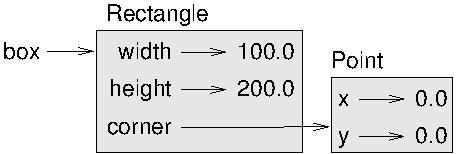
\includegraphics[scale=0.8]{figs/rectangle.pdf}}
\caption{对象图(Object diagram)}
\label{fig.rectangle}
\end{figure}


Figure~\ref{fig.rectangle} shows the state of this object.
\index{state diagram}
\index{diagram!state}
\index{object diagram}
\index{diagram!object}
An object that is an attribute of another object is {\bf embedded}.
\index{embedded object}
\index{object!embedded}

图\ref{fig.rectangle}展示了这个对象的状态。
一个对象作为另一个对象的属性叫做{\bf 嵌套(embedded)}。

\section{Instances as return values 实例作为返回值}
\index{instance!as return value}
\index{return value}

Functions can return instances.  For example, \verb"find_center"
takes a {\tt Rectangle} as an argument and returns a {\tt Point}
that contains the coordinates of the center of the {\tt Rectangle}:

函数可以返回实例。例如,\verb"find_center"将一个{\tt Rectangle}作为参数
返回一个{\tt Point},代表了这个{\tt Rectangle}的中心坐标:

\begin{verbatim}
def find_center(rect):
    p = Point()
    p.x = rect.corner.x + rect.width/2.0
    p.y = rect.corner.y + rect.height/2.0
    return p
\end{verbatim}
%
Here is an example that passes {\tt box} as an argument and assigns
the resulting Point to {\tt center}:

这个例子将{\tt box}作为参数传递,将返回的Point赋值给{\tt center}:

\begin{verbatim}
>>> center = find_center(box)
>>> print_point(center)
(50.0, 100.0)
\end{verbatim}
%

\section{Objects are mutable 对象是可变的}
\index{object!mutable}
\index{mutability}

You can change the state of an object by making an assignment to one of
its attributes.  For example, to change the size of a rectangle
without changing its position, you can modify the values of {\tt
width} and {\tt height}:

你可以通过给一个对象的属性赋值来改变这个对象的状态。
例如,要改变一个矩形的大小而不改变它的位置,你可以修改{\tt width}和{\tt height}的值:

\begin{verbatim}
box.width = box.width + 50
box.height = box.width + 100
\end{verbatim}
%
You can also write functions that modify objects.  For example,
\verb"grow_rectangle" takes a Rectangle object and two numbers,
{\tt dwidth} and {\tt dheight}, and adds the numbers to the
width and height of the rectangle:

你也可以编写函数来修改对象。
例如,\verb"grow_rectangle"接受了一个Rectangle对象和两个数字,
{\tt dwidth}和{\tt dheight},并将其加到矩形的宽度和高度上:

\begin{verbatim}
def grow_rectangle(rect, dwidth, dheight):
    rect.width += dwidth
    rect.height += dheight
\end{verbatim}
%
Here is an example that demonstrates the effect:

这个例子展示了调用后的结果:

\begin{verbatim}
>>> print box.width
100.0
>>> print box.height
200.0
>>> grow_rectangle(box, 50, 100)
>>> print box.width
150.0
>>> print box.height
300.0
\end{verbatim}
%
Inside the function, {\tt rect} is an
alias for {\tt box}, so if the function modifies {\tt rect}, 
{\tt box} changes.

在函数内部,{\tt rect}是{\tt box}的一个别名,
所以如果函数修改了{\tt rect},则{\tt box}也随之改变。

\begin{exercise}

Write a function named \verb"move_rectangle" that takes
a Rectangle and two numbers named {\tt dx} and {\tt dy}.  It
should change the location of the rectangle by adding {\tt dx}
to the {\tt x} coordinate of {\tt corner} and adding {\tt dy}
to the {\tt y} coordinate of {\tt corner}.

编写一个叫做\verb"move_rectangle"的函数,接受一个Rectangle以及两个数字,
{\tt dx}和{\tt dy}。
它把{\tt corner}的{\tt x}坐标加上{\tt dx},把{\tt corner}的{\tt y}坐标加上{\tt dy},
从而改变矩形的位置。


\end{exercise}


\section{Copying 复制}
\label{copying}
\index{aliasing}

Aliasing can make a program difficult to read because changes
in one place might have unexpected effects in another place.
It is hard to keep track of all the variables that might refer
to a given object.
\index{copying objects}
\index{object!copying}
\index{copy module}
\index{module!copy}

别名会造成程序的可读性降低,因为一个地方的变动可能会意外影响另一个地方。
跟踪所有引用同一个对象的变量是非常困难的。

Copying an object is often an alternative to aliasing.
The {\tt copy} module contains a function called {\tt copy} that
can duplicate any object:

通常用复制对象的方法取代为对象起别名。
{\tt copy}模块拥有一个叫做{\tt copy}的函数,可以复制任何对象:

\begin{verbatim}
>>> p1 = Point()
>>> p1.x = 3.0
>>> p1.y = 4.0

>>> import copy
>>> p2 = copy.copy(p1)
\end{verbatim}
%
{\tt p1} and {\tt p2} contain the same data, but they are
not the same Point.

{\tt p1}和{\tt p2}拥有相同的数据,但是它们并不是同一个Point对象。

\begin{verbatim}
>>> print_point(p1)
(3.0, 4.0)
>>> print_point(p2)
(3.0, 4.0)
>>> p1 is p2
False
>>> p1 == p2
False
\end{verbatim}
%
The {\tt is} operator indicates that {\tt p1} and {\tt p2} are not the
same object, which is what we expected.  But you might have expected
{\tt ==} to yield {\tt True} because these points contain the same
data.  In that case, you will be disappointed to learn that for
instances, the default behavior of the {\tt ==} operator is the same
as the {\tt is} operator; it checks object identity, not object
equivalence.  This behavior can be changed---we'll see how later.
\index{is operator}
\index{operator!is}

正如我们预期的,{\tt is}运算符显示了{\tt p1}和{\tt p2}并非同一个对象。
不过你可能会认为{\tt ==}运算的结果应该是{\tt True},因为这两个点的数据是相同的。
然而结果并不如你想象的那样,{\tt ==}运算符的默认行为和{\tt is}运算符相同;
它检查对象的身份是否相同,而非对象的值是否相同。
我们可以改变这个默认的行为---稍后会看到。

If you use {\tt copy.copy} to duplicate a Rectangle, you will find
that it copies the Rectangle object but not the embedded Point.
\index{embedded object!copying}

如果你使用{\tt copy.copy}来复制一个矩形,
你会发现它仅仅复制了Rectangle对象,但没有复制嵌套的Point对象。

\begin{verbatim}
>>> box2 = copy.copy(box)
>>> box2 is box
False
>>> box2.corner is box.corner
True
\end{verbatim}

\begin{figure}
\centerline
{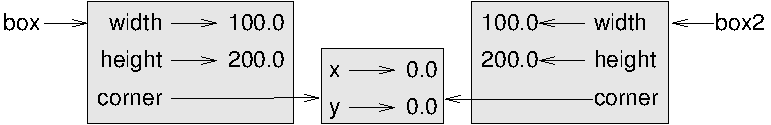
\includegraphics[scale=0.8]{figs/rectangle2.pdf}}
\caption{对象图(Object diagram)}
\label{fig.rectangle2}
\end{figure}

Figure~\ref{fig.rectangle2} shows what the object diagram looks like.
\index{state diagram}
\index{diagram!state}
\index{object diagram}
\index{diagram!object}
This operation is called a {\bf shallow copy} because it copies the
object and any references it contains, but not the embedded objects.
\index{shallow copy}
\index{copy!shallow}

图\ref{fig.rectangle2}展示了这个对象图。
这个操作叫做{\bf 浅复制(shallow copy)},因为仅复制了对象以及其包含的引用,
但未复制嵌套的对象。

For most applications, this is not what you want.  In this example,
invoking \verb"grow_rectangle" on one of the Rectangles would not
affect the other, but invoking \verb"move_rectangle" on either would
affect both!  This behavior is confusing and error-prone.
\index{deep copy}
\index{copy!deep}

对大多数应用来说,这并非是你想要的结果。
在这个例子中,对其中一个Rectangle对象调用\verb"grow_rectangle"并不会影响到另外一个,
然而当对任何一个Rectangle对象调用\verb"move_rectangle"的时候,两者都会被影响!
这个行为很容易带来疑惑和错误。

Fortunately, the {\tt copy} module contains a method named {\tt
deepcopy} that copies not only the object but also 
the objects it refers to, and the objects {\em they} refer to,
and so on.
You will not be surprised to learn that this operation is
called a {\bf deep copy}.
\index{deepcopy function}
\index{function!deepcopy}

幸运的是,{\tt copy}模块拥有一个叫做{\tt deepcopy}的方法,
它不仅可以复制一个对象,还可以复制这个对象所引用的对象,
甚至可以复制{\em 这个对象所引用的对象}所引用的对象,等等。
你应该能明白为什么这个操作叫做{\bf 深复制(deep copy)}了吧。

\begin{verbatim}
>>> box3 = copy.deepcopy(box)
>>> box3 is box
False
>>> box3.corner is box.corner
False
\end{verbatim}
%
{\tt box3} and {\tt box} are completely separate objects.

{\tt box3}和{\tt box}是完全互不相干的对象。

\begin{exercise}

Write a version of \verb"move_rectangle" that creates and
returns a new Rectangle instead of modifying the old one.

编写另一个版本的\verb"move_rectangle",
它创建并返回一个新的Rectangle对象而非修改原先的那个。

\end{exercise}


\section{Debugging 调试}
\label{hasattr}
\index{debugging}

When you start working with objects, you are likely to encounter
some new exceptions.  If you try to access an attribute
that doesn't exist, you get an {\tt AttributeError}:
\index{exception!AttributeError}
\index{AttributeError}

当你开始学习对象的时候,你可能会遇到一些新的异常。
如果你企图使用一个不存在的属性,你会得到{\tt Attributeerror}:

\begin{verbatim}
>>> p = Point()
>>> print p.z
AttributeError: Point instance has no attribute 'z'
\end{verbatim}
%
If you are not sure what type an object is, you can ask:
\index{type function}
\index{function!type}

如果你不确定一个对象的类型,你可以询问:

\begin{verbatim}
>>> type(p)
<type '__main__.Point'>
\end{verbatim}
%
If you are not sure whether an object has a particular attribute,
you can use the built-in function {\tt hasattr}:
\index{hasattr function}
\index{function!hasattr}

如果你不确定一个对象是否拥有某个属性,
你可以使用内置函数{\tt hasattr}:

\begin{verbatim}
>>> hasattr(p, 'x')
True
>>> hasattr(p, 'z')
False
\end{verbatim}
%
The first argument can be any object; the second argument is a {\em
string} that contains the name of the attribute.

第一个参数可以是任何对象;
第二个参数是一个{\em 字符串},代表了某个属性的名字。

\section{Glossary 术语表}

\begin{description}

\item[class(类):] A user-defined type.  A class definition creates a new
class object.
\index{class}

\item[class object(类对象):] An object that contains information about a
user-defined type.  The class object can be used to create instances
of the type.
\index{class object}
\index{object!class}

\item[instance(实例):] An object that belongs to a class.
\index{instance}

\item[attribute(属性):] One of the named values associated with an object.
\index{attribute!instance}
\index{instance attribute}

\item[embedded (object)(嵌套(对象)):] An object that is stored as an attribute
of another object.
\index{embedded object}
\index{object!embedded}

\item[shallow copy(浅复制):] To copy the contents of an object, including
any references to embedded objects;
implemented by the {\tt copy} function in the {\tt copy} module.
\index{shallow copy}

\item[deep copy(深复制):] To copy the contents of an object as well as any
embedded objects, and any objects embedded in them, and so on;
implemented by the {\tt deepcopy} function in the {\tt copy} module.
\index{deep copy}

\item[object diagram(对象图):] A diagram that shows objects, their
attributes, and the values of the attributes.
\index{object diagram}
\index{diagram!object}

\end{description}


\section{Exercises 练习}

\begin{exercise}
\label{canvas}
\index{Swampy}
\index{World module}
\index{module!World}

Swampy (see Chapter~\ref{turtlechap}) provides a module named {\tt
  World}, which defines a user-defined type also called {\tt World}.
You can import it like this:

Swampy(见第\ref{turtlechap}章)提供了一个叫做{\tt World}的模块,
它定义了一个同样叫做{\tt World}的用户自定义类型。
你可以像这样导入它:

\begin{verbatim}
from swampy.World import World
\end{verbatim}

The following code creates a World object and calls
the {\tt mainloop} method, which
waits for the user.

下面的代码创建了一个World对象,
并调用了{\tt mainloop}方法,等待用户的操作。

\begin{verbatim}
world = World()
world.mainloop()
\end{verbatim}

A window should appear with a title bar and an empty square.
We will use this window to draw Points,
Rectangles and other shapes.  
Add the following lines before calling
\verb"mainloop" and run the program again.
\index{Canvas object}
\index{object!Canvas}

应该会出现一个带有标题栏和空白方块的窗口。
我们将会在这个窗口中绘制点、矩形以及其它形状。
在调用\verb"mainloop"之前加入下面这几行代码,并重新运行程序。

\begin{verbatim}
canvas = world.ca(width=500, height=500, background='white')
bbox = [[-150,-100], [150, 100]]
canvas.rectangle(bbox, outline='black', width=2, fill='green4')
\end{verbatim}

You should see a green rectangle with a black outline.
The first line creates a Canvas, which appears in the window
as a white square.  The Canvas object provides methods like
{\tt rectangle} for drawing various shapes.
\index{bounding box}

你会看到一个黑色边框的绿色矩形。
第一行代码创建了一个画布(Canvas),在窗口中以白色方块显示。
画布(Canvas)对象提供了诸如{\tt rectangle}的方法来绘制各种形状。

{\tt bbox} is a list of lists that represents the ``bounding box''
of the rectangle.  The first pair of coordinates is the lower-left
corner of the rectangle; the second pair is the upper-right corner.

{\tt bbox}是列表的列表,代表了矩形的``边界框''。
第一对坐标是矩形的左下角;第二对坐标是矩形的右上角。

You can draw a circle like this:

你可以像这样绘制一个圆:

\begin{verbatim}
canvas.circle([-25,0], 70, outline=None, fill='red')
\end{verbatim}

The first parameter is the coordinate pair for the center of the
circle; the second parameter is the radius.

第一个参数是圆心的坐标;第二个参数是半径。

If you add this line to the program, 
the result should resemble the national flag of Bangladesh
(see \url{http://en.wikipedia.org/wiki/Gallery_of_sovereign-state_flags}).
\index{Bangladesh, national flag}

如果将这行代码加入程序,结果看起来就像是孟加拉国的国旗
(见 \url{http://en.wikipedia.org/wiki/Gallery_of_sovereign-state_flags}))。

\begin{enumerate}

\item Write a function called \verb"draw_rectangle" that takes a
  Canvas and a Rectangle as arguments and draws a
  representation of the Rectangle on the Canvas.

  编写一个叫做\verb"draw_rectangle"的函数,
  接受一个Canvas对象和一个Rectangle对象作为参数,
  并在画布上绘制出这个矩形。

\item Add an attribute named {\tt color} to your Rectangle objects and
  modify \verb"draw_rectangle" so that it uses the color attribute as
  the fill color.

  为你的Rectangle对象添加一个叫做{\tt color}的属性,
  并修改\verb"draw_rectangle"使得可以用color属性作为矩形的填充色。

\item Write a function called \verb"draw_point" that takes a
  Canvas and a Point as arguments and draws a
  representation of the Point on the Canvas.

  编写一个叫做\verb"draw_point"的函数,
  接受一个Canvas对象和一个Point对象作为参数,
  并在画布上绘制出这个点。

\item Define a new class called Circle with appropriate attributes and
  instantiate a few Circle objects.  Write a function called
  \verb"draw_circle" that draws circles on the canvas.
\index{Czech Republic, national flag}

定义一个叫做Circle的新的类,为其添加恰当的属性,并实例化一些Circle对象。
编写一个叫做\verb"draw_circle"的函数在画布上绘制圆。

\item Write a program that draws the national flag of the Czech Republic.
Hint: you can draw a polygon like this:

编写一个程序,绘制出捷克共和国的国旗。
提示:你可以像这样绘制一个多边形:

\begin{verbatim}
points = [[-150,-100], [150, 100], [150, -100]]
canvas.polygon(points, fill='blue')
\end{verbatim}

\end{enumerate}
\index{color list}
\index{available colors}

I have written a small program that lists the available colors;
you can download it from \url{http://thinkpython.com/code/color_list.py}.

我写了一个小程序,可以列出常见的颜色;
你可以在\url{http://thinkpython.com/code/color_list.py}下载到。

\end{exercise}


\chapter{Classes and functions 类和函数}
\label{time}

Code examples from this chapter are available from
\url{http://thinkpython.com/code/Time1.py}.

本章代码可从\url{http://thinkpython.com/code/Time1.py}获取。

\section{Time}
\label{time.object}

As another example of a user-defined type, we'll define a class called
{\tt Time} that records the time of day.  The class definition looks
like this:
\index{user-defined type}
\index{type!user-defined}
\index{Time class}
\index{class!Time}

作为另外一个用户自定义类型的例子,我们将定义一个叫{\tt Time}的类用来记录一天的
时间。类定义如下:

\begin{verbatim}
class Time(object):
    """Represents the time of day.
       
    attributes: hour, minute, second
    """
\end{verbatim}
%
We can create a new {\tt Time} object and assign
attributes for hours, minutes, and seconds:

我们可以创建一个新的{\tt Time}对象然后给hours,minutes,seconds属性赋值:

\begin{verbatim}
time = Time()
time.hour = 11
time.minute = 59
time.second = 30
\end{verbatim}
%
The state diagram for the {\tt Time} object looks like Figure~\ref{fig.time}.
\index{state diagram}
\index{diagram!state}
\index{object diagram}
\index{diagram!object}

{\tt Time}对象的状态图如图~\ref{fig.time}所示。

\begin{exercise}
\label{ex.printtime}

Write a function called \verb"print_time" that takes a 
Time object and prints it in the form {\tt hour:minute:second}.
Hint: the format sequence \verb"'%.2d'" prints an integer using
at least two digits, including a leading zero if necessary.

写一个叫\verb"print_time"的函数,以Time对象作为参数打印出{\tt
hour:minute:second}格式的时间。提示:\verb"'%.2d'"格式化字符串打印出2位有效数字
的整型,如果不足两位用前导0填充。

\end{exercise}

\begin{exercise}
\label{isafter}
\index{boolean function}

Write a boolean function called \verb"is_after" that
takes two Time objects, {\tt t1} and {\tt t2}, and
returns {\tt True} if {\tt t1} follows {\tt t2} chronologically and
{\tt False} otherwise.  Challenge: don't use an {\tt if} statement.

写一个叫\verb"is_after"的布尔函数用两个Time对象作为参数。{\tt t1}和{\tt t2},然
后如果{\tt t1}以时间顺序地在{\tt t2}之后则返回{\tt True}否则返回{\tt False}。挑
战:不要使用{\tt if}语句。
\end{exercise}

\begin{figure}
\centerline
{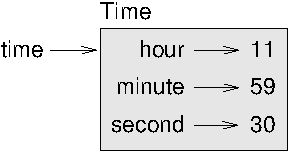
\includegraphics[scale=0.8]{figs/time.pdf}}
\caption{Object diagram.}
\label{fig.time}
\end{figure}


\section{Pure functions 纯函数}
\index{prototype and patch}
\index{development plan!prototype and patch}

In the next few sections, we'll write two functions that add time
values.  They demonstrate two kinds of functions: pure functions and
modifiers.  They also demonstrate a development plan I'll call {\bf
  prototype and patch}, which is a way of tackling a complex problem
by starting with a simple prototype and incrementally dealing with the
complications.

在下面几节中,我们会写两个函数用于增加时间。它们代表了两类函数:纯函数和过程(?)
。它们也是两种开发方式我暂且叫做{\bf 
    %fuzzy%
    原型增量开发
}。是一种以简单原型开始然
后增量式的处理复杂度的方法来解决复杂问题。

Here is a simple prototype of \verb"add_time":

下面是\verb"add_time"的一个简单原型:

\begin{verbatim}
def add_time(t1, t2):
    sum = Time()
    sum.hour = t1.hour + t2.hour
    sum.minute = t1.minute + t2.minute
    sum.second = t1.second + t2.second
    return sum
\end{verbatim}
%
The function creates a new {\tt Time} object, initializes its
attributes, and returns a reference to the new object.  This is called
a {\bf pure function} because it does not modify any of the objects
passed to it as arguments and it has no effect,
like displaying a value or getting user input, 
other than returning a value.
\index{pure function}
\index{function type!pure}

该函数创建一个新的{\tt Time}对象,初始化它的属性,然后返回这个新对象的引用。这
个被叫做{\bf 纯函数}因为它没有修改任何以参数传入的对象并且没有副作用(即打印值
和获得用户输入)。最后返回了一个值\footnote{译注:并且要求不能读写全局变量}。

To test this function, I'll create two Time objects: {\tt start}
contains the start time of a movie, like {\em Monty Python and the
Holy Grail}, and {\tt duration} contains the run time of the movie,
which is one hour 35 minutes.
\index{Monty Python and the Holy Grail}

为了测试这个函数,我会创建两个Time对象:{\tt start}包含一个电影的开始时间,比如
{\em Monty Python and the Holy Grail},然后{\tt duration}包含电影播放的时间,即
1小时35分钟。

\verb"add_time" figures out when the movie will be done.

\verb"add_time"指出了电影什么时候结束。

\begin{verbatim}
>>> start = Time()
>>> start.hour = 9
>>> start.minute = 45
>>> start.second =  0

>>> duration = Time()
>>> duration.hour = 1
>>> duration.minute = 35
>>> duration.second = 0

>>> done = add_time(start, duration)
>>> print_time(done)
10:80:00
\end{verbatim}
%
The result, {\tt 10:80:00} might not be what you were hoping
for.  The problem is that this function does not deal with cases where the
number of seconds or minutes adds up to more than sixty.  When that
happens, we have to ``carry'' the extra seconds into the minute column
or the extra minutes into the hour column.
\index{carrying, addition with}

结果{\tt 10:80:00}可能不是你期待的。问题是这个函数没有处理秒数或分钟数加和超过
60。当它发生了,我们必须``把''额外的秒数进位到分钟或者把额外的分钟进位到小时。

Here's an improved version:

下面是一个增强版:

\begin{verbatim}
def add_time(t1, t2):
    sum = Time()
    sum.hour = t1.hour + t2.hour
    sum.minute = t1.minute + t2.minute
    sum.second = t1.second + t2.second

    if sum.second >= 60:
        sum.second -= 60
        sum.minute += 1

    if sum.minute >= 60:
        sum.minute -= 60
        sum.hour += 1

    return sum
\end{verbatim}
%
Although this function is correct, it is starting to get big.
We will see a shorter alternative later.

虽然这个函数是正确的,但是太繁琐了。我们待会儿重构一个。


\section{Modifiers 过程}
\label{increment}
\index{modifier}
\index{function type!modifier}

Sometimes it is useful for a function to modify the objects it gets as
parameters.  In that case, the changes are visible to the caller.
Functions that work this way are called {\bf modifiers}.
\index{increment}

有时一个函数直接修改传入的参数是非常方便的。在这个时候,改变对于调用者是可见的
。这样的函数叫{\bf 过程}。

{\tt increment}, which adds a given number of seconds to a {\tt Time}
object, can be written naturally as a
modifier.  Here is a rough draft:

{\tt increment},直接对一个{\tt Time}对象增加秒数,可以非常自然地写为过程。下面
是一个粗略的草稿:

\begin{verbatim}
def increment(time, seconds):
    time.second += seconds

    if time.second >= 60:
        time.second -= 60
        time.minute += 1

    if time.minute >= 60:
        time.minute -= 60
        time.hour += 1
\end{verbatim}
%
The first line performs the basic operation; the remainder deals
with the special cases we saw before.
\index{special case}

第一行执行基本的操作;剩下的处理进位问题。

Is this function correct?  What happens if the parameter {\tt seconds}
is much greater than sixty?  

这个函数是正确的吗?如果{\tt seconds}超过60会发生什么?

In that case, it is not enough to carry
once; we have to keep doing it until {\tt time.second} is less than sixty.
One solution is to replace the {\tt if} statements with {\tt while}
statements.  That would make the function correct, but not
very efficient.

这时,进位1次还不够;我们必须循环直到{\tt time.second}小于60。一个解决方案是用
{\tt while}代替{\tt if}语句。那样是正确的,但是不高效。

\begin{exercise}

Write a correct version of {\tt increment} that
doesn't contain any loops.

写一个不包含任何循环的{\tt increment}函数。

\end{exercise}

Anything that can be done with modifiers can also be done with pure
functions.  In fact, some programming languages only allow pure
functions.  There is some evidence that programs that use pure
functions are faster to develop and less error-prone than programs
that use modifiers.  But modifiers are convenient at times,
and functional programs tend to be less efficient.

过程能够做的任何事情纯函数也可以完成。事实上,一些编程语言只支持纯函数
\footnote{译注:一些函数式语言如Haskell,通常认为对高度并发友好}。有一些证据可
以证明使用纯函数的程序比过程式程序开发更快,错误更少。但是有时过程很方便,纯函
数程序开发效率低(?)。

In general, I recommend that you write pure functions whenever it is
reasonable and resort to modifiers only if there is a compelling
advantage.  This approach might be called a {\bf functional
programming style}.
\index{functional programming style}

一般的,我推荐你写纯函数无论是否合理,只有当有巨大的优势时才用过程。这个途径被
成为{\bf 函数式编程}。


\begin{exercise}

Write a ``pure'' version of {\tt increment} that creates and returns
a new Time object rather than modifying the parameter.

写一个``纯''函数版本的{\tt increment}创建返回一个新的Time对象而不是修改它的参数。

\end{exercise}


\section{Prototyping versus planning 原型vs 计划}
\label{prototype}
\index{prototype and patch}
\index{development plan!prototype and patch}
\index{planned development}
\index{development plan!planned}

The development plan I am demonstrating is called ``prototype and
patch.''  For each function, I wrote a prototype that performed the
basic calculation and then tested it, patching errors along the
way.

我描述的被称为``原型增量开发''的开发方法。对于每个函数,我写一个原型执行基本的
计算然后测试它,然后不断的打补丁修正错误。

This approach can be effective, especially if you don't yet have a
deep understanding of the problem.  But incremental corrections can
generate code that is unnecessarily complicated---since it deals with
many special cases---and unreliable---since it is hard to know if you
have found all the errors.

这个方法可以非常高效,特别是当你对问题没有一个深入理解的时候。但是增量式的修正
可能使得代码过度复杂---因为它处理许多特殊的情况---并且不全面---因为它不知道你是
不是找到了所有的错误。

An alternative is {\bf planned development}, in which high-level
insight into the problem can make the programming much easier.  In
this case, the insight is that a Time object is really a three-digit
number in base 60 (see \url{http://en.wikipedia.org/wiki/Sexagesimal}.)!  The
{\tt second} attribute is the ``ones column,'' the {\tt minute}
attribute is the ``sixties column,'' and the {\tt hour} attribute is
the ``thirty-six hundreds column.''
\index{sexagesimal}

一个替代是{\bf 计划开发},就是在一个高层面的对问题的简洁能够使得编程更加容易。
在这里,见解是一个Time对象是一个进位为60的三个数字(参见
\url{http://en.wikipedia.org/wiki/Sexagesimal})!{\tt 秒}属性是
``$\mathbf{1}$'',{\tt 分}属性是``$\mathbf{60}$'',{\tt 时}属性是
``$\mathbf{360}$''。

When we wrote \verb"add_time" and {\tt increment}, we were effectively
doing addition in base 60, which is why we had to carry from one
column to the next.
\index{carrying, addition with}

当我们写\verb"add_time"和{\tt increment},我们实际上用60进制来完成加法,也就是
为什么我们必须从下面进位上来。

This observation suggests another approach to the whole problem---we
can convert Time objects to integers and take advantage of the fact
that the computer knows how to do integer arithmetic.  

观察后了解到另一种解决问题的途径---我们可以可以把Time对象转成一个整型然后利用计
算机知道整型计算这个事实的优势。

Here is a function that converts Times to integers:

下面是把Time转成int的一个函数:

\begin{verbatim}
def time_to_int(time):
    minutes = time.hour * 60 + time.minute
    seconds = minutes * 60 + time.second
    return seconds
\end{verbatim}
%
And here is the function that converts integers to Times
(recall that {\tt divmod} divides the first argument by the second
and returns the quotient and remainder as a tuple).
\index{divmod}

然后下面是一个把int转换为Time的函数(回忆{\tt divmod}用第一个参数除第二个参数然
后返回一个商和余数的元组)。

\begin{verbatim}
def int_to_time(seconds):
    time = Time()
    minutes, time.second = divmod(seconds, 60)
    time.hour, time.minute = divmod(minutes, 60)
    return time
\end{verbatim}
%
You might have to think a bit, and run some tests, to convince
yourself that these functions are correct.  One way to test them is to
check that \verb"time_to_int(int_to_time(x)) == x" for many values of
{\tt x}.  This is an example of a consistency check.
\index{consistency check}

你可以再想想,然后运行测试,使自己确信这个函数是正确的。一个测试它们的方法是检
查\verb"time_to_int(int_to_time(x))==x",{\tt x}取许多值。这个是非常方便的方法
。

Once you are convinced they are correct, you can use them to 
rewrite \verb"add_time":

一旦你确信它们是正确的之后,你可以使用它们来重写\verb"add_time":

\begin{verbatim}
def add_time(t1, t2):
    seconds = time_to_int(t1) + time_to_int(t2)
    return int_to_time(seconds)
\end{verbatim}
%
This version is shorter than the original, and easier to verify.

这个版本比原版更短,而且易于验证。

\begin{exercise}

Rewrite {\tt increment} using \verb"time_to_int" and \verb"int_to_time".

使用\verb"time_to_imt"和\verb"int_to_time"来重写{\tt increment}。

\end{exercise}

In some ways, converting from base 60 to base 10 and back is harder
than just dealing with times.  Base conversion is more abstract; our
intuition for dealing with time values is better.

有时,把60进制转化为10进制或反转比直接处理时间更难。进制转化更加抽象;我们处理
时间的直觉更容易想到。

But if we have the insight to treat times as base 60 numbers and make
the investment of writing the conversion functions (\verb"time_to_int"
and \verb"int_to_time"), we get a program that is shorter, easier to
read and debug, and more reliable.

但是要是我们了解了把时间看作60进制的数然后投入精力完成转化函数
(\verb"time_to_int"和\verb"int_to_time"),我们得到一个更短,更容易读,容易调试,
更可靠的程序。

It is also easier to add features later.  For example, imagine
subtracting two Times to find the duration between them.  The
naive approach would be to implement subtraction with borrowing.
Using the conversion functions would be easier and more likely to be
correct.
\index{subtraction with borrowing}
\index{borrowing, subtraction with}
\index{generalization}

后期加入新特性也非常容易。例如想想用两个时间相减来找到中间的持续时间。朴素的方
式需要实现带借位的减法。使用转换函数会更加容易更加可能正确。

Ironically, sometimes making a problem harder (or more general) makes it
easier (because there are fewer special cases and fewer opportunities
for error).

相反的,有时是一个问题更加困难(或更加一般化)使得它更加简单(因为有更少的特殊
情况就减少错误的可能)。


\section{Debugging 调试}
\index{debugging}

A Time object is well-formed if the values of {\tt minute} and {\tt
second} are between 0 and 60 (including 0 but not 60) and if 
{\tt hour} is positive.  {\tt hour} and {\tt minute} should be
integral values, but we might allow {\tt second} to have a
fraction part.
\index{invariant}

如果Time的{\tt 分钟}和{\tt 秒}是在0到60之间(包括0不包括60)然后{\tt 小时}是正
数。{\tt 小时}和{\tt 分钟}应该是整数,我们让{\tt 秒}可以含有小数部分。满足以上
条件称一个Time对象是合法的。

Requirements like these are called {\bf invariants} because
they should always be true.  To put it a different way, if they
are not true, then something has gone wrong.

像这些需求被称为{\bf 不变条件}因为它们应该总是成立的。如果不是这样的,如果它们
不成立,就会有一些潜在错误。

Writing code to check your invariants can help you detect errors
and find their causes.  For example, you might have a function
like \verb"valid_time" that takes a Time object and returns
{\tt False} if it violates an invariant:

写一个检查你的不变条件的代码能够帮助你检查错误然后发现它们的原因。例如,你可以
写一个叫\verb"valid_time"的函数,以一个Time对象作为参数然后当它不满足不变条件时
返回{\tt False}。

\begin{verbatim}
def valid_time(time):
    if time.hour < 0 or time.minute < 0 or time.second < 0:
        return False
    if time.minute >= 60 or time.second >= 60:
        return False
    return True
\end{verbatim}
%
Then at the beginning of each function you could check the
arguments to make sure they are valid:
\index{raise statement}
\index{statement!raise}

然后在每个函数的开始你应该检查参数保证它们是有效的:

\begin{verbatim}
def add_time(t1, t2):
    if not valid_time(t1) or not valid_time(t2):
        raise ValueError, 'invalid Time object in add_time'
    seconds = time_to_int(t1) + time_to_int(t2)
    return int_to_time(seconds)
\end{verbatim}
%
Or you could use an {\tt assert} statement, which checks a given invariant
and raises an exception if it fails:
\index{assert statement}
\index{statement!assert}

或者你可以使用{\tt assert}语句,检查一个不变条件,当失败是产生一个异常:

\begin{verbatim}
def add_time(t1, t2):
    assert valid_time(t1) and valid_time(t2)
    seconds = time_to_int(t1) + time_to_int(t2)
    return int_to_time(seconds)
\end{verbatim}
%
{\tt assert} statements are useful because they distinguish
code that deals with normal conditions from code
that checks for errors.

{\tt assert}语句是非常有用的因为它们把错误检查代码和处理正确条件的代码区分开来。


\section{Glossary 术语表}

\begin{description}

\item[prototype and patch(原型和增量):] A development plan that involves
writing a rough draft of a program, testing, and correcting errors as
they are found.
\index{prototype and patch}

\item[planned development(计划开发):] A development plan that involves
high-level insight into the problem and more planning than incremental
development or prototype development.
\index{planned development}

\item[pure function(纯函数):] A function that does not modify any of the objects it
receives as arguments.  Most pure functions are fruitful.
\index{pure function}

\item[modifier(过程):] A function that changes one or more of the objects it
receives as arguments.  Most modifiers are fruitless.
\index{modifier}

\item[functional programming style(函数式编程):] A style of program design in which the
majority of functions are pure.
\index{functional programming style}

\item[invariant(不变条件):] A condition that should always be true during the
execution of a program.
\index{invariant}

\end{description}


\section{Exercises 练习}

Code examples from this chapter are available from
\url{http://thinkpython.com/code/Time1.py}; solutions to these
exercises are available from \url{http://thinkpython.com/code/Time1_soln.py}.

本章代码可以从\url{http://thinkpython.com/code/Time1.py}获取;这些练习的答案可
以从\url{http://thinkpython.com/code/Time1_soln.py}获取。

\begin{exercise}

Write a function called \verb"mul_time" that takes a Time object
and a number and returns a new Time object that contains
the product of the original Time and the number.

写一个叫\verb"mul_time"的函数用一个Time对象和一个数字作为参数然后返回一个新的
Time对象,包含原来时间和数字的乘积。

Then use \verb"mul_time" to write a function that takes a Time
object that represents the finishing time in a race, and a number
that represents the distance, and returns a Time object that represents
the average pace (time per mile).
\index{running pace}

然后使用\verb"mul_time"来写一个函数以一个表示一场比赛的结束的时间作为和一个表示
距离的数字作为参数,返回一个表示平均步伐(每英里时间)的时间。

\end{exercise}

%\begin{exercise}
%\index{Date class}
%\index{class!Date}

%Write a class definition for a Date object that has attributes {\tt
%  day}, {\tt month} and {\tt year}.  Write a function called
%\verb"increment_date" that takes a Date object, {\tt date} and an
%integer, {\tt n}, and returns a new Date object that
%represents the day {\tt n} days after {\tt date}.  Hint:
%``Thirty days hath September...''  Challenge: does your function
%deal with leap years correctly?  See \url{http://en.wikipedia.org/wiki/Leap_year}.

%\end{exercise}


\begin{exercise}
\index{datetime module}
\index{module!datetime}

The {\tt datetime} module provides {\tt date} and {\tt time} objects
that are similar to the Date and Time objects in this chapter, but
they provide a rich set of methods and operators.  Read the
documentation at \url{docs.python.org/lib/datetime-date.html}.

{\tt datetime}模块提供了{\tt date}和{\tt time}对象,类似于本章的Date和Time对象
。但是它们提供了一套丰富的方法和运算。阅读
\url{docs.python.org/lib/datetime-date.html}的文档。

\begin{enumerate}

\item Use the {\tt datetime} module to write a program that gets the
  current date and prints the day of the week.
\index{birthday}

使用{\tt datetime}模块来写一个程序,获取当前的日期然后打印星期几。

\item Write a program that takes a birthday as input and prints the
  user's age and the number of days, hours, minutes and seconds until
  their next birthday.

  写一个程序以一个生日作为输入然后打印现在用户的年龄和到下一个生日的天数,小时
  数,分钟数和秒数。

\item For two people born on different days, there is a day when one
  is twice as old as the other. That's their Double Day.  Write a
  program that takes two birthdays and computes their Double Day.

  对于两个生日不同的人,有一天会是一个人是另外一个人年龄的两倍。这叫它们的二重
  日。写一个程序以两个生日作为输入然后计算它们的二重日。

\item For a little more challenge, write the more general version that
  computes the day when one person is $n$ times older than the other.
\index{Double Day}

一个小小的挑战,写一个一般化的程序计算一个人是另外一个人年龄的$n$倍的程序。

\end{enumerate}

\end{exercise}


\chapter{Classes and methods 类和方法}

Code examples from this chapter are available from
\url{http://thinkpython.com/code/Time2.py}.

本章代码可以从\url{http://thinkpython.com/code/Time2.py}获取.

\section{Object-oriented features 面向对象的特性}
\index{object-oriented programming}

Python is an {\bf object-oriented programming language}, which means
that it provides features that support object-oriented
programming.

Python 是一门面向对象语言,意味着它能够支持面向对象编程。

It is not easy to define object-oriented programming, but we have
already seen some of its characteristics:

定义面向对象编程并不容易,但是我们已经见过了它的一些特点:

\begin{itemize}

\item Programs are made up of object definitions and function
definitions, and most of the computation is expressed in terms
of operations on objects.

程序有对象定义和函数定义组成,大多数计算都是在对象上操作的。

\item Each object definition corresponds to some object or concept
in the real world, and the functions that operate on that object
correspond to the ways real-world objects interact.

每个对象定义都是根据一些真实世界的对象或者概念来的,操作对象的函数是根据真实世
界中对象的交互来的。

\end{itemize}

For example, the {\tt Time} class defined in Chapter~\ref{time}
corresponds to the way people record the time of day, and the
functions we defined correspond to the kinds of things people do with
times.  Similarly, the {\tt Point} and {\tt Rectangle} classes
correspond to the mathematical concepts of a point and a rectangle.

例如,在第~\ref{time}章定义的{\tt Time}类是根据人们记录一天的时间来的,我们定义
的函数是根据人们对时间做的一些活动来的。类似的,{\tt Point}和{\tt Rectangle}类
是根据数学概念中的点和矩形来的。

So far, we have not taken advantage of the features Python provides to
support object-oriented programming.  These
features are not strictly necessary; most of them provide
alternative syntax for things we have already done.  But in many cases,
the alternative is more concise and more accurately conveys the
structure of the program.

到现在,我们还没有使用Python提供的面向对象编程特性的优势。这些特性并不是必须的
;它们中大部分是我们已经完成的事情的另外一种语法表达。但是在大多数情况,这些代
替更加简介,更加准确的表达了程序的结构。

For example, in the {\tt Time} program, there is no obvious
connection between the class definition and the function definitions
that follow.  With some examination, it is apparent that every function
takes at least one {\tt Time} object as an argument.
\index{method}
\index{function}

例如,在{\tt Time}程序中,在类定义和接下来的函数定义上并没有明显的联系。仔细观
察的话,每个函数都至少使用一个{\tt Time}对象作为参数。

This observation is the motivation for {\bf methods}; a method is
a function that is associated with a particular class.
We have seen methods for strings, lists, dictionaries and tuples.
In this chapter, we will define methods for user-defined types.
\index{syntax}
\index{semantics}

{\bf 方法}的动机是观测;一个方法是一个和特定的类关联的函数。我们已经看过了字符串,列表,字典和元组的方法。在这章中,我们将会定义用户自定义类型的方法。

Methods are semantically the same as functions, but there are
two syntactic differences:

方法和函数的语义相同,但是有两处句法的不同:

\begin{itemize}

\item Methods are defined inside a class definition in order
to make the relationship between the class and the method explicit.

方法在一个类定义内部声明,为了显示地同类进行关联。

\item The syntax for invoking a method is different from the
syntax for calling a function.

调用方法的语法和调用函数的语法不同。

\end{itemize}

In the next few sections, we will take the functions from the previous
two chapters and transform them into methods.  This transformation is
purely mechanical; you can do it simply by following a sequence of
steps.  If you are comfortable converting from one form to another,
you will be able to choose the best form for whatever you are doing.

在下几节中,我们会把前面两章中的函数转化为方法。这个转化是纯机械式的;你可以通
过以下步骤简单的完成。如果你要想更好的从一种形式转化到另一种形式,你至少需要清
楚的认识到你自己在做什么。


\section{Printing objects 打印对象}
\index{object!printing}

In Chapter~\ref{time}, we defined a class named
{\tt Time} and in Exercise~\ref{ex.printtime}, you 
wrote a function named \verb"print_time":

在第~\ref{time}一章中,我们定义了一个叫{\tt Time}的类,然后在实验
~\ref{ex.printtime}中,你写了一个叫\verb"print_time"的函数:

\begin{verbatim}
class Time(object):
    """Represents the time of day."""

def print_time(time):
    print '%.2d:%.2d:%.2d' % (time.hour, time.minute, time.second)
\end{verbatim}
%
To call this function, you have to pass a {\tt Time} object as an
argument:

为了调用这个函数,你必须把一个{\tt Time}对象作为一个参数传递给函数。

\begin{verbatim}
>>> start = Time()
>>> start.hour = 9
>>> start.minute = 45
>>> start.second = 00
>>> print_time(start)
09:45:00
\end{verbatim}
%
To make \verb"print_time" a method, all we have to do is
move the function definition inside the class definition.  Notice
the change in indentation.
\index{indentation}

为了写一个\verb"print_time"方法,我们需要做的就是在类定义里面定义函数。注意缩进
的变化。

\begin{verbatim}
class Time(object):
    def print_time(time):
        print '%.2d:%.2d:%.2d' % (time.hour, time.minute, time.second)
\end{verbatim}
%
Now there are two ways to call \verb"print_time".  The first
(and less common) way is to use function syntax:
\index{function syntax}
\index{dot notation}

现在有两种方法来调用\verb"print_time"。第一种(也是不常用的)是使用函数的语法:


\begin{verbatim}
>>> Time.print_time(start)
09:45:00
\end{verbatim}
%
In this use of dot notation, {\tt Time} is the name of the class,
and \verb"print_time" is the name of the method.  {\tt start} is
passed as a parameter.

在这个点语法中,{\tt Time}是类的名字,然后\verb"print_time"是方法的名字。{\tt
start}是传递的参数。

The second (and more concise) way is to use method syntax:
\index{method syntax}

第二种语法(也更简洁)是使用方法语法:

\begin{verbatim}
>>> start.print_time()
09:45:00
\end{verbatim}
%
In this use of dot notation, \verb"print_time" is the name of the
method (again), and {\tt start} is the object the method is
invoked on, which is called the {\bf subject}.  Just as the
subject of a sentence is what the sentence is about, the subject
of a method invocation is what the method is about.
\index{subject}

在这个点语法中,\verb"print_time"是方法的名称,然后{\tt start}是调用方法的对象
,被称为主语({\bf subject})。就像一个句子的主语是句子的核心,方法的主语也是方
法作用的主要对象。

Inside the method, the subject is assigned to the first
parameter, so in this case {\tt start} is assigned
to {\tt time}.
\index{self (parameter name)}
\index{parameter!self}

在方法中,主语被赋值为第一个参数,所以在这里{\tt start}被赋值到{\tt time}上了。

By convention, the first parameter of a method is
called {\tt self}, so it would be more common to write
\verb"print_time" like this:

约定方法的第一个参数写作{\tt self},所以可以把\verb"print_time"重新写成:

\begin{verbatim}
class Time(object):
    def print_time(self):
        print '%.2d:%.2d:%.2d' % (self.hour, self.minute, self.second)
\end{verbatim}
%
The reason for this convention is an implicit metaphor:
\index{metaphor, method invocation}

这个约定的原因是一种暗喻。

\begin{itemize}

\item The syntax for a function call, \verb"print_time(start)",
  suggests that the function is the active agent.  It says something
  like, ``Hey \verb"print_time"!  Here's an object for you to print.''

在函数调用的语法中,\verb"print_time(start)"表示函数是一个活跃的代理。就像是在
说``Hi, \verb"print_time"! 这有一个对象要给你去打印''。

\item In object-oriented programming, the objects are the active
  agents.  A method invocation like \verb"start.print_time()" says
  ``Hey {\tt start}!  Please print yourself.''

在面向对象编程中,对象是一个活跃的代理。一个如同\verb"start.print_time()"的方法
调用就像是在说``Hi {\tt start}! 请打印你自己''。

\end{itemize}

This change in perspective might be more polite, but it is not obvious
that it is useful.  In the examples we have seen so far, it may not
be.  But sometimes shifting responsibility from the functions onto the
objects makes it possible to write more versatile functions, and makes
it easier to maintain and reuse code.

视角的转换似乎语气更文雅些了,但没有什么明显的实质的改变。在我们已经看过的例子
中的确如此。但优势从函数上面转移任务到对象上使得更加容易写出万能的函数,并且使
得维护和重用代码更容易。

\begin{exercise}
\label{convert}

Rewrite \verb"time_to_int" (from Section~\ref{prototype}) as a method.
It is probably not appropriate to rewrite \verb"int_to_time" as a
method; what object you would invoke it on?

重写\verb"time_to_int"(第~\ref{prototype}节)作为一个方法。可能把
\verb"int_to_time"重写为一个方法不合适;思考下你应该在哪个对象上调用它?

\end{exercise}


\section{Another example 一个范例}
\index{increment}

Here's a version of {\tt increment} (from Section~\ref{increment})
rewritten as a method:

下面是一个重写为方法的{\tt increment}(来自第~\ref{increment}节)的例子:

\begin{verbatim}
# inside class Time:

    def increment(self, seconds):
        seconds += self.time_to_int()
        return int_to_time(seconds)
\end{verbatim}
%
This version assumes that \verb"time_to_int" is written
as a method, as in Exercise~\ref{convert}.  Also, note that
it is a pure function, not a modifier.

这个版本假设\verb"time_to_int"已经改成了方法了,见练习~\ref{convert}。另外,注
意到这个是一个纯函数。不是一个过程。\footnote{指没有修改自身数据而是返回一个新
的对象}

Here's how you would invoke {\tt increment}:

下面是如何调用{\tt increment}的例子:

\begin{verbatim}
>>> start.print_time()
09:45:00
>>> end = start.increment(1337)
>>> end.print_time()
10:07:17
\end{verbatim}
%
The subject, {\tt start}, gets assigned to the first parameter,
{\tt self}.  The argument, {\tt 1337}, gets assigned to the
second parameter, {\tt seconds}.

{\tt start}主语赋值为第一个参数{\tt self}。{\tt 1337}赋值为第二个参数{\tt
seconds}。

This mechanism can be confusing, especially if you make an error.
For example, if you invoke {\tt increment} with two arguments, you
get:
\index{exception!TypeError}
\index{TypeError}

这个机制可能比较迷惑,特别是当出现了错误。例如,如果你给{\tt increment}两个参数
,你会得到:

\begin{verbatim}
>>> end = start.increment(1337, 460)
TypeError: increment() takes exactly 2 arguments (3 given)
\end{verbatim}
%
The error message is initially confusing, because there are
only two arguments in parentheses.  But the subject is also
considered an argument, so all together that's three.

错误信息则比较迷惑人,因为这里只有2个参数。但是其实主语也算一个参数。所以加起来
一共是三个。

\section{A more complicated example 一个更复杂的例子}

\verb"is_after" (from Exercise~\ref{isafter}) is slightly more complicated
because it takes two Time objects as parameters.  In this case it is
conventional to name the first parameter {\tt self} and the second
parameter {\tt other}:
\index{other (parameter name)}
\index{parameter!other}

\verb"is_after"(来自练习~\ref{isafter})更加复杂一些因为它使用两个Time对象作为
参数。在这里为了方便起见将第一个参数叫做{\tt self}第二个参数叫做{\tt other}:

\begin{verbatim}
# inside class Time:

    def is_after(self, other):
        return self.time_to_int() > other.time_to_int()
\end{verbatim}
%
To use this method, you have to invoke it on one object and pass
the other as an argument:

为了使用这个方法,你必须在一个对象上调用它然后作为参数传递另外一个。

\begin{verbatim}
>>> end.is_after(start)
True
\end{verbatim}
%
One nice thing about this syntax is that it almost reads
like English: ``end is after start?''

一个比较好的事情是这个语法读起来和英语差不多:``end是在start之后吗?''


\section{The init method init方法}
\index{init method}
\index{method!init}

The init method (short for ``initialization'') is
a special method that gets invoked when an object is instantiated.  
Its full name is \verb"__init__" (two underscore characters,
followed by {\tt init}, and then two more underscores).  An
init method for the {\tt Time} class might look like this:

init方法(``initialization''的简称)是一个特殊的方法,当一个对象初始化的时候调
用。它的全名是\verb"__init__"(两个下划线后加{\tt init}再加两个下划线)。一个
{\tt Time}类的init方法看起来像是:

\begin{verbatim}
# inside class Time:

    def __init__(self, hour=0, minute=0, second=0):
        self.hour = hour
        self.minute = minute
        self.second = second
\end{verbatim}
%
It is common for the parameters of \verb"__init__"
to have the same names as the attributes.  The statement

通常\verb"__init__"方法的参数和属性的名称一样。

\begin{verbatim}
        self.hour = hour
\end{verbatim}
%
stores the value of the parameter {\tt hour} as an attribute
of {\tt self}.
\index{optional parameter}
\index{parameter!optional}
\index{default value}
\index{override}

上面的语句把{\tt hour}参数的值储存为{\tt self}的一个属性。

The parameters are optional, so if you call {\tt Time} with
no arguments, you get the default values.

参数是可选的,所以如果你不带参数的调用{\tt Time},你会得到默认值。

\begin{verbatim}
>>> time = Time()
>>> time.print_time()
00:00:00
\end{verbatim}
%
If you provide one argument, it overrides {\tt hour}:

如果你提供一个参数,它会覆盖{\tt hour}:

\begin{verbatim}
>>> time = Time (9)
>>> time.print_time()
09:00:00
\end{verbatim}
%
If you provide two arguments, they override {\tt hour} and
{\tt minute}.

如果你提供两个参数,他们会覆盖{\tt hour}和{\tt minute}。

\begin{verbatim}
>>> time = Time(9, 45)
>>> time.print_time()
09:45:00
\end{verbatim}
%
And if you provide three arguments, they override all three
default values.

如果你提供三个参数,它们会覆盖三个默认值。


\begin{exercise}
\index{Point class}
\index{class!Point}

Write an init method for the {\tt Point} class that takes
{\tt x} and {\tt y} as optional parameters and assigns
them to the corresponding attributes.

为{\tt Point}类写一个init方法,使用{\tt x} 和 {\tt y}作为可选参数然后赋值给对应
的属性。

\end{exercise}


\section{The {\tt \_\_str\_\_} method {\tt \_\_str\_\_}方法}
\index{str method@\_\_str\_\_ method}
\index{method!\_\_str\_\_}

\verb"__str__" is a special method, like \verb"__init__",
that is supposed to return a string representation of an object.
\index{string representation}

\verb"__str__"是一个和\verb"__init__"方法类似的特殊方法,用来返回一个对象的字符
串表达。

For example, here is a {\tt str} method for Time objects:

例如,下面是一个Time对象的{\tt str}方法:

\begin{verbatim}
# inside class Time:

    def __str__(self):
        return '%.2d:%.2d:%.2d' % (self.hour, self.minute, self.second)
\end{verbatim}
%
When you {\tt print} an object, Python invokes the {\tt str} method:
\index{print statement}
\index{statement!print}

当你{\tt print}一个对象,Python调用{\tt str}方法:

\begin{verbatim}
>>> time = Time(9, 45)
>>> print time
09:45:00
\end{verbatim}
%
When I write a new class, I almost always start by writing 
\verb"__init__", which makes it easier to instantiate objects, and 
\verb"__str__", which is useful for debugging.

当我写了一个新的类,我总是从\verb"__init__"开始,使得更容易实例化一个对象,然后
就是\verb"__str__"方法,用于调试。


\begin{exercise}

Write a {\tt str} method for the {\tt Point} class.  Create
a Point object and print it.

写一个{\tt point}类的{\tt str}方法。创建一个Point对象然后打印它。

\end{exercise}


\section{Operator overloading 运算符重载}
\label{operator.overloading}

By defining other special methods, you can specify the behavior
of operators on user-defined types.  For example, if you define
a method named \verb"__add__" for the {\tt Time} class, you can use the
{\tt +} operator on Time objects.

通过定义其它的一些特殊方法,你可以在用户定义的类上指定运算符的行为。例如,如果
你为{\tt Time}类定义了一个叫\verb"__add__"的方法,你可以在Time对象上使用{\tt +}
运算。

Here is what the definition might look like:
\index{add method}
\index{method!add}

下面是定义的例子:

\begin{verbatim}
# inside class Time:

    def __add__(self, other):
        seconds = self.time_to_int() + other.time_to_int()
        return int_to_time(seconds)
\end{verbatim}
%
And here is how you could use it:

然后下面是你应该怎么使用它:

\begin{verbatim}
>>> start = Time(9, 45)
>>> duration = Time(1, 35)
>>> print start + duration
11:20:00
\end{verbatim}
%
When you apply the {\tt +} operator to Time objects, Python invokes
\verb"__add__".  When you print the result, Python invokes 
\verb"__str__".  So there is quite a lot happening behind the scenes!
\index{operator overloading}

当你在Time对象上应用{\tt +}运算符,Python调用\verb"__add__"。当你打印结果,
Python调用\verb"__str__"。所以实际上后台有很多有趣的事情不断的发生!

Changing the behavior of an operator so that it works with
user-defined types is called {\bf operator overloading}.  For every
operator in Python there is a corresponding special method, like 
\verb"__add__".  For more details, see
\url{docs.python.org/ref/specialnames.html}.

改变一个用户自定义类型的运算符的行为被称为{\bf 运算符重载}。对于每一个运算符
Python对应一个特殊的方法,就像\verb"__add__"。更多的对应请参考
\url{docs.python.org/ref/specialnames.html}。

\begin{exercise}

Write an {\tt add} method for the Point class.  

为一个Point类写一个{\tt add}方法。

\end{exercise}


\section{Type-based dispatch 类型分发}

In the previous section we added two Time objects, but you
also might want to add an integer to a Time object.  The
following is a version of \verb"__add__"
that checks the type of {\tt other} and invokes either
\verb"add_time" or {\tt increment}:

在上以节中我们添加了两个Time对象的加法,但是你可能还希望给一个Time对象加一个整数。下面的\verb"__add__"版本检查{\tt other}的类型然后调用\verb"add_time"或者{\tt increment}:

\begin{verbatim}
# inside class Time:

    def __add__(self, other):
        if isinstance(other, Time):
            return self.add_time(other)
        else:
            return self.increment(other)

    def add_time(self, other):
        seconds = self.time_to_int() + other.time_to_int()
        return int_to_time(seconds)

    def increment(self, seconds):
        seconds += self.time_to_int()
        return int_to_time(seconds)
\end{verbatim}
%
The built-in function {\tt isinstance} takes a value and a
class object, and returns {\tt True} if the value is an instance
of the class.
\index{isinstance function}
\index{function!isinstance}

内建的{\tt isinstance}函数使用一个值和一个类对象,如果值是这个类的实例则返回
{\tt True}。

If {\tt other} is a Time object, \verb"__add__" invokes
\verb"add_time".  Otherwise it assumes that the parameter
is a number and invokes {\tt increment}.  This operation is
called a {\bf type-based dispatch} because it dispatches the
computation to different methods based on the type of the
arguments.
\index{type-based dispatch}
\index{dispatch, type-based}

如果{\tt other}是一个Time对象,\verb"__add__"调用\verb"add_time"。否则它假设参
数是一个数字然后调用{\tt increment}。这个操作被称为{\bf 类型分发}。因为它根据参数的
类型来分发不同的计算方法。

Here are examples that use the {\tt +} operator with different
types:

下面是一个在不同类型上使用{\tt +}运算符的例子:

\begin{verbatim}
>>> start = Time(9, 45)
>>> duration = Time(1, 35)
>>> print start + duration
11:20:00
>>> print start + 1337
10:07:17
\end{verbatim}
%
Unfortunately, this implementation of addition is not commutative.
If the integer is the first operand, you get
\index{commutativity}

不幸的是,这个加法的实现没有交换性。如果int是左运算数,你会得到:

\begin{verbatim}
>>> print 1337 + start
TypeError: unsupported operand type(s) for +: 'int' and 'instance'
\end{verbatim}
%
The problem is, instead of asking the Time object to add an integer,
Python is asking an integer to add a Time object, and it doesn't know
how to do that.  But there is a clever solution for this problem: the
special method \verb"__radd__", which stands for ``right-side add.''
This method is invoked when a Time object appears on the right side of
the {\tt +} operator.  Here's the definition:
\index{radd method}
\index{method!radd}

问题在于,Python没有问一个Time对象去加上一个整数,而是问一个int去加上一个Time对
象,然后它不直到该怎么做了。但是这个问题有一个优雅的解决方案:一个特殊的
\verb"__radd__"方法,表示``右手加法''。当一个Time对象在{\tt +}运算符的右手边出
现时调用这个方法。下面是定义:

\begin{verbatim}
# inside class Time:

    def __radd__(self, other):
        return self.__add__(other)
\end{verbatim}
%
And here's how it's used:

然后下面是如何使用:

\begin{verbatim}
>>> print 1337 + start
10:07:17
\end{verbatim}
%

\begin{exercise}

Write an {\tt add} method for Points that works with either a
Point object or a tuple:  

为Point写一个{\tt add}方法,可以对一个Point或是一个元组工作。

\begin{itemize}

\item If the second operand is a Point, the method should return a new
Point whose $x$ coordinate is the sum of the $x$ coordinates of the
operands, and likewise for the $y$ coordinates.

如果右手边是一个Point,方法应该返回一个新的Point,$x$坐标是两个点的$x$的和,$y$
也是一样的。

\item If the second operand is a tuple, the method should add the
first element of the tuple to the $x$ coordinate and the second
element to the $y$ coordinate, and return a new Point with the result. 

如果右手边是一个元组,方法应该让$x$加上元组的第一个元素,$y$加上第二个元素,然
后返回一个新的Point对象。

\end{itemize}

\end{exercise}

\section{Polymorphism 多态}

Type-based dispatch is useful when it is necessary, but (fortunately)
it is not always necessary.  Often you can avoid it by writing functions
that work correctly for arguments with different types.
\index{type-based dispatch}
\index{dispatch!type-based}

类型分发在必要的时候非常有用,但是(比较好的)它不是必须的。通常你可以通过写对
不同的参数类型都适用的函数来避免它。

Many of the functions we wrote for strings will actually
work for any kind of sequence.
For example, in Section~\ref{histogram}
we used {\tt histogram} to count the number of times each letter
appears in a word.

许多我们为字符串写的函数实际上都适用于任何种类的序列。例如在~\ref{histogram}节
中我们适用{\tt histogram}来为每个字母计数:

\begin{verbatim}
def histogram(s):
    d = dict()
    for c in s:
        if c not in d:
            d[c] = 1
        else:
            d[c] = d[c]+1
    return d
\end{verbatim}
%
This function also works for lists, tuples, and even dictionaries,
as long as the elements of {\tt s} are hashable, so they can be used
as keys in {\tt d}.

这个函数也工作于列表,元组,甚至是字典,只要{\tt s}的元素是可哈希的,你就可以把
它用于{\tt d}的键。

\begin{verbatim}
>>> t = ['spam', 'egg', 'spam', 'spam', 'bacon', 'spam']
>>> histogram(t)
{'bacon': 1, 'egg': 1, 'spam': 4}
\end{verbatim}
%
Functions that can work with several types are called {\bf polymorphic}.
Polymorphism can facilitate code reuse.  For example, the built-in
function {\tt sum}, which adds the elements of a sequence, works
as long as the elements of the sequence support addition.
\index{polymorphism}

可以在几个类型上工作的函数叫{\bf 多态}。多态帮助代码复用。例如,内建的{\tt sum}
函数,对一个序列的元素求和,只要元素支持加法就能够工作。

Since Time objects provide an {\tt add} method, they work
with {\tt sum}:

因为Time对象提供了一个{\tt add}方法,它就可以用于{\tt sum}:

\begin{verbatim}
>>> t1 = Time(7, 43)
>>> t2 = Time(7, 41)
>>> t3 = Time(7, 37)
>>> total = sum([t1, t2, t3])
>>> print total
23:01:00
\end{verbatim}
%
In general, if all of the operations inside a function 
work with a given type, then the function works with that type.

通常,如果一个函数内所有的操作都适用于一个类型,那这个函数就能用于该类型。

The best kind of polymorphism is the unintentional kind, where
you discover that a function you already wrote can be
applied to a type you never planned for.

最好的多态是无心成柳柳成荫的,就是你发现你已经写的一个函数在你没有预计的类型上
也能工作的。


\section{Debugging 调试}
\index{debugging}

It is legal to add attributes to objects at any point in the execution
of a program, but if you are a stickler for type theory, it is a
dubious practice to have objects of the same type with different
attribute sets.  It is usually a good idea to
initialize all of an objects attributes in the init method.
\index{init method}
\index{attribute!initializing}

在程序执行的任何地方为一个对象添加属性是合法的,但是如果你是类型理论的拥护者,
那一个相同类型的对象拥有不同的属性集合就会造成混乱。通常是在init方法中初始化好
一个对象的所有属性。

If you are not sure whether an object has a particular attribute, you
can use the built-in function {\tt hasattr} (see Section~\ref{hasattr}).
\index{hasattr function}
\index{function!hasattr}
\index{dict attribute@\_\_dict\_\_ attribute}
\index{attribute!\_\_dict\_\_}

如果你不确定一个对象是否应该有某个属性,你可以适用内建的{\tt hasattr}函数(参见
~\ref{hasattr}节)。

Another way to access the attributes of an object is through the
special attribute \verb"__dict__", which is a dictionary that maps
attribute names (as strings) and values:

另一种访问一个对象的属性的方法是通过特殊的\verb"__dict__"属性,是一个属性名称(
字符串)和值的映射的字典。

\begin{verbatim}
>>> p = Point(3, 4)
>>> print p.__dict__
{'y': 4, 'x': 3}
\end{verbatim}
%
For purposes of debugging, you might find it useful to keep this
function handy:

为了调试目的,你可能发现下面这段代码非常有用:

\begin{verbatim}
def print_attributes(obj):
    for attr in obj.__dict__:
        print attr, getattr(obj, attr)
\end{verbatim}
%
\verb"print_attributes" traverses the items in the object's dictionary
and prints each attribute name and its corresponding value.
\index{traversal!dictionary}
\index{dictionary!traversal}

\verb"print_attributes"遍历一个对象的字典然后打印每个属性的名称和对应的值。

The built-in function {\tt getattr} takes an object and an attribute
name (as a string) and returns the attribute's value.
\index{getattr function}
\index{function!getattr}

内建的{\tt getattr}方法适用一个对象和一个属性名称(字符串)作为参数然后返回属性
的值。


\section{Interface and implementation 接口和实现}

One of the goals of object-oriented design is to make software more
maintainable, which means that you can keep the program working when
other parts of the system change, and modify the program to meet new
requirements.
\index{interface}
\index{implementation}
\index{maintainable}
\index{object-oriented design}

面向对象设计的一个目标是使得软件更容易维护,意味着当系统的其它部分改变的时候或
者是修改程序适应新的需求是,也可以保持程序可运行。

A design principle that helps achieve that goal is to keep
interfaces separate from implementations.  For objects, that means
that the methods a class provides should not depend on how the
attributes are represented.
\index{attribute}

一个使得达到这个目标的设计原则是接口和实现分离。对于对象,就意味着一个类提供的
方法不应该依赖属性的形式。

For example, in this chapter we developed a class that represents
a time of day.  Methods provided by this class include
and \verb"time_to_int", \verb"is_after", and \verb"add_time".

例如,在我们设计的用于表示一天中的时间的类的那一章中。这个类提供的方法包括
\verb"time_to_int",\verb"is_after"和\verb"add_time"。

We could implement those methods in several ways.  The details of the
implementation depend on how we represent time.  In this chapter, the
attributes of a {\tt Time} object are {\tt hour}, {\tt minute}, and
{\tt second}.

我们可以用几种方法来实现这些方法。实现的细节依赖于我们如何表示时间。在这一章中
,{\tt Time}对象的属性是{\tt hour},{\tt minute}和{\tt second}。

As an alternative, we could replace these attributes with
a single integer representing the number of seconds
since midnight.  This implementation would make some methods,
like \verb"is_after", easier to write, but it makes some methods
harder.

另外一种实现,我们可以用单个表示从零点开始的秒数的整型来替代这些属性。这个实现
会使得一些方法,如\verb"is_after"更容易写成,但也使得一些方法更困难。

After you deploy a new class, you might discover a better
implementation.  If other parts of the program are using your
class, it might be time-consuming and error-prone to change the
interface.  

在你完成一个新类是,你可能会发现一个更好的实现。如果其它部分使用了你的类,再来
改变接口则是耗时且易错的。

But if you designed the interface carefully, you can
change the implementation without changing the interface, which
means that other parts of the program don't have to change.

但是如果你小心的设计好接口,你可以改变实现而保持接口不变,这样使得程序的其它部
分不用改变。

Keeping the interface separate from the implementation means that
you have to hide the attributes.  Code in other parts of the program
(outside the class definition) should use methods to read
and modify the state of the object.  They should not access the
attributes directly.  This principle is called {\bf information hiding};
see \url{http://en.wikipedia.org/wiki/Information_hiding}.
\index{information hiding}

保持接口于实现分离意味着你必须隐藏属性。程序其它部分的代码(在类外定义的)应该
使用方法来读取和修改对象的状态。他们不应该直接访问属性。这个原则叫做{\bf 信息隐
藏};参见\url{http://en.wikipedia.org/wiki/Information_hiding}。


\begin{exercise}

Download the code from this chapter
(\url{http://thinkpython.com/code/Time2.py}).  Change the attributes
of {\tt Time} to be a single integer representing seconds since
midnight.  Then modify the methods (and the function
\verb"int_to_time") to work with the new implementation.  You should
not have to modify the test code in {\tt main}.  When you are done,
the output should be the same as before.  Solution:
\url{http://thinkpython.com/code/Time2_soln.py}

下载本章的代码\url{http://thinkpython.com/code/Time2.py}。将{\tt Time}的属性改
成整型,表示零点开始的秒数。然后修改方法(和\verb"int_to_time"函数)适用于新的
实现。你不应该修改在{\tt main}中的测试代码。当你完成了,输出应该是和以前一样的
。答案:\url{http://thinkpython.com/code/Time2_soln.py}。


\end{exercise}


\section{Glossary 术语表}

\begin{description}

\item[object-oriented language(面向对象语言):] A language that provides features,
  such as user-defined classes and method syntax, that facilitate
  object-oriented programming.
\index{object-oriented language}

\item[object-oriented programming(面向对象编程):] A style of programming in which
data and the operations that manipulate it are organized into classes
and methods.
\index{object-oriented programming}

\item[method(方法):] A function that is defined inside a class definition and
is invoked on instances of that class.
\index{method}

\item[subject:] The object a method is invoked on.
\index{subject}

\item[operator overloading(运算符重载):] Changing the behavior of an operator like
{\tt +} so it works with a user-defined type.
\index{overloading}
\index{operator!overloading}

\item[type-based dispatch(类型重载):] A programming pattern that checks the type
of an operand and invokes different functions for different types.
\index{type-based dispatch}

\item[polymorphic(多态):] Pertaining to a function that can work with more
  than one type.  
\index{polymorphism}

\item[information hiding(信息隐藏):] The principle that the interface provided 
by an object should not depend on its implementation, in particular
the representation of its attributes.
\index{information hiding}


\end{description}

\section{Exercises 练习}

\begin{exercise}
\index{default value!avoiding mutable}
\index{mutable object, as default value}
\index{worst bug}
\index{bug!worst}
\index{Kangaroo class}
\index{class!Kangaroo}

This exercise is a cautionary tale about one of the most
common, and difficult to find, errors in Python.
Write a definition for a class named {\tt Kangaroo} with the following
methods:

这个练习是关于Python里面最常见,最难找出来的错误。写一个叫{\tt Kangaroo}的类,
包含以下方法:

\begin{enumerate}

\item An \verb"__init__" method that initializes an attribute named 
\verb"pouch_contents" to an empty list.

一个\verb"__init__"方法初始化一个叫\verb"pounch_contents"的列表为空。

\item A method named \verb"put_in_pouch" that takes an object
of any type and adds it to \verb"pouch_contents".

一个叫\verb"put_in_pounch"的方法将一个任何类型的对象加入\verb"pounch_contents"
。

\item A \verb"__str__" method that returns a string representation
of the Kangaroo object and the contents of the pouch.

一个\verb"__str__"方法返回Kangaroo对象的字符串表达和pounch的内容。

\end{enumerate}
%
Test your code 
by creating two {\tt Kangaroo} objects, assigning them to variables
named {\tt kanga} and {\tt roo}, and then adding {\tt roo} to the
contents of {\tt kanga}'s pouch.

通过创建两个{\tt Kangaroo}对象来测试你的代码,将它们命名为{\tt kanga}和{\tt
roo}。然后将{\tt roo}加入{\tt kanga}的pounch列表。

Download \url{http://thinkpython.com/code/BadKangaroo.py}.  It contains
a solution to the previous problem with one big, nasty bug.
Find and fix the bug.

下载\url{http://thinkpython.com/code/BadKangaroo.py}的代码,它包含上面问题的解
决方案。但是有一个大而丑陋的bug。找出并修正这个bug。

If you get stuck, you can download
\url{http://thinkpython.com/code/GoodKangaroo.py}, which explains the
problem and demonstrates a solution.
\index{aliasing}
\index{embedded object}
\index{object!embedded}

如果你卡住了,你可以下载\url{http://thinkpython.com/code/GoodKangaroo.py}。解释
了这个问题并给出了另一个解答。

\end{exercise}




\begin{exercise}
\index{Visual module}
\index{module!Visual}
\index{vpython module}
\index{module!vpython}

Visual is a Python module that provides 3-D graphics.  It is
not always included in a Python installation, so you might have
to install it from your software repository or, if it's not there,
from \url{vpython.org}.

Visual是Python提供的3-D图形模块。它可能没有包含在Python的标准安装里面。所以你需
要从你的软件源或者从\url{vpython.org}下载。

The following example creates a 3-D space that is 256 units
wide, long and high, and sets the ``center'' to be the
point $(128,128,128)$.  Then it draws a blue sphere.

下面的例子创建了一个256个单位长度的长宽高的3-D空间。然后设置中心在
${128,128,128}$点上。然后它画出一个蓝色球体。

\begin{verbatim}
from visual import *

scene.range = (256, 256, 256)
scene.center = (128, 128, 128)

color = (0.1, 0.1, 0.9)          # mostly blue
sphere(pos=scene.center, radius=128, color=color)
\end{verbatim}

{\tt color} is an RGB tuple; that is, the elements are Red-Green-Blue
levels between 0.0 and 1.0 (see
\url{http://en.wikipedia.org/wiki/RGB_color_model}).

{\tt color}是一个RGB元组,也就是其中的元素是0.0到1.0的红-绿-蓝等级。(参见
\url{http://en.wikipedia.org/wiki/RGB_color_model})。

If you run this code, you should see a window with a black
background and a blue sphere.  If you drag the middle button
up and down, you can zoom in and out.  You can also rotate
the scene by dragging the right button, but with only one
sphere in the world, it is hard to tell the difference.

如果你运行这个代码,你应该看到一个黑色背景的蓝色球体的窗口。如果你按住中建拖动
,你可以放大缩小它。你也可以通过拖动右键来旋转场景。但是因为只有一个球体,你很
难识别场景的变化。

The following loop creates a cube of spheres:

下面的循环创建一个球体的立方:

\begin{verbatim}
t = range(0, 256, 51)
for x in t:
    for y in t:
        for z in t:
            pos = x, y, z
            sphere(pos=pos, radius=10, color=color)
\end{verbatim}

\begin{enumerate}

\item Put this code in a script and make sure it works for
you.

将这个代码粘贴到脚本文件中确保它可以运行。

\item Modify the program so that each sphere in the cube
has the color that corresponds to its position in RGB space.
Notice that the coordinates are in the range 0--255, but
the RGB tuples are in the range 0.0--1.0.
\index{color list}
\index{available colors}

修改程序使得每个立方中的球体都有着它的位置所对应的RGB空间。注意坐标的范围是
0---255,而RGB元组的范围是0.0---1.0。

\item Download \url{http://thinkpython.com/code/color_list.py}
and use the function \verb"read_colors" to generate a list
of the available colors on your system, their names and
RGB values.  For each named color draw a sphere in the
position that corresponds to its RGB values.

下载\url{http://thinkpython.com/code/color_list.py}然后使用其中的
\verb"read_colors"函数来生成一个你系统上可用的颜色的列表,包括它们的名字和RGB值
。在每个颜色的RGB值对应的位置画一个球体。


\end{enumerate}

You can see my solution at \url{http://thinkpython.com/code/color_space.py}.

你可以从\url{http://thinkpython.com/code/color_space.py}看下我的答案。

\end{exercise}


\chapter{Inheritance 继承}

In this chapter I present classes to represent playing cards,
decks of cards, and poker hands.  If you don't play poker, you can
read about it at \url{http://en.wikipedia.org/wiki/Poker}, but you don't have
to; I'll tell you what you need to know for the exercises.
Code examples from this chapter are available from
\url{http://thinkpython.com/code/Card.py}.
\index{playing card, Anglo-American}
\index{card, playing}
\index{poker}

在本章中,我会用类来表示玩纸牌,?decks of cards?,一手牌。如果你不会玩一手牌
,你可以在\url{http://en.wikipedia.org/wiki/Poker}阅读相关规则,但你可以不用,
反正我会告诉你做练习时你需要知道的。这章的代码可以从
\url{http://thinkpython.com/code/Card.py}获取。

If you are not familiar with Anglo-American playing cards,
you can read about them at \url{http://en.wikipedia.org/wiki/Playing_cards}.

如果你不熟悉英美玩法,你可以在\url{http://en.wikipedia.org/wiki/Playing_cards}
了解规则。


\section{Card objects 卡牌对象}

There are fifty-two cards in a deck, each of which belongs to one of
four suits and one of thirteen ranks.  The suits are Spades, Hearts,
Diamonds, and Clubs (in descending order in bridge).  The ranks are
Ace, 2, 3, 4, 5, 6, 7, 8, 9, 10, Jack, Queen, and King.  Depending on
the game that you are playing, an Ace may be higher than King
or lower than 2.
\index{rank}
\index{suit}

一副牌有52张牌,每一张属于4种花色的一个和13个等级的一个。4种花色是黑桃,红心,
方块,梅花(以桥牌中的下降顺序排列)。13个等级是帽,2,3,4,5,6,7,8,9,10,J,Q,K。
根据你玩的游戏的不同,帽可能比K大或者比2小。

If we want to define a new object to represent a playing card, it is
obvious what the attributes should be: {\tt rank} and
{\tt suit}.  It is not as obvious what type the attributes
should be.  One possibility is to use strings containing words like
\verb"'Spade'" for suits and \verb"'Queen'" for ranks.  One problem with
this implementation is that it would not be easy to compare cards to
see which had a higher rank or suit.
\index{encode}
\index{encrypt}
\index{map to}
\index{representation}

如果我们定义一个新的对象来表示玩牌,明显它应该有{\tt rank}和花色({\tt suit})
两个属性。两个属性的类型不太明显。一个可能是使用字符串类型,如包含
\verb"'Spade'"来用于花色或\verb"'Queen'"用于等级。一个问题是这个实现起来不容易
用等级或者花色来比较牌的大小。

An alternative is to use integers to {\bf encode} the ranks and suits.
In this context, ``encode'' means that we are going to define a mapping
between numbers and suits, or between numbers and ranks.  This
kind of encoding is not meant to be a secret (that
would be ``encryption'').

另外一种是使用一个整型来编码等级和花色。在这里,``编码''表示我们要定义一个数字
到花色或数字到等级的字典。这里不是指的``加密''里面的编码。

\newcommand{\mymapsto}{$\mapsto$}

For example, this table shows the suits and the corresponding integer
codes:

例如,下面的表格显示了花色和对应的整数代码:

\begin{tabular}{l c l}
Spades & \mymapsto & 3 \\
Hearts & \mymapsto & 2 \\
Diamonds & \mymapsto & 1 \\
Clubs & \mymapsto & 0
\end{tabular}

This code makes it easy to compare cards; because higher suits map to
higher numbers, we can compare suits by comparing their codes.

这个代码使得比较牌的大小非常容易;因为更高的花色对应更高的数字,我们可以比较数
字来比较花色的的大小。

The mapping for ranks is fairly obvious; each of the numerical ranks
maps to the corresponding integer, and for face cards:

映射等级的大小更加明显;每个数字等级对应这相应的数字,然后对于J,K,Q:

\begin{tabular}{l c l}
Jack & \mymapsto & 11 \\
Queen & \mymapsto & 12 \\
King & \mymapsto & 13 \\
\end{tabular}

I am using the \mymapsto~symbol to make it clear that these mappings
are not part of the Python program.  They are part of the program
design, but they don't appear explicitly in the code.
\index{Card class}
\index{class!Card}

我使用\mymapsto~符号来清楚的表示这些不是Python程序的一部分。它们是程序设计的部分
,但是它们不会出现在代码中。

The class definition for {\tt Card} looks like this:

{\tt Card}类的定义就像下面:

\begin{verbatim}
class Card(object):
    """Represents a standard playing card."""

    def __init__(self, suit=0, rank=2):
        self.suit = suit
        self.rank = rank
\end{verbatim}
%
As usual, the init method takes an optional
parameter for each attribute.  The default card is
the 2 of Clubs.
\index{init method}
\index{method!init}

通常,init 方法为每一个属性选择一个默认值。默认的卡牌是梅花2。

To create a Card, you call {\tt Card} with the
suit and rank of the card you want.

为了创建一张牌,你可以用你需要的花色和等级来调用{\tt Card}。

\begin{verbatim}
queen_of_diamonds = Card(1, 12)
\end{verbatim}
%


\section{Class attributes 类属性}
\label{class.attribute}
\index{class attribute}
\index{attribute!class}

In order to print Card objects in a way that people can easily
read, we need a mapping from the integer codes to the corresponding
ranks and suits.  A natural way to
do that is with lists of strings.  We assign these lists to {\bf class
attributes}:

为了能够以人能够理解的方式来打印卡牌对象,我们需要一个从整数映射到对应的等级和
花色的字符串。一种自然的方法是用字符串列表。我们把这些列表赋值到{\bf 类属性}:

\begin{verbatim}
# inside class Card:

    suit_names = ['Clubs', 'Diamonds', 'Hearts', 'Spades']
    rank_names = [None, 'Ace', '2', '3', '4', '5', '6', '7', 
              '8', '9', '10', 'Jack', 'Queen', 'King']

    def __str__(self):
        return '%s of %s' % (Card.rank_names[self.rank],
                             Card.suit_names[self.suit])
\end{verbatim}
%
Variables like \verb"suit_names" and \verb"rank_names", which are
defined inside a class but outside of any method, are called
class attributes because they are associated with the class object 
{\tt Card}.
\index{instance attribute}
\index{attribute!instance}

\verb"suit_names" 和 \verb"rank_names" 变量定义在一个类的内部但是在方法之外,被
称为类属性。因为他们被关联到{\tt Card}类对象上的。

This term distinguishes them from variables like {\tt suit} and {\tt
  rank}, which are called {\bf instance attributes} because they are
associated with a particular instance.
\index{dot notation}

这个术语将它们同{\tt suit}和{\tt rank}变量区分开来,后者被称为{\bf 实例属性}因
为他们被关联到了特定的实例。

Both kinds of attribute are accessed using dot notation.  For
example, in \verb"__str__", {\tt self} is a Card object,
and {\tt self.rank} is its rank.  Similarly, {\tt Card}
is a class object, and \verb"Card.rank_names" is a
list of strings associated with the class.

这两种属性都使用点符号来访问。例如,在\verb"__str__"中,{\tt self}是一个卡牌对
象,{\tt self.rank}是它的等级。同样的,{\tt Card}是一个类对象,
\verb"Card.rank_names"是一个和类关联的字符串列表。

Every card has its own {\tt suit} and {\tt rank}, but there
is only one copy of \verb"suit_names" and \verb"rank_names".

每一个卡牌都有自己的{\tt suit}和{\tt rank},但是这里只有一份\verb"suit_names"
和\verb"rank_names"拷贝。


Putting it all together, the expression
\verb"Card.rank_names[self.rank]" means ``use the attribute {\tt rank}
from the object {\tt self} as an index into the list \verb"rank_names"
from the class {\tt Card}, and select the appropriate string.''

把这些综合考虑,表达式\verb"Card.rank_names[self.rank]"表示``使用{\tt self}对象
中的{\tt rank}属性作为{\tt Card}类的\verb"rank_names"列表的索引下标,然后获取合
适的字符串。''

The first element of \verb"rank_names" is {\tt None} because there
is no card with rank zero.  By including {\tt None} as a place-keeper,
we get a mapping with the nice property that the index 2 maps to the
string \verb"'2'", and so on.  To avoid this tweak, we could have
used a dictionary instead of a list.

\verb"rank_names"的地一个元素是{\tt None},因为没有卡牌是等级0.通过使用{\tt
None}作为一个占位符,我们可以很好的将索引2映射到字符串\verb"'2'",等等。为了避
免这种技巧,我们也可以使用一个字典来代替列表。

With the methods we have so far, we can create and print cards:

到目前为止我们有的方法,我们可以创建和打印卡牌:

\begin{verbatim}
>>> card1 = Card(2, 11)
>>> print card1
Jack of Hearts
\end{verbatim}

\begin{figure}
\centerline
{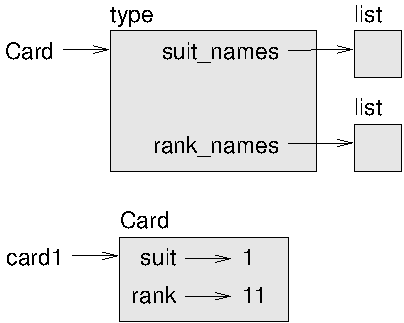
\includegraphics[scale=0.8]{figs/card1.pdf}}
\caption{Object diagram.}
\label{fig.card1}
\end{figure}

Figure~\ref{fig.card1} is a diagram of the {\tt Card} class object
and one Card instance.
\index{state diagram}
\index{diagram!state}
\index{object diagram}
\index{diagram!object}
{\tt Card} is a class object, so it has type {\tt type}.  {\tt
card1} has type {\tt Card}.  (To save space, I didn't draw the
contents of \verb"suit_names" and \verb"rank_names").

图~\ref{fig.card1} 是一个{\tt Card}类对象的图解和一个Card实例。
{\tt Card}是一个类对象,所以它有{\tt type}类型。{\tt card1}有{\tt Card}类型。(
为了节约空间,我没有画出\verb"suit_names" 和 \verb"rank_names")。


\section{Comparing cards 比较大小}
\label{comparecard}
\index{operator!relational}
\index{relational operator}

For built-in types, there are relational operators
({\tt <}, {\tt >}, {\tt ==}, etc.)
that compare
values and determine when one is greater than, less than, or equal to
another.  For user-defined types, we can override the behavior of
the built-in operators by providing a method named
\verb"__cmp__".  

对于内建的类型,有关系运算符({\tt <}, {\tt >}, {\tt ==}, 等等)可以比较值和决定
哪一个是大于,小于或等于另外一个。对于用户定义的类型,我们可以通过提供一个叫
\verb"__cmp__"的方法来覆盖内建的运算符的行为。

\verb"__cmp__" takes two parameters, {\tt self} and {\tt other},
and returns a positive number if the first object is greater, a
negative number if the second object is greater, and 0 if they are
equal to each other.
\index{override}
\index{operator overloading}

\verb"__cmp__" 使用2个参数, {\tt self} 和 {\tt other},如果第一个对象更大,返回
一个正数,第二个元素更大返回一个负数,如果相等返回0.

The correct ordering for cards is not obvious.
For example, which
is better, the 3 of Clubs or the 2 of Diamonds?  One has a higher
rank, but the other has a higher suit.  In order to compare
cards, you have to decide whether rank or suit is more important.

对于卡牌来说正确的顺序不明显。例如,梅花3和方块2哪个更好?一个等级更高,另一个
花色更高。为了比较卡牌,你必须决定等级还是花色更重要。

The answer might depend on what game you are playing, but to keep
things simple, we'll make the arbitrary choice that suit is more
important, so all of the Spades outrank all of the Diamonds,
and so on.
\index{cmp method@\_\_cmp\_\_ method}
\index{method!\_\_cmp\_\_}

答案可能根据你玩的是什么游戏而不同,但是简洁起见,我们规定花色更重要,所以所有
的黑桃大于方块,等等。

With that decided, we can write \verb"__cmp__":

然后,我们可以写\verb"__cmp__"了:

\begin{verbatim}
# inside class Card:

    def __cmp__(self, other):
        # check the suits
        if self.suit > other.suit: return 1
        if self.suit < other.suit: return -1

        # suits are the same... check ranks
        if self.rank > other.rank: return 1
        if self.rank < other.rank: return -1

        # ranks are the same... it's a tie
        return 0    
\end{verbatim}
%
You can write this more concisely using tuple comparison:
\index{tuple!comparison}
\index{comparison!tuple}

你可以使用元组比较来使得代码更加简洁:

\begin{verbatim}
# inside class Card:

    def __cmp__(self, other):
        t1 = self.suit, self.rank
        t2 = other.suit, other.rank
        return cmp(t1, t2)
\end{verbatim}
%
The built-in function {\tt cmp} has the same interface as
the method \verb"__cmp__": it takes two values and returns
a positive number if the first is larger, a negative number
if the second is larger, and 0 if they are equal.
\index{cmp function}
\index{function!cmp}

内建的{\tt cmp}函数的接口和\verb"__cmp__"是一致的:传入2个参数,如果第一个更大
就返回正数,等等。

\begin{exercise}

Write a \verb"__cmp__" method for Time objects.  Hint: you
can use tuple comparison, but you also might consider using
integer subtraction.

为Time对象写一个\verb"__cmp__"方法。要点:你可以使用元组比较,但是你也可以考虑
用整数减法。

%    def __cmp__(self, other):
%        return time_to_int(self) - time_to_int(other)

%If {\tt self} is later than {\tt other}, the result is
%a positive number.  If {\tt other} is later, the result
%is negative.  And if {\tt self} and {\tt other} are equal
%(but not necessarily identical)
%the result is zero.

\end{exercise}


\section{Decks 一副牌}
\index{list!of objects}
\index{deck, playing cards}

Now that we have Cards, the next step is to define Decks.  Since a
deck is made up of cards, it is natural for each Deck to contain a
list of cards as an attribute.
\index{init method}
\index{method!init}

现在我们有Card类了,下一步是定义完整的一副牌了。因为一副牌由许多牌组成,自然地
每一个Deck都有一个卡牌列表作为属性。

The following is a class definition for {\tt Deck}.  The
init method creates the attribute {\tt cards} and generates
the standard set of fifty-two cards:
\index{composition}
\index{loop!nested}
\index{Deck class}
\index{class!Deck}

下面是一个{\tt Deck}的类定义。初始化方法创建了{\tt cards}属性然后生成了一套标准
的52张牌。

\begin{verbatim}
class Deck(object):

    def __init__(self):
        self.cards = []
        for suit in range(4):
            for rank in range(1, 14):
                card = Card(suit, rank)
                self.cards.append(card)
\end{verbatim}
%
The easiest way to populate the deck is with a nested loop.  The outer
loop enumerates the suits from 0 to 3.  The inner loop enumerates the
ranks from 1 to 13.  Each iteration
creates a new Card with the current suit and rank,
and appends it to {\tt self.cards}.
\index{append method}
\index{method!append}

生成一副牌的最简单方法是使用嵌套循环。外层循环枚举0到3的花色。内层循环枚举1到13
的等级。每一个迭代都用当前的花色和等级创建一张新的牌。然后放入{\tt self.cards}
中。


\section{Printing the deck 打印一副牌}
\label{printdeck}
\index{str method@\_\_str\_\_ method}
\index{method!\_\_str\_\_}

Here is a \verb"__str__" method for {\tt Deck}:

{\tt Deck}有一个 \verb"__str__" 方法:

\begin{verbatim}
#inside class Deck:

    def __str__(self):
        res = []
        for card in self.cards:
            res.append(str(card))
        return '\n'.join(res)
\end{verbatim}
%
This method demonstrates an efficient way to accumulate a large
string: building a list of strings and then using {\tt join}.
The built-in function {\tt str} invokes the \verb"__str__"
method on each card and returns the string representation.
\index{accumulator!string}
\index{string!accumulator}
\index{join method}
\index{method!join}
\index{newline}

这个方法展示了积累大字符串的高效方法:建立一个字符串列表然后使用{\tt join}。
内建的{\tt str}函数调用\verb"__str__"方法。在每个卡牌上调用就会返回它们的字符串
表示。

Since we invoke {\tt join} on a newline character, the cards
are separated by newlines.  Here's what the result looks like:

因为我们在新的一行调用的{\tt join},所以卡牌用回车分隔,下面是一个结果示例:

\begin{verbatim}
>>> deck = Deck()
>>> print deck
Ace of Clubs
2 of Clubs
3 of Clubs
...
10 of Spades
Jack of Spades
Queen of Spades
King of Spades
\end{verbatim}
%
Even though the result appears on 52 lines, it is
one long string that contains newlines.

虽然这个结果有52行,但他实际上是包含回车符的一个大字符串。


\section{Add, remove, shuffle and sort 添加,移除,洗牌和排序}

To deal cards, we would like a method that
removes a card from the deck and returns it.
The list method {\tt pop} provides a convenient way to do that:
\index{pop method}
\index{method!pop}

为了发牌,我们需要一个可以把卡牌从一副牌中移除并返回的方法。
列表的{\tt pop}方法提供了一个方便的方式来完成:

\begin{verbatim}
#inside class Deck:

    def pop_card(self):
        return self.cards.pop()
\end{verbatim}
%
Since {\tt pop} removes the {\em last} card in the list, we are
dealing from the bottom of the deck.  In real life ``bottom dealing'' is
frowned upon,
but in this context it's ok.
\index{append method}
\index{method!append}
因为{\tt pop} 移除列表的最后一张卡牌,所以我们我们从底下发牌。在真实环境中``底
部发牌''不太好,但是这里没有关系。

To add a card, we can use the list method {\tt append}:

为了添加一张卡牌,我们使用列表的{\tt append}方法:

\begin{verbatim}
#inside class Deck:

    def add_card(self, card):
        self.cards.append(card)
\end{verbatim}
%
A method like this that uses another function without doing
much real work is sometimes called a {\bf veneer}.  The metaphor
comes from woodworking, where it is common to glue a thin
layer of good quality wood to the surface of a cheaper piece of
wood.
\index{veneer}

像这样使用另外一个函数因此不用做太多工作的方法有时被称为{\bf veneer}。这个隐喻
来源于木工活,通常用一片高质量的木质薄层粘贴在一块便宜木材的表面。

In this case we are defining a ``thin'' method that expresses
a list operation in terms that are appropriate for decks.

在这里,我们定义了一个表示在玩牌的术语中合适的列表操作的``瘦''方法。

As another example, we can write a Deck method named {\tt shuffle}
using the function {\tt shuffle} from the {\tt random} module:
\index{random module}
\index{module!random}
\index{shuffle function}
\index{function!shuffle}

另外一个例子,我们可以给Deck写一个叫{\tt shuffle}的方法,用{\tt random}模块中的
{\tt shuffle}函数。

\begin{verbatim}
# inside class Deck:
            
    def shuffle(self):
        random.shuffle(self.cards)
\end{verbatim}
%
Don't forget to import {\tt random}.

最后不要忘记了导入{\tt random}。

\begin{exercise}
\index{sort method}
\index{method!sort}

Write a Deck method named {\tt sort} that uses the list method
{\tt sort} to sort the cards in a {\tt Deck}.  {\tt sort} uses
the \verb"__cmp__" method we defined to determine sort order.
\end{exercise}

用列表的{\tt sort}方法来写一个Deck的{\tt sort}方法。用于在{\tt Deck}中排序。
{\tt sort}使用我们定义的\verb"__cmp__"来决定排序顺序。



\section{Inheritance 继承}
\index{inheritance}
\index{object-oriented programming}

The language feature most often associated with object-oriented
programming is {\bf inheritance}.  Inheritance is the ability to
define a new class that is a modified version of an existing
class.
\index{parent class}
\index{child class}
\index{class!child}
\index{subclass}
\index{superclass}

和面向对象编程联系最紧密的语言特性就是继承了。基层是在一个已经存在的类的基础上
定义出来的经过一些修改的新的类的能力。

It is called ``inheritance'' because the new class inherits the
methods of the existing class.  Extending this metaphor, the existing
class is called the {\bf parent} and the new class is
called the {\bf child}.

它之所以被称为``继承''是因为新的类从旧的类中继承了方法。由此,已经存在的类被称
为父类,新的类被称为子类。

As an example, let's say we want a class to represent a ``hand,''
that is, the set of cards held by one player.  A hand is similar to a
deck: both are made up of a set of cards, and both require operations
like adding and removing cards.

例如,我们想用一个类来表示一只``手''。也就是,被一个玩家持有的卡牌的集合。手上
的牌(hand)和整副牌(deck)类似:都是由一个卡牌的集合组成,都要求添加和移除卡牌的
动作。

A hand is also different from a deck; there are operations we want for
hands that don't make sense for a deck.  For example, in poker we
might compare two hands to see which one wins.  In bridge, we might
compute a score for a hand in order to make a bid.

hand也和deck不同;有些方法我们希望hand有而deck没有。例如,在扑克牌中我们也许可
以比较两手牌来看哪边赢了。在桥牌中,我们可以计算一手牌的得分来完成一个赌约。

This relationship between classes---similar, but different---lends
itself to inheritance.  

这两个类的关系---有些相似,但又不同---就可以尝试使用继承了。

The definition of a child class is like other class definitions,
but the name of the parent class appears in parentheses:
\index{parentheses!parent class in}
\index{parent class}
\index{class!parent}
\index{Hand class}
\index{class!Hand}

定义一个子类的方式和定义一个普通类比较相似,但是需要在括号写是父类的名称:

\begin{verbatim}
class Hand(Deck):
    """Represents a hand of playing cards."""
\end{verbatim}
%
This definition indicates that {\tt Hand} inherits from {\tt Deck};
that means we can use methods like \verb"pop_card" and \verb"add_card"
for Hands as well as Decks.

这个定义表示了{\tt Hand}继承自{\tt Deck};也就是我们也可以对Hands使用Deck的
\verb"pop_card" 和 \verb"add_card"方法。

{\tt Hand} also inherits \verb"__init__" from {\tt Deck}, but
it doesn't really do what we want: instead of populating the hand
with 52 new cards, the init method for Hands should initialize
{\tt cards} with an empty list.
\index{override}
\index{init method}
\index{method!init}

{\tt Hand}也继承{\tt Deck}的\verb"__init__"方法,但是它并不做我们想做的:不要给
hand生成52张牌,而是为Hands初始化一个空的{\tt cards}列表。

If we provide an init method in the {\tt Hand} class, it overrides the
one in the {\tt Deck} class:

如果我们提供一个{\tt Hand}的init方法,它会覆盖{\tt Deck}类继承来的。

\begin{verbatim}
# inside class Hand:

    def __init__(self, label=''):
        self.cards = []
        self.label = label
\end{verbatim}
%
So when you create a Hand, Python invokes this init method:

所以当你创建了一个Hand,Python会调用这个init方法:

\begin{verbatim}
>>> hand = Hand('new hand')
>>> print hand.cards
[]
>>> print hand.label
new hand
\end{verbatim}
%
But the other methods are inherited from {\tt Deck}, so we can use
\verb"pop_card" and \verb"add_card" to deal a card:

但是其它方法可以从{\tt Deck}继承,所以我们可以使用\verb"pop_card" 和
\verb"add_card"来处理卡牌:

\begin{verbatim}
>>> deck = Deck()
>>> card = deck.pop_card()
>>> hand.add_card(card)
>>> print hand
King of Spades
\end{verbatim}
%
A natural next step is to encapsulate this code in a method
called \verb"move_cards":
\index{encapsulation}

很自然的,可以把这些代码封装成一个\verb"move_cards"的方法:

\begin{verbatim}
#inside class Deck:

    def move_cards(self, hand, num):
        for i in range(num):
            hand.add_card(self.pop_card())
\end{verbatim}
%
\verb"move_cards" takes two arguments, a Hand object and the number of
cards to deal.  It modifies both {\tt self} and {\tt hand}, and
returns {\tt None}.

\verb"move_cards" 有两个参数,一个是Hand对象,另外一个是处理的卡牌的数量。它会
同时修改{\tt self}和{\tt hand},然后返回{\tt None}。

In some games, cards are moved from one hand to another,
or from a hand back to the deck.  You can use \verb"move_cards"
for any of these operations: {\tt self} can be either a Deck
or a Hand, and {\tt hand}, despite the name, can also be a {\tt Deck}.

在有些游戏里面,卡牌从一只手移动到另外一只手,或者从手退还到牌堆里面。你可以在
这几个动作中都使用 \verb"move_cards":{\tt self}可以是一个Deck或者一个Hand,并
且不要管{\tt hand}这个名字的话,它也可以是一个{\tt Deck}。

\begin{exercise}

Write a Deck method called \verb"deal_hands" that takes two
parameters, the number of hands and the number of cards per
hand, and that creates new Hand objects, deals the appropriate
number of cards per hand, and returns a list of Hand objects.

为Deck写一个叫\verb"deal_hands"的方法,使用两个参数,hand的数量的每个hand中card
的数量,然后创建许多新的Hand对象,分给每个hand合适数量的卡牌,然后返回这些Hand
对象的列表。

\end{exercise}

Inheritance is a useful feature.  Some programs that would be
repetitive without inheritance can be written more elegantly
with it.  Inheritance can facilitate code reuse, since you can
customize the behavior of parent classes without having to modify
them.  In some cases, the inheritance structure reflects the natural
structure of the problem, which makes the program easier to
understand.

继承是一个非常有用的特性。有了继承,一些重复性的代码可以写得非常的优雅。继承能
够帮助代码重用,因为你可以自定义父类而不用修改它们\footnote{通过自定义父类成为
子类,使用子类的同时不必修改父类的代码}。在一些案例中,继承的结构反映了真实问题
的结构,使得程序更易于理解。

On the other hand, inheritance can make programs difficult to read.
When a method is invoked, it is sometimes not clear where to find its
definition.  The relevant code may be scattered among several modules.
Also, many of the things that can be done using inheritance can be
done as well or better without it.  

另一方面,继承又可能会使得程序更加难读。当调用了一个方法,有时候搞不清楚调用的
是父类的还是子类的。相关的代码肯能被分散在几个模块之中。并且用继承完成的许多事
情也可以不用继承来完成,而且完成得更好。


\section{Class diagrams 类图}
\label{class.diagram}

So far we have seen stack diagrams, which show the state of
a program, and object diagrams, which show the attributes
of an object and their values.  These diagrams represent a snapshot
in the execution of a program, so they change as the program
runs.

到目前为止我们已经看过了栈图了,显示了一个程序和一个对象的状态的图,或者显示一
个对象的属性和它们的值的图。这些图表达了程序执行的一个快照,所以它们随着程序的
运行而改变。

They are also highly detailed; for some purposes, too
detailed.  A class diagram is a more abstract representation
of the structure of a program.  Instead of showing individual
objects, it shows classes and the relationships between them.

它们也十分的详细;但有一些时候显得过于详细了。一个类图是一个程序的结构的抽象表
达。它显示类和类之间的关系而不是每个独立的对象。

There are several kinds of relationship between classes:

类之间有如下几种关系:

\begin{itemize}

\item Objects in one class might contain references to objects
in another class.  For example, each Rectangle contains a reference
to a Point, and each Deck contains references to many Cards.
This kind of relationship is called {\bf HAS-A}, as in, ``a Rectangle
has a Point.''

一个类中的对象可以包含另外一个类的对象的引用。例如,每一个矩形包含点的引用,每
一个Deck包含许多的Card。这种关系被称为组合({\bf HAS-A}),例如:``一个矩形有一个
点''

\item One class might inherit from another.  This relationship
is called {\bf IS-A}, as in, ``a Hand is a kind of a Deck.''

一个类可能继承于另外一个类。这种关系被称为继承({\bf IS-A}),例如:``一个Hand继承
自Deck''。

\item One class might depend on another in the sense that changes
in one class would require changes in the other.

一个类可能强烈依赖于另一个类,改变一个类就必须改变另一个。

\end{itemize}
\index{IS-A relationship}
\index{HAS-A relationship}
\index{class diagram}
\index{diagram!class}

A {\bf class diagram} is a graphical representation of these
relationships.  For example, Figure~\ref{fig.class1} shows the
relationships between {\tt Card}, {\tt Deck} and {\tt Hand}.

一个类图是这些关系的图形化表示。例如,图~\ref{fig.class}显示了{\tt Card}, {\tt
Deck} 和 {\tt Hand}的关系。

\begin{figure}
\centerline
{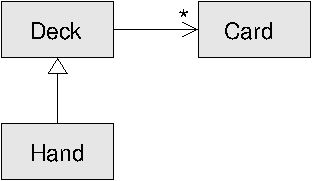
\includegraphics[scale=0.8]{figs/class1.pdf}}
\caption{Class diagram.}
\label{fig.class1}
\end{figure}


The arrow with a hollow triangle head represents an IS-A
relationship; in this case it indicates that Hand inherits
from Deck.

带空心三角的箭头表示一个IS-A的关系;在这种条件下它表示Hand继承自Deck。

The standard arrow head represents a HAS-A
relationship; in this case a Deck has references to Card
objects.
\index{multiplicity (in class diagram)}

标准箭头表示一个HAS-A关系;这里表示一个Deck有Card对象的引用。

The star ({\tt *}) near the arrow head is a 
{\bf multiplicity}; it indicates how many Cards a Deck has.
A multiplicity can be a simple number, like {\tt 52}, a range,
like {\tt 5..7} or a star, which indicates that a Deck can
have any number of Cards.

在箭头旁边的星({\tt *})是一个复数表达;它表示一个Deck有许多Card。一个复数表达
也可以是一个简单的数字(如{\tt 52}),一个范围(如{\tt 5..7})或者是*,表示有任意
数量的Card。

A more detailed diagram might show that a Deck actually
contains a {\em list} of Cards, but built-in types
like list and dict are usually not included in class diagrams.

更详细的图可以显示一个Deck实际上包含一个Card的列表,但是在类图中不包含如list和
dict等的内建内型。

\begin{exercise}

Read {\tt TurtleWorld.py}, {\tt World.py} and {\tt Gui.py}
and draw a class diagram that shows the relationships among
the classes defined there.

阅读 {\tt TurtleWorld.py}, {\tt World.py} 和 {\tt Gui.py}然后画出在文件中定义的
类的类图,包含类之间的关系。

\end{exercise}


\section{Debugging 调试}
\index{debugging}

Inheritance can make debugging a challenge because when you
invoke a method on an object, you might not know which method
will be invoked.
\index{polymorphism}

继承会使得调试变得更加复杂,因为你可能不知道实际调用的是哪个类的方法。

Suppose you are writing a function that works with Hand objects.
You would like it to work with all kinds of Hands, like
PokerHands, BridgeHands, etc.  If you invoke a method like
{\tt shuffle}, you might get the one defined in {\tt Deck},
but if any of the subclasses override this method, you'll
get that version instead.  
\index{flow of execution}

假设你写了一个处理Hand对象的函数。你可能会想让它可以处理所有种类的Hand,如
PockerHand,BridgeHand等等。如果你调用如{\tt shuffle}的方法,你可能会得到在{\tt
Deck}中的那个,但是如果有任何一个子类覆盖了这个方法。你实际上得到的是子类的那个
。

Any time you are unsure about the flow of execution through your
program, the simplest solution is to add print statements at the
beginning of the relevant methods.  If {\tt Deck.shuffle} prints a
message that says something like {\tt Running Deck.shuffle}, then as
the program runs it traces the flow of execution.

任何时候你只要不确定程序的执行流程,最简单的方法是在相关方法的开始处添加print语
句。如果{\tt Deck.shuffle}打印一条如像{\tt Running Deck.shuffle}的消息,通过这
样就可以追踪程序的执行流程。

As an alternative, you could use this function, which takes an
object and a method name (as a string) and returns the class that
provides the definition of the method:

另外一种方法,你可以使用下面的函数,以一个对象和一个方法的名字(字符串格式)作
为参数,然后返回提供这个方法定义的类:

\begin{verbatim}
def find_defining_class(obj, meth_name):
    for ty in type(obj).mro():
        if meth_name in ty.__dict__:
            return ty
\end{verbatim}
%
Here's an example:

下面是一个例子:

\begin{verbatim}
>>> hand = Hand()
>>> print find_defining_class(hand, 'shuffle')
<class 'Card.Deck'>
\end{verbatim}
%
So the {\tt shuffle} method for this Hand is the one in {\tt Deck}.
\index{mro method}
\index{method!mro}
\index{method resolution order}

所以Hand的 {\tt shuffle} 方法是来自于 {\tt Deck}的。

\verb"find_defining_class" uses the {\tt mro} method to get the list
of class objects (types) that will be searched for methods.  ``MRO''
stands for ``method resolution order.''
\index{override}
\index{interface}
\index{precondition}
\index{postcondition}

\verb"find_defining_class"用{\tt mor}方法来获得将类对象的列表,系统将会从这里依
次搜索哪个类提供了这个方法。``MOR''表示``method resolution order''。

Here's a program design suggestion: whenever you override a method,
the interface of the new method should be the same as the old.  It
should take the same parameters, return the same type, and obey the
same preconditions and postconditions.  If you obey this rule, you
will find that any function designed to work with an instance of a
superclass, like a Deck, will also work with instances of subclasses
like a Hand or PokerHand.

对于程序设计的一个建议:无论什么时候你打算覆盖一个方法,新方法的声明必须和旧的
保持一致。它们应该使用相同的参数,返回相同的类型,遵守相同的先决条件和后置条件
。如果你遵守这个规定,你可以发现你设计的任何函数,只要能工作于一个父类的对象(
如Deck),就能够工作于任何子类的对象(如Hand和PockerHand)。

If you violate this rule, your code will collapse like (sorry)
a house of cards.

如果你违背这条规则,你的代码逻辑就会被搞的乱七八糟的。


\section{Data encapsulation 数据封装}

Chapter~\ref{time} demonstrates a development plan we might call
``object-oriented design.''  We identified objects we needed---{\tt
  Time}, {\tt Point} and {\tt Rectangle}---and defined classes to
represent them.  In each case there is an obvious correspondence
between the object and some entity in the real world (or at least a
mathematical world).
\index{development plan}

第~\ref{time}章描述了我们称之为``面向对象设计''的开发计划。我们选择我们需要的对
象---{\tt Time},{\tt Point}和{\tt Rectangle}---然后定义代表它们的类。每种情况都
有一个在对象和真实世界(或至少是在数学世界中)的实例的明显的对应关系。

But sometimes it is less obvious what objects you need
and how they should interact.  In that case you need a different
development plan.  In the same way that we discovered function
interfaces by encapsulation and generalization, we can discover
class interfaces by {\bf data encapsulation}.
\index{data encapsulation}
\index{encapsulation!data}

但是有时有很难界定你需要的对象和设计它们的交互。在这个时候,你需要一个不同的开
发计划。同样的,我们通过封装和组织来探索函数的接口,我们也可以通过数据封装来探
索类的接口。

Markov analysis, from Section~\ref{markov}, provides a good example.
If you download my code from \url{http://thinkpython.com/code/markov.py},
you'll see that it uses two global variables---\verb"suffix_map" and
\verb"prefix"---that are read and written from several functions.

第~\ref{markov}节的马尔科夫设计提供了一个很好的例子。如果你从
\url{http://thinkpython.com/code/markov.py}下载我的代码,你可以看到它使用两个全
局变量---\verb"suffix_map"和\verb"prefix"。用一些函数读写它们的设计思想。


\begin{verbatim}
suffix_map = {}        
prefix = ()            
\end{verbatim}

Because these variables are global
we can only run one analysis
at a time.  If we read two texts, their prefixes and suffixes would
be added to the same data structures (which makes for some interesting
generated text).

因为这些变量是全局的,我们一次只能运行一个分析。如果我们读取了两个文本,它们的
前缀和后缀会被加入相同的数据结构(会使得输出文本混乱)。

To run multiple analyses, and keep them separate, we can encapsulate
the state of each analysis in an object.
Here's what that looks like:

为了同时运行多个分析,并且保持它们的相互独立,我们可以把每个分析的状态封装到一
个对象中。下面是一个例子:

\begin{verbatim}
class Markov(object):

    def __init__(self):
        self.suffix_map = {}
        self.prefix = ()    
\end{verbatim}

Next, we transform the functions into methods.  For example,
here's \verb"process_word":

下一步,我们把这些函数转换为方法。例如:下面是\verb"process_word":

\begin{verbatim}
    def process_word(self, word, order=2):
        if len(self.prefix) < order:
            self.prefix += (word,)
            return

        try:
            self.suffix_map[self.prefix].append(word)
        except KeyError:
            # if there is no entry for this prefix, make one
            self.suffix_map[self.prefix] = [word]

        self.prefix = shift(self.prefix, word)        
\end{verbatim}

Transforming a program like this---changing the design without
changing the function---is another example of refactoring
(see Section~\ref{refactoring}).
\index{refactoring}

像这样转换一个程序---改变设计而保持功能不变---是另外一种重构的例子(参见第
~\ref{refactoring}节)。

This example suggests a development plan for designing objects and
methods:

下面的例子给出了一些设计对象和方法的建议。

\begin{enumerate}

\item Start by writing functions that read and write global
variables (when necessary).

首先从读写全局变量的函数开始(如有必要)。

\item Once you get the program working, look for associations
between global variables and the functions that use them.

一旦你让程序跑起来了,看和全局变量和使用它们的函数的联系。

\item Encapsulate related variables as attributes of an object.

封装相关的变量作为一个对象的属性。

\item Transform the associated functions into methods of the new
class.

转换相关联的函数为新类的方法。

\end{enumerate}


\begin{exercise}

Download my code from Section~\ref{markov}
(\url{http://thinkpython.com/code/markov.py}), and follow the steps described
above to encapsulate the global variables as attributes of a new class
called {\tt Markov}.  Solution: \url{http://thinkpython.com/code/Markov.py}
(note the capital M).

从~\ref{markov}(\url{http://thinkpython.com/code/markov.py})下载我的代码,然后
根据上面描述的步骤来封装全局变量作为新类{\tt Markov}的属性。最后的结果:
\url{http://thinkpython.com/code/Markov.py}

\end{exercise}




\section{Glossary 术语表}

\begin{description}

\item[encode:]  To represent one set of values using another
set of values by constructing a mapping between them.
\index{encode}

\item[class attribute(类属性):] An attribute associated with a class
object.  Class attributes are defined inside
a class definition but outside any method.
\index{class attribute}
\index{attribute!class}

\item[instance attribute(对象属性):] An attribute associated with an
instance of a class.
\index{instance attribute}
\index{attribute!instance}

\item[veneer:] A method or function that provides a different
interface to another function without doing much computation.
\index{veneer}

\item[inheritance(继承):] The ability to define a new class that is a
modified version of a previously defined class.
\index{inheritance}

\item[parent class(父类):] The class from which a child class inherits.
\index{parent class}

\item[child class(子类):] A new class created by inheriting from an
existing class; also called a ``subclass.''
\index{child class}
\index{class!child}

\item[IS-A relationship(继承关系):] The relationship between a child class
and its parent class.
\index{IS-A relationship}

\item[HAS-A relationship(组合关系):] The relationship between two classes
where instances of one class contain references to instances of
the other.
\index{HAS-A relationship}

\item[class diagram(类图):] A diagram that shows the classes in a program
and the relationships between them.
\index{class diagram}
\index{diagram!class}

\item[multiplicity:] A notation in a class diagram that shows, for
a HAS-A relationship, how many references there are to instances
of another class.
\index{multiplicity (in class diagram)}

\end{description}


\section{Exercises 练习}

\begin{exercise}
\label{poker}

The following are the possible hands in poker, in increasing order
of value (and decreasing order of probability):
\index{poker}

下面的是扑克中可能的出牌,越后面价值越大(出现概率越低)

\begin{description}

\item[pair:] two cards with the same rank
\vspace{-0.05in}

一对牌:两张相同牌面的牌

\item[two pair:] two pairs of cards with the same rank
\vspace{-0.05in}

两对牌:两对相同牌面的牌

\item[three of a kind:] three cards with the same rank
\vspace{-0.05in}

三条:三张牌面相同的牌

\item[straight:] five cards with ranks in sequence (aces can
be high or low, so {\tt Ace-2-3-4-5} is a straight and so is {\tt
10-Jack-Queen-King-Ace}, but {\tt Queen-King-Ace-2-3} is not.)
\vspace{-0.05in}

顺子:五张连续的牌(尖帽可高可低。如{\tt A-2-3-4-5}是一个顺子,{\tt 10-J-Q-K-A}也
是。但是{\tt Q-K-A-2-3}就不是额)

\item[flush:] five cards with the same suit
\vspace{-0.05in}

同花:五张花色一样的牌

\item[full house:] three cards with one rank, two cards with another
\vspace{-0.05in}

三代二:三张牌面一样的牌另外两张牌面一样的牌

\item[four of a kind:] four cards with the same rank
\vspace{-0.05in}

四条:四张牌面一样的牌

\item[straight flush:] five cards in sequence (as defined above) and
with the same suit
\vspace{-0.05in}

同花顺:五张花色相同的连续的牌

\end{description}
%
The goal of these exercises is to estimate
the probability of drawing these various hands.

本练习的目标是估算这些不同的出牌的组合的概率。

\begin{enumerate}

\item Download the following files from \url{http://thinkpython.com/code}:

    在\url{http://thinkpython.com/code}下载下面的文件:

\begin{description}

\item[{\tt Card.py}]: A complete version of the {\tt Card},
{\tt Deck} and {\tt Hand} classes in this chapter.

Card.py:本章中完整版本的{\tt Card} , {\tt Deck}和{\tt Hand}类。

\item[{\tt PokerHand.py}]: An incomplete implementation of a class
that represents a poker hand, and some code that tests it.

PokerHand.py:表示poker hand的不完整的实现,和一些测试代码。

\end{description}
%
\item If you run {\tt PokerHand.py}, it deals seven 7-card poker hands
and checks to see if any of them contains a flush.  Read this
code carefully before you go on.

如果你运行{\tt PokerHand.py},它会处理7张牌的poker hand。检查是否含有顺子,仔细
阅读代码再继续下面的内容。

\item Add methods to {\tt PokerHand.py} named \verb"has_pair",
\verb"has_twopair", etc. that return True or False according to
whether or not the hand meets the relevant criteria.  Your code should
work correctly for ``hands'' that contain any number of cards
(although 5 and 7 are the most common sizes).

为{\tt PokerHand.py}添加\verb"has_pair",\verb"has_twopair"等等的方法。根据出牌
是否满足对应的条件来返回是或否。你的代码需要在任何数量的牌上测试通过(5和7是常
见的牌数)。

\item Write a method named {\tt classify} that figures out
the highest-value classification for a hand and sets the
{\tt label} attribute accordingly.  For example, a 7-card hand
might contain a flush and a pair; it should be labeled ``flush''.

写一个叫{\tt classify}的方法指出牌中最高等级的出牌组合,然后正确的设置{\tt
label}属性。例如,一个7张牌可能包含一个顺子和一个对子,那么它应该标注为``顺子''
。

\item When you are convinced that your classification methods are
working, the next step is to estimate the probabilities of the various
hands.  Write a function in {\tt PokerHand.py} that shuffles a deck of
cards, divides it into hands, classifies the hands, and counts the
number of times various classifications appear.

当你确信你的鉴定方法是正确的,下一步是估计这些不同出牌的可能。写一个{\tt
PokerHand.py}的函数完成洗牌,分牌,鉴定牌大小,然后记录每种牌组合出现的次数。

\item Print a table of the classifications and their probabilities.
Run your program with larger and larger numbers of hands until the
output values converge to a reasonable degree of accuracy.  Compare
your results to the values at \url{http://en.wikipedia.org/wiki/Hand_rankings}.

打印每种组合和对应频率的表格。运行你的程序,不断保持游戏次数的递增,直到输出的
值保持在足够准确的范围。比较你的结果和
\url{http://en.wikipedia.org/wiki/Hand_rankings}的标准值。

\end{enumerate}

Solution: \url{http://thinkpython.com/code/PokerHandSoln.py}.
答案:\url{http://thinkpython.com/code/PokerHandSoln.py}.
\end{exercise}


\begin{exercise}
\index{Swampy}
\index{TurtleWorld}

This exercise uses TurtleWorld from Chapter~\ref{turtlechap}.
You will write code that makes Turtles play tag.  If you
are not familiar with the rules of tag, see
\url{http://en.wikipedia.org/wiki/Tag_(game)}.

下面这个练习使用第~\ref{turtlechap}章中的``小海龟的世界''。你将要写代码让海归玩
Tag。如果你不熟悉tag游戏的规则,参考
\url{http://en.wikipedia.org/wiki/Tag_(game)}.

\begin{enumerate}

\item Download \url{http://thinkpython.com/code/Wobbler.py} and run it.  You
should see a TurtleWorld with three Turtles.  If you press the
{\sf Run} button, the Turtles wander at random.

在\url{http://thinkpython.com/code/Wobbler.py}下载代码然后运行。你可以看到3只海
龟的游戏地图。如果你点击{\sf Run}按钮,海龟就会随机漫步。

\item Read the code and make sure you understand how it works.
The {\tt Wobbler} class inherits from {\tt Turtle}, which means
that the {\tt Turtle} methods {\tt lt}, {\tt rt}, {\tt fd}
and {\tt bk} work on Wobblers.

阅读代码确保你理解了它是如何运作的。{\tt Wobbler}类继承子{\tt Turtle},表示{\tt Turtle}
的{\tt lt},{\tt rt},{\tt fd}和{\tt bk}是摇摇晃晃的运动的。

The {\tt step} method gets invoked by TurtleWorld.  It invokes 
{\tt steer}, which turns the Turtle in the desired direction,
{\tt wobble}, which makes a random turn in proportion to the Turtle's
clumsiness, and {\tt move}, which moves forward a few pixels,
depending on the Turtle's speed.
\index{Tagger}

{\tt step}方法被TurtleWorld调用。它再调用{\tt steer},改变海龟的方向到合适的位
置,{\tt wobble}使得以随机的转向表示海龟笨拙的样子。然后{\tt move}根据海龟的速
度移动几个像素。

\item Create a file named {\tt Tagger.py}.  Import everything from
  {\tt Wobbler}, then define a class named {\tt Tagger} that inherits
  from {\tt Wobbler}.  Call \verb"make_world" passing the {\tt Tagger} 
  class object as an argument.

    创建一个叫{\tt Tagger.py}的文件。从{\tt Wobbler}导入所有东西,然后定义一个
    从{\tt Wobbler}继承的{\tt Tagger}类。用{\tt Tagger}类对象作为一个参数调用
    \verb"make_world"。

\item Add a {\tt steer} method to {\tt Tagger} to override the one in
  {\tt Wobbler}.  As a starting place, write a version that always
  points the Turtle toward the origin.  Hint: use the math function
  {\tt atan2} and the Turtle attributes {\tt x}, {\tt y} and
  {\tt heading}.

  添加一个{\tt steer}方法到{\tt Tagger}来覆盖{\tt Wobbler}中的那个。作为一开始
  的位置,写一个函数使得海龟总是指向原点。提示:使用{\tt atan2}数学函数和海龟的
  x,y,{\tt heading}属性。

\item Modify {\tt steer} so that the Turtles stay in bounds.
  For debugging, you might want to use the {\sf Step} button,
  which invokes {\tt step} once on each Turtle.

  修改{\tt steer}使得海龟呆在一个区域内。为了调试,你也许需要一个{\sf Step}按钮
  ,在每个海龟上调用一次{\tt step}。

\item Modify {\tt steer} so that each Turtle points toward its nearest
  neighbor.  Hint: Turtles have an attribute, {\tt world}, that is a
  reference to the TurtleWorld they live in, and the TurtleWorld has
  an attribute, {\tt animals}, that is a list of all Turtles in the
  world.

  修改{\tt steer}使得每只海龟指向它的临近的海龟。提示:海龟有一个{\tt world}属
  性,是一个它们所在的TurtleWorld的引用,然后TurtleWorld有一个{\tt animal}属性
  ,是在这个地方的所有海龟的列表。

\item Modify {\tt steer} so the Turtles play tag.  You can add methods
  to {\tt Tagger} and you can override {\tt steer} and
  \verb"__init__", but you may not modify or override {\tt step}, {\tt
    wobble} or {\tt move}.  Also, {\tt steer} is allowed to change the
  heading of the Turtle but not the position.

  修改{\tt steer}使得海龟玩Tag游戏。你可以向{\tt Tagger}添加方法,你也可以覆盖
  {\tt steer}和\verb"__init__",但是不要修改或覆盖{\tt step},{\tt wobble}和{\tt move}。
  同样的,{\tt steer}可以改变海龟的朝向但不能改变位置。

Adjust the rules and your {\tt steer} method for good quality play;
for example, it should be possible for the slow Turtle to tag the
faster Turtles eventually.

调节你的{\tt steer}方法里面的规则来得到一个好质量的游戏;例如跑得慢的海龟最终应
该有可能赶上跑得快的海龟。

\end{enumerate}

Solution: \url{http://thinkpython.com/code/Tagger.py}.

答案:\url{http://thinkpython.com/code/Tagger.py}.

\end{exercise}



\chapter{Case study: Tkinter  案例学习:Tkinter}
\label{tkinter}

\section{GUI}

Most of the programs we have seen so far are text-based, but
many programs use {\bf graphical user interfaces}, also
known as {\bf GUIs}.
\index{GUI}
\index{graphical user interface}
\index{Tkinter}

大多数我们目前见到的程序都是纯命令行的,但是也有许多程序使用用户图形接口,也称
GUI。

Python provides several choices for writing GUI-based programs,
including wxPython, Tkinter, and Qt.  Each has pros and cons, which
is why Python has not converged on a standard.

Python提供了写图形界面程序的几种选择,包括wxPython,Tkinter,和Qt。每一个都有优
缺点,所以Python没有选择一个作为标准。

The one I will present in this chapter is Tkinter because I think
it is the easiest to get started with.  Most of the concepts
in this chapter apply to the other GUI modules, too.

在这个章节我会展示给大家的是Tkinter,因为我认为这个是最容易开始的。这个章节的大
部分概念也适用于其他GUI模块。

There are several books and web pages about Tkinter.  One of
the best online resources is {\em An Introduction to Tkinter}
by Fredrik Lundh.
\index{Gui module}
\index{module!Gui}
\index{Swampy}

这有好几本书和网页是来介绍Tkinter的。其中一个最好的在线资源是Fredrik Lundh写的
{\em An Introduction to Tkinter}

I have written a module called {\tt Gui.py} that comes with
Swampy.  It provides a simplified interface to the functions
and classes in Tkinter.  The examples in this chapter are
based on this module.

我已经写了一个叫{\tt Gui.py}的模块(从Swampy取出来的)。他提供了一个简单的使用
Tkinter的函数和类的封装。本章的例子都是基于这个模块的。

Here is a simple example that creates and displays a Gui:

下面是一个简单的创建和显示一个界面的小程序:

To create a GUI, you have to import {\tt Gui} and instantiate
a Gui object:

为了创建GUI,你必须导入{\tt Gui}和实例化一个Gui对象:

\begin{verbatim}
from Gui import *

g = Gui()
g.title('Gui')
g.mainloop()
\end{verbatim}
%
When you run this code, a window should appear with an empty gray
square and the title {\sf Gui}.  {\tt mainloop} runs the {\bf event
  loop}, which waits for the user to do something and responds
accordingly.  It is an infinite loop; it runs until the user closes
the window, or presses Control-C, or does something that causes the
program to quit.
\index{event loop}
\index{loop!event}
\index{infinite loop}
\index{loop!infinite}

当你运行这串代码时,应该会出现一个标题是{\sf Gui}的空白的灰色方框。{\tt
mainloop}启动了一个事件循环({\bf event loop})。这个就是一个无限循环;它一直运
行到用户关闭了窗口,或者用了Ctrl+C,或者做了其它什么让程序退出的事情。

This Gui doesn't do much because it doesn't have any
{\bf widgets}.  Widgets are the elements that make up a
GUI; they include:
\index{widget}

Gui什么都不会做,因为他没有任何组件({\bf widgets})。组件是组成GUI的基本元素;他们包括:

\begin{description}

\item[Button:] A widget, containing text or an image, that
performs an action when pressed.

按钮:一个包含标签或者图像的组件,当点击后执行相应的动作。

\item[Canvas:] A region that can display lines, rectangles,
circles and other shapes.

画布(Canvas):一个可以显示直线,矩形,圆圈和其它图形的区域。

\item[Entry:] A region where users can type text.

    输入框:一个用户可以输入文字的区域。

\item[Scrollbar:] A widget that controls the visible part of another
widget.

滚动条:一个控制另外的组件显示区域的组件。

\item[Frame:] A container, often invisible, that contains other
widgets.

框架(Frame):一个容纳其它组件的容器,通常不可见。

\end{description}

The empty gray square you see when you create a Gui is
a Frame.  When you create a new widget, it is added to this Frame.

你看到你创建的Gui的空白灰色方框就是一个框架。当你创建了一个新的组件,他就会被加入这个框架。

\section{Buttons and callbacks  按钮和回调函数}
\index{Button widget}
\index{widget!Button}

The method {\tt bu} creates a Button widget:

{\tt bu}方法创建一个按钮组件:

\begin{verbatim}
button = g.bu(text='Press me.')
\end{verbatim}
%
The return value from {\tt bu} is a Button object.  The button
that appears in the Frame is a graphical representation of this
object; you can control the button by invoking methods on it.
\index{option}

{\tt bu}的返回值是一个Button对象。在框架中显示的按钮是这个对象的图形表示;你可
以通过调用button变量的方法来控制按钮。

{\tt bu} takes up to 32 parameters that control the appearance
and function of the button.  These parameters are called
{\bf options}.  Instead of providing values for all 32 options,
you can use keyword arguments, like \verb"text='Press me.'",
to specify only the options you need and use the default
values for the rest.
\index{keyword argument}
\index{argument!keyword}

{\tt bu}用至多32个参数来控制按钮的外观和功能。这些参数叫做选项/属性({\bf
option})。你可以使用关键字参数,而不是提供全部32个属性,例如:
\verb"text='Press me.'"就只会指定text属性,其它属性都用默认值替代。

When you add a widget to the Frame, it gets ``shrink-wrapped;''
that is, the Frame shrinks to the size of the Button.  If you
add more widgets, the Frame grows to accommodate them.
\index{Label widget}
\index{widget!Label}

当你添加一个组件到框架,他会``自动调节大小'',就是说框架会收缩到按钮的尺寸。如
果你添加更多组建,框架会自适应它们。\footnote{如果用鼠标调整窗口大小,其中的按
钮又会自动放大。所以原文中的收缩含义不完整。}

The method {\tt la} creates a Label widget:

{\tt la}方法创建一个标签组件:

\begin{verbatim}
label = g.la(text='Press the button.')
\end{verbatim}
%
By default, Tkinter stacks the widgets top-to-bottom and centers
them.  We'll see how to override that behavior soon.

默认的,Tkinter把组件从顶至底的堆放并居中它们。我们可以很快看到如何更改布局方案
。

If you press the button, you will see that it doesn't do much.
That's because you haven't ``wired it up;'' that is, you haven't
told it what to do!

如果你点击按钮,你可以看到它什么也没有做。因为你没有``绑定事件''。就是说你没有
告诉它做什么!

The option that controls the behavior of a button is {\tt command}.
The value of {\tt command} is a function that gets executed when
the button is pressed.  For example, here is a function that creates
a new Label:

{\tt command}属性用来控制按钮的行为。{\tt command}的值是一个函数,当点击按钮后
会执行它。例如下面是一个创建了新标签的函数:

\begin{verbatim}
def make_label():
    g.la(text='Thank you.')
\end{verbatim}
%
Now we can create a button with this function as its command:

现在我们可以创建带函数作为command的按钮了:

\begin{verbatim}
button2 = g.bu(text='No, press me!', command=make_label)
\end{verbatim}
%
When you press this button, it should execute \verb"make_label"
and a new label should appear.
\index{callback}

当你点击了按钮,它会执行\verb"make_label",并且会显示新的标签。

The value of the {\tt command} option
is a function object, which is known as a {\bf callback} because
after you call {\tt bu} to create the button, the flow of execution
``calls back'' when the user presses the button.
\index{event-driven programming}

{\tt command}属性的值是一个函数,被人们称之为回调函数({\bf callback})。因为你
调用{\tt bu}创建按钮之后,并没有立即执行回调函数。而是当你点击了按钮之后才``回
过来调用函数''。

This kind of flow is characteristic of {\bf event-driven programming}.
User actions, like button presses and key strokes, are called {\bf
events}.  In event-driven programming, the flow of execution is
determined by user actions rather than by the programmer.  

这种典型的执行流程被称为事件驱动编程模型。用户的动作,比如点击按钮和敲击按键都
被称为事件。在事件驱动编程中,执行流程是有用户行为决定而不是编程者。

The challenge of event-driven programming is to construct a set of
widgets and callbacks that work correctly (or at least generate
appropriate error messages) for any sequence of user actions.

事件驱动编程带来的挑战是构造一组在任何用户行为顺序下都正确工作的组建和回调(或
至少输出合适的错误提示)。

\begin{exercise}

Write a program that creates a GUI with a single button.  When the
button is pressed it should create a second button.  When
{\em that} button is pressed, it should create a label that
says, ``Nice job!''.

写一个有一个按钮的GUI程序,当点击按钮之后应该创建第二个按钮。当点击第二个按钮,
应该创建一个写着``Nice job!''的标签。

What happens if you press the buttons more than once?
Solution: \url{http://thinkpython.com/code/button_demo.py}

要是你多次点击按钮呢?参见:\url{http://thinkpython.com/code/button_demo.py}

\end{exercise}


\section{Canvas widgets 画布组件}
\index{Canvas widget}
\index{widget!Canvas}

One of the most versatile widgets is the Canvas, which creates
a region for drawing lines, circles and other shapes.  If you
did Exercise~\ref{canvas} you are already familiar with canvases.

最有用的组件之一就是Canvas了,它创建了一个可以绘制线条,圆圈和其它形状的区域。
如果你做了~\ref{canvas}的练习作业的话,你就已经熟悉canvas了。

The method {\tt ca} creates a new Canvas:

{\tt ca}方法创建一个新的画布:

\begin{verbatim}
canvas = g.ca(width=500, height=500)
\end{verbatim}
%
{\tt width} and {\tt height} are the dimensions of the canvas
in pixels.  
\index{config method}
\index{method!config}

{\tt width}和{\tt height}是画布的长宽像素值。

After you create a widget, you can still change the values of
the options with the
{\tt config} method.  For example, the {\tt bg} option changes
the background color:

当你创建了组件之后,你仍然可以通过{\tt config}方法来改变属性的值。例如:{\tt
bg}属性用来改变背景颜色:

\begin{verbatim}
canvas.config(bg='white')
\end{verbatim}
%
The value of {\tt bg} is a string
that names a color.  The set of legal color names is different
for different implementations of Python, but all implementations
provide at least:

{\tt bg}的值是颜色名字的字符串。不同实现的Python的合法颜色名称可能不一样,但至
少所有都有以下的颜色:

\begin{verbatim}
white   black
red     green    blue   
cyan    yellow   magenta
\end{verbatim}
%
Shapes on a Canvas are called {\bf items}.  For example,
the Canvas method {\tt circle} draws (you guessed it) a circle:
\index{Canvas item}
\index{item!Canvas}

画布上面的形状被称为项({\bf item})。例如,{\tt circle}方法在画布上创建一个圆:

\begin{verbatim}
item = canvas.circle([0,0], 100, fill='red')
\end{verbatim}
%
The first argument is a coordinate pair that specifies the
center of the circle; the second is the radius.
\index{Canvas coordinate}
\index{coordinate!Canvas}

第一个参数是圆中心点的坐标;第二个是半径。

{\tt Gui.py} provides a standard Cartesian coordinate system with
the origin at the center of the Canvas and the positive $y$ axis
pointing up.  This is different from some other graphics systems
where the origin is in the upper left corner, with the $y$ axis
pointing down.

{\tt Gui.py}提供了一个原点在画布中央的标准笛卡尔坐标系。$y$轴指向上方。这个可能
和一些其他的图形系统不一样。其它的可能是原点在左上角,$y$轴指向下方。

The {\tt fill} option specifies that the circle should be filled
in with red.

{\tt fill}属性指示了圆被填充为红色。

The return value from {\tt circle} is an Item object that
provides methods for modifying the item on the canvas.  For
example, you can use {\tt config} to change any of the circle's
options:

{\tt circle}的返回值是一个提供修改画布上的项的方法的对象。例如,你可以使用{\tt
config}来改变任何圆的属性:

\begin{verbatim}
item.config(fill='yellow', outline='orange', width=10)
\end{verbatim}
%
{\tt width} is the thickness of the outline in pixels;
{\tt outline} is the color.

{\tt width}是轮廓的粗细的像素值;{\tt outline}是轮廓的颜色。

\begin{exercise}
\label{circle}

Write a program that creates a Canvas and a Button.  When the
user presses the Button, it should draw a circle on the canvas.

写一个程序,创建一个画布和按钮。当用户点击按钮,就会在画布上绘制一个圆。

\end{exercise}


\section{Coordinate sequences 坐标序列}
\index{coordinate sequence}
\index{sequence!coordinate}

The {\tt rectangle} method takes a sequence of coordinates that
specify opposite corners of the rectangle.  This example
draws a green rectangle with the lower left corner at the origin
and the upper right corner at $(200,100)$:

{\tt rectangle}方法使用两个坐标的列表来制定一个矩形的两个对角。下面的方法绘制一
个左下角在原点,右上角在$(200,100)$的绿色矩形。

\begin{verbatim}
canvas.rectangle([[0, 0], [200, 100]], 
                 fill='blue', outline='orange', width=10)
\end{verbatim}
%
This way of specifying corners is called
a {\bf bounding box} because the two points
bound the rectangle.
\index{bounding box}

这种指定对角的方法被称为{\bf bounding box},因为两点固定了矩形的边界。

{\tt oval} takes a bounding box and draws an oval
within the specified rectangle:

{\tt oval} 使用一个bounding box 来绘制一个在指定的矩形范围内的椭圆。

\begin{verbatim}
canvas.oval([[0, 0], [200, 100]], outline='orange', width=10)
\end{verbatim}
%
{\tt line} takes a sequence of coordinates and draws
a line that connects the points.  This example draws two legs
of a triangle:

{\tt line} 使用一组坐标序列来绘制一系列的线条。通过将点连成折线。
下面的例子绘制一个三角形的两边。

\begin{verbatim}
canvas.line([[0, 100], [100, 200], [200, 100]], width=10)
\end{verbatim}
%
{\tt polygon} takes the same arguments, but it draws the last
leg of the polygon (if necessary) and fills it in:

{\tt polygon} 使用相同的参数,但是它会把最后的点和起始点连起来形成一个封闭的多
边形。并且填充颜色。

\begin{verbatim}
canvas.polygon([[0, 100], [100, 200], [200, 100]],
               fill='red', outline='orange', width=10)
\end{verbatim}
%


\section{More widgets 更多组件}
\index{Text widget}
\index{widget!Text}

Tkinter provides two widgets that let users type text: an
Entry, which is a single line, and a Text widget, which has
multiple lines.
\index{Entry widget}
\index{widget!Entry}

Tkinter提供两个组件可供用户输入文字:一个是Entry,只能有一行,另外一个是Text组
件,可以输入多行。

{\tt en} creates a new Entry:

\begin{verbatim}
entry = g.en(text='Default text.')
\end{verbatim}
%
The {\tt text} option allows you to put text into the entry
when it is created.  The {\tt get} method returns the contents
of the Entry (which may have been changed by the user):

{\tt text}属性允许你在创建Entry时输入文字。{\tt get}方法返回Entry的内容(可能会
被用户改变):

\begin{verbatim}
>>> entry.get()
'Default text.'
\end{verbatim}
%
{\tt te} creates a Text widget:

{\tt te} 创建一个Text组件:

\begin{verbatim}
text = g.te(width=100, height=5)
\end{verbatim}
%
{\tt width} and {\tt height} are the dimensions of the
widget in characters and lines.

{\tt width} 和 {\tt height}用一行的字符数和行数来指定绘制的大小。

{\tt insert} puts text into the Text widget:

{\tt insert} 可以将文字输入进入Text组件:

\begin{verbatim}
text.insert(END, 'A line of text.')
\end{verbatim}
%
{\tt END} is a special index that indicates the last character in the
Text widget.

{\tt END} 是表示Text组件里最后一个字符的位置的索引。

You can also specify a character using a dotted index, like {\tt 1.1},
which has the line number before the dot and the column number after.
The following example adds the letters \verb"'nother'" after the first
character of the first line.

你也可以用一个带点的索引来指定插入的位置。例如{\tt 1.1}指定了在点之前的行号和在
点之后的列数。下面的例子在第一行的第一个字符后面插入 \verb" 'nother' "

\begin{verbatim}
>>> text.insert(1.1, 'nother')
\end{verbatim}
%
The {\tt get} method reads the text in the widget; it takes a start
and end index as arguments.  The following example returns all the
text in the widget, including the newline character:

{\tt get}方法获取组件的内容。它使用一个开始索引和结束索引来作为参数。下面的例子
返回组件内的所有文字,包括换行符:

\begin{verbatim}
>>> text.get(0.0, END)
'Another line of text.\n'
\end{verbatim}
%
The {\tt delete} method removes text from the widget;
the following example deletes all but the first two characters:

{\tt delete}方法用于从组件内删除文字;下面的例子删除前两个字符以后的所有文字:

\begin{verbatim}
>>> text.delete(1.2, END)
>>> text.get(0.0, END)
'An\n'
\end{verbatim}
%

\begin{exercise}
\label{circle2}

Modify your solution to Exercise~\ref{circle} by adding an
Entry widget and a second button.  When the user presses the
second button, it should read a color name from the Entry and
use it to change the fill color of the circle.  Use {\tt config}
to modify the existing circle; don't create a new one.

修改~\ref{circle}练习中的例子,再加入一个Entry组件和第二个按钮。当用户点击第二
个按钮,它应该从Entry中读取一个颜色名称并且用来填充circle的颜色。使用{\tt
config}来修改已经存在的circle;不要新创建一个。

Your program should handle the case where the user tries to
change the color of a circle that hasn't been created, and
the case where the color name is invalid.

你的程序应该处理当还没有创建circle时,用户就试图改变其颜色,以及当用户输入了一
个非法的颜色名称时候的特殊情况。

You can see my solution at \url{http://thinkpython.com/code/circle_demo.py}.

你可以在\url{http://thinkpython.com/code/circle_demo.py}看看我写的代码。


\end{exercise}


\section{Packing widgets 打包组件}

So far we have been stacking widgets in a single column, but in most
GUIs the layout is more complicated.  For example,
Figure~\ref{fig.turtleworld} shows a simplified version of
TurtleWorld (see Chapter~\ref{turtlechap}).

到目前为止,我们都是把组件堆放在了一列上。但在大多数 GUI 程序而言,布局都是非常复
杂的。例如图~\ref{fig.turtleworld}显示了一个简化版本的TurtleWorld(见
~\ref{turtlechap}一章)。

\begin{figure}
\centerline{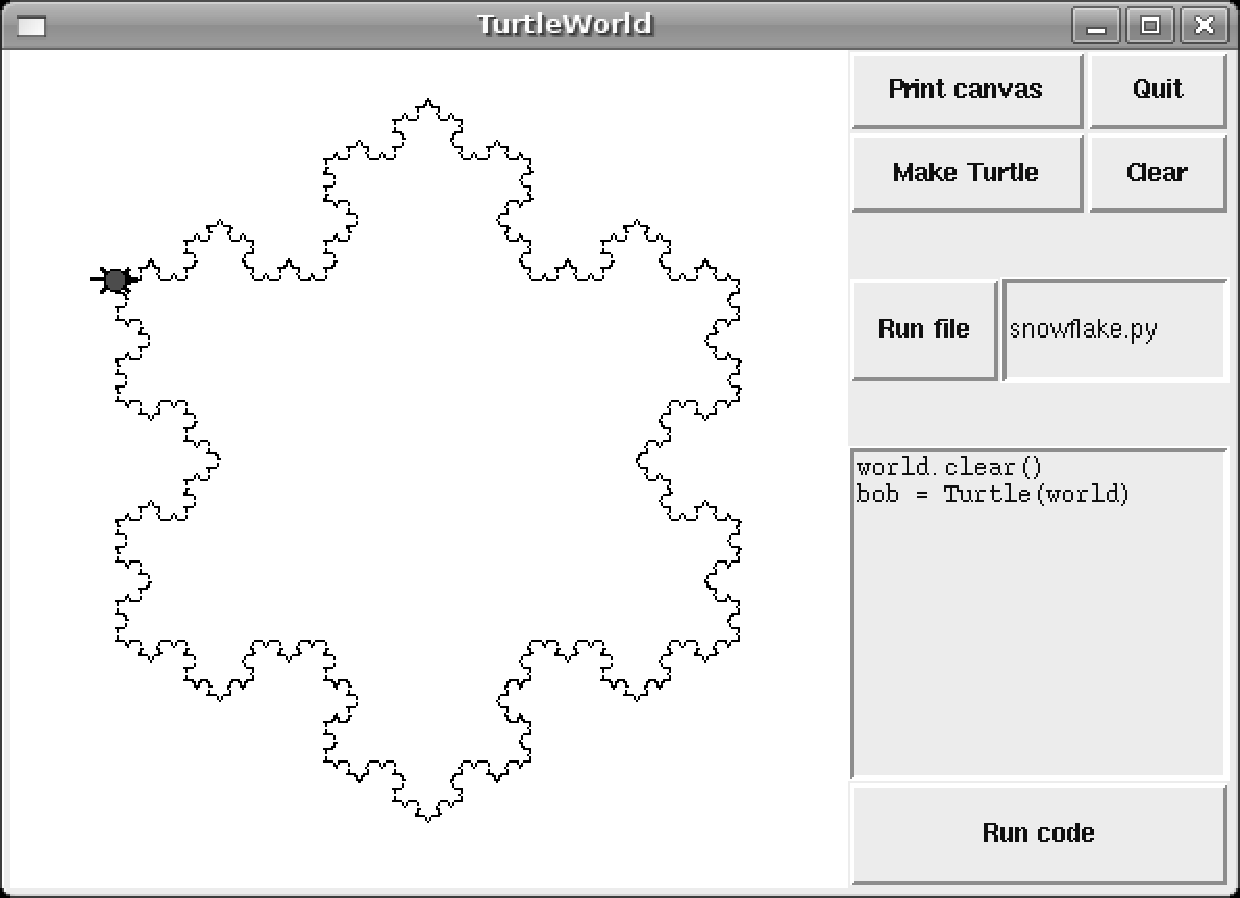
\includegraphics[scale=0.5]{figs/TurtleWorld.pdf}}
\caption{Class diagram.}
\label{fig.turtleworld}
\end{figure}


This section presents the code that creates this GUI, broken into a
series of steps.  You can download the complete example
from \url{http://thinkpython.com/code/SimpleTurtleWorld.py}.

本节展示了创建这个界面的代码,将它拆解为一系列的步骤。你可以在
\url{http://thinkpython.com/code/SimpleTurtleWorld.py}下载完整的代码。

At the top level, this GUI contains two widgets---a Canvas and a
Frame---arranged in a row.  So the first step is to create the row.
\index{SimpleTurtleWorld class}
\index{class!SimpleTurtleWorld}

在最顶层,界面包含了2个组件---一个画布和一个框架---并排放置。所以第一步是指定行
布局。

\begin{verbatim}
class SimpleTurtleWorld(TurtleWorld):
    """This class is identical to TurtleWorld, but the code that
    lays out the GUI is simplified for explanatory purposes."""

    def setup(self):
        self.row()
        ...
\end{verbatim}
%
{\tt setup} is the function that creates and arranges the widgets.
Arranging widgets in a GUI is called {\bf packing}.
\index{packing widgets}
\index{widget, packing}
\index{Frame widget}
\index{widget!Frame}

{\tt setup}方法用来创建和安排组件。对于GUI程序,排放组件称为{\bf packing}

{\tt row} creates a row Frame and makes it the ``current Frame.''
Until this Frame is closed or another Frame is created, all
subsequent widgets are packed in a row.

{\tt row}方法创建了一个横向排列的框架并且把它标记为``当前框架''。直到这个框架关
闭了或者创建了另外一个框架,所有接下来的组件都被打包进了一行。

Here is the code that creates the Canvas and the column Frame
that hold the other widgets:

下面是创建了一个画布和一个容纳其他组件的纵向框架的代码:

\begin{verbatim}
        self.canvas = self.ca(width=400, height=400, bg='white')
        self.col()
\end{verbatim}
%
The first widget in the column is a grid Frame, which contains
four buttons arranged two-by-two:

在纵向框架里面的第一个组建是一个格子框架,又包含了2x2的按钮矩阵:

\begin{verbatim}
        self.gr(cols=2)
        self.bu(text='Print canvas', command=self.canvas.dump)
        self.bu(text='Quit', command=self.quit)
        self.bu(text='Make Turtle', command=self.make_turtle)
        self.bu(text='Clear', command=self.clear)
        self.endgr()
\end{verbatim}
%
{\tt gr} creates the grid; the argument is the number of
columns.  Widgets in the grid are
laid out left-to-right, top-to-bottom.
\index{callback}
\index{bound method}
\index{method, bound}
\index{subject}

{\tt gr}方法创建一个格子;参数是列数。在格子框架里面的组件从左到右,从上到下的
排放。

The first button uses {\tt self.canvas.dump} as a callback; the second
uses {\tt self.quit}.  These are {\bf bound methods}, which means they
are associated with a particular object.  When they are invoked, they
are invoked on the object.

第一个按钮使用{\tt self.canvas.dump}作为回调;第二个使用{\tt self.quit}。这些都
是{\bf 绑定方法},也就是它们和特定的对象绑定到一起的。当它们被调用时,他们是在
对象上被调用的。\footnote{可以简单的理解为对象的方法,self指针会指向对象}

The next widget in the column is a row Frame that contains
a Button and an Entry:

下一个组件是一个包含一个按钮和输入框的横向框架。

\begin{verbatim}
        self.row([0,1], pady=30)
        self.bu(text='Run file', command=self.run_file)
        self.en_file = self.en(text='snowflake.py', width=5)
        self.endrow()
\end{verbatim}
%
The first argument to {\tt row} is a list of weights that
determines how extra space is allocated between widgets.  
The list {\tt [0,1]} means that all extra space is allocated
to the second widget, which is the Entry.  If you run this code
and resize the window, you will see that the Entry grows and
the Button doesn't.

{\tt row}的第一个参数是一个权重列表,决定了组件分配多少的额外空间。
{\tt [0,1]}列表表示所有额外的空间都分给第二个组件,也就是输入狂。如果你运行这段
代码并且重新调整窗口大小,你可以看到输入框变大了而按钮没有变化。

The option {\tt pady} ``pads'' this row in the $y$ direction,
adding 30 pixels of space above and below.

{\tt pady}属性在y轴上下增加了30像素的空白。

{\tt endrow} ends this row of widgets, so subsequent widgets are
packed in the column Frame.  {\tt Gui.py} keeps a stack of Frames:

{\tt endrow}关闭了这个横向框架,所以接下来的组件被打包进入纵向框架。{\tt
Gui.py}维护一个框架的栈:

\begin{itemize}

\item When you use {\tt row}, {\tt col} or {\tt gr} to create a Frame,
it goes on top of the stack and becomes the current Frame.

当你使用{\tt row},{\tt col}或{\tt gr}来创建框架,它进入栈的顶层并且成为当前框
架。

\item When you use {\tt endrow}, {\tt endcol} or {\tt endgr} to close
a Frame, it gets popped off the stack and the previous Frame on the
stack becomes the current Frame.

当你使用{\tt endrow},{\tt endcol}或{\tt endgf}来结束一个框架,它就弹出栈并且上
一个框架成为当前框架。

\end{itemize} 

The method \verb"run_file" reads the contents of the Entry,
uses it as a filename, reads the contents
and passes it to \verb"run_code".  {\tt self.inter} is an
Interpreter object that knows how to take a string and
execute it as Python code.

\verb"run_file" 方法读取输入框的内容,作为文件名,并且读入这个文件,将内容传给
\verb"run_code"。{\tt self.inter}是一个解释器对象,知道如何将这个字符串作为
Python代码来执行。

\begin{verbatim}
    def run_file(self):
        filename = self.en_file.get()
        fp = open(filename)
        source = fp.read()
        self.inter.run_code(source, filename)
\end{verbatim}
%
The last two widgets are a Text widget and a Button:

最后两个组件是一个Text组件和一个按钮:

\begin{verbatim}
        self.te_code = self.te(width=25, height=10)
        self.te_code.insert(END, 'world.clear()\n')
        self.te_code.insert(END, 'bob = Turtle(world)\n')

        self.bu(text='Run code', command=self.run_text)
\end{verbatim}
%
\verb"run_text" is similar to \verb"run_file" except that it takes
the code from the Text widget instead of from a file:

\verb"run_text" 和 \verb"run_file" 比较相似,除了它从一个Text组件而不是文件读入
代码:

\begin{verbatim}
    def run_text(self):
        source = self.te_code.get(1.0, END)
        self.inter.run_code(source, '<user-provided code>')
\end{verbatim}
%
Unfortunately, the details of widget layout are different in
other languages, and in different Python modules.
Tkinter alone provides three different mechanisms for arranging
widgets.  These mechanisms are called {\bf geometry managers}.
The one I demonstrated in this section is the ``grid'' geometry
manager; the others are called ``pack'' and ``place''.
\index{geometry manager}

不幸的是,组件布局的细节在不同的语言中不同,在不同的Python模块中也不同。Tkinter
自己提供了3种不同的机制来安排组件。这些机制被成为几何管理器({\bf geometry
managers})。我在这一节讲述的是``grid''几何管理器;其它的叫``pack''和``place''
。

Fortunately, most of the concepts in this section apply to
other GUI modules and other languages.

幸运的是,本节中的大部分概念都可以用于其它GUI模块和其它语言。

\section{Menus and Callables 菜单和可调用对象}
\index{Menubutton widget}
\index{widget!Menubutton}

A Menubutton is a widget that looks like a button, but when pressed
it pops up a menu.  After the user selects an item, the menu
disappears.

一个菜单按钮是一个看起来像按钮的组件,但是当点击它后会弹出来一个菜单。在用户选
择一个条目后,菜单就消失了。

Here is code that creates a color selection Menubutton
(you can download it from \url{http://thinkpython.com/code/menubutton_demo.py}):

下面是创建一个颜色选择菜单的代码(可以从
\url{http://thinkpython.com/code/menubutton_demo.py}下载)。

\begin{verbatim}
g = Gui()
g.la('Select a color:')
colors = ['red', 'green', 'blue']
mb = g.mb(text=colors[0])
\end{verbatim}
%
{\tt mb} creates the Menubutton.  Initially, the text on the button is
the name of the default color.  The following loop creates one menu
item for each color:

{\tt mb}创建一个菜单按钮。一开始,按钮上的文字是color[0]。接下来的循环用来为每
个颜色创建菜单项。

\begin{verbatim}
for color in colors:
    g.mi(mb, text=color, command=Callable(set_color, color))
\end{verbatim}
%
The first argument of {\tt mi} is the Menubutton these items are
associated with.
\index{callback}
\index{Callable object}
\index{object!Callable}

{\tt mi}的第一个参数是这些菜单项关联的菜单按钮。

The {\tt command} option is a Callable object, which is something new.
So far we have seen functions and bound methods used as callbacks,
which works fine if you don't have to pass any arguments to
the function.  Otherwise you have to construct a Callable object
that contains a function, like \verb"set_color", and its arguments,
like {\tt color}.

{\tt command}按钮是一个可调用对象(函数对象),是一些新东西。我们目前看到的函数和绑定方法用
作回调,你不用传递任何参数给函数就能够正常工作。你也可以创建一个包含函数的可调
用对象,就像\verb"set_color",和它的参数,就像{\tt color}。

The Callable object stores a reference to the function and the
arguments as attributes.  Later, when the user clicks on a menu
item, the callback calls the function and passes the stored
arguments.

可调用对象保存了函数的引用和将要用作属性的参数。之后,当用户点击了一个按钮项,
回调引用的函数,并且把储存的参数传递给它。

Here is what \verb"set_color" might look like:

下面是 \verb"set_color" 长得什么样子的:

\begin{verbatim}
def set_color(color):
    mb.config(text=color)
    print color
\end{verbatim}
%
When the user selects a menu item and \verb"set_color" is called,
it configures the Menubutton to display the newly-selected color.
It also print the color; if you try this example, you can confirm that
\verb"set_color" is called when you select an item (and {\em not}
called when you create the Callable object).

当用户选择了菜单项,\verb"set_color"就被调用了,它使菜单按钮显示新选择的颜色。
它也打印出来颜色值;如果你尝试运行这个例子,你可以确定\verb"set_color"只有当你在
选择了菜单项之后调用(而{\em 不}是在你创建可调用对象时候调用的)。


\section{Binding 绑定}
\index{binding}
\index{callback}

A {\bf binding} is an association between a widget, an event and a
callback: when an event (like a button press) happens on a widget, the
callback is invoked.

一个绑定是在一个组件上和一个事件,回调做关联:当组件上的一个事件(比如点击按钮
)发生了,就会调用回调函数。

Many widgets have default bindings.  For example, when you press
a button, the default binding changes the relief of the button
to make it look depressed.  When you release the button, the
binding restores the appearance of the button and invokes the
callback specified with the {\tt command} option.

许多组件有默认的绑定。例如,当你点击一个按钮,默认的绑定改变按钮的外观让它看起
来像是降低了。当你释放按钮,绑定恢复按钮的外观然后调用使用{\tt command}指定的回
调函数。

You can use the {\tt bind} method to override these default
bindings or to add new ones.  For example, this code creates a
binding for a canvas (you can download the code in this
section from \url{http://thinkpython.com/code/draggable_demo.py}):

你可以使用{\tt bind}方法来覆盖这些默认的绑定或者添加新的。例如,下面的代码为画
布创建了一个绑定(你可以从\url{http://thinkpython.com/code/draggable_demo.py}下
载源代码):

\begin{verbatim}
ca.bind('<ButtonPress-1>', make_circle)
\end{verbatim}
%
The first argument is an event string; this event is triggered
when the user presses the left mouse button.  Other mouse
events include {\tt ButtonMotion}, {\tt ButtonRelease} and
{\tt Double-Button}.
\index{event string}
\index{event handler}

第一个参数是一个事件的名称:当用户点击了鼠标的左键时触发这个时间。其他的鼠标事
件包括{\tt ButtonMotion}, {\tt ButtonRelease}和 {\tt Double-Button}。

The second argument is an event handler.  An event handler
is a function or bound method, like a callback, but an important
difference is that an event handler takes an Event object as a
parameter.  Here is an example:

第二个参数是一个事件句柄。一个事件句柄是一个函数或者绑定方法。比如回调函数,但
是明显不同的是一个事件句柄使用一个Event对象作为参数。下面是一个例子:

\begin{verbatim}
def make_circle(event):
    pos = ca.canvas_coords([event.x, event.y])
    item = ca.circle(pos, 5, fill='red')
\end{verbatim}
%
The Event object contains information about the type of event and
details like the coordinates of the mouse pointer.  In this example
the information we need is
the location of the mouse click.  These
values are in ``pixel coordinates,'' which are defined by the
underlying graphical system.  The method \verb"canvas_coords"
translates them to ``Canvas coordinates,'' which are compatible with
Canvas methods like {\tt circle}.
\index{Event object}
\index{object!Event}

Event对象包含了诸如事件类型和一些类似鼠标指针的坐标等的详细信息。在这个例子中,
我们需要的信息是鼠标点击时的位置。这些值是``像素坐标''\footnote{以左上角为原点
的标准笛卡尔坐标系}。\verb"canvas_coords"方法将这些翻译成和如{\tt circle}等画布
方法兼容的``画布坐标''\footnote{以画布中心为原点的坐标系}。

For Entry widgets, it is common to bind the \verb"<Return>" event,
which is triggered when the user presses the {\sf Return} or
{\sf Enter} key.  For example, the following code creates a Button
and an Entry.

对于输入框组件,常常绑定\verb"<Return>"事件,当用户点击{\sf Return}或者{\sf
Enter}键时触发。例如:下面的代码创建一个按钮和一个输入框。

\begin{verbatim}
bu = g.bu('Make text item:', make_text)
en = g.en()
en.bind('<Return>', make_text)
\end{verbatim}
%
\verb"make_text" is called when the Button is pressed or when
the user hits {\sf Return} while typing in the Entry.  To make
this work, we need a function that can be called as a command
(with no arguments) or as an event handler (with an Event
as an argument):

当点击按钮或者当用户在输入框输入时按{\sf Return}时候触发\verb"make_text" 。为了
使这个工作,我们需要一个可以被作为命令调用(没有参数)或者作为事件句柄(用Event作
为参数)的函数:

\begin{verbatim}
def make_text(event=None):
    text = en.get()
    item = ca.text([0,0], text)
\end{verbatim}
%
\verb"make_text" gets the contents of the Entry and displays
it as a Text item in the Canvas.

\verb"make_text" 获取输入框的内容然后在画布中把它作为一个Text对象显示出来。

It is also possible to create bindings for Canvas items.
The following is a class definition for {\tt Draggable},
which is a child class of {\tt Item} that provides bindings
that implement drag-and-drop capability.
\index{drag-and-drop}

也可以为画布成员创建绑定。下面是一个为{\tt Item}的{\tt Draggable}子类定义的类,
能够提供drag-and-drop能力的绑定。

\begin{verbatim}
class Draggable(Item):

    def __init__(self, item):
        self.canvas = item.canvas
        self.tag = item.tag
        self.bind('<Button-3>', self.select)
        self.bind('<B3-Motion>', self.drag)
        self.bind('<Release-3>', self.drop)
\end{verbatim}
%
The init method takes an Item as a parameter.  It copies
the attributes of the Item and then creates bindings for
three events: a button press, button motion, and button release.

The event handler {\tt select} stores the coordinates
of the current event and the original color of the item, then
changes the color to yellow:

\begin{verbatim}
    def select(self, event):
        self.dragx = event.x
        self.dragy = event.y

        self.fill = self.cget('fill')
        self.config(fill='yellow')
\end{verbatim}
%
{\tt cget} stands for ``get configuration;'' it takes the name of an
option as a string and returns the current value of that option.

{\tt cget} 用来``获取属性'';它用一个属性的名字字符串作为参数然后返回这个属性的当前的值。

{\tt drag} computes how far the object has moved relative to the
starting place, updates the stored coordinates, and then moves the
item.
\index{update!coordinate}

{\tt drag}计算相对起始点,对象被移动了多远,更新储存的坐标,然后移动对象。

\begin{verbatim}
    def drag(self, event):
        dx = event.x - self.dragx
        dy = event.y - self.dragy

        self.dragx = event.x
        self.dragy = event.y

        self.move(dx, dy)
\end{verbatim}
%
This computation is done in pixel coordinates; there is no need to
convert to Canvas coordinates.
\index{Canvas coordinate}
\index{coordinate!Canvas}
\index{pixel coordinate}
\index{coordinate!pixel}

这个是用像素坐标计算的;这里没有必要转换成画布坐标。

Finally, {\tt drop} restores the original color of the item:

最后,{\tt drop}恢复对象的原来的颜色:

\begin{verbatim}
    def drop(self, event):
        self.config(fill=self.fill)
\end{verbatim}
%
You can use the {\tt Draggable} class to add drag-and-drop
capability to an existing item.  For example, here is a modified
version of \verb"make_circle" that uses {\tt circle} to create
an Item and {\tt Draggable} to make it draggable:

你可以使用{\tt Draggable}类来为一个已经存在的对象增加drag-and-drop功能。例如,
下面是一个修改版的\verb"make_circle",使用{\tt circle}来创建一个对象然后使用
{\tt Draggable}来使它可拖动:

\begin{verbatim}
def make_circle(event):
    pos = ca.canvas_coords([event.x, event.y])
    item = ca.circle(pos, 5, fill='red')
    item = Draggable(item)
\end{verbatim}
%
This example demonstrates one of the benefits of inheritance: you can
modify the capabilities of a parent class without modifying its
definition.  This is particularly useful if you want to change
behavior defined in a module you did not write.

这个例子解释了继承的一个好处:你可以增减一个父类的功能而不用修改其定义。当你想
改变一个不是你写的模块里面的类的行为时就非常有用。


\section{Debugging 调试}
\index{debugging}

One of the challenges of GUI programming is keeping track of
which things happen while the GUI is being built and which
things happen later in response to user events.
\index{callback}

一个GUI编程的挑战是跟踪GUI创建时发生了什么事以及什么是在延迟到用户事件时发生的
事情。

For example, when you are setting up a callback, it is a common error
to call the function rather than passing a reference to it:

例如,当你设置了一个回调,常见的错误是直接调用了这个函数而不是传递它的一个引用:

\begin{verbatim}
def the_callback():
    print 'Called.'

g.bu(text='This is wrong!', command=the_callback())
\end{verbatim}
%
If you run this code, you will see that it calls \verb"the_callback"
immediately, and {\em then} creates the button.  When you press the
button, it does nothing because the return value from 
\verb"the_callback" is {\tt None}.
Usually you do not want to invoke a callback while you are
setting up the GUI; it should only be invoked later in response to
a user event.
\index{flow of execution}
\index{event-driven programming}

如果你运行这个代码,你会立刻看到它调用了\verb"the_callback",然后创建按钮。当你
点击按钮时,什么都没有发生。因为\verb"the_callback"的返回值是{\tt None}。
通常你不想在你设置GUI的时候调用回调函数;它应该在之后的响应用户事件时调用。

Another challenge of GUI programming is that you don't have control
of the flow of execution.  Which parts of the program execute
and their order are determined by user actions.
That means that you have to design your program to work correctly
for any possible sequence of events.

GUI编程的另外一个挑战是你并不能控制执行流程。哪部分的程序执行以及执行的顺序是由
用户动作决定的。也就是说你必须为任何可能的时间序列设计正确运行的程序。

For example, the GUI in Exercise~\ref{circle2} has two widgets:
one creates a Circle item and the other changes the color of the
Circle.  If the user creates the circle and then changes its color,
there's no problem.  But what if the user changes the color of
a circle that doesn't exist yet?  Or creates more than one circle?

例如,在~\ref{circle2}练习中的GUI有两个组件:一个创建圆另外一个更改圆的颜色。如
果用户先创建一个圆再改变颜色就没有问题。但是如果用户先改变颜色后创建圆?或者创
建了多个圆呢?

As the number of widgets grows, it is increasingly difficult to
imagine all possible sequences of events.  One way to manage this 
complexity is to encapsulate the state of the system in an object
and then consider:

当组件的数量增加时,想象所有可能的事件序列就变得非常困难。一种管理这种麻烦事的
方法是把它们封装进状态系统,然后再考虑:

\begin{itemize}

\item What are the possible states?  In the Circle example, we
might consider two states: before and after the user creates the
first circle.

可能的状态有哪些?在圆例子中,我们可以考虑两个状态:用户创建了第一个圆之前和之
后两个状态。

\item In each state, what events can occur?  In the example,
the user can press either of the buttons, or quit.

在每个状态,会发生什么事件?在本例中,用户可以点击按钮或者退出。

\item For each state-event pair, what is the desired outcome?
Since there are two states and two buttons, there are four
state-event pairs to consider.

在每一个状态-事件对,设计好的结果是什么?因为这里有2个状态和2个按钮。所以需要考
虑4个状态-事件对。

\item What can cause a transition from one state to another?
In this case, there is a transition when the user creates
the first circle.

什么能够造成一种状态迁移到另外一种状态?在本例中,当用户创建了第一个圆之后有一
个迁移。

\end{itemize}

You might also find it useful to define, and check, invariants that
should hold regardless of the sequence of events.
\index{invariant}

% ??? %

This approach to GUI programming can help you write correct
code without taking the time to test every possible sequence
of user events!

这些GUI编程的途径能够帮助你写正确的代码而不用花时间测试每个可能的用户事件顺序!


\section{Glossary 术语表}

\begin{description}

\item[GUI:] A graphical user interface.
\index{GUI}

\item[widget(组件):] One of the elements that makes up a GUI, including
buttons, menus, text entry fields, etc. 
\index{widget}

\item[option(属性):] A value that controls the appearance or function of
a widget.
\index{option}

\item[keyword argument(关键字参数):] An argument that indicates the parameter
name as part of the function call.
\index{keyword argument}

\item[callback(回调):] A function associated with a widget that is
called when the user performs an action.
\index{callback}

\item[bound method(对象方法):] A method associated with a particular instance.
\index{bound method}

\item[event-driven programming(事件驱动编程):] A style of programming in which
the flow of execution is determined by user actions.
\index{event-driven programming}

\item[event(事件):] A user action, like a mouse click or key press, that
causes a GUI to respond.
\index{event}

\item[event loop(事件循环):] An infinite loop that waits for user actions
and responds.
\index{event loop}

\item[item:] A graphical element on a Canvas widget.
\index{item!Canvas}

\item[bounding box:] A rectangle that encloses a set of items,
usually specified by two opposing corners.
\index{bounding box}

\item[pack(打包):] To arrange and display the elements of a GUI.
\index{packing widgets}

\item[geometry manager(几何管理器):] A system for packing widgets.
\index{geometry manager}

\item[binding(绑定):] An association between a widget, an event, and
an event handler.  The event handler is called when the event
occurs in the widget.
\index{binding}

\end{description}


\section{Exercises 练习}

\begin{exercise}
\index{image viewer}

For this exercise, you will write an image viewer.  Here is
a simple example:

在这个练习中,你需要写一个图像浏览器。下面是一个简单的例子:

\begin{verbatim}
g = Gui()
canvas = g.ca(width=300)
photo = PhotoImage(file='danger.gif')
canvas.image([0,0], image=photo)
g.mainloop()
\end{verbatim}
%
{\tt PhotoImage} reads a file and returns a {\tt PhotoImage} object
that Tkinter can display.  {\tt Canvas.image} puts the image on the
canvas, centered on the given coordinates.  You can also put images on
labels, buttons, and some other widgets:

{\tt PhotoImage} 读取一个文件然后返回一个Tkinter可以显示的{\tt PhotoImage}对象
。{\tt Canvas.Image}把这些图像放到canvas中,根据给定的坐标居中。你也可以其在图
像上放一个标签,按钮,和其它的组件。

\begin{verbatim}
g.la(image=photo)
g.bu(image=photo)
\end{verbatim}
%
PhotoImage can only handle a few image formats, like GIF and PPM, 
but we can use the Python Imaging Library (PIL) to read other
files.
\index{Python Imaging Library (PIL)}
\index{PIL (Python Imaging Library)}
\index{Image module}
\index{module!Image}

PhotoImage可以只处理几个图像格式,比如GIF和PPM,我们也可以使用Python Imageing
Library (PIL)来读取其它格式。

The name of the PIL module is {\tt Image}, but Tkinter defines an
object with the same name.  To avoid the conflict, you can use {\tt
  import...as} like this:

PIL模块的名称是{\tt Image}。但是Tkinter定义了一个相同名称的对象。为了避免冲突,
你可以使用{\tt import...as}来解决。

\begin{verbatim}
import Image as PIL
import ImageTk
\end{verbatim}
%
The first line imports {\tt Image} and
gives it the local name {\tt PIL}.  The second
line imports {\tt ImageTk}, which can translate a PIL
image into a Tkinter PhotoImage.  Here's an example:

第一行导入{\tt Image}然后给予一个本地名称{\tt PIL}。第二行导入{\tt ImageTk},可
以将PIL图像转换成一个Tkinter PhotoImage。下面是一个例子:

\begin{verbatim}
image = PIL.open('allen.png')
photo2 = ImageTk.PhotoImage(image)
g.la(image=photo2)
\end{verbatim}
%

\begin{enumerate}

\item Download \verb"image_demo.py", \verb"danger.gif" and \verb"allen.png"
from \url{http://thinkpython.com/code}.  Run \verb"image_demo.py".  You
might have to install {\tt PIL} and {\tt ImageTk}.  
They are probably in your software repository,  but if not
you can get them from \url{pythonware.com/products/pil/}.


从 \url{http://thinkpython.com/code}下载\verb"image_demo.py", \verb"danger.gif"
和 \verb"allen.png" .  运行 \verb"image_demo.py".  你可能需要先去安装 {\tt PIL}
和 {\tt ImageTk}。它们可能在你的软件源中,  如果不是的话,你可以从
\url{pythonware.com/products/pil/}下载。

\item In \verb"image_demo.py" change the name of the second
PhotoImage from {\tt photo2} to {\tt photo} and run the program
again.  You should see the second PhotoImage but not the first.

在\verb"image_demo.py"将第二个PhotoImage的名字从 {\tt photo2} 改为{\tt photo}
然后再次运行程序。你可以看到第二个PhotoImage而不是第一个。

The problem is that when you reassign {\tt photo} it overwrites
the reference to the first PhotoImage, which then disappears.  The
same thing happens if you assign a PhotoImage to a local
variable; it disappears when the function ends.

问题是你重新赋值的{\tt photo}覆盖了第一个PhotoImage的引用,所以消失了。同样地如
果你把一个PhotoImage赋值为一个局部变量;在函数结束时它也会消失。

To avoid this problem, you have to store a reference to each
PhotoImage you want to keep.  You can use a global variable, or
store PhotoImages in a data structure or as an attribute of
an object.

为了避免这个问题,你可以储存每一个你想保留的PhotoImage的引用。你可以使用一个全
局变量,或者把PhotoImage储存在一个作为对象的属性的数据结构中。

This behavior can be frustrating, which is why I am warning
you (and why the example image says ``Danger!'').
\index{bug!worst ever}
\index{worst bug!ever}

这样做可能会让人迷惑,所以我要警告你(也是为什么这个例子用的图片是``Danger!'')。

\item Starting with this example, write a program that takes
the name of a directory and loops through all the files, displaying
any files that PIL recognizes as images.  You can use a {\tt try}
statement to catch the files PIL doesn't recognize.

由这个例子开始,写一个程序,用一个文件夹名字作为输入然后遍历所有文件,显示那些
PIL可以识别的任何图像文件。你可以使用一个{\tt try}语句来捕获PIL不能识别的文件。

When the user clicks on the image, the program should display the next one.

当用户点击图片,程序应该显示下一个。

\item PIL provides a variety of methods for manipulating images.
You can read about them at \url{http://pythonware.com/library/pil/handbook}.
As a challenge, choose a few of these methods and provide a
GUI for applying them to images.

PIL提供了众多的方法来处理图像。你可以在
\url{http://pythonware.com/library/pil/handbook}阅读。作为一个挑战,从这些方法
中选择几个然后提供一个GUI来应用它们到图像上。

\end{enumerate}

Solution: \url{http://thinkpython.com/code/ImageBrowser.py}.

\end{exercise}


\begin{exercise}
\index{vector graphics}
\index{SVG}

A vector graphics editor is a program that allows users to draw and
edit shapes on the screen and generate output files in vector graphics
formats like Postscript and SVG.

一个矢量图编辑器是一个可以允许用户在屏幕上绘制和编辑图形并且用如Postscript和SVG
的矢量图格式生成输出文件的软件。

Write a simple vector graphics editor using Tkinter.  At a
minimum, it should allow users to draw lines, circles and
rectangles, and it should use {\tt Canvas.dump} to
generate a Postscript description of the contents of the
Canvas.

用Tkinter写一个简单的矢量图编辑器。至少,它应该允许用户绘制直线,圆和矩形,它应
该使用{\tt Canvas.dump}来把画布的内容生成为Postscript。

As a challenge, you could allow users to select and resize
items on the Canvas.

作为一个挑战,你可以允许用户选择和缩放画布上的元素。

% TODO: write a solution!

\end{exercise}


\begin{exercise}

Use Tkinter to write a basic web browser.  It
should have a Text widget where the user can enter a URL
and a Canvas to display the contents of the page.
\index{urllib module}
\index{module!urllib}
\index{URL}
\index{HTMLParser module}
\index{module!HTMLParser}

使用Tkinter写一个简单的网页浏览器。它应该有一个Text组件来让用户输入一个URL和一
个画布来显示网页的内容。

You can use the {\tt urllib} module to download files
(see Exercise~\ref{urllib}) and
the {\tt HTMLParser} module to parse the HTML
tags (see \url{docs.python.org/lib/module-HTMLParser.html}).
\index{plain text}
\index{text!plain}
\index{hyperlink}

你可以使用{\tt urllib}模块来下载文件(参见 ~\ref{urllib}练习)和{\tt
HTMLParser}模块来处理HTML标签(参见
\url{docs.python.org/lib/module-HTMLParser.html})。

At a minimum your browser should handle plain text and hyperlinks.  As
a challenge you could handle background colors, text
formatting tags and images.

至少,你的浏览器应该处理纯文本和超链接。作为一个挑战你可以处理背景颜色,文字格
式化标签和图像。

% TODO: write a solution!

\end{exercise}



\appendix

\chapter{Debugging 调试}

% translate by xiehuc (xiehuc@gmail.com)

\index{debugging}
Different kinds of errors can occur
in a program, and it is useful to distinguish among them
in order to track them down more quickly:

在一个程序中可能会发生各种各样的错误,为了能够快速的追踪到这些错误,能够从代码
中辨识出错误是非常有用的:

\begin{itemize}

\item Syntax errors are produced by Python when it is translating the
  source code into byte code.  They usually indicate that there is
  something wrong with the syntax of the program.  Example: Omitting
  the colon at the end of a {\tt def} statement yields the somewhat
  redundant message {\tt SyntaxError: invalid syntax}.

  语法错误是Python将源代码翻译成字节代码的时候产生的。他们通常预示着程序的语法
  有一些错误。例如:省略了{\tt def}语句后面的冒号会产生一些冗余的信息 {\tt
  SyntaxError: invalid syntax}.

\item Runtime errors are produced by the interpreter if something goes
  wrong while the program is running.  Most runtime error messages
  include information about where the error occurred and what
  functions were executing.  Example: An infinite recursion eventually
  causes the runtime error ``maximum recursion depth exceeded.''

  运行时错误是当程序运行时发生了一些错误,解释器产生的错误。大多数运行时错误会
  包含诸如在哪里产生的错误和正在执行哪个函数等信息。例如:一个无限递归最终会造
  成``超过递归最大深度''的错误。

\item Semantic errors are problems with a program that runs without
  producing error messages but doesn't do the right thing.  Example:
  An expression may not be evaluated in the order you expect, yielding
  an incorrect result.

  语义错误是指一个程序并没有抛出错误信息,但是没有做正确的事情\footnote{译者注
  :一般是由于代码编写错误}。例如:一个表达式可能因为没有按照你预期的执行顺序而
  被略过了没有执行,因此产生了错误的结果。

\end{itemize}
\index{syntax error}
\index{runtime error}
\index{semantic error}
\index{error!compile-time}
\index{error!syntax}
\index{error!runtime}
\index{error!semantic}
\index{exception}

The first step in debugging is to figure out which kind of
error you are dealing with.  Although the following sections are
organized by error type, some techniques are
applicable in more than one situation.

调试的第一步是指出你正在处理那种错误。虽然下面的小节按照错误类型来组织的,一些
方法能应用在更多的情况下。

\section{Syntax errors 语法错误}
\index{error message}

Syntax errors are usually easy to fix once you figure out what they
are.  Unfortunately, the error messages are often not helpful.
The most common messages are {\tt SyntaxError: invalid syntax} and
{\tt SyntaxError: invalid token}, neither of which is very informative.

语法错误通常一旦找出它们,就容易修正。不幸的是,这些错误消息可能没什么帮助。最
常见的错误消息是{\tt SyntaxError: invalid syntax}和{\tt SyntaxError: invalid
token},都不是很有用。

On the other hand, the message does tell you where in the program the
problem occurred.  Actually, it tells you where Python
noticed a problem, which is not necessarily where the error
is.  Sometimes the error is prior to the location of the error
message, often on the preceding line.
\index{incremental development}
\index{development plan!incremental}

另一方面,这些错误消息并不告诉你程序的哪里出现的错误。实际上,它告诉你Python是
在哪里发现的问题,和错误具体在哪里无关。有时,错误在消息提示的代码的前面,通常
则是在后面。

If you are building the program incrementally, you should have
a good idea about where the error is.  It will be in the last
line you added.

如果你是一点一点地增量式地写的代码,你应该能够知道错误在哪里。它会在你最后写的
几行代码中。

If you are copying code from a book, start by comparing
your code to the book's code very carefully.  Check every character.
At the same time, remember that the book might be wrong, so
if you see something that looks like a syntax error, it might be.

如果你是从书上复制的代码,那请仔细地从头和书对照代码。一个一个字母地比照。不过
,另外,也可能是书上就错了,所以如果你发现哪里就像是语法错误,那可能就是了。

Here are some ways to avoid the most common syntax errors:

下面是一些方法用于避免大部分常见的语法错误:
\index{syntax}

\begin{enumerate}

\item Make sure you are not using a Python keyword for a variable name.
\index{keyword}

确保你没有使用Python的关键字作为变量名称。

\item Check that you have a colon at the end of the header of every
compound statement, including {\tt for}, {\tt while},
{\tt if}, and {\tt def} statements.
\index{header}
\index{colon}

检查你每个复合语句的首行的末尾都有冒号,包括{\tt for}, {\tt while},
{\tt if}, 和 {\tt def} 语句。

\item Make sure that any strings in the code have matching
quotation marks.
\index{quotation mark}

确保你的字符串都有匹配地引号。

\item If you have multiline strings with triple quotes (single or double), make
sure you have terminated the string properly.  An unterminated string
may cause an {\tt invalid token} error at the end of your program,
or it may treat the following part of the program as a string until it
comes to the next string.  In the second case, it might not produce an error
message at all!
\index{multiline string}
\index{string!multiline}

如果你有三引号地多行字符串,确保你合适的结束了字符串。一个没有结束的字符串会在
程序的末尾产生{\tt invalid token}错误,或者它会吧剩下的程序部分的代码看作字符串
的一部分,直到遇到下一个三引号字符串。第二种情况可能直接不会产生错误!
\footnote{有语法着色功能的编辑器则能够方便的看出}

\item An unclosed opening operator---\verb+(+, \verb+{+, or
  \verb+[+---makes Python continue with the next line as part of the
  current statement.  Generally, an error occurs almost immediately in
  the next line.

  一个没有关闭的括号(\verb+(+, \verb+{+, 以及 \verb+[+)使得Python把下一行继续
          看作当前语句的一部分。通常下一行会马上提示错误消息。

\item Check for the classic {\tt =} instead of {\tt ==} inside
a conditional.
\index{conditional}

检查条件语句里面的{\tt ==}是不是写成了{\tt =}。

\item Check the indentation to make sure it lines up the way it
is supposed to.  Python can handle space and tabs, but if you mix
them it can cause problems.  The best way to avoid this problem
is to use a text editor that knows about Python and generates
consistent indentation.
\index{indentation}
\index{whitespace}

确保每行地缩进是符合语法地。Python能够处理空格和Tab,但是如果你混用它们可能出错
。最好的方法是使用一个了解Python语法的纯文本编辑器\footnote{如llinux下面的vim,
跨平台的sublime text等等}来产生一致的缩进。

\end{enumerate}

If nothing works, move on to the next section...

如果还是不行,请看下一节。。。


\subsection{I keep making changes and it makes no difference. \\ 我不断的改代码似乎一点用都没有。}

If the interpreter says there is an error and you don't see it, that
might be because you and the interpreter are not looking at the same
code.  Check your programming environment to make sure that the
program you are editing is the one Python is trying to run.

如果翻译器说这里有一个错误但是你怎么也看不出来,可能是因为你和翻译器没有看同一
份代码。检查你的编码环境确保你正在编辑的就是Python尝试运行的。

If you are not sure, try putting an obvious and deliberate syntax
error at the beginning of the program.  Now run it again.  If the
interpreter doesn't find the new error, you are not running the
new code.

如果你不确定,尝试在代码的开始制造一些明显的故意的语法错误。再运行一次。如果翻
译器不能找出新的错误,说明你没有运行正确的文件。

There are a few likely culprits:

\begin{itemize}

\item You edited the file and forgot to save the changes before
running it again.  Some programming environments do this
for you, but some don't.

你编辑了文件忘记了在运行之前保存一下。有一些编程环境会在运行前自动保存,有些则
不会。

\item You changed the name of the file, but you are still running
the old name.

你更改了文件的名字,但是你任然运行旧名字的文件。

\item Something in your development environment is configured
incorrectly.

你开发环境的一些配置不正确。

\item If you are writing a module and using {\tt import},
make sure you don't give your module the same name as one
of the standard Python modules.
\index{module!reload}
\index{reload function}
\index{function!reload}

如果你在用{\tt import}写一个模块,确保你没有使用标准的Python模块名作为你的模块的
名字。

\item If you are using {\tt import} to read a module, remember
that you have to restart the interpreter or use {\tt reload}
to read a modified file.  If you import the module again, it
doesn't do anything.

如果你使用{\tt import}来载入一个模块,记住你必须重启翻译器才能重新载入一个修改
了的内存模块。如果你导入一个模块两次,第二次是无效的。\footnote{译者注:因为载
入的模块在内存中,如果不退出翻译器,是不会释放在内存中的模块的。通常是在交互式
的换进中才会有该问题}

\end{itemize}

If you get stuck and you can't figure out what is going on, one
approach is to start again with a new program like ``Hello, World!,''
and make sure you can get a known program to run.  Then gradually add
the pieces of the original program to the new one.

如果你依然卡住了,不知道怎么办,一种途径是重新开始一个新的``Hello, World!''程序
,确保你能运行一个已知的程序。然后逐渐地把原来程序的代码粘贴到新的里面。

\section{Runtime errors 运行时错误}

Once your program is syntactically correct,
Python can compile it and at least start running it.  What could
possibly go wrong?

一旦你的程序语法正确,Python就至少能够编译它,并且运行它。然后可能会出现哪些错
误?

\subsection{My program does absolutely nothing.\\我的程序什么也没有做}

This problem is most common when your file consists of functions and
classes but does not actually invoke anything to start execution.
This may be intentional if you only plan to import this module to
supply classes and functions.

这个问题最可能是当你的文件由函数和类组成,但是并没有调用任何东西来执行。可能是
因为你只是打算导入这个模块来提供类和函数。

If it is not intentional, make sure that you
are invoking a function to start execution, or execute one from
the interactive prompt.  Also see the ``Flow of Execution'' section
below.

如果你不是想这样的,确保你调用了一个函数来开始执行。或从交互式终端执行一个函数
。参见下面 ``Flow of Execution'' 一节

\subsection{My program hangs. \\ 我的程序挂了}
\index{infinite loop}
\index{infinite recursion}
\index{hanging}

If a program stops and seems to be doing nothing, it is ``hanging.''
Often that means that it is caught in an infinite loop or infinite
recursion.

如果一个程序停止了,看起来什么都没有做,这就是 ``挂''了。通常意味着它陷入了一个
无限循环或者是无限递归。

\begin{itemize}

\item If there is a particular loop that you suspect is the
problem, add a {\tt print} statement immediately before the loop that says
``entering the loop'' and another immediately after that says
``exiting the loop.''

如果正好有一个你怀疑可能出问题的循环,在进入循环之前加入一个 {\tt print} 语句,
打印 ``entering the loop'',然后在循环结束之后同样的打印``exit the loop''。

Run the program.  If you get the first message and not the second,
you've got an infinite loop.  Go to the ``Infinite Loop'' section
below.

运行程序。 如果你只得到了第一条信息但是没有第二条,那就是进入无限循环了。转到``
无限循环''一节

\item Most of the time, an infinite recursion will cause the program
to run for a while and then produce a ``RuntimeError: Maximum
recursion depth exceeded'' error.  If that happens, go to the
``Infinite Recursion'' section below.

大多数情况,一个无限递归会造成程序运行一会儿之后输出``RuntimeError: Maximum
recursion depth exceeded''错误。如果发生了,转到``无限递归''一节。

If you are not getting this error but you suspect there is a problem
with a recursive method or function, you can still use the techniques
in the ``Infinite Recursion'' section.

如果你没有得到这个错误,但是你坚持怀疑可能是一个递归调用出问题了,你也可以使用
``无限递归''一节的技巧。

\item If neither of those steps works, start testing other
loops and other recursive functions and methods.

如果两种都不行,测试一下其它循环或者递归调用。

\item If that doesn't work, then it is possible that
you don't understand the flow of execution in your program.
Go to the ``Flow of Execution'' section below.

如果还是不行,可能是你没有正确的理解你的程序的执行流程。转到``Flow of Execution''一节。

\end{itemize}


\subsubsection{Infinite Loop 无限循环}
\index{infinite loop}
\index{loop!infinite}
\index{condition}
\index{loop!condition}

If you think you have an infinite loop and you think you know
what loop is causing the problem, add a {\tt print} statement at
the end of the loop that prints the values of the variables in
the condition and the value of the condition.

For example:

如果你认为你有一个无限循环并且你知道是这个循环造成的问题,在每个循环的末尾加入
{\tt print}语句,打印出循环条件中变量的值和运算的结果。

例如:

\begin{verbatim}
while x > 0 and y < 0 :
    # do something to x
    # do something to y

    print "x: ", x
    print "y: ", y
    print "condition: ", (x > 0 and y < 0)
\end{verbatim}
%
Now when you run the program, you will see three lines of output
for each time through the loop.  The last time through the
loop, the condition should be {\tt false}.  If the loop keeps
going, you will be able to see the values of {\tt x} and {\tt y},
and you might figure out why they are not being updated correctly.

现在,当你运行程序,你可以看到每次循环都有3行输出。最后一次输出时,循环条件应该
是{\tt false}。如果循环继续走下去,你能够看到{\tt x} 和{\tt y}的至,因此你可以
了解到为什么它们没有被正确的更新。

\subsubsection{Infinite Recursion 无限递归}
\index{infinite recursion}
\index{recursion!infinite}

Most of the time, an infinite recursion will cause the program to run
for a while and then produce a {\tt Maximum recursion depth exceeded}
error.

大多数情况,一个无限递归会造成程序运行一会儿之后输出``RuntimeError: Maximum
recursion depth exceeded''错误。如果发生了,转到``无限递归''一节。

If you suspect that a function or method is causing an infinite
recursion, start by checking to make sure that there is a base case.
In other words, there should be some condition that will cause the
function or method to return without making a recursive invocation.
If not, then you need to rethink the algorithm and identify a base
case.

如果你怀疑一个函数或者方法造成了无限递归,确保函数体有一个初始条件。也就是有一
些条件能够直接返回值而不会再递归调用下去。如果没有,你需要重新思考算法找到一个
初始条件。

If there is a base case but the program doesn't seem to be reaching
it, add a {\tt print} statement at the beginning of the function or method
that prints the parameters.  Now when you run the program, you will see
a few lines of output every time the function or method is invoked,
and you will see the parameters.  If the parameters are not moving
toward the base case, you will get some ideas about why not.

如果有了初始条件了但是程序还是没有到达它,在函数或方法的开始加入一个{\tt print}
语句来打印参数。现在当你运行程序,每次递归调用你都能看到几行输出,你可以看到参
数。如果参数没有趋于初始条件,你需要想想为什么。

\subsubsection{Flow of Execution 执行流}
\index{flow of execution}

If you are not sure how the flow of execution is moving through
your program, add {\tt print} statements to the beginning of each
function with a message like ``entering function {\tt foo},'' where
{\tt foo} is the name of the function.

如果你不确定程序执行的过程,在每个函数的开始打印``entering function {\tt
foo}'',{\tt foo}是你的函数名。

Now when you run the program, it will print a trace of each
function as it is invoked.

现在当你运行程序,你可以打印出每个函数调用的轨迹。

\subsection{When I run the program I get an exception.\\当我运行程序时产生了异常}
\index{exception}
\index{runtime error}

If something goes wrong during runtime, Python
prints a message that includes the name of the
exception, the line of the program where the problem occurred,
and a traceback.
\index{traceback}

如果在运行时出现了问题,Python会打印出一些信息,包括异常的名称,产生一场的行号
,和一个调用栈。

The traceback identifies the function that is currently running,
and then the function that invoked it, and then the function that
invoked {\em that}, and so on.  In other words, it traces the
sequence of function invocations that got you to where you are.  It
also includes the line number in your file where each of these
calls occurs.

调用栈(backtrace,traceback,callstack)能够表明正在运行的函数,以及调用它的上层
函数,上上层函数等等。总之,它表明了函数调用的顺序以及运行到哪里了。它也包含源
代码中产生调用的地方的行号

The first step is to examine the place in the program where
the error occurred and see if you can figure out what happened.
These are some of the most common runtime errors:

第一步是检查发生错误的位置,看你能不能找出怎么就错了。下面是一些常见错误

\begin{description}

\item[NameError:]  You are trying to use a variable that doesn't
exist in the current environment.
Remember that local variables are local.  You
cannot refer to them from outside the function where they are defined.
\index{NameError}
\index{TypeError}
\index{exception!NameError}
\index{exception!TypeError}

命名错误:你正在使用当前上下文中不存在的变量名。记住局部变量是有作用域的。你不
能在函数的外面引用它们。

\item[TypeError:] There are several possible causes:

    类型错误:有几种可能的原因:

\begin{itemize}

\item  You are trying to use a value improperly.  Example: indexing
a string, list, or tuple with something other than an integer.
\index{index}

你正在不正确的使用一个值。例如:使用除整数以外的某些东西作为字符串,列表或元组
的索引下标。

\item There is a mismatch between the items in a format string and
the items passed for conversion.  This can happen if either the number
of items does not match or an invalid conversion is called for.
\index{format operator}
\index{operator!format}


\item You are passing the wrong number of arguments to a function or method.
For methods, look at the method definition and
check that the first parameter is {\tt self}.  Then look at the
method invocation; make sure you are invoking the method on an
object with the right type and providing the other arguments
correctly.

你传递错误数量的参数给函数或方法。对于方法,看看方法定义是不是以{\tt self}作为
地一个参数。然后看看方法调用;确保你在一个正确的类型的对象上调用方法并且正确得
提供了其它参数。

\end{itemize}

\item[KeyError:]  You are trying to access an element of a dictionary
using a key that the dictionary does not contain.
\index{KeyError}
\index{exception!KeyError}
\index{dictionary}

键错误:你尝试用字典没有的键来访问字典的元素。

\item[AttributeError:] You are trying to access an attribute or method
that does not exist.  Check the spelling!  You can use
{\tt dir} to list the attributes that do exist.

属性错误:你尝试访问一个不存在的属性或方法。检查一下拼写!你可以使用{\tt dir}来
列出存在的属性。

If an AttributeError indicates that an object has {\tt NoneType},
that means that it is {\tt None}.  One common cause is forgetting
to return a value from a function; if you get to the end of
a function without hitting a {\tt return} statement, it returns
{\tt None}.  Another common cause is using the result from
a list method, like {\tt sort}, that returns {\tt None}.
\index{AttributeError}
\index{exception!AttributeError}

如果一个属性错误表明一个对象是{\tt NoneType},那意味着它就是{\tt None}。一个常
见的原因是忘记从函数返回一个值;如果你在函数的末尾没有写{\tt return}语句,它就
会返回{\tt None}。另外一个原因是使用一个list的方法调用的结果,比如{\tt sort}就
会返回{\tt None}。

\item[IndexError:] The index you are using
to access a list, string, or tuple is greater than
its length minus one.  Immediately before the site of the error,
add a {\tt print} statement to display
the value of the index and the length of the array.
Is the array the right size?  Is the index the right value?
\index{IndexError}
\index{exception!IndexError}

索引错误:你访问一个列表,字符串或元组的索引超过了它的长度-1。在这类错误的前面
,用一个{\tt print}语句来打印索引的值和数组的长度。数组是有着正确的长度吗?索引
是正确的吗?

\end{description}
\index{debugger (pdb)}
\index{Python debugger (pdb)}
\index{pdb (Python debugger)}

The Python debugger ({\tt pdb}) is useful for tracking down
Exceptions because it allows you to examine the state of the
program immediately before the error.  You can read
about {\tt pdb} at \url{docs.python.org/lib/module-pdb.html}.

Python debugger ({\tt pdf})是用来追踪异常的非常有用的工具,因为它让你可以检查程
序在出现错误时的状态。而不是直接的退出。你可以阅读
\url{docs.python.org/lib/module-pdb.html}关于{\tt pdb}一节。

\subsection{I added so many {\tt print} statements I get inundated with
output.\\我加入了太多的{\tt print}语句以至于输出刷屏}
\index{print statement}
\index{statement!print}

One of the problems with using {\tt print} statements for debugging
is that you can end up buried in output.  There are two ways
to proceed: simplify the output or simplify the program.

使用{\tt print}语句来调试的一个问题是你可能会被泛滥的输出所埋没。有两种途径来处
理:简化输出或者是简化程序。

To simplify the output, you can remove or comment out {\tt print}
statements that aren't helping, or combine them, or format
the output so it is easier to understand.

为了简化输出,你可以移除或注释掉不再需要的{\tt print}语句,或者合并它们,或者格
式化输出便于理解。\footnote{也可以采用c的宏定义的思想,使用一个ENABLE\_DEBUG的
全局变量,然后使用{\tt if(ENABLE\_DEBUG) print(...)}这种,通过将ENABLE\_DEBUG赋
值为false来关闭所有输出。}\footnote{再层次化的输出就被称为Log了。也是一种必要的
调试方法}

To simplify the program, there are several things you can do.  First,
scale down the problem the program is working on.  For example, if you
are searching a list, search a {\em small} list.  If the program takes
input from the user, give it the simplest input that causes the
problem.
\index{dead code}

为了简化程序,有几件事情可以做的。首先,缩减当前求解问题的规模。例如,如果你查
找一个列表,使用一个小的列表来查找。如果程序从用户获得输入。给一个足够简单的输
入。

Second, clean up the program.  Remove dead code and reorganize the
program to make it as easy to read as possible.  For example, if you
suspect that the problem is in a deeply nested part of the program,
try rewriting that part with simpler structure.  If you suspect a
large function, try splitting it into smaller functions and testing them
separately.
\index{testing!minimal test case}
\index{test case, minimal}

其次,清理程序。移除死代码\footnote{计算出来的结果没有用于其它运算中,所以根本
没必要计算}(dead code)并且重新组织程序易于理解(也称为代码重构)。例如,如果你
怀疑问题来自程序深度嵌套的部分,尝试使用简单的结构重写它。如果你怀疑一个大的函
数,尝试分解它为小函数分别测试(也称为单元测试)。

Often the process of finding the minimal test case leads you to the
bug.  If you find that a program works in one situation but not in
another, that gives you a clue about what is going on.

通常寻找最小化的测试用例的过程能够引出bug。如果你发现一个程序在一种条件下运行正
确,在另外的条件下运行不正确,这能够给你找出发生了什么的一些线索。

Similarly, rewriting a piece of code can help you find subtle
bugs.  If you make a change that you think shouldn't affect the
program, and it does, that can tip you off.

类似的,重构代码能够让你找出细微的bug。如果你认为你重构的代码并不会影响到程序,
那就做吧。

\section{Semantic errors 语义错误}
\index{semantic error}
\index{error!semantic}

In some ways, semantic errors are the hardest to debug,
because the interpreter provides no information
about what is wrong.  Only you know what the program is supposed to
do.

在某些方面,语义错误是最难调试的,因为解释器不能提供错误的信息。只有你知道程序
本来应该是怎么样做的。

The first step is to make a connection between the program
text and the behavior you are seeing.  You need a hypothesis
about what the program is actually doing.  One of the things
that makes that hard is that computers run so fast.

第一步是在程序代码和你看到的表现之间建立连接。你需要首先假设程序实际上干了什么
事情。比较麻烦的是电脑运行的太快了,以至于根本没有看清楚发生了什么就跑完了程序
了。

You will often wish that you could slow the program down to human
speed, and with some debuggers you can.  But the time it takes to
insert a few well-placed {\tt print} statements is often short compared to
setting up the debugger, inserting and removing breakpoints, and
``stepping'' the program to where the error is occurring.

你需要使得程序能够慢下来使得你能跟上它的速度,通过一些调试器(debugger)就能做到
。但是有时候插入一些安排好位置的{\tt print}语句要比你设置好调试器,插入或者移除
断点,然后``步进''程序到发生错误的地方要更简洁。

\subsection{My program doesn't work.\\我的程序不能工作}

You should ask yourself these questions:

你应该问你自己以下的一些问题:

\begin{itemize}

\item Is there something the program was supposed to do but
which doesn't seem to be happening?  Find the section of the code
that performs that function and make sure it is executing when
you think it should.

是不是有些你希望程序完成的但是并没有看到实际地运行的的语句?找到执行这些功能的
代码然后确保它是按照你认为的方式来工作的。

\item Is something happening that shouldn't?  Find code in
your program that performs that function and see if it is
executing when it shouldn't.

是不是有些本不该执行的代码却运行了?找到程序中执行这些功能的代码然后看看它是不
是本不应该执行的却执行了。

\item Is a section of code producing an effect that is not
what you expected?  Make sure that you understand the code in
question, especially if it involves invocations to functions or methods in
other Python modules.  Read the documentation for the functions you invoke.
Try them out by writing simple test cases and checking the results.

是不是有一些代码的效果和你预期的不一样?确保你理解了有问题的代码,特别是当它涉
及调用其它模块的函数或者方法。阅读你调用的函数的文档。尝试写一些简单的测试案例
来测试他们是不是得到了正确的结果。

\end{itemize}

In order to program, you need to have a mental model of how
programs work.  If you write a program that doesn't do what you expect,
very often the problem is not in the program; it's in your mental
model.
\index{model, mental}
\index{mental model}

为了写代码,你需要先想想程序是怎样的工作的。如果你写出来的代码并非按照你预期的
工作,问题经常不是在程序本身,而是你压根就理解错了。

The best way to correct your mental model is to break the program
into its components (usually the functions and methods) and test
each component independently.  Once you find the discrepancy
between your model and reality, you can solve the problem.

最好的方式来修正你的理论模型是把程序切分成组件(就是通常的函数和方法)然后单独
的测试每个组件。一旦你找到了你的模型和现实的不符之处,你就解决了问题了。

Of course, you should be building and testing components as you
develop the program.  If you encounter a problem,
there should be only a small amount of new code
that is not known to be correct.

当然,你应该在你写代码的过程中编译测试组件。如果你遇到了一个问题,那只能是刚写
的一小段代码才有可能出问题。

\subsection{I've got a big hairy expression and it doesn't
do what I expect.
\\我写了一个超大的密密麻麻的表达式,结果它运行得不正确}
\index{expression!big and hairy}
\index{big, hairy expression}

Writing complex expressions is fine as long as they are readable,
but they can be hard to debug.  It is often a good idea to
break a complex expression into a series of assignments to
temporary variables.

For example:

写复杂的表达式是没有问题的,前提是在它们依然保持可读性的长度内,但是他们可能很
难调试。通常把复杂的表达是打散成一系列的临时变量的赋值语句是很好的。

例如:

\begin{verbatim}
self.hands[i].addCard(self.hands[self.findNeighbor(i)].popCard())
\end{verbatim}
%
This can be rewritten as:

就可以写成:

\begin{verbatim}
neighbor = self.findNeighbor(i)
pickedCard = self.hands[neighbor].popCard()
self.hands[i].addCard(pickedCard)
\end{verbatim}
%
The explicit version is easier to read because the variable
names provide additional documentation, and it is easier to debug
because you can check the types of the intermediate variables
and display their values.
\index{temporary variable}
\index{variable!temporary}
\index{order of operations}
\index{precedence}

显式地方式更容易读因为变量名提供了额外的信息,它们也更容易调试因为你可以检查中
间变量的类型和值。

Another problem that can occur with big expressions is
that the order of evaluation may not be what you expect.
For example, if you are translating the expression
$\frac{x}{2 \pi}$ into Python, you might write:

另外一个问题是超长表达式的计算顺序可能和你想得不一样。例如如果你翻译$\frac{x}{2
\pi}$成Python代码,你可能会写成:

\begin{verbatim}
y = x / 2 * math.pi
\end{verbatim}
%
That is not correct because multiplication and division have
the same precedence and are evaluated from left to right.
So this expression computes $x \pi / 2$.

这就不正确了,因为乘法和除法具有相同的优先级,所以它们从左计算到右边。所以表达
式计算的是$x \pi / 2$。

A good way to debug expressions is to add parentheses to make
the order of evaluation explicit:

一种好的方式来调试表达式是添加括号来显式地指定计算顺序。

\begin{verbatim}
 y = x / (2 * math.pi)
\end{verbatim}
%
Whenever you are not sure of the order of evaluation, use
parentheses.  Not only will the program be correct (in the sense
of doing what you intended), it will also be more readable for
other people who haven't memorized the rules of precedence.

一旦你不太确定计算的顺序,就用括号。不仅仅增强程序的正确性(按照你认为的方式工
作),而且对于那些记不住优先级的人更易读。


\subsection{I've got a function or method that doesn't return what I
expect.\\我有一个方法或函数没有返回我期望的结果}
\index{return statement}
\index{statement!return}

If you have a {\tt return} statement with a complex expression,
you don't have a chance to print the {\tt return} value before
returning.  Again, you can use a temporary variable.  For
example, instead of:

如果你的{\tt return}语句是一个复杂的表达式,你没有机会来在{\tt return}之前打印
出计算的结果。因此,你可以用一个临时变量。例如,下面的代码:

\begin{verbatim}
return self.hands[i].removeMatches()
\end{verbatim}
%
you could write:

可以写成:

\begin{verbatim}
count = self.hands[i].removeMatches()
return count
\end{verbatim}
%
Now you have the opportunity to display the value of
{\tt count} before returning.

现在,你就有机会在返回之前显示{\tt count}的值了。


\subsection{I'm really, really stuck and I need help.\\我卡出翔了,我需要帮助。}

First, try getting away from the computer for a few minutes.
Computers emit waves that affect the brain, causing these
symptoms:

首先,你就离开电脑几分钟吧。电脑发出的辐射影响了大脑,容易造成以下症状:

\begin{itemize}

\item Frustration and rage.
\index{frustration}
\index{rage}
\index{debugging!emotional response}
\index{emotional debugging}

焦躁易怒

\item Superstitious beliefs (``the computer hates me'') and
magical thinking (``the program only works when I wear my
hat backward'').
\index{debugging!superstition}
\index{superstitious debugging}

迷幻的认知(``电脑就是和我作对'')和魔幻的想法(``我去带上帽子程序就正常工作了'')
。

\item Random walk programming (the attempt to program by writing
every possible program and choosing the one that does the right
thing).
\index{random walk programming}
\index{development plan!random walk programming}

\end{itemize}

If you find yourself suffering from any of these symptoms, get
up and go for a walk.  When you are calm, think about the program.
What is it doing?  What are some possible causes of that
behavior?  When was the last time you had a working program,
and what did you do next?

如果你发现你自己正在遭受上述的症状,起身走动走动。当你冷静之后,再想想程序。它
在做什么?它异常表现的一些可能的原因?你上次修改代码是什么时候,然后做了什么(
代码就不能正常工作了)?

Sometimes it just takes time to find a bug.  I often find bugs
when I am away from the computer and let my mind wander.  Some
of the best places to find bugs are trains, showers, and in bed,
just before you fall asleep.

有时,找到一个bug需要花很长的时间。我经常都是在远离电脑时让我的思绪飞扬时才找到
的bug的。一些寻找bug的绝佳地点是火车上,洗澡时,入睡之前在床上冥思。

\subsection{No, I really need help.\\我不干了,我真的需要帮助。}

It happens.  Even the best programmers occasionally get stuck.
Sometimes you work on a program so long that you can't see the
error.  A fresh pair of eyes is just the thing.

这个经常发生。就算是最好的程序员也偶尔卡壳。有时你在一个程序上工作的时间太长了
以至于你看不到错误。那你该是休息一下双眼了。

Before you bring someone else in, make sure you are prepared.
Your program should be as simple
as possible, and you should be working on the smallest input
that causes the error.  You should have {\tt print} statements in the
appropriate places (and the output they produce should be
comprehensible).  You should understand the problem well enough
to describe it concisely.

当你找某人帮忙时,确保你已经准备好了。你的程序应该尽量简洁,你应该准备好造成错误的最小的输入。你应该在合适的地方写好{\tt print}语句(并且输出最好是易于理解的)。你应该足够的熟悉问题以便简洁的描述它。

When you bring someone in to help, be sure to give
them the information they need:

当你拉某人来帮忙时,确保给他们需要的信息:

\begin{itemize}

\item If there is an error message, what is it
and what part of the program does it indicate?

如果有错误信息,它是什么以及它在程序的哪里?

\item What was the last thing you did before this error occurred?
What were the last lines of code that you wrote, or what is
the new test case that fails?

在这个错误发生之前你最后做的事情是什么?你写的最后一行代码是什么,或者失败的新
的测试样例是怎样的?

\item What have you tried so far, and what have you learned?

    你至今都尝试了哪些,你了解到了什么?

\end{itemize}

When you find the bug, take a second to think about what you
could have done to find it faster.  Next time you see something
similar, you will be able to find the bug more quickly.

当你找到了bug,再想想你要怎样才能更快的找到它。下次你看到相似的情况是,你就可以
更快的找到bug了。

Remember, the goal is not just to make the program
work.  The goal is to learn how to make the program work.

记住,最终目标不是让程序工作,而是学习如何是程序能工作的。


\chapter{Analysis of Algorithms 算法分析}

\begin{quote}
This appendix is an edited excerpt from {\it Think Complexity}, by
Allen B. Downey, also published by O'Reilly Media (2011).  When you
are done with this book, you might want to move on to that one.

本附录摘自Allen B. Downey的{\it Think Complexity},
也由O'Reilly Media (2011)出版。
当你读完本书后,你可能想继续读那一本。
\end{quote}

{\bf Analysis of algorithms} is a branch of computer science that
studies the performance of algorithms, especially their run time and
space requirements.  See
\url{http://en.wikipedia.org/wiki/Analysis_of_algorithms}.
\index{algorithm} \index{analysis of algorithms}

{\bf 算法分析(Analysis of algorithms)}是计算机科学的一个分支,
其研究算法的性能,特别是他们运行的时间和空间需求。
见:\url{http://en.wikipedia.org/wiki/Analysis_of_algorithms}。

The practical goal of algorithm analysis is to predict the performance
of different algorithms in order to guide design decisions.

算法分析的实际目的是预测不同算法的性能,以指导设计决策。

During the 2008 United States Presidential Campaign, candidate
Barack Obama was asked to perform an impromptu analysis when
he visited Google.  Chief executive Eric Schmidt jokingly asked him
for ``the most efficient way to sort a million 32-bit integers.''
Obama had apparently been tipped off, because he quickly
replied, ``I think the bubble sort would be the wrong way to go.''
See \url{http://www.youtube.com/watch?v=k4RRi_ntQc8}.
\index{Obama, Barack}
\index{Schmidt, Eric}
\index{bubble sort}

2008年美国总统选举期间,当候选人Barack Obama访问Google时,
他被要求进行即席的分析。首席执行官Eric Schmidt开玩笑的问他
``对一百万个32位整数排序的最有效的方法''。
显然有人暗中通知了Obama,因为他很快回答,
``我认为冒泡排序是错误的方法''。
见:\url{http://www.youtube.com/watch?v=k4RRi_ntQc8}。

This is true: bubble sort is conceptually simple but slow for
large datasets.  The answer Schmidt was probably looking for is
``radix sort'' (\url{http://en.wikipedia.org/wiki/Radix_sort})\footnote{
But if you get a question like this in an interview, I think
a better answer is, ``The fastest way to sort a million integers
is to use whatever sort function is provided by the language
I'm using.  Its performance is good enough for the vast majority
of applications, but if it turned out that my application was too
slow, I would use a profiler to see where the time was being
spent.  If it looked like a faster sort algorithm would have
a significant effect on performance, then I would look
around for a good implementation of radix sort.''}.
\index{radix sort}

这是对的:冒泡排序概念上很简单,但是对于大数据集非常慢。
Schmidt可能在寻找的答案是``基数排序(radix sort)''
(\url{http://en.wikipedia.org/wiki/Radix_sort})\footnote{
但是如果你面试的时候被问及类似的问题,
我想更好的答案是,``对一百万整数排序的最快的方法是
使用我正在用的编程语言所提供的任何排序函数。
对于大多数的应用,其性能已经足够了,但是如果对于我的应用它太慢了,
我将用一个分析器查看时间都花在哪儿了。
如果看上去一个更快的排序算法对系能有显著的影响,
那么我将找一个好的基数排序实现。''}

The goal of algorithm analysis is to make meaningful
comparisons between algorithms, but there are some problems:
\index{comparing algorithms}

算法分析的目的是在算法直接进行有意义的比较,
但是有一些问题:

\begin{itemize}

\item The relative performance of the algorithms might
depend on characteristics of the hardware, so one algorithm
might be faster on Machine A, another on Machine B.
The general solution to this problem is to specify a
{\bf machine model} and analyze the number of steps, or
operations, an algorithm requires under a given model.
\index{machine model}

算法相对的性能依赖于硬件的特性,因此一个算法可能在机器A上比较快,
另一个算法则在机器B上比较快。
对此问题一般的解决办法是指定一个{\bf 机器模型(machine model)}
并且分析一个算法在一个给定模型下所需的步骤或运算的数目。

\item Relative performance might depend on the details of
the dataset.  For example, some sorting
algorithms run faster if the data are already partially sorted;
other algorithms run slower in this case.
A common way to avoid this problem is to analyze the
{\bf worst case} scenario.  It is sometimes useful to
analyze average case performance, but that's usually harder,
and it might not be obvious what set of cases to average over.
\index{worst case}
\index{average case}

相对性能可能依赖于数据集的细节。
例如,如果数据已经部分排好序,一些排序算法可能更快;
此时其它算法运行的比较慢。
避免该问题的一般方法是分析{\bf 最坏情况(worst case)}。
有时分析平均情况性能,但那通常更难而且可能对什么案例的集合进行平均并不明显。

\item Relative performance also depends on the size of the
problem.  A sorting algorithm that is fast for small lists
might be slow for long lists.
The usual solution to this problem is to express run time
(or number of operations) as a function of problem size,
and to compare the functions {\bf asymptotically} as the problem
size increases.
\index{asymptotic analysis}

相对性能也依赖于问题的规模。
一个对于小列表很快的排序算法可能对于长列表很慢。
对此问题通常的解决方法是将运行时间(或则运算的数目)表示成问题规模的函数,
并且随着问题规模的增长{\bf 渐近地(asymptotically)}比较函数

\end{itemize}

The good thing about this kind of comparison that it lends
itself to simple classification of algorithms.  For example,
if I know that the run time of Algorithm A tends to be
proportional to the size of the input, $n$, and Algorithm B
tends to be proportional to $n^2$, then I
expect A to be faster than B for large values of $n$.

关于此类比较的好处是对算法的简单分类。
例如,如果我知道算法A的运行时间与输入的规模$n$成正比,
算法B与$n^2$成正比,那么我期望对于很大的$n$值,A比B快。

This kind of analysis comes with some caveats, but we'll get
to that later.

这类分析也有一些问题,我们后面会提到。

\section{Order of growth 增长的阶数}

Suppose you have analyzed two algorithms and expressed
their run times in terms of the size of the input:
Algorithm A takes $100n+1$ steps to solve a problem with
size $n$; Algorithm B takes $n^2 + n + 1$ steps.
\index{order of growth}

假设你已经分析了两个算法并且用输入的规模表示它们的运行时间:
算法A用$100n+1$步解决一个规模为$n$的问题;
算法B用$n^2 + n + 1$步。

The following table shows the run time of these algorithms
for different problem sizes:

下表显示了这些算法对于不同问题规模的运行时间:

\begin{tabular}{|r|r|r|}
\hline
Input     &   Run time of     & Run time of \\
size      &   Algorithm A     & Algorithm B \\
\hline
10        &   1 001           & 111         \\
100       &   10 001          & 10 101         \\
1 000     &   100 001         & 1 001 001         \\
10 000    &   1 000 001       & $> 10^{10}$         \\
\hline
\end{tabular}

At $n=10$, Algorithm A looks pretty bad; it takes almost 10 times
longer than Algorithm B.  But for $n=100$ they are about the same, and
for larger values A is much better.

当$n=10$时,算法A看上去相当坏,它用了比算法B长10倍的时间。
但是对于$n=100$,它们几乎相同,
对于更大的值,A要好得多。

The fundamental reason is that for large values of $n$, any function
that contains an $n^2$ term will grow faster than a function whose
leading term is $n$.  The {\bf leading term} is the term with the
highest exponent.
\index{leading term}
\index{exponent}

根本原因是对于大的$n$值,任何包含$n^2$项的函数都比首项为$n$的函数增长要快。
{\bf 首项(leading term)}是具有最高指数的项。

For Algorithm A, the leading term has a large coefficient, 100, which
is why B does better than A for small $n$.  But regardless of the
coefficients, there will always be some value of $n$ where
$a n^2 > b n$.
\index{leading coefficient}

对于算法A,首项有一个较大的系数100,这是为什么对于小$n$,B比A好。
但是不考虑该系数,总有一些$n$值使得$a n^2 > b n$。

The same argument applies to the non-leading terms.  Even if the run
time of Algorithm A were $n+1000000$, it would still be better than
Algorithm B for sufficiently large $n$.

同样的理由适用于非首项。
即使算法A的运行时间为$n+1000000$,对于足够大的$n$,它仍然比算法B好。

In general, we expect an algorithm with a smaller leading term to be a
better algorithm for large problems, but for smaller problems, there
may be a {\bf crossover point} where another algorithm is better.  The
location of the crossover point depends on the details of the
algorithms, the inputs, and the hardware, so it is usually ignored for
purposes of algorithmic analysis.  But that doesn't mean you can forget
about it.
\index{crossover point}

一般来讲,我们希望一个算法有一个较小的首项,使得对于大的问题其是一个好算法,
但是对于小问题,可能有一个{\bf 交叉点(crossover point)} ,在此另一个算法更好。
交叉点的位置依赖于算法的细节、输入以及硬件,因此对于算法分析目的,它通常被忽略。
但是这不意味着你可以忘记它。

If two algorithms have the same leading order term, it is hard to say
which is better; again, the answer depends on the details.  So for
algorithmic analysis, functions with the same leading term
are considered equivalent, even if they have different coefficients.

如果两个算法有相同的首项,很难说哪个更好。再次,答案依赖于细节。
所以,对于算法分析,具有相同首项的函数被认为是相当的,即使它们具有不同的系数。

An {\bf order of growth} is a set of functions whose asymptotic growth
behavior is considered equivalent.  For example, $2n$, $100n$ and $n+1$ 
belong to the same order of growth, which is written $O(n)$ in
{\bf Big-Oh notation} and often called {\bf linear} because every function
in the set grows linearly with $n$.
\index{big-oh notation}
\index{linear growth}

{\bf 增长阶数(order of growth)}是一个函数集合,
其渐近的增长行为被认为是相当的。
例如$2n$、$100n$和$n+1$属于相同的增长阶数,
被用{\bf 大O标记(Big-Oh notation)}写成$O(n)$,
而且通常被称作{\bf 线性的(linear)},
因为集合中的每个函数根据$n$线性增长。

All functions with the leading term $n^2$ belong to $O(n^2)$; they are
{\bf quadratic}, which is a fancy word for functions with the
leading term $n^2$.
\index{quadratic growth}

首项为$n^2$的函数属于$O(n^2)$。它们是{\bf 二次的(quadratic)},
对于首项为$n^2$的函数,这是一个有趣的词。

The following table shows some of the orders of growth that
appear most commonly in algorithmic analysis,
in increasing order of badness.
\index{badness}

下表以越来越坏的顺序显示了算法分析中最通常的一些增长阶数。

\begin{tabular}{|r|r|r|}
\hline
Order of     &   Name      \\
growth       &               \\
\hline
$O(1)$             & constant \\
$O(\log_b n)$      & logarithmic (for any $b$) \\
$O(n)$             & linear \\
$O(n \log_b n)$    & ``en log en'' \\
$O(n^2)$           & quadratic     \\
$O(n^3)$           & cubic     \\
$O(c^n)$           & exponential (for any $c$)    \\
\hline
\end{tabular}

For the logarithmic terms, the base of the logarithm doesn't matter;
changing bases is the equivalent of multiplying by a constant, which
doesn't change the order of growth.  Similarly, all exponential
functions belong to the same order of growth regardless of the base of
the exponent.
Exponential functions grow very quickly, so exponential algorithms are
only useful for small problems.
\index{logarithmic growth}
\index{exponential growth}

对于log项,log的基数没有什么关系。
改变阶数等价于乘以一个常数,其不改变增长阶数。
简单来讲,如果不考虑指数的基数,指数函数属于相同的增长结束。
指数函数增长的非常快,因此指数级算法只对于小问题有用。

\begin{exercise}

Read the Wikipedia page on Big-Oh notation at
\url{http://en.wikipedia.org/wiki/Big_O_notation} and
answer the following questions:

\begin{enumerate}
\item What is the order of growth of $n^3 + n^2$?
What about $1000000 n^3 + n^2$?
What about $n^3 + 1000000 n^2$?

\item What is the order of growth of $(n^2 + n) \cdot (n + 1)$?  Before
  you start multiplying, remember that you only need the leading term.

\item If $f$ is in $O(g)$, for some unspecified function $g$, what can
  we say about $af+b$?

\item If $f_1$ and $f_2$ are in $O(g)$, what can we say about $f_1 + f_2$?

\item If  $f_1$ is in $O(g)$
and $f_2$ is in $O(h)$,
what can we say about  $f_1 + f_2$?

\item If  $f_1$ is in $O(g)$ and $f_2$ is $O(h)$,
what can we say about  $f_1 \cdot f_2$?
\end{enumerate}

\end{exercise}

Programmers who care about performance often find this kind of
analysis hard to swallow.  They have a point: sometimes the
coefficients and the non-leading terms make a real difference.
Sometimes the details of the hardware, the programming language, and
the characteristics of the input make a big difference.  And for small
problems asymptotic behavior is irrelevant.
\index{practical analysis of algorithms}

关注性能的程序员经常发现这种分析很难忍受。
他们有一个观点:有时系数和非首项会造成巨大的影响。
有时,硬件的细节、编程语言以及输入的特性会造成很大的影响。
对于小问题,渐近的行为没有什么影响。

But if you keep those caveats in mind, algorithmic analysis is a
useful tool.  At least for large problems, the ``better'' algorithms
is usually better, and sometimes it is {\em much} better.  The
difference between two algorithms with the same order of growth is
usually a constant factor, but the difference between a good algorithm
and a bad algorithm is unbounded!
\index{unbounded}

但是,如果你记得那些警告,算法分析就是一个有用的工具。
至少对于大问题,``更好的''算法通常更好,并且有时它要好的多。
相同增长阶数的两个算法之间的不同通常是一个常数因子,
但是一个好算法和一个坏算法之间的不同是无限的!

\section{Analysis of basic Python operations 基本Python运算的分析}

Most arithmetic operations are constant time; multiplication
usually takes longer than addition and subtraction, and division
takes even longer, but these run times don't
depend on the magnitude of the operands.  Very large integers
are an exception; in that case the run time increases
with the number of digits.
\index{analysis of primitives}

大部分算术运算是常数时间的。乘法通常比加减法用更长的时间,
除法甚至更长,但是这些运行时间不依赖运算数的数量级。
非常大的整数是个例外,在这种情况下,运行时间随着位数的增加而增加。

Indexing operations---reading or writing elements in a sequence
or dictionary---are also constant time, regardless of the size
of the data structure.
\index{indexing}

索引运算---在序列或字典中读或写元素--也是常数时间,
不考虑数据结构的大小。

A {\tt for} loop that traverses a sequence or dictionary is
usually linear, as long as all of the operations in the body
of the loop are constant time.  For example, adding up the
elements of a list is linear:

一个遍历序列或字典的{\tt for}循环通常是线性的,
只要循环体内的运算是常数时间。
例如,累加一个列表的元素是线性的:

\begin{verbatim}
    total = 0
    for x in t:
        total += x
\end{verbatim}

The built-in function {\tt sum} is also linear because it does
the same thing, but it tends to be faster because it is a more
efficient implementation; in the language of algorithmic analysis,
it has a smaller leading coefficient.

内建函数{\tt sum}也是线性的,因为它做相同的事情,
但是它倾向于更快因为它是一个更有效的实现。
用算法分析的语言讲,它有更小的首项系数。

If you use the same loop to ``add'' a list of strings, the
run time is quadratic
because string concatenation is linear.
\index{string concatenation}

如果你用相同的循环``累加''一个字符串列表,
运行时间是二次的,因为字符串叠加是线性的。

The string method {\tt join} is usually faster because it is
linear in the total length of the strings.
\index{join@{\tt join}}

字符串的{\tt join}方法通常更快,因为它与整个字符串的长度是线性关系。

As a rule of thumb, if the body of a loop is in $O(n^a)$ then
the whole loop is in $O(n^{a+1})$.  The exception is if you can
show that the loop exits after a constant number of iterations.
If a loop runs $k$ times regardless of $n$, then
the loop is in $O(n^a)$, even for large $k$.

作为一个经验法则,如果循环体是$O(n^a)$,
那么整个循环是$O(n^{a+1})$。
例外是如果你能展示循环经过常数次迭代后退出。
如果一个循环运行$k$次,无论$n$是什么,
那么即使对于很大的$k$,循环也是$O(n^a)$。

Multiplying by $k$ doesn't change the order of growth, but neither
does dividing.  So if the body of a loop is in $O(n^a)$ and it runs
$n/k$ times, the loop is in $O(n^{a+1})$, even for large $k$.

乘以$k$不改变增长阶数,除以$k$也不会。
因此,如果循环体是$O(n^a)$并且运行$n/k$次,
那么即使对于很大的$k$,循环是$O(n^{a+1})$。

Most string and tuple operations are linear, except indexing and {\tt
  len}, which are constant time.  The built-in functions {\tt min} and
{\tt max} are linear.  The run-time of a slice operation is
proportional to the length of the output, but independent of the size
of the input.
\index{string methods}
\index{tuple methods}

大部分字符串和元组运算是线性的,除了索引和{\tt len},它们是常数时间。
内建函数{\tt min}和{\tt max}是线性的。
划分运算与输出的长度成正比,但是和输入的大小无关。

All string methods are linear, but if the lengths of
the strings are bounded by a constant---for example, operations on single
characters---they are considered constant time.

所有字符串方法是线性的,但是如果字符串的长度受限于一个常数---例如,
在一个字符上运算---它们被认为是常数时间。

Most list methods are linear, but there are some exceptions:
\index{list methods}

大部分列表方法是线性的,但是有一些例外:

\begin{itemize}

\item Adding an element to the end of a list is constant time on
average; when it runs out of room it occasionally gets copied
to a bigger location, but the total time for $n$ operations
is $O(n)$, so we say that the ``amortized'' time for one
operation is $O(1)$.

平均来讲,在列表结尾增加一个元素是常数时间。
当它超出了所占用空间时,它偶尔被拷贝到一个更大的地方,
但是对于$n$个运算的整体时间仍为$O(n)$,
所以我们说一个运算的``分摊''时间是$O(1)$。

\item Removing an element from the end of a list is constant time.

从一个列表结尾删除一个元素是常数时间。

\item Sorting is $O(n \log n)$.
\index{sorting}

排序是$O(n \log n)$。

\end{itemize}

Most dictionary operations and methods are constant time, but
there are some exceptions:
\index{dictionary methods}

大部分字典运算和方法是常数时间,但有些例外:

\begin{itemize}

\item The run time of {\tt copy} is proportional to the number of
  elements, but not the size of the elements (it copies references,
  not the elements themselves).
  
{\tt copy}的运行时间正比于元素的个数,而非元素的大小
(它)拷贝引用,而非元素自身。

\item The run time of {\tt update} is
  proportional to the size of the dictionary passed as a parameter,
  not the dictionary being updated.

{\tt update}的运行时间正比于作为形参被传递的字典的大小,
而不是被更新的字典。

\item {\tt keys}, {\tt values} and {\tt items} are linear because they
  return new lists; {\tt iterkeys}, {\tt itervalues} and {\tt
    iteritems} are constant time because they return iterators.  But
  if you loop through the iterators, the loop will be linear.  Using
  the ``iter'' functions saves some overhead, but it doesn't change
  the order of growth unless the number of items you access is
  bounded.

{\tt keys}、{\tt values}和{\tt items}是线性的,因为它们返回新的列表。
{\tt iterkeys}、{\tt itervalues}和{\tt iteritems}是常数时间,因为它们返回迭代器。
但是如果你对迭代器进行循环,循环将是线性的。
使用``iter''函数省些时间,但是如果你访问的项数没有界限,它不会改变增长阶数。

\end{itemize}

The performance of dictionaries is one of the minor miracles of
computer science.  We will see how they work in
Section~\ref{hashtable}.

字典的性能是计算机科学的一个小奇迹之一。
在\ref{hashtable}节中,我们将看到它们是如何工作的。


\begin{exercise}

Read the Wikipedia page on sorting algorithms at
\url{http://en.wikipedia.org/wiki/Sorting_algorithm} and answer
the following questions:
\index{sorting}

\begin{enumerate}

\item What is a ``comparison sort?'' What is the best worst-case order
  of growth for a comparison sort?  What is the best worst-case order
  of growth for any sort algorithm?
\index{comparison sort}

\item What is the order of growth of bubble sort, and why does Barack
  Obama think it is ``the wrong way to go?''

\item What is the order of growth of radix sort?  What preconditions
  do we need to use it?

\item What is a stable sort and why might it matter in practice?
\index{stable sort}

\item What is the worst sorting algorithm (that has a name)?

\item What sort algorithm does the C library use?  What sort algorithm
  does Python use?  Are these algorithms stable?  You might have to
  Google around to find these answers.

\item Many of the non-comparison sorts are linear, so why does does
  Python use an $O(n \log n)$ comparison sort?

\end{enumerate}

\end{exercise}


\section{Analysis of search algorithms 搜索算法分析}

A {\bf search} is an algorithm that takes a collection and a target
item and determines whether the target is in the collection, often
returning the index of the target.
\index{search}

{\bf 搜索(search)}是一个算法,其接受一个集合以及一个目标项,
并决定该目标项是否在集合中,通常返回目标的索引值。

The simplest search algorithm is a ``linear search,'' which traverses
the items of the collection in order, stopping if it finds the target.
In the worst case it has to traverse the entire collection, so the run
time is linear.
\index{linear search}

最简单的搜素算法是``线性搜索'',其按顺序遍历集合中的项,
如果找到目标则停止。最坏的情况下,它不得不遍历全部集合,
所以运行时间是线性的。

The {\tt in} operator for sequences uses a linear search; so do string
methods like {\tt find} and {\tt count}.
\index{in@{\tt in} operator}

序列的{\tt in}运算符使用线性搜索。
字符串方法,如{\tt find}和{\tt count}也是这样。

If the elements of the sequence are in order, you can use a {\bf
  bisection search}, which is $O(\log n)$.  Bisection search is
similar to the algorithm you probably use to look a word up in a
dictionary (a real dictionary, not the data structure).  Instead of starting at
the beginning and checking each item in order, you start with the item
in the middle and check whether the word you are looking for comes
before or after.  If it comes before, then you search the first half
of the sequence.  Otherwise you search the second half.  Either way,
you cut the number of remaining items in half.  
\index{bisection search}

如果训练是排好序的,你可以用{\bf 二分搜素(bisection search)},
其是$O(\log n)$。二分搜索和你在字典中查找一个单词的算法类似
(真正的字典,不是数据结构)。
不是从头开始并按顺序检查每个项,
你从中间的项开始并检查你要查找的单词在前面还是后面。
如果它出现在前面,那么你搜索序列的前半部分。
否则你搜索后一半。如论如何,你将剩余的项数分为一半。

If the sequence has 1,000,000 items, it will take about 20 steps to
find the word or conclude that it's not there.  So that's about 50,000
times faster than a linear search.

如果序列有1,000,000项,它将花20步找到该单词或说找不到。
因此它比线性搜索快大概50,000倍。

\begin{exercise}

Write a function called {\tt bisection} that takes a sorted list
and a target value and returns the index of the value
in the list, if it's there, or {\tt None} if it's not.
\index{bisect@{\tt bisect} module}

\index{bisect module}
\index{module!bisect}

Or you could read the documentation of the {\tt bisect} module
and use that!

\end{exercise}

Bisection search can be much faster than linear search, but
it requires the sequence to be in order, which might require
extra work.

There is another data structure, called a {\bf hashtable} that
is even faster---it can do a search in constant time---and it
doesn't require the items to be sorted.  Python dictionaries
are implemented using hashtables, which is why most dictionary
operations, including the {\tt in} operator, are constant time.


\section{Hashtables 哈希表}
\label{hashtable}

To explain how hashtables work and why their performance is so
good, I start with a simple implementation of a map and
gradually improve it until it's a hashtable.
\index{hashtable}

为了解释哈希表是如何工作的以及为什么它们的性能如此之好,
我以一个简单的map实现开始并逐步改进它,直到它成为一个哈希表。

I use Python to demonstrate these implementations, but in real
life you wouldn't write code like this in Python; you would just use a
dictionary!  So for the rest of this chapter, you have to imagine that
dictionaries don't exist and you want to implement a data structure
that maps from keys to values.  The operations you have to
implement are:

我使用Python来演示这些实现,但是在真实情况下,
你不会用Python写如此的代码。你只需用字典!
因此对于本章剩下的内容,你需要假设字典并不存在,
并且你想实现一个数据结构,将关键字映射为值。
你需要实现的运算如下:

\begin{description}

\item[{\tt add(k, v)}:] Add a new item that maps from key {\tt k}
to value {\tt v}.  With a Python dictionary, {\tt d}, this operation
is written {\tt d[k] = v}.

\item[{\tt add(k, v)}:] 增加一个新的项,其从关键字{\tt k}映射到值{\tt v}。
使用Pythong的字典{\tt d},该运算被写作{\tt d[k] = v}。

\item[{\tt get(target)}:] Look up and return the value that corresponds
to key {\tt target}.  With a Python dictionary, {\tt d}, this operation
is written {\tt d[target]} or {\tt d.get(target)}.

\item[{\tt get(target)}:] 查找并返回相应关键字为{\tt target}的值。
使用Pythong的字典{\tt d},该运算被写作{\tt d[target]}或{\tt d.get(target)}。

\end{description}

For now, I assume that each key only appears once.
The simplest implementation of this interface uses a list of
tuples, where each tuple is a key-value pair.
\index{LinearMap@{\tt LinearMap}}

目前,我假设每个关键字只出现一次。
该接口最简单的实现是使用一个元组列表,
其中每个元组是关键字-值对。

\begin{verbatim}
class LinearMap(object):

    def __init__(self):
        self.items = []

    def add(self, k, v):
        self.items.append((k, v))

    def get(self, k):
        for key, val in self.items:
            if key == k:
                return val
        raise KeyError
\end{verbatim}

{\tt add} appends a key-value tuple to the list of items, which
takes constant time.

{\tt add}向项列表追加一个关键字-值元组,这是常数时间。

{\tt get} uses a {\tt for} loop to search the list:
if it finds the target key it returns the corresponding value;
otherwise it raises a {\tt KeyError}.
So {\tt get} is linear.
\index{KeyError@{\tt KeyError}}

{\tt get}使用{\tt for}循环搜索该列表:
如果它找到目标关键字,返回相应的值;
否则触发一个{\tt KeyError}。因此{\tt get}是线性的。

An alternative is to keep the list sorted by key.  Then {\tt get}
could use a bisection search, which is $O(\log n)$.  But inserting a
new item in the middle of a list is linear, so this might not be the
best option.  There are other data structures (see
  \url{http://en.wikipedia.org/wiki/Red-black_tree})  that can implement {\tt
  add} and {\tt get} in log time, but that's still not as good as
constant time, so let's move on.
\index{red-black tree}

另一个方案是保持列表按关键字排序。
那么{\tt get}可以使用二分搜索,其是$O(\log n)$。
但是在列表中间插入一个新的项是线性的,
因此这可能不是最好的选择。
有其它的数据结构(见:\url{http://en.wikipedia.org/wiki/Red-black_tree})
能在log时间内实现{\tt add} and {\tt get},但是这仍然不如常数时间好,
因此让我妈继续。

One way to improve {\tt LinearMap} is to break the list of key-value
pairs into smaller lists.  Here's an implementation called
{\tt BetterMap}, which is a list of 100 LinearMaps.  As we'll see
in a second, the order of growth for {\tt get} is still linear,
but {\tt BetterMap} is a step on the path toward hashtables:
\index{BetterMap@{\tt BetterMap}}

一种实现{\tt LinearMap}的方法是将关键字-值对的列表分成小列表。
这是一个被称作{\tt BetterMap}的更好的实现,其是100个LinearMaps的列表。
正如一会我们要看到的,{\tt get}的增长阶数仍然是线性的,
但是{\tt BetterMap}是迈向哈希表的一步。

\begin{verbatim}
class BetterMap(object):

    def __init__(self, n=100):
        self.maps = []
        for i in range(n):
            self.maps.append(LinearMap())

    def find_map(self, k):
        index = hash(k) % len(self.maps)
        return self.maps[index]

    def add(self, k, v):
        m = self.find_map(k)
        m.add(k, v)

    def get(self, k):
        m = self.find_map(k)
        return m.get(k)
\end{verbatim}

\verb"__init__" makes a list of {\tt n} {\tt LinearMap}s.

\verb"__init__"产生{\tt n}个{\tt LinearMap}列表。

\verb"find_map" is used by
{\tt add} and {\tt get}
to figure out which map to put the
new item in, or which map to search.

\verb"find_map"被{\tt add}和{\tt get}用来指出在哪个map中加入新项或则搜索哪个map。

\verb"find_map" uses the built-in function {\tt hash}, which takes
almost any Python object and returns an integer.  A limitation of this
implementation is that it only works with hashable keys.  Mutable
types like lists and dictionaries are unhashable.
\index{hash function}

\verb"find_map"使用内建{\tt hash}函数,其接受几乎任何Pythong对象并返回一个整数。
这一实现的一个限制是它仅适用于哈希表关键字。
如列表和字典等易变的类型是不能哈希的。

Hashable objects that are considered equal return the same hash value,
but the converse is not necessarily true: two different objects
can return the same hash value.

被认为是相等的可哈希的对象返回相同的哈希值,
但是反之不必成立:两个不同的对象能够返回相同的哈希值。

\verb"find_map" uses the modulus operator to wrap the hash values
into the range from 0 to {\tt len(self.maps)}, so the result is a legal
index into the list.  Of course, this means that many different
hash values will wrap onto the same index.  But if the hash function
spreads things out pretty evenly (which is what hash functions
are designed to do), then we expect $n/100$ items per LinearMap.

\verb"find_map"使用求余运算符将哈希值包在0到{\tt len(self.maps)}之间,
因此结果是对于该列表合法的索引值。
当然,这意味着许多不同的哈希值将被包成相同的索引值。
但是如果哈希函数散布相当均匀(这是哈希函数被设计的初衷),
那么我们期望每个LinearMap有$n/100$项。

Since the run time of {\tt LinearMap.get} is proportional to the
number of items, we expect BetterMap to be about 100 times faster
than LinearMap.  The order of growth is still linear, but the
leading coefficient is smaller.  That's nice, but still not
as good as a hashtable.

既然{\tt LinearMap.get}的运行时间与项数成正比,
我们期望BetterMap比LinearMap快100倍。
增长阶数仍然是线性的,但是首系数变小了。
这很好,但是仍然不如哈希表好。

Here (finally) is the crucial idea that makes hashtables fast: if you
can keep the maximum length of the LinearMaps bounded, {\tt
  LinearMap.get} is constant time.  All you have to do is keep track
of the number of items and when the number of
items per LinearMap exceeds a threshold, resize the hashtable by
adding more LinearMaps.
\index{bounded}

在此(最终)是使哈希表变快的关键的想法:
如果你能保证LinearMaps的最大长度是受限的,则{\tt LinearMap.get}是常数时间。
所有你需要做的是跟踪项数并且当每个LinearMap的项数超过一个阈值时,
通过增加更多的LinearMaps调整哈希表的大小。

Here is an implementation of a hashtable:
\index{HashMap}

这是哈希表的一个实现:

\begin{verbatim}
class HashMap(object):

    def __init__(self):
        self.maps = BetterMap(2)
        self.num = 0

    def get(self, k):
        return self.maps.get(k)

    def add(self, k, v):
        if self.num == len(self.maps.maps):
            self.resize()

        self.maps.add(k, v)
        self.num += 1

    def resize(self):
        new_maps = BetterMap(self.num * 2)

        for m in self.maps.maps:
            for k, v in m.items:
                new_maps.add(k, v)

        self.maps = new_maps
\end{verbatim}

Each {\tt HashMap} contains a {\tt BetterMap}; \verb"__init__" starts
with just 2 LinearMaps and initializes {\tt num}, which keeps track of
the number of items.

每个{\tt HashMap}包含一个{\tt BetterMap}。
\verb"__init__"仅以两个LinearMaps开始并且初始化{\tt num},
其跟踪项的数目。

{\tt get} just dispatches to {\tt BetterMap}.  The real work happens
in {\tt add}, which checks the number of items and the size of the
{\tt BetterMap}: if they are equal, the average number of items per
LinearMap is 1, so it calls {\tt resize}.

{\tt get}仅仅调度{\tt BetterMap}。
真正的工作发生于 {\tt add}内,其检查项的数目以及{\tt BetterMap}的大小:
如果它们相同,每个LinearMap的平均项数为1,因此它调用{\tt resize}。

{\tt resize} make a new {\tt BetterMap}, twice as big as the previous
one, and then ``rehashes'' the items from the old map to the new.

{\tt resize}生成一个新的{\tt BetterMap},是之前的两倍大,
然后从旧的map到新的``重哈希''。

Rehashing is necessary because changing the number of LinearMaps
changes the denominator of the modulus operator in
\verb"find_map".  That means that some objects that used
to wrap into the same LinearMap will get split up (which is
what we wanted, right?).
\index{rehashing}

重哈希是必要的,因为改变LinearMaps的数目也改变了\verb"find_map"中求余运算的分母。
那意味着一些被包进相同的LinearMap的对象将被分离(这正是我们希望的,对吧?)

Rehashing is linear, so
{\tt resize} is linear, which might seem bad, since I promised
that {\tt add} would be constant time.  But remember that
we don't have to resize every time, so {\tt add} is usually
constant time and only occasionally linear.  The total amount
of work to run {\tt add} $n$ times is proportional to $n$,
so the average time of each {\tt add} is constant time!
\index{constant time}

重哈希是线性的,因此{\tt resize}是线性的,
这可能看起来很糟糕,既然我保证{\tt add}会是常数时间。
但是记住,我们不必没每次都调整,因此{\tt add}通常是常数时间
并且只是偶然是线性的。
运行{\tt add} $n$次的整个工作的数目是与$n$成正比,
因此{\tt add}的平均时间是常数时间!

To see how this works, think about starting with an empty
HashTable and adding a sequence of items.  We start with 2 LinearMaps,
so the first 2 adds are fast (no resizing required).  Let's
say that they take one unit of work each.  The next add
requires a resize, so we have to rehash the first two
items (let's call that 2 more units of work) and then
add the third item (one more unit).  Adding the next item
costs 1 unit, so the total so far is
6 units of work for 4 items.

为了看清这是如何工作的,考虑以一个空的哈希表开始并增加一系列项。
我们以两个LinearMap开始,因此前两个add很快(不需要resize)。
我们说它们每个花费一个工作单元。
下一个add需要一次resize,因此我们必须重哈希前两项
(我们调用两个额外的工作单元)然后增加第3项(一个额外单语)。
增加下一项花费1个单元,所以对于4项总共需要6个单元。

The next {\tt add} costs 5 units, but the next three
are only one unit each, so the total is 14 units for the
first 8 adds.

下一个{\tt add}花费5个单元,但是之后的3个每个只需要1个单元,
所以前8个add总共需要14个单元。

The next {\tt add} costs 9 units, but then we can add 7 more
before the next resize, so the total is 30 units for the
first 16 adds.

下一个{\tt add}花费9个单元,但是之后在下一次resize之前,可以增加额外的7个,
所以前16个add总共是30个单元。

After 32 adds, the total cost is 62 units, and I hope you are starting
to see a pattern.  After $n$ adds, where $n$ is a power of two, the
total cost is $2n-2$ units, so the average work per add is
a little less than 2 units.  When $n$ is a power of two, that's
the best case; for other values of $n$ the average work is a little
higher, but that's not important.  The important thing is that it
is $O(1)$.
\index{average cost}

在32次add后,总共花费62个单元,我希望你开始看到一个模式。
$n$次add后,其中$n$是2的指数,总共花费是$2n-2$个单元,
所以平均每个add要稍微少于2个单元。
当$n$是2的指数时是最好的情况。
对于其它的$n$值,平均花费稍高一点,但是那并不重要。
重要的事情是增长阶数为$O(1)$。

Figure~\ref{fig.hash} shows how this works graphically.  Each
block represents a unit of work.  The columns show the total
work for each add in order from left to right: the first two
{\tt adds} cost 1 units, the third costs 3 units, etc.

图\ref{fig.hash}展示这如何工作的。
每个块代表一个工作单元。按从左到右的顺序,每列显示每个add所需的单元:
前两个{\tt adds}花费1个单元,第3个花费3个单元等等。

\begin{figure}
\centerline{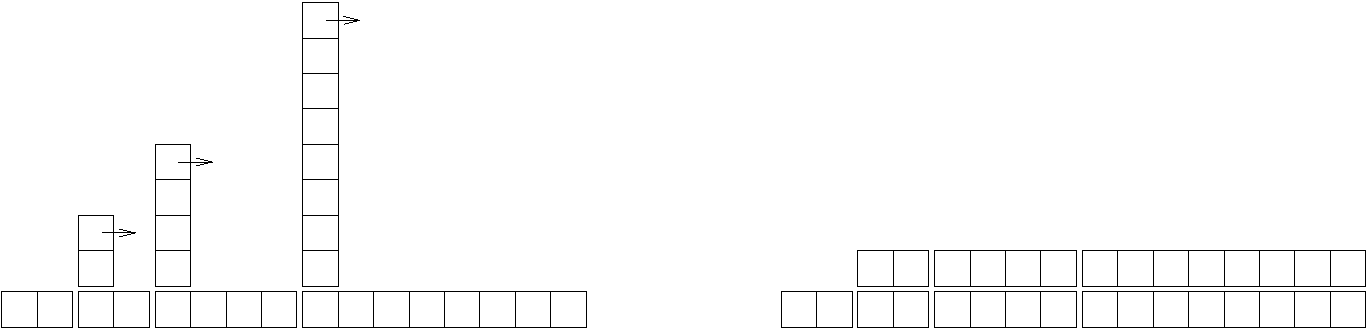
\includegraphics[scale=1.0]{figs/towers.pdf}}
\caption{The cost of a hashtable add.\label{fig.hash}}
\end{figure}

The extra work of rehashing appears as a sequence of increasingly
tall towers with increasing space between them.  Now if you knock
over the towers, amortizing the cost of resizing over all
adds, you can see graphically that the total cost after $n$
adds is $2n - 2$.

重哈希的额外工作显示为一序列增加的高塔并在它们之间增加空间。
现在,如果你打翻这些塔,将resize的代价均摊到所有的add上,
你会从图上看到$n$个add的整个花费是$2n - 2$。

An important feature of this algorithm is that when we resize the
HashTable it grows geometrically; that is, we multiply the size by a
constant.  If you increase the size
arithmetically---adding a fixed number each time---the average time
per {\tt add} is linear.
\index{geometric resizing}

You can download my implementation of HashMap from
\url{http://thinkpython/code/Map.py}, but remember that there
is no reason to use it; if you want a map, just use a Python dictionary.

该算法一个重要的特征是当我们resize哈希表的时候,
它几何级增长。也就是说,我们用常数乘以大小。
如果你按算术级增加大小---每次增加固定的数目---每个{\tt add}的平均时间是线性的。

\chapter{Lumpy}
\label{lumpy}

Throughout the book, I have used diagrams to represent the state of
running programs.
\index{Lumpy}

贯穿全书地,我使用图来表示运行的程序的状态。

In Section~\ref{variables}, we used a state diagram to show the names
and values of variables.  In Section~\ref{stackdiagram} I introduced a
stack diagram, which shows one frame for each function call.  Each
frame shows the parameters and local variables for the function or
method.  Stack diagrams for recursive functions appear in
Section~\ref{recursive.stack} and Section~\ref{more.recursion}.
\index{stack diagram} \index{diagram!stack}
\index{state diagram} \index{diagram!state}

在\ref{variables}节,我们使用状态图来显示变量的名和值。
在\ref{stackdiagram}节,我介绍了栈图,其为每个函数调用显示一个框架。
每个框架为该函数或者方法显示了形参以及局部变量。
对于递归函数的栈图出现在\ref{recursive.stack}和\ref{more.recursion}节。

Section~\ref{mutable} shows what a list looks like in a state diagram,
Section~\ref{invert} shows what a dictionary looks like, and
Section~\ref{dictuple} shows two ways to represent tuples.

\ref{mutable}节显示在栈图中,列表看起来的样子,
\ref{invert}节显示字典的样子,\ref{dictuple}节显示表示元组的两个方法。

Section~\ref{attributes} introduces object diagrams, which show the
state of an object's attributes, and their attributes, and so on.
Section~\ref{rectangles} has object diagrams for Rectangles and
their embedded Points.  Section~\ref{time.object} shows the state
of a Time object.
Section~\ref{class.attribute} has a diagram that includes a class
object and an instance, each with their own attributes.
\index{object diagram}
\index{diagram!object}

\ref{attributes}节介绍了对象图,其展示了一个对象的属性的状态以及他们的属性等。
\ref{rectangles}节有对于矩形以及他们嵌入的点的对象图。
\ref{time.object} 节显示了一个Time对象的状态。
\ref{class.attribute}有一个图,其包括一个类对象以及一个实例,每个都有他们自己的属性。

Finally, Section~\ref{class.diagram} introduces class diagrams,
which show the classes that make up a program and the relationships
between them.
\index{class diagram}
\index{diagram!class}

最后,\ref{class.diagram}节介绍了类图,其展示了组成程序的类以及它们之间的关系。

These diagrams are based on the Unified Modeling Language (UML), which
is a standardized graphical language used by software engineers
to communicate about program design, especially for object-oriented
programs.
\index{Unified Modeling Language}
\index{UML}

这些图基于统一建模语言(UML),其是一个标准的图示语言,
软件工程师用其交流程序设计,特别是对于面向对象的程序。

UML is a rich language with many kinds of diagrams that represent
many kinds of relationship between objects and classes.  What I presented
in this book is a small subset of the language, but it is the subset
most commonly used in practice.

UML是内容非常丰富的语言,具有多种图来表示许多种对象和类之间的关系。
本书中我表示的只是该语言的一个小子集,
但是它是实践中最常用的子集。

The purpose of this appendix is to review the diagrams presented in
the previous chapters, and to introduce Lumpy.  Lumpy, which stands
for ``UML in Python,'' with some of the letters rearranged, is part of
Swampy, which you already installed if you worked on the case study in
Chapter~\ref{turtlechap} or Chapter~\ref{tkinter}, or if you did
Exercise~\ref{canvas},
\index{Lumpy}
\index{Swampy}

本附录的目的是回顾之前章节中给出的图并介绍Lumpy。
Lumpy,表示``UML in Python'',是对一些字母的重排列,
是Swampy的一部分,如果你完成了第\ref{turtlechap}章或第\ref{tkinter}的案例学习,
或者做了练习\ref{canvas},你已经安装好了Swampy。

Lumpy uses Python's {\tt inspect} module to examine the state of a running
program and generate object diagrams (including stack diagrams) and
class diagrams.

Lumpy使用Python的{\tt inspect}模块来检查一个正在运行的程序的状态并生成对象图
(包括栈图)以及类图。

\section{State diagram 状态图}

\begin{figure}
\centerline
{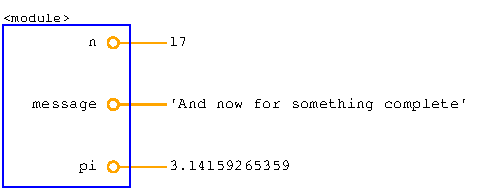
\includegraphics[scale=0.7]{figs/lumpydemo1.pdf}}
\caption{State diagram generated by Lumpy.}
\label{fig.lumpy1}
\end{figure}

Here's an example that uses Lumpy to generate a state diagram.
\index{state diagram} \index{diagram!state}

此处是一个使用Lumpy生成状态图的例子。

\begin{verbatim}
from swampy.Lumpy import Lumpy

lumpy = Lumpy()
lumpy.make_reference()

message = 'And now for something completely different'
n = 17
pi = 3.1415926535897932

lumpy.object_diagram()
\end{verbatim}

The first line imports the Lumpy class from {\tt swampy.Lumpy}.
If you don't have Swampy installed as a package, make sure
the Swampy files are in Python's search path and use this
{\tt import} statement instead:

第一行从{\tt swampy.Lumpy}导入Lumpy类。
如果你没有作为包安装Swamp,确定Swampy文件位于Python的搜索目录
并使用此{\tt import}语句代替:

\begin{verbatim}
from Lumpy import Lumpy
\end{verbatim}

The next lines create a {\tt Lumpy} object and make a ``reference''
point, which means that Lumpy records the objects that have been
defined so far.

接下来的几行生成一个{\tt Lumpy}对象并生成一个``参考''点,
其意味着Lumpy记录目前已经被定义的对象。

Next we define new variables and invoke \verb"object_diagram",
which draws the objects that have been defined since the reference
point, in this case {\tt message}, {\tt n} and {\tt pi}.

接着我们定义新的变量并调用\verb"object_diagram",
来画这些自参考点之后定义的对象。

Figure~\ref{fig.lumpy1} shows the result.  The graphical style is
different from what I showed earlier; for example, each
reference is represented by a circle next to the variable name and a
line to the value.  And long strings are truncated.  But the
information conveyed by the diagram is the same.

图\ref{fig.lumpy1}展示了结果。这个图的样式与我之前展示的不同。
例如,每个引用用一个变量名以及一个连接到值的圆表示。
长字符串被截去了。但是此图传递的信息是相同的。

The variable names are in a frame labeled \verb"<module>", which
indicates that these are module-level variables, also known as
global.
\index{global variable}
\index{variable!global}
\index{module-level variable}
\index{variable!module-level}

变量名位于一个标为 \verb"<module>"的线框里,
其指明这些是模块级的变量,也被认为是全局变量。

You can download this example from
\url{http://thinkpython.com/code/lumpy_demo1.py}.  Try adding some
additional assignments and see what the diagram looks like.

你可以从\url{http://thinkpython.com/code/lumpy_demo1.py}下载这个例子。
试着增加一些额外的赋值并看此图看起来像什么样子。


\section{Stack diagram 栈图}

\begin{figure}
\centerline
{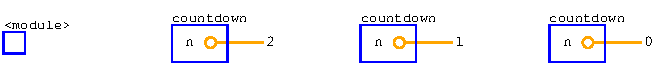
\includegraphics[scale=0.7]{figs/lumpydemo2.pdf}}
\caption{Stack diagram.}
\label{fig.lumpy2}
\end{figure}

Here's an example that uses Lumpy to generate a stack diagram.
You can download it from \url{http://thinkpython.com/code/lumpy_demo2.py}.
\index{stack diagram} 
\index{diagram!stack}

这是一个使用Lumpy生成栈图的例子。
你可以从\url{http://thinkpython.com/code/lumpy_demo2.py}下载它。

\begin{verbatim}
from swampy.Lumpy import Lumpy

def countdown(n):
    if n <= 0:
        print 'Blastoff!'
        lumpy.object_diagram()
    else:
        print n
        countdown(n-1)

lumpy = Lumpy()
lumpy.make_reference()
countdown(3)
\end{verbatim}

Figure~\ref{fig.lumpy2} shows the result.  Each frame is represented
with a box that has the function's name outside and variables inside.
Since this function is recursive, there is one frame for each
level of recursion.
\index{recursion}
\index{function frame}
\index{frame}

图\ref{fig.lumpy2}显示了结果。每个线框用一个盒子表示,它外面有函数名,
里面有变量。既然此函数是递归的,每层递归有一个线框。

Remember that a stack diagram shows the state of the program at
a particular point in its execution.  To get the diagram you want,
sometimes you have to think about where to invoke \verb"object_diagram".

记住一个栈图显示了程序在它执行中一个特定点的状态。
为了获得你希望的图,有时你必须考虑在哪儿调用\verb"object_diagram"。

In this case I invoke \verb"object_diagram" after executing the base
case of the recursion; that way the stack diagram shows each level of
the recursion.  You can call \verb"object_diagram" more than once to
get a series of snapshots of the program's execution.
\index{base case}

在这个例子中,我在执行递归的基本条件后调用\verb"object_diagram",
这使得栈图显示递归的每一层。你可以不止一次调用\verb"object_diagram"
来获得一系列程序执行的快照。


\section{Object diagrams 对象图}

\begin{figure}
\centerline
{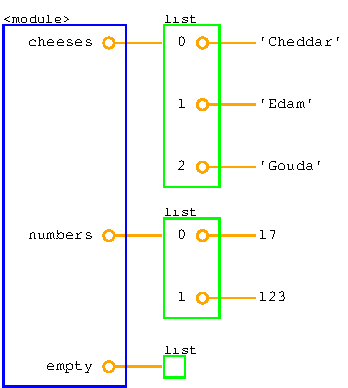
\includegraphics[scale=0.7]{figs/lumpydemo3.pdf}}
\caption{Object diagram.}
\label{fig.lumpy3}
\end{figure}

This example generates an object diagram showing the lists from
Section~\ref{sequence}.  You can download it from
\url{http://thinkpython.com/code/lumpy_demo3.py}.
\index{object diagram} 
\index{diagram!object}

此例生成一个显示来自~\ref{sequence}节列表的对象图。
你可以从\url{http://thinkpython.com/code/lumpy_demo3.py}下载它。

\begin{verbatim}
from swampy.Lumpy import Lumpy

lumpy = Lumpy()
lumpy.make_reference()

cheeses = ['Cheddar', 'Edam', 'Gouda']
numbers = [17, 123]
empty = []

lumpy.object_diagram()
\end{verbatim}

Figure~\ref{fig.lumpy3} shows the result.  Lists are represented by
a box that shows the indices mapping to the elements.  This representation
is slightly misleading, since indices are not actually
part of the list, but I think they make the diagram easier to
read.  The empty list is represented by an empty box. 
\index{list index}

图\ref{fig.lumpy3}显示结果。
列表被表示成一个盒子,展示了映射到元素的索引。
这一表示有点儿误导,因为索引不是列表的实际部分,
但是我想它们使得图更容易被读。
空列表被表示为一个空盒子。

\begin{figure}
\centerline
{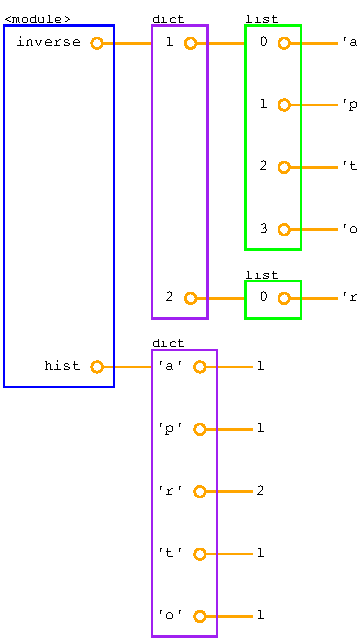
\includegraphics[scale=0.7]{figs/lumpydemo4.pdf}}
\caption{Object diagram.}
\label{fig.lumpy4}
\end{figure}

And here's an example 
showing the dictionaries from Section~\ref{invert}.  You can download
it from \url{http://thinkpython.com/code/lumpy_demo4.py}.
\index{dictionary}

这是一个显示来自\ref{invert}节的字典的例子。
你可以从\url{http://thinkpython.com/code/lumpy_demo4.py}下载它。

\begin{verbatim}
from swampy.Lumpy import Lumpy

lumpy = Lumpy()
lumpy.make_reference()

hist = histogram('parrot')
inverse = invert_dict(hist)

lumpy.object_diagram()
\end{verbatim}

Figure~\ref{fig.lumpy4} shows the result.  {\tt hist} is a dictionary
that maps from characters (single-letter strings) to integers;
{\tt inverse} maps from integers to lists of strings.

图\ref{fig.lumpy4}显示结果。
{\tt hist}是一个字典,从字符(单字母字符串)映射到整数。
{\tt inverse}从整数映射到字符串列表。

\begin{figure}
\centerline
{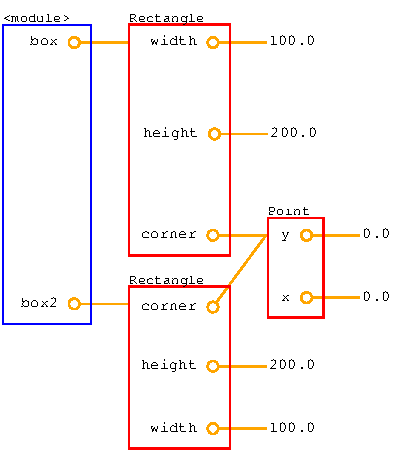
\includegraphics[scale=0.7]{figs/lumpydemo5.pdf}}
\caption{Object diagram.}
\label{fig.lumpy5}
\end{figure}

This example generates an object diagram for Point and Rectangle
objects, as in Section~\ref{copying}.  You can download it from
\url{http://thinkpython.com/code/lumpy_demo5.py}.
\index{Point class}
\index{class!Point}
\index{Rectangle class}
\index{class!Rectangle}

此例生成一个Point和Rectangle对象的对象图,如\ref{copying}节所示。
你可以从\url{http://thinkpython.com/code/lumpy_demo5.py}下载它。

\begin{verbatim}
import copy
from swampy.Lumpy import Lumpy

lumpy = Lumpy()
lumpy.make_reference()

box = Rectangle()
box.width = 100.0
box.height = 200.0
box.corner = Point()
box.corner.x = 0.0
box.corner.y = 0.0

box2 = copy.copy(box)

lumpy.object_diagram()
\end{verbatim}

Figure~\ref{fig.lumpy5} shows the result.  {\tt copy.copy} make a
shallow copy, so {\tt box} and {\tt box2} have their own {\tt width}
and {\tt height}, but they share the same embedded Point object.  This
kind of sharing is usually fine with immutable objects, but with
mutable types, it is highly error-prone.
\index{copy}
\index{shallow copy}

图\ref{fig.lumpy5}显示结果。
{\tt copy.copy}进行浅拷贝,所以{\tt box}和{\tt box2}有它们自己的{\tt width}和{\tt height},
但是它们共享相同的嵌入Point对象。
这种共享通常对于不可变对象是好的,但是对于可变类型,它非常容易出错。

\section{Function and class objects 函数和类对象}

\begin{figure}
\centerline
{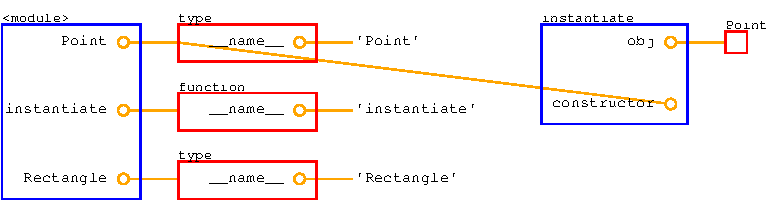
\includegraphics[scale=0.7]{figs/lumpydemo6.pdf}}
\caption{Object diagram.}
\label{fig.lumpy6}
\end{figure}

When I use Lumpy to make object diagrams, I usually define the functions
and classes before I make the reference point.  That way, function
and class objects don't appear in the diagram.
\index{function object}
\index{object!function}
\index{class object}
\index{object!class}

当我用Lumpy生成对象图时,我通常在生成参考点之前定义函数和类。
这样,函数和类对象不出现在图中。

But if you are passing functions and classes as parameters, you might
want them to appear.  This example shows what that looks like;
you can download it from
\url{http://thinkpython.com/code/lumpy_demo6.py}.

但是如果你正作为形参传递函数和类,你可能希望它们出现。
此例展示那看起来是什么样:

\begin{verbatim}
import copy
from swampy.Lumpy import Lumpy

lumpy = Lumpy()
lumpy.make_reference()

class Point(object):
    """Represents a point in 2-D space."""

class Rectangle(object):
    """Represents a rectangle."""

def instantiate(constructor):
    """Instantiates a new object."""
    obj = constructor()
    lumpy.object_diagram()
    return obj

point = instantiate(Point)
\end{verbatim}

Figure~\ref{fig.lumpy6} shows the result.  Since we invoke
\verb"object_diagram" inside a function, we get a stack diagram
with a frame for the module-level variables and for the invocation
of {\tt instantiate}.

图\ref{fig.lumpy6}显示这一结果。
既然我们在一个函数中调用\verb"object_diagram",
我们为模块级的变量和{\tt instantiate}的调用获得一个具有框架的栈图。

At the module level, {\tt Point} and {\tt Rectangle} refer to
class objects (which have type {\tt type}); {\tt instantiate}
refers to a function object.
\index{instantiate}
\index{constructor}

在模块级,{\tt Point}和{\tt Rectangle}指类对象(其类型是{\tt type})。
{\tt instantiate}指一个函数对象。

This diagram might clarify two points of common confusion: (1) the
difference between the class object, {\tt Point}, and the instance of
Point, {\tt obj}, and (2) the difference between the function object
created when {\tt instantiate} is defined, and the frame created with
it is called.

此图可能会澄清通常易混淆的两点:
(1)类对象{\tt Point}和Point的实例{\tt obj}之间的不同;
(2)当{\tt instantiate}被定义是生成的函数对象和其被调用时生成的框架之间的不同。


\section{Class Diagrams 类图}

\begin{figure}
\centerline
{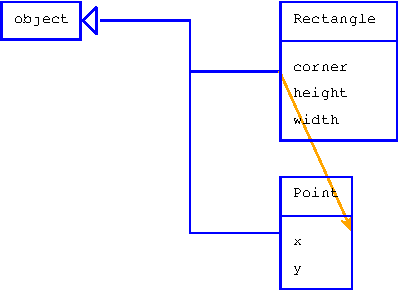
\includegraphics[scale=0.7]{figs/lumpydemo7.pdf}}
\caption{Class diagram.}
\label{fig.lumpy7}
\end{figure}

\begin{figure}
\centerline
{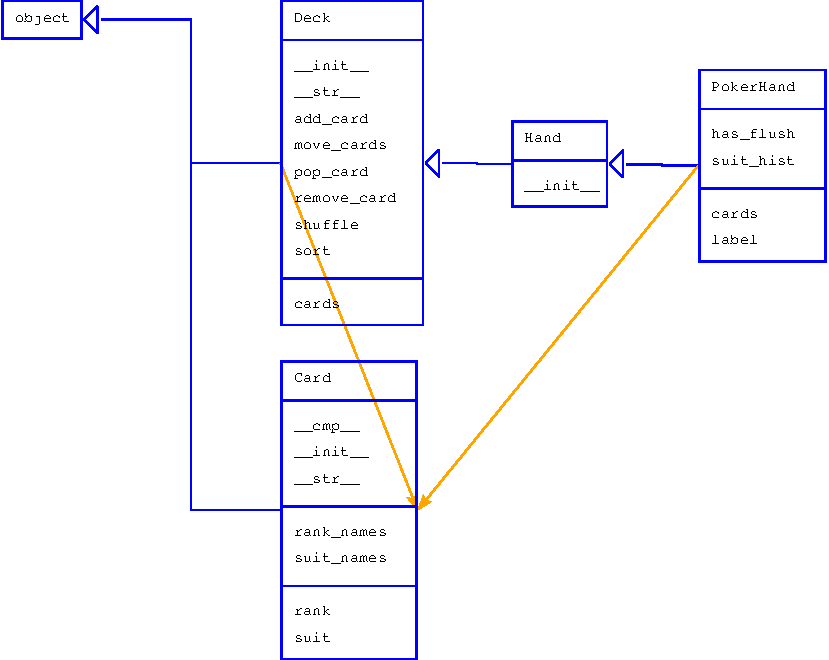
\includegraphics[scale=0.7]{figs/lumpydemo8.pdf}}
\caption{Class diagram.}
\label{fig.lumpy8}
\end{figure}

Although I distinguish between state diagrams, stack diagrams and
object diagrams, they are mostly the same thing: they show the
state of a running program at a point in time.
\index{class diagram}
\index{diagram!class}

虽然我区分了状态度、栈图以及类图,但是它们基本是同一个东西:
它们显示了一个正在运行的程序在某一时间点的状态。

Class diagrams are different.  They show the classes that make up a
program and the relationships between them.  They are timeless in the
sense that they describe the program as a whole, not any particular
point in time.  For example, if an instance of Class A generally
contains a reference to an instance of Class B, we say there is a
``HAS-A relationship'' between those classes.
\index{HAS-A relationship}
\index{class diagram}
\index{diagram!class}
\index{UML}

类图不一样。它们显示了组成程序的类以及它们之间的关系。
它们作为一个整体描述程序,在这个意义上,它们是永恒的,
不是任何特殊的时间点。例如,如果一个类A的实例通常包含类B的实例的一个引用,
我们说在这些类之间有一个``HAS-A关系''。

Here's an example that shows a HAS-A relationship.  You can download
it from \url{http://thinkpython.com/code/lumpy_demo7.py}.

这是一个展示HAS-A关系的示例。
你可以从\url{http://thinkpython.com/code/lumpy_demo7.py}下载它。

\begin{verbatim}
from swampy.Lumpy import Lumpy

lumpy = Lumpy()
lumpy.make_reference()

box = Rectangle()
box.width = 100.0
box.height = 200.0
box.corner = Point()
box.corner.x = 0.0
box.corner.y = 0.0

lumpy.class_diagram()
\end{verbatim}

Figure~\ref{fig.lumpy7} shows the result.  
Each class is represented with a box that contains the name of the
class, any methods the class provides, any class variables, and
any instance variables.  In this example, {\tt Rectangle} and {\tt Point}
have instance variables, but no methods or class variables.

图\ref{fig.lumpy7}显示了结果。每个类被表示成一个盒子,
包含类名、类提供的任何方法,类变量以及任何实例变量。
在此例中,{\tt Rectangle}和{\tt Point}有实例变量,
但是没有方法或类变量。

The arrow from {\tt Rectangle} to {\tt Point} shows that Rectangles
contain an embedded Point.  In addition, {\tt Rectangle} and {\tt
  Point} both inherit from {\tt object}, which is represented in
the diagram with a triangle-headed arrow.
\index{IS-A relationship}

从{\tt Rectangle}到{\tt Point}的箭头显示Rectangles包含一个嵌入的Point。
另外,{\tt Rectangle}和{\tt Point}都是继承自{\tt object},
这在图中用一个三角头的箭头表示。

Here's a more complex example using my solution to Exercise~\ref{poker}.
You can download
the code from \url{http://thinkpython.com/code/lumpy_demo8.py};
you will also need \url{http://thinkpython.com/code/PokerHand.py}.

这是一个更复杂的例子,使用了我的习题\ref{poker}的答案。
你从\url{http://thinkpython.com/code/lumpy_demo8.py}可以下载代码;
你也需要\url{http://thinkpython.com/code/PokerHand.py}。

\begin{verbatim}
from swampy.Lumpy import Lumpy

from PokerHand import *

lumpy = Lumpy()
lumpy.make_reference()

deck = Deck()
hand = PokerHand()
deck.move_cards(hand, 7)

lumpy.class_diagram()
\end{verbatim}

Figure~\ref{fig.lumpy8} shows the result.  
{\tt PokerHand} inherits from {\tt Hand}, which inherits from {\tt Deck}.
Both {\tt Deck} and {\tt PokerHand} have Cards.
\index{Card class}
\index{Deck class}
\index{Hand class}

图\ref{fig.lumpy8}显示了结果。
{\tt PokerHand}继承自{\tt Hand},它继承自{\tt Deck}。
{\tt Deck}和{\tt PokerHand}都有Cards。

This diagram does not show that {\tt Hand} also has cards, because
in the program there are no instances of Hand.  This example
demonstrates a limitation of Lumpy; it only knows about the
attributes and HAS-A relationships of objects that are instantiated.

此图没有显示{\tt Hand}也有cards,因为在这个程序中,没有Hand的实例。
此例展示了Lumpy的一个局限性,它只知道被实例化的对象的属性和HAS-A关系。

\printindex

\clearemptydoublepage
%\blankpage
%\blankpage
%\blankpage

\ifxetex
\else
\end{CJK}
\fi
\end{document}
